\documentclass[12pt,a4paper]{extarticle}

% ==========================================
% PACOTES UTILIZADOS
% ==========================================
\usepackage[utf8]{inputenc}
\usepackage[T1]{fontenc}
\usepackage[english,portuguese]{babel}
\usepackage{setspace}
\usepackage{geometry}
\usepackage{graphicx}
\usepackage{xurl}
\usepackage{helvet}
\usepackage{amsmath}
\usepackage{amssymb}
\usepackage{array}
\usepackage{tabularx}
\usepackage{tikz}
\usepackage{xcolor}
\usepackage{booktabs}
\usepackage{ragged2e}
\usepackage{longtable}
\usepackage{array}
\usepackage{tocloft}
\usepackage{float}
\usepackage{caption}
\usepackage{xltabular}   % tabelas longas que quebram de pagina
\usepackage{pdflscape}   % paginas em paisagem (diagramas grandes)
\usepackage{placeins}    % \FloatBarrier
\usepackage{listings}    % codigo nos apendices (DDL, config.yml)
\emergencystretch=3em    % reduz linhas estouradas (Overfull) sem alterar o texto
\renewcommand{\familydefault}{\sfdefault}
\geometry{a4paper, left=3cm, top=3cm, right=2cm, bottom=2cm}
\usepackage{indentfirst}
\usepackage{newunicodechar}
\newunicodechar{≠}{\ensuremath{\neq}}
\usepackage{hyperref}
\hypersetup{
    colorlinks=true,
    linkcolor=black,
    urlcolor=black,
    citecolor=black
}

% CORRIGIDO: o texto do trabalho chama os diagramas de "Figura N" (13 vezes); manter "Gráfico" nas legendas
% gerava "Gráfico 10" na legenda e "Figura 10" no texto. Para voltar a "Gráfico", reverta estas 2 linhas
% (e troque "Figura~\ref" por "Gráfico~\ref" no texto).
\renewcommand{\listfigurename}{\centerline{LISTA DE FIGURAS}}
\renewcommand{\listtablename}{\centerline{LISTA DE TABELAS}}

\newlistof{myequations}{equ}{Lista de Equações}

% Mesmo alinhamento da Lista de Figuras/Tabelas
\setlength{\cftmyequationsindent}{\cftfigindent}
\setlength{\cftmyequationsnumwidth}{\cftfignumwidth}

% \dado{...} marca campos a preencher (em vermelho). Na versao FINAL troque \rascunhotrue por \rascunhofalse:
% se sobrar qualquer campo marcado com dado o PDF NAO compila (impede entregar "[N]" em vermelho por engano).
\newif\ifrascunho
\rascunhofalse
\newcommand{\dado}[1]{\ifrascunho\textcolor{red}{[#1]}\else\PackageError{tcc}{Dado pendente nao resolvido: \detokenize{#1}}{Resolva todos os campos marcados como dado antes da versao final.}\fi}
\lstset{basicstyle=\ttfamily\footnotesize,breaklines=true,columns=fullflexible,frame=single,extendedchars=true,
  literate={á}{{\'a}}1 {é}{{\'e}}1 {í}{{\'i}}1 {ó}{{\'o}}1 {ú}{{\'u}}1 {ã}{{\~a}}1 {õ}{{\~o}}1 {ç}{{\c c}}1
           {â}{{\^a}}1 {ê}{{\^e}}1 {ô}{{\^o}}1 {à}{{\`a}}1 {Á}{{\'A}}1 {É}{{\'E}}1 {Í}{{\'I}}1 {Ó}{{\'O}}1
           {Ú}{{\'U}}1 {Ã}{{\~A}}1 {Ç}{{\c C}}1 {—}{{---}}1 {–}{{--}}1 {→}{{->}}1}

% Comando para adicionar equações à lista
\newcommand{\myequation}[1]{
    \addcontentsline{equ}{myequations}
    {\protect\numberline{\theequation}#1}
}
% Configuração de parágrafo ABNT
\setlength{\parindent}{1.5cm}

% Formatação das tabelas do dicionário de dados
\newcolumntype{L}[1]{>{\raggedright\arraybackslash}p{#1}}
\newcolumntype{Y}{>{\raggedright\arraybackslash}X}
\renewcommand{\arraystretch}{1.2}
\setlength{\tabcolsep}{4pt}

\begin{document}

% ==========================================
% CAPA
% ==========================================
\begin{titlepage}
    \begin{center}
        \textbf{Centro Universitário Dinâmica das Cataratas}\\
        \textbf{Curso de Bacharelado em Sistemas de Informação}\\
        \vspace{3cm}

        \textbf{ADNAN OMAR JIBARA}\\

        \vspace{3cm}
        \textbf{Trabalho de Conclusão de Curso}\\
        \vspace{0.5cm}
        % TÍTULO ANTIGO (revisão pré-banca: título extenso e promete produto completo;
        % sugestão do orientador e da avaliação: reduzir e delimitar o escopo como protótipo,
        % sem citar tecnologias/ferramentas específicas no título)
        %\textbf{ANÁLISE, MODELAGEM E DESENVOLVIMENTO DE UM CHATBOT BASEADO EM INTELIGÊNCIA ARTIFICIAL PARA AUTOMAÇÃO DE PROCESSOS ADMINISTRATIVOS E OTIMIZAÇÃO DO AGENDAMENTO DE CONSULTAS EM CLÍNICAS MÉDICAS}\\
        % TÍTULO NOVO
        \textbf{DESENVOLVIMENTO DE UM PROTÓTIPO DE CHATBOT BASEADO EM INTELIGÊNCIA ARTIFICIAL PARA AUTOMAÇÃO DO AGENDAMENTO DE CONSULTAS EM CLÍNICAS DE PEQUENO E MÉDIO PORTE}\\

        \vspace{3cm}
        \begin{flushright}
        \begin{minipage}{8cm}
            Trabalho de Conclusão de Curso apresentado ao Curso de Bacharelado em Sistemas de Informação do Centro Universitário Dinâmica das Cataratas (UDC) como requisito parcial para obtenção do título de bacharel em Sistemas de Informação.\\

            Orientador: Prof. Me. Luciano Santos Cardoso
            \vspace{3cm}
        \end{minipage}
        \end{flushright}

        \vfill
        \textbf{Foz do Iguaçu - PR}\\
        \textbf{2026}
    \end{center}
\end{titlepage}


% ==========================================
% RESUMO
% ==========================================
\newpage
\thispagestyle{empty}
\begin{center}
    \textbf{RESUMO}
\end{center}
\vspace{0.5cm}

\noindent O agendamento de consultas em clínicas de pequeno e médio porte costuma depender de atendimento telefônico e presencial, o que sobrecarrega a recepção e prolonga a espera do paciente. Este trabalho teve como objetivo desenvolver e avaliar, em ambiente simulado, um protótipo de chatbot baseado em Inteligência Artificial capaz de automatizar o agendamento, o cancelamento e o reagendamento de consultas, com tratamento de dados de saúde aderente à Lei Geral de Proteção de Dados (LGPD). A pesquisa, de natureza aplicada e abordagem quali-quantitativa, seguiu a \textit{Design Science Research}. O protótipo foi implementado com Rasa Open Source, modelo BERTimbau para o português brasileiro, banco de dados SQLite e Telegram como canal, com execução local do núcleo do sistema, diálogo conduzido por regras e formulários e consentimento registrado por finalidade. O módulo de compreensão de linguagem natural foi avaliado com um corpus sintético de 703 frases em 21 intenções. Na validação cruzada com cinco partições repetida três vezes, a acurácia média foi de 86,3\% e o F1-score médio (macro) de 0,85; no conjunto de teste, 87,9\% e 0,86, respectivamente. Na comparação com e sem o BERTimbau nas mesmas partições, o modelo elevou a acurácia média em 2,9 pontos percentuais e o F1-score em 0,032; com o teste $t$ corrigido para validação cruzada, a diferença foi significativa para a acurácia (p = 0,035), mas não para o F1-score (p = 0,076). O tempo médio de resposta do servidor foi de 0,31 s, e os fluxos de agendamento, consulta e cancelamento foram concluídos em todos os 26 ciclos automatizados. Nos testes funcionais, as 74 execuções de 26 cenários foram concluídas com sucesso, após três ciclos de refinamento, motivados por falhas encontradas nos próprios testes e na depuração e revisão do protótipo. A pontuação média na escala de usabilidade SUS (\textit{System Usability Scale}) foi de 87,5 ($n = 5$). Os resultados indicam a viabilidade técnica da abordagem em ambiente simulado, mas não permitem afirmar redução de tempo de espera ou de custo em clínicas reais, o que fica como trabalho futuro. Entre as limitações estão o uso de dados sintéticos, o canal de mensageria externo e a integração simulada com o padrão HL7 FHIR.

\vspace{0.5cm}
\noindent \textbf{Palavras-chave:} Chatbot. Agendamento de consultas. Processamento de Linguagem Natural. Rasa. LGPD.

% ==========================================
% ABSTRACT
% ==========================================
\newpage
\begin{otherlanguage}{english}
\thispagestyle{empty}
\begin{center}
    \textbf{ABSTRACT}
\end{center}
\vspace{0.5cm}

\noindent Appointment scheduling in small and medium-sized clinics usually relies on phone calls and in-person service, which overloads reception staff and lengthens patients' waiting time. This work aimed to develop and evaluate, in a simulated environment, an Artificial Intelligence-based chatbot prototype able to automate the scheduling, cancellation and rescheduling of medical appointments, handling health data in line with the Brazilian General Data Protection Law (LGPD). The research is applied, with a mixed qualitative-quantitative approach, and followed Design Science Research. The prototype was implemented with Rasa Open Source, the BERTimbau model for Brazilian Portuguese, an SQLite database and Telegram as the channel, with local execution of the system core, rule- and form-based dialogue management and purpose-specific consent records. The natural language understanding module was evaluated on a synthetic corpus of 703 utterances across 21 intents. Under five-fold cross-validation repeated three times, mean accuracy was 86.3\% and the macro-averaged F1-score was 0.85; on the test set, 87.9\% and 0.86, respectively. Compared on the same partitions, BERTimbau raised mean accuracy by 2.9 percentage points and the F1-score by 0.032; with the corrected resampled $t$-test, the difference was significant for accuracy (p = 0.035) but not for the F1-score (p = 0.076). The mean server response time was 0.31 s, and the scheduling, lookup and cancellation flows were completed in all 26 automated cycles. In the functional tests, all 74 runs of 26 scenarios succeeded, after three refinement cycles, driven by faults found by the tests themselves and by debugging and reviewing the prototype. The mean SUS score was 87.5 ($n = 5$). The results indicate the technical feasibility of the approach in a simulated environment, but do not allow claiming reductions in waiting time or cost in real clinics, which is left for future work. Limitations include synthetic data, an external messaging channel and a simulated HL7 FHIR integration.

\vspace{0.5cm}
\noindent \textbf{Keywords:} Chatbot. Appointment scheduling. Natural Language Processing. Rasa. LGPD.
\end{otherlanguage}

% ==========================================
% LISTA DE ABREVIATURAS
% ==========================================
\newpage
\setcounter{page}{1}
\begin{center}
    \textbf{LISTA DE ABREVIATURAS E SIGLAS}
\end{center}
\vspace{1cm}

\begin{xltabular}{\textwidth}{@{}p{1.6cm}Y@{}}
\textbf{3FN} & Terceira Forma Normal \\
\textbf{AIML} & Artificial Intelligence Markup Language (Linguagem de Marcação de Inteligência Artificial) \\
\textbf{API} & Application Programming Interface (Interface de Programação de Aplicações) \\
\textbf{BERT} & Bidirectional Encoder Representations from Transformers (Representações de Codificador de Transformadores) \\
\textbf{BFSI} & Banking, Financial Services and Insurance (Serviços bancários, financeiros e de seguros) \\
\textbf{BPM} & Business Process Management (Gestão de Processos de Negócio) \\
\textbf{CAGR} & Compound Annual Growth Rate (Taxa de Crescimento Anual Composta) \\
\textbf{DDL} & Data Definition Language (Linguagem de Definição de Dados) \\
\textbf{DIET} & Dual Intent and Entity Transformer \\
\textbf{DL} & Deep Learning (Aprendizado Profundo) \\
\textbf{DSR} & Design Science Research (Design Science Research) \\
\textbf{EHR} & Electronic Health Records (Registros Eletrônicos de Saúde) \\
\textbf{FAQs} & Frequently Asked Questions (Perguntas frequentes) \\
\textbf{FHIR} & Fast Healthcare Interoperability Resources (Recursos de interoperabilidade rápida em saúde) \\
\textbf{FK} & Foreign Key (Chave Estrangeira) \\
\textbf{GPT} & Generative Pre-trained Transformer (Transformer generativo pré-treinado) \\
\textbf{HL7} & Health Level Seven \\
\textbf{HTTPS} & Hypertext Transfer Protocol Secure \\
\textbf{IA} & Inteligência Artificial \\
\textbf{JSON} & JavaScript Object Notation \\
\textbf{LGPD} & Lei Geral de Proteção de Dados \\
\textbf{LLM} & Large Language Model (Modelo de Linguagem de Larga Escala) \\
\textbf{LSTM} & Long Short-Term Memory (Memória de Longo e Curto Prazo) \\
\textbf{mBERT} & Multilingual BERT (BERT multilíngue) \\
\textbf{MER} & Modelo de Entidade-Relacionamento \\
\textbf{MIT} & Massachusetts Institute of Technology (Instituto de Tecnologia de Massachusetts) \\
\textbf{ML} & Machine Learning (Aprendizado de Máquina) \\
\textbf{NER} & Named Entity Recognition (Reconhecimento de Entidades Nomeadas) \\
\textbf{NLU} & Natural Language Understanding (Compreensão de Linguagem Natural) \\
\textbf{OE} & Objetivo Específico \\
\textbf{PK} & Primary Key (Chave Primária) \\
\textbf{PLN} & Processamento de Linguagem Natural \\
\textbf{REST} & Representational State Transfer (Transferência de Estado Representacional) \\
\textbf{RF} & Requisito Funcional \\
\textbf{RNF} & Requisito Não Funcional \\
\textbf{RNN} & Redes Neurais Recorrentes \\
\textbf{RPA} & Robotic Process Automation (Automação Robótica de Processos) \\
\textbf{RTE} & Recognizing Textual Entailment (Reconhecimento de Implicação Textual) \\
\textbf{SaaS} & Software as a Service (Software como serviço) \\
\textbf{SDK} & Software Development Kit \\
\textbf{SSL} & Secure Sockets Layer (Camada de Soquetes Seguros) \\
\textbf{STS} & Semantic Textual Similarity (Similaridade Textual de Sentenças) \\
\textbf{SUS} & \textit{System Usability Scale} (escala de usabilidade de sistemas; não confundir com o Sistema Único de Saúde) \\
\textbf{TI} & Tecnologia da Informação \\
\textbf{TLS} & Transport Layer Security (Segurança da Camada de Transporte) \\
\textbf{UML} & Unified Modeling Language (Linguagem de Modelagem Unificada) \\
\textbf{VC} & Validação Cruzada \\
\textbf{XML} & eXtensible Markup Language (Linguagem de Marcação Extensível) \\
\end{xltabular}
\addtocounter{table}{-1}% a lista de siglas nao e uma tabela numerada

% ==========================================
% LISTA DE GRÁFICOS
% ==========================================
\newpage
\listoffigures

% ==========================================
% LISTA DE TABELAS
% ==========================================
\newpage
\listoftables


% ==========================================
% LISTA DE Equações
% ==========================================
\newpage

\noindent{\fontsize{17}{20}\selectfont\bfseries Lista de Equações}

\vspace{0.5cm}

\makeatletter
\@starttoc{equ}
\makeatother


% ==========================================
% SUMÁRIO
% ==========================================
\newpage
\renewcommand{\contentsname}{\centerline{SUMÁRIO}}
\tableofcontents

\newpage
\onehalfspacing

% ==========================================
% INTRODUÇÃO
% ==========================================
\section{Introdução}
\label{cap:intro}
Com o passar dos anos, agendar uma consulta em uma clínica mudou drasticamente. Antigamente, o agendamento era feito pessoalmente, podendo demandar um grande tempo de espera. O processo era feito à mão, sujeito a perda de documentos e confusão devido à grande quantidade de pessoas registradas, uma vez que a ausência de estruturação e automação em processos administrativos tende a aumentar a exposição a falhas e retrabalho (WESKE, 2019). O sistema de organização era realizado pelos funcionários, sendo vulnerável a erros humanos.

O avanço da tecnologia tem impactado significativamente os meios de atendimento em diversos setores da sociedade. Na década de 1960 Joseph Weizenbaum introduziu a ``ELIZA'', o primeiro chatbot: ``Um programa de computador projetado para simular uma conversa com usuários humanos, especialmente pela internet'' (ADAMOPOULOU; MOUSSIADES, 2020). Esses sistemas têm sido adotados em comércio eletrônico, serviços bancários e suporte ao cliente, pois são eficazes na automação de tarefas repetitivas e na otimização da experiência do usuário.

Na área da saúde, os chatbots e demais soluções de automação assistida por Inteligência Artificial vêm sendo aplicados para esclarecimento de dúvidas, gestão de agendamentos e redução de faltas (\textit{no-show}). Li et al. (2021), em estudo retrospectivo com 12.342 atendimentos ambulatoriais, demonstraram que um módulo de IA responsável por antecipar a solicitação de exames antes da consulta reduziu o tempo médio entre o registro e o preparo do paciente de 1,97 horas para 0,38 horas, resultado estatisticamente significativo. De forma complementar, AlSerkal et al. (2025), em estudo conduzido em centros de atenção primária dos Emirados Árabes Unidos, mostraram que um sistema orientado por IA e integrado ao prontuário eletrônico reduziu simultaneamente a taxa de faltas e o tempo médio de espera dos pacientes, evidenciando o potencial da IA aplicada especificamente à gestão de agendamentos. Esses resultados, porém, foram obtidos em contextos de maior porte, como um serviço ambulatorial com mais de 12 mil atendimentos analisados e uma rede de atenção primária com sistema integrado ao prontuário eletrônico, e não se estendem diretamente a clínicas de pequeno e médio porte. 

Para esse segmento, interessa investigar soluções que funcionem com recursos limitados: de baixo custo, executáveis localmente e capazes de se conectar aos processos internos da clínica, como o agendamento e o cadastro de pacientes. Essa necessidade constitui o problema de pesquisa deste trabalho.

\subsection{Problema}
Em que medida um protótipo de chatbot baseado em Processamento de Linguagem Natural, executado localmente com Rasa Open Source e BERTimbau, consegue automatizar o agendamento, o cancelamento e o reagendamento de consultas em clínicas de pequeno e médio porte (cenário de aplicação: Foz do Iguaçu e região), em ambiente simulado, com desempenho de compreensão de linguagem, taxa de aprovação nos cenários de teste e usabilidade aceitáveis e em aderência aos requisitos da LGPD? A redução do tempo de espera e do custo operacional em relação aos processos manuais, embora seja a motivação do trabalho, não é medida nesta pesquisa e é indicada como trabalho futuro (seção~\ref{sec:trabalhos-futuros}).

\subsection{Justificativa}
O agendamento de consultas médicas é a base para que o paciente seja atendido por um médico, e sua gestão ineficiente compromete diretamente a experiência do usuário e a operação da clínica. Do ponto de vista prático, a evolução da tecnologia e a expansão da Tecnologia da Informação nas áreas comerciais, hoje entendida como investimento estratégico, evidenciam a necessidade de automatizar o atendimento ao cliente, considerando que muitas clínicas lidam com grande volume de ligações, mensagens e cancelamentos de consultas, gerando sobrecarga tanto para a clínica quanto para o paciente (NEWBOULD et al., 2019).

% TRECHO ANTIGO (revisão pré-banca: repetição quase mecânica da mesma estatística de
% Li et al. e AlSerkal et al. já apresentada por extenso na Introdução)
%Estudos recentes reforçam esse cenário: Li et al. (2021) demonstraram que um módulo de IA aplicado ao fluxo ambulatorial reduziu significativamente o tempo de espera entre registro e atendimento, e AlSerkal et al. (2025) evidenciaram que sistemas de IA integrados à gestão de agendamentos reduzem simultaneamente faltas e tempo de espera em unidades de atenção primária.

% TRECHO NOVO (varia a redação e evita repetir os números já apresentados na Introdução)
Os achados de Li et al. (2021) e AlSerkal et al. (2025), já apresentados na Introdução, indicam que esse tipo de sobrecarga não é exclusivo do contexto local: trata-se de um padrão observado tanto em grandes centros ambulatoriais quanto em unidades de atenção primária de outros países, o que reforça que a automação assistida por IA endereça um problema estrutural do atendimento em saúde, e não uma particularidade isolada das clínicas de Foz do Iguaçu e região.

Do ponto de vista científico, o tema apresenta relevância crescente: Rejeb (2025), em análise bibliométrica de 331 artigos publicados entre 2018 e 2024, identificou crescimento constante das publicações sobre chatbots, com pico em 2023 e 2024, o que evidencia a consolidação do tema como objeto de estudo em múltiplas áreas do conhecimento. Ainda assim, a literatura carece de soluções específicas para clínicas de pequeno e médio porte que combinem integração a sistemas de agendamento, personalização de respostas via Processamento de Linguagem Natural e conformidade com a Lei Geral de Proteção de Dados (LGPD) lacuna que este trabalho busca endereçar.

Por fim, do ponto de vista legal e de gestão de risco, a justificativa do projeto também se sustenta na necessidade de tratamento adequado de dados sensíveis de saúde, categoria expressamente prevista pela LGPD (art. 5º, II), o que torna a conformidade legal não apenas um requisito técnico do sistema, mas um elemento central de sua viabilidade e legitimidade em um contexto clínico real.

\subsection{Objetivos}

\subsubsection{Objetivo Geral}

% OBJETIVO GERAL ANTIGO (revisão pré-banca: termos como "otimizar", "melhorar a
% eficiência" e "melhorar a experiência do usuário" sem critério mensurável associado)
%Desenvolver um sistema baseado em Inteligência Artificial, por meio da implementação de um chatbot inteligente, capaz de automatizar o processo de agendamento de consultas médicas em clínicas, visando reduzir o tempo de espera dos pacientes, otimizar os processos administrativos e melhorar a eficiência operacional e a experiência do usuário no atendimento digital.

% OBJETIVO GERAL NOVO
Desenvolver e avaliar um protótipo de chatbot baseado em Inteligência Artificial, capaz de automatizar o agendamento, o cancelamento e o reagendamento de consultas médicas em clínicas de pequeno e médio porte, em ambiente simulado, mensurando seu desempenho por meio de métricas objetivas de compreensão de linguagem natural e de usabilidade, conforme detalhado na Tabela~\ref{tab:criterios-sucesso}.

% TABELA NOVA (resolve apontamento da pré-banca: termos vagos sem critério mensurável)
% TABELA FORMATADA EM PADRÃO ABNT (sem bordas verticais)
\begin{table}[H]
\centering
\caption{Critérios de sucesso mensuráveis para os termos do objetivo geral}
\label{tab:criterios-sucesso}
\begin{tabular}{p{3.5cm}p{9.5cm}}
\hline
\textbf{Termo do objetivo} & \textbf{Critério mensurável adotado} \\
\hline
Eficiência do NLU & F1-score macro $\geq$ 0,80 (média entre as intenções), reportado na validação cruzada ($k=5$, repetida com três sementes), adotada como estimador principal por ser a mais estável, e no conjunto de teste (80/20); acurácia de intenção $\geq$ 85\% (RNF04). Os valores por intenção são apresentados individualmente, sem exigir que todas atinjam 0,80 \\
Baixo custo / execução acessível & Núcleo do sistema (NLU, diálogo, ações e banco de dados) executado 100\% localmente (Rasa Open Source), sem custos de licenciamento ou de requisição a serviços em nuvem; o canal de mensageria (Telegram) é externo, o que constitui limitação declarada (seção~\ref{sec:limitacoes}) \\
Melhoria na experiência do usuário & Pontuação SUS $\geq$ 68 (média de referência da literatura), avaliada conforme a seção~\ref{sec:metricas-metodo} \\
Redução de sobrecarga / tempo de atendimento & Taxa de aprovação nos cenários de teste simulados $\geq$ 85\%; a redução efetiva de tempo e de custo em clínicas reais não é medida neste trabalho (seção~\ref{sec:trabalhos-futuros}) \\
\hline
\end{tabular}
\vspace{0.3cm}

\footnotesize{Fonte: Elaborado pelo autor, 2026.}
\end{table}

\subsubsection{Objetivos Específicos}

% OBJETIVOS ESPECÍFICOS ANTIGOS (revisão pré-banca: termos considerados vagos —
% "analisar", "modelar" e "implementar" sem indicar o que será entregue nem quais
% tecnologias/critérios serão usados; ver apontamentos do orientador e da avaliação)
%\begin{itemize}
%    \item 1. Analisar os principais processos administrativos de uma clínica que podem ser automatizados por meio de um chatbot;
%    \item 2. Modelar a arquitetura do sistema, definindo fluxos de conversação, regras de negócio, integração com sistema de agendamento e diretrizes de conformidade com a LGPD para o tratamento de dados sensíveis de saúde;
%    \item 3. Implementar o chatbot utilizando tecnologias adequadas de desenvolvimento e processamento de linguagem natural;
%    \item 4. Realizar testes funcionais para avaliar o desempenho, usabilidade e eficiência da solução desenvolvida, utilizando o protocolo SUS (\textit{System Usability Scale}) como instrumento de avaliação de usabilidade.
%\end{itemize}

% OBJETIVOS ESPECÍFICOS NOVOS
\begin{itemize}
    \item 1. Analisar, por meio de levantamento bibliográfico e documental, os principais processos administrativos de clínicas de pequeno e médio porte que podem ser automatizados por meio de um chatbot, identificando aqueles que geram maior sobrecarga operacional e apresentam maior viabilidade de automação;
    \item 2. Projetar a arquitetura do chatbot, definindo fluxos de conversação, regras de negócio, integração com o sistema de agendamento simulado e diretrizes de conformidade com a LGPD para o tratamento de dados sensíveis de saúde;
    \item 3. Implementar o chatbot utilizando o framework Rasa Open Source, o modelo de linguagem BERTimbau para o Processamento de Linguagem Natural em português, e banco de dados local para persistência segura das informações;
    \item 4. Avaliar o desempenho, a usabilidade e a eficiência da solução desenvolvida por meio de métricas objetivas: precisão, revocação e F1-score do módulo de compreensão de linguagem natural, taxa de aprovação nos cenários de teste simulados, e pontuação obtida no protocolo SUS (\textit{System Usability Scale}).
\end{itemize}

\newpage
% ==========================================
% REFERENCIAL TEÓRICO
% ==========================================
\section{Referencial Teórico}
\label{cap:referencial}

% ------------------------------------------
\subsection{Chatbots}
% ------------------------------------------

Chatbots são programas computacionais projetados para simular interações humanas por meio de linguagem natural, em interfaces de texto ou voz. De acordo com Adamopoulou e Moussiades (2020), esses sistemas podem ser definidos como programas de computador concebidos para simular conversas com usuários humanos, especialmente pela internet, e têm sido amplamente adotados em setores como comércio eletrônico, serviços bancários e suporte ao cliente, em razão de sua capacidade de automatizar tarefas repetitivas e otimizar a experiência do usuário.

Historicamente, o primeiro chatbot reconhecido foi o ELIZA, desenvolvido por Joseph Weizenbaum no Instituto de Tecnologia de Massachusetts (MIT) em 1966. O sistema operava por reconhecimento de padrões e scripts predefinidos, sendo o mais famoso o script ``DOCTOR'', concebido para simular um psicoterapeuta rogeriano. Embora primitivo sob a ótica atual, o ELIZA estabeleceu as bases conceituais para os sistemas conversacionais modernos (WEIZENBAUM, 1966).

Nos dias atuais, chatbots vêm sendo cada vez mais comuns. Isso se dá por serem soluções de baixo custo, com disponibilidade 24/7 e alta escalabilidade, atendendo milhares de usuários sem aumento proporcional de equipe.

Os chatbots evoluíram de sistemas baseados em regras rígidas para arquiteturas híbridas e, mais recentemente, para modelos de linguagem de larga escala (LLMs) sustentados por redes neurais profundas. Essa trajetória reflete o amadurecimento simultâneo de três campos: o Processamento de Linguagem Natural (PLN), o aprendizado de máquina e a disponibilidade de grandes volumes de dados para treinamento. Rejeb (2025), em análise bibliométrica de 331 artigos científicos publicados entre 2018 e 2024, identificou crescimento constante nas publicações sobre chatbots, com pico em 2023 e 2024, o que evidencia a consolidação do tema como objeto de estudo relevante em múltiplas áreas do conhecimento.

O interesse em chatbots vem crescendo bastante no mundo, isso é refletido no mercado global. Conforme projeções da Mordor Intelligence (2026), a área deve crescer de US\$ 9,30 bilhões em 2025 para US\$ 32,45 bilhões em 2031, representando uma taxa de crescimento anual composta (CAGR) de 23,15\%, conforme ilustrado na Figura~\ref{fig:mercado}. Dados complementares da Data Bridge Market Research (2024) sustentam essa tendência, mostrando um crescimento constante em várias partes do mundo.

%\begin{figure}[h!]
    %\centering
   % \caption{Projeção do mercado global de chatbots}
  %  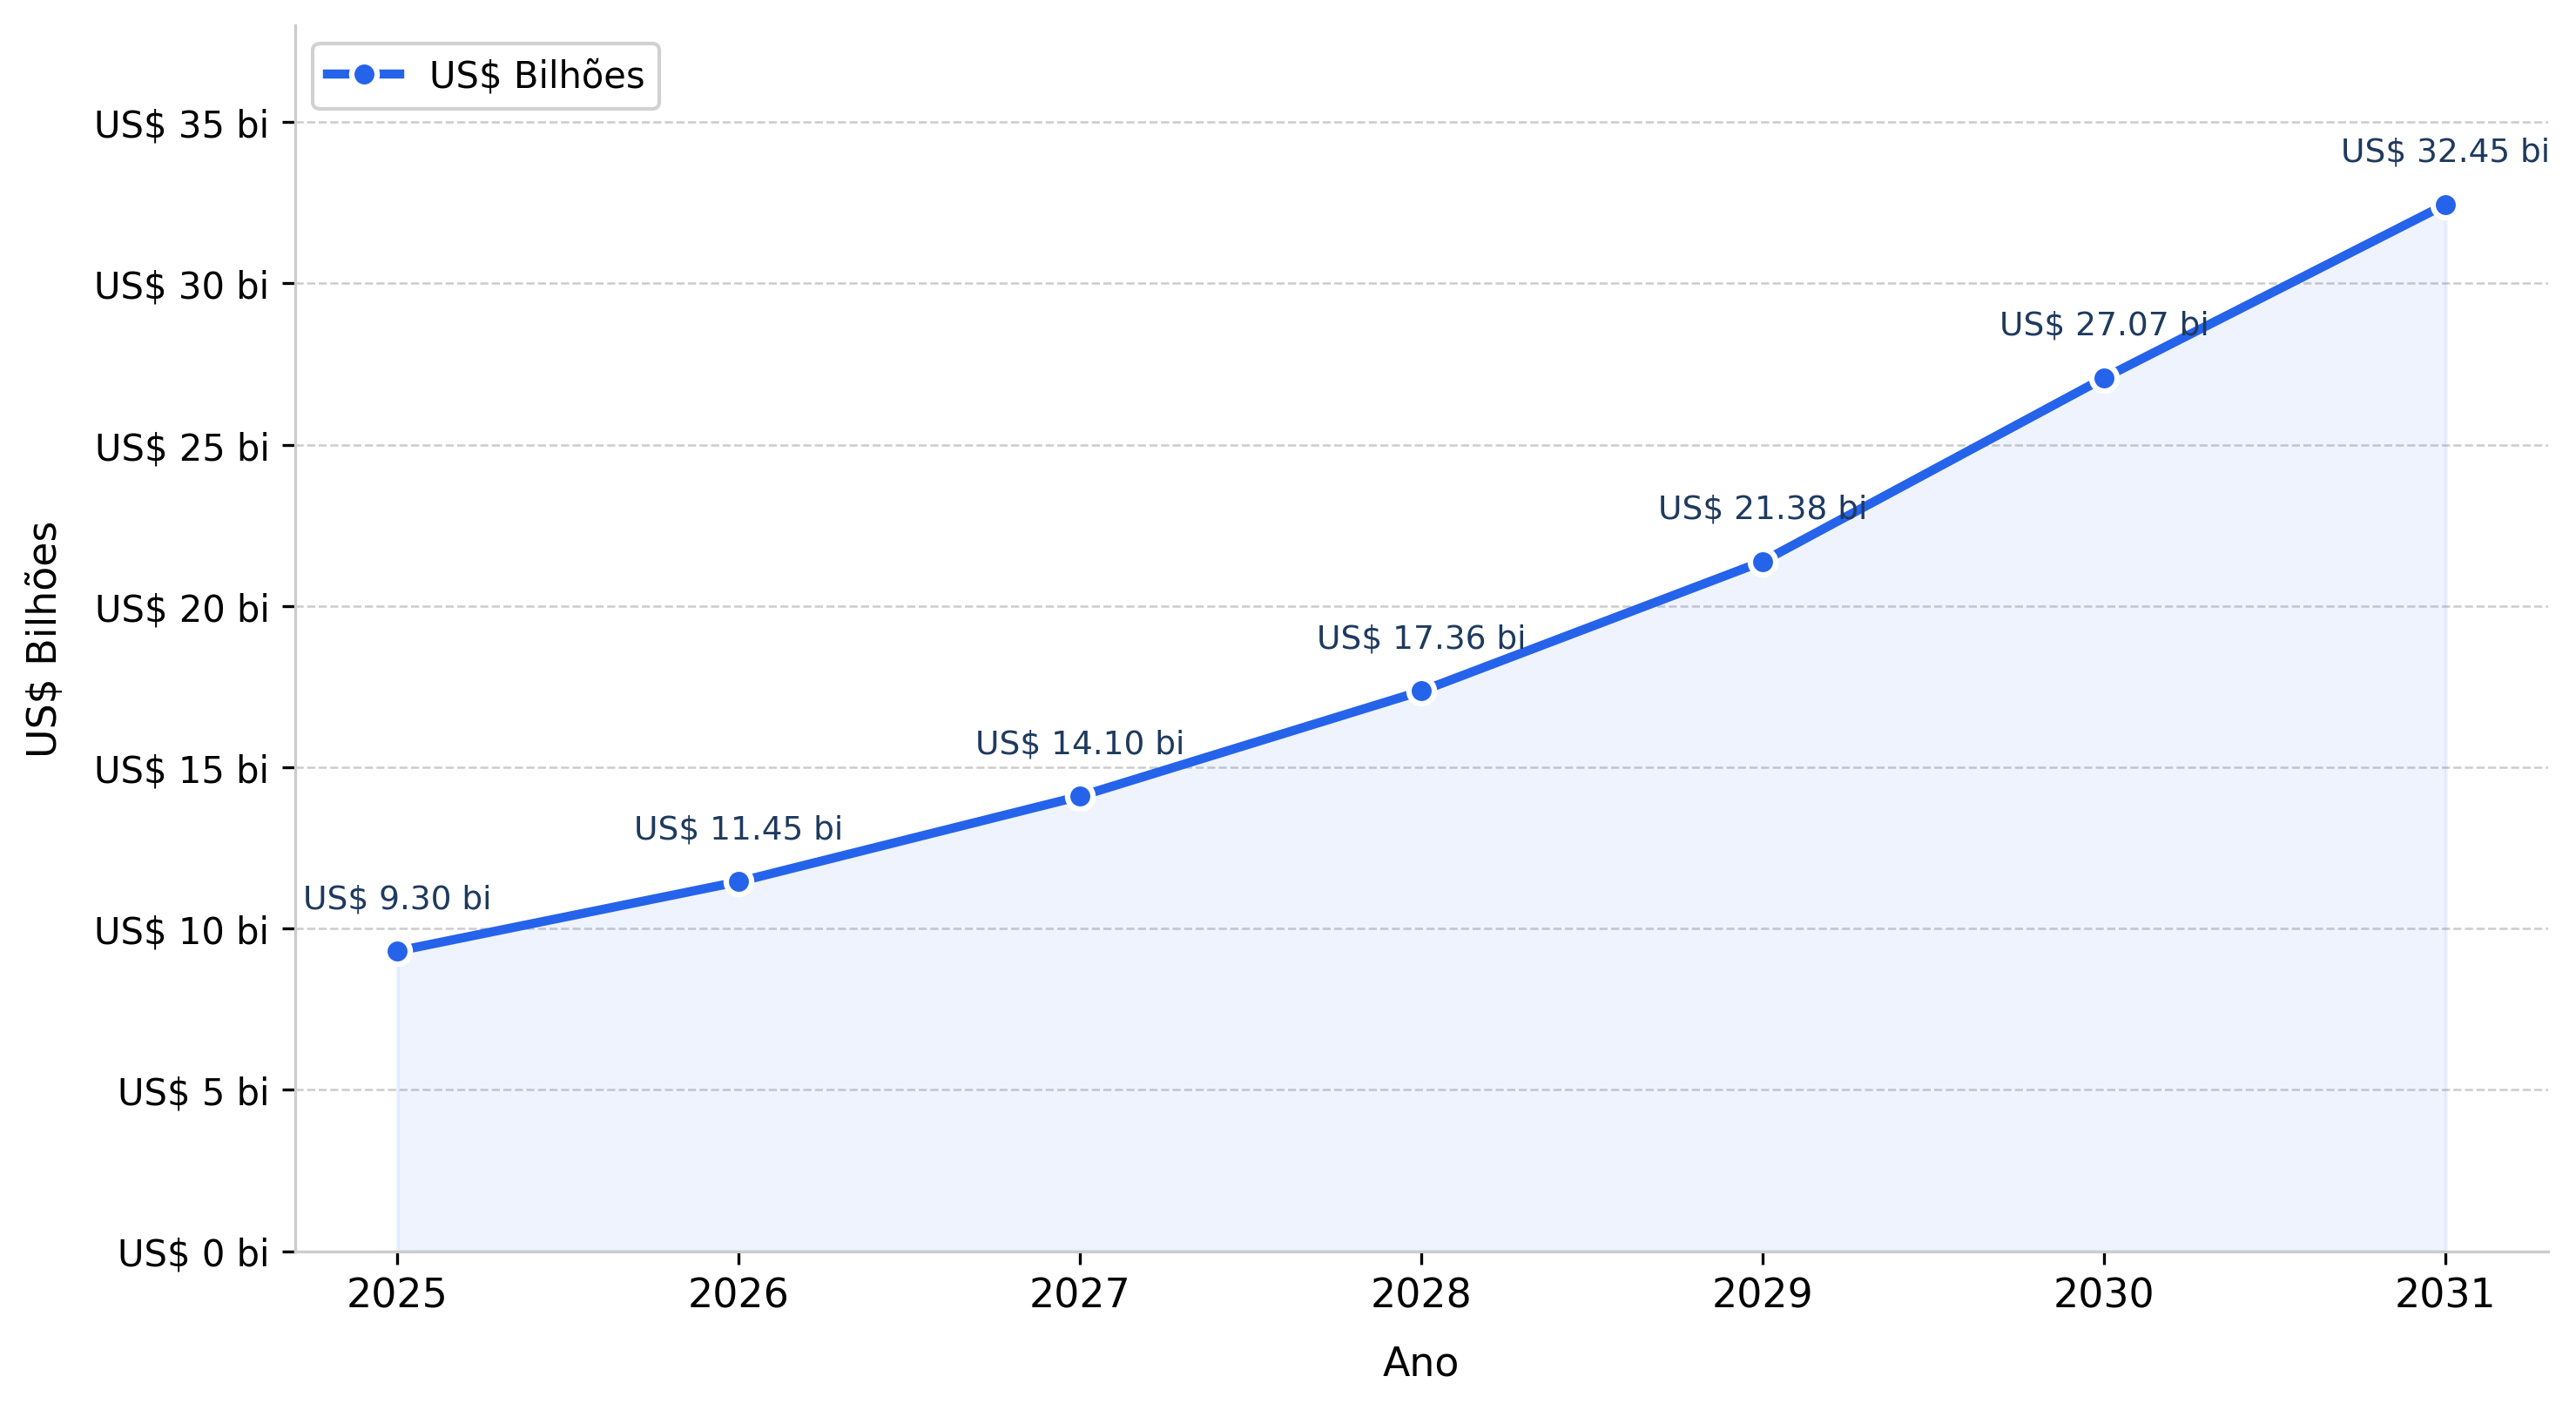
\includegraphics[width=0.9\textwidth]{grafico1_mercado_chatbots.png}
 %   \label{fig:mercado-chatbots}
%
  %  \vspace{0.2cm}
 %   \footnotesize{Fonte: Mordor Intelligence (2026).}\\
%    \footnotesize{Nota: anos intermediários calculados pelo autor com base no CAGR de 23,15\% declarado pela fonte.}
%\end{figure}



\begin{figure}[H]
\centering
\caption{Projeção do mercado global de chatbots}
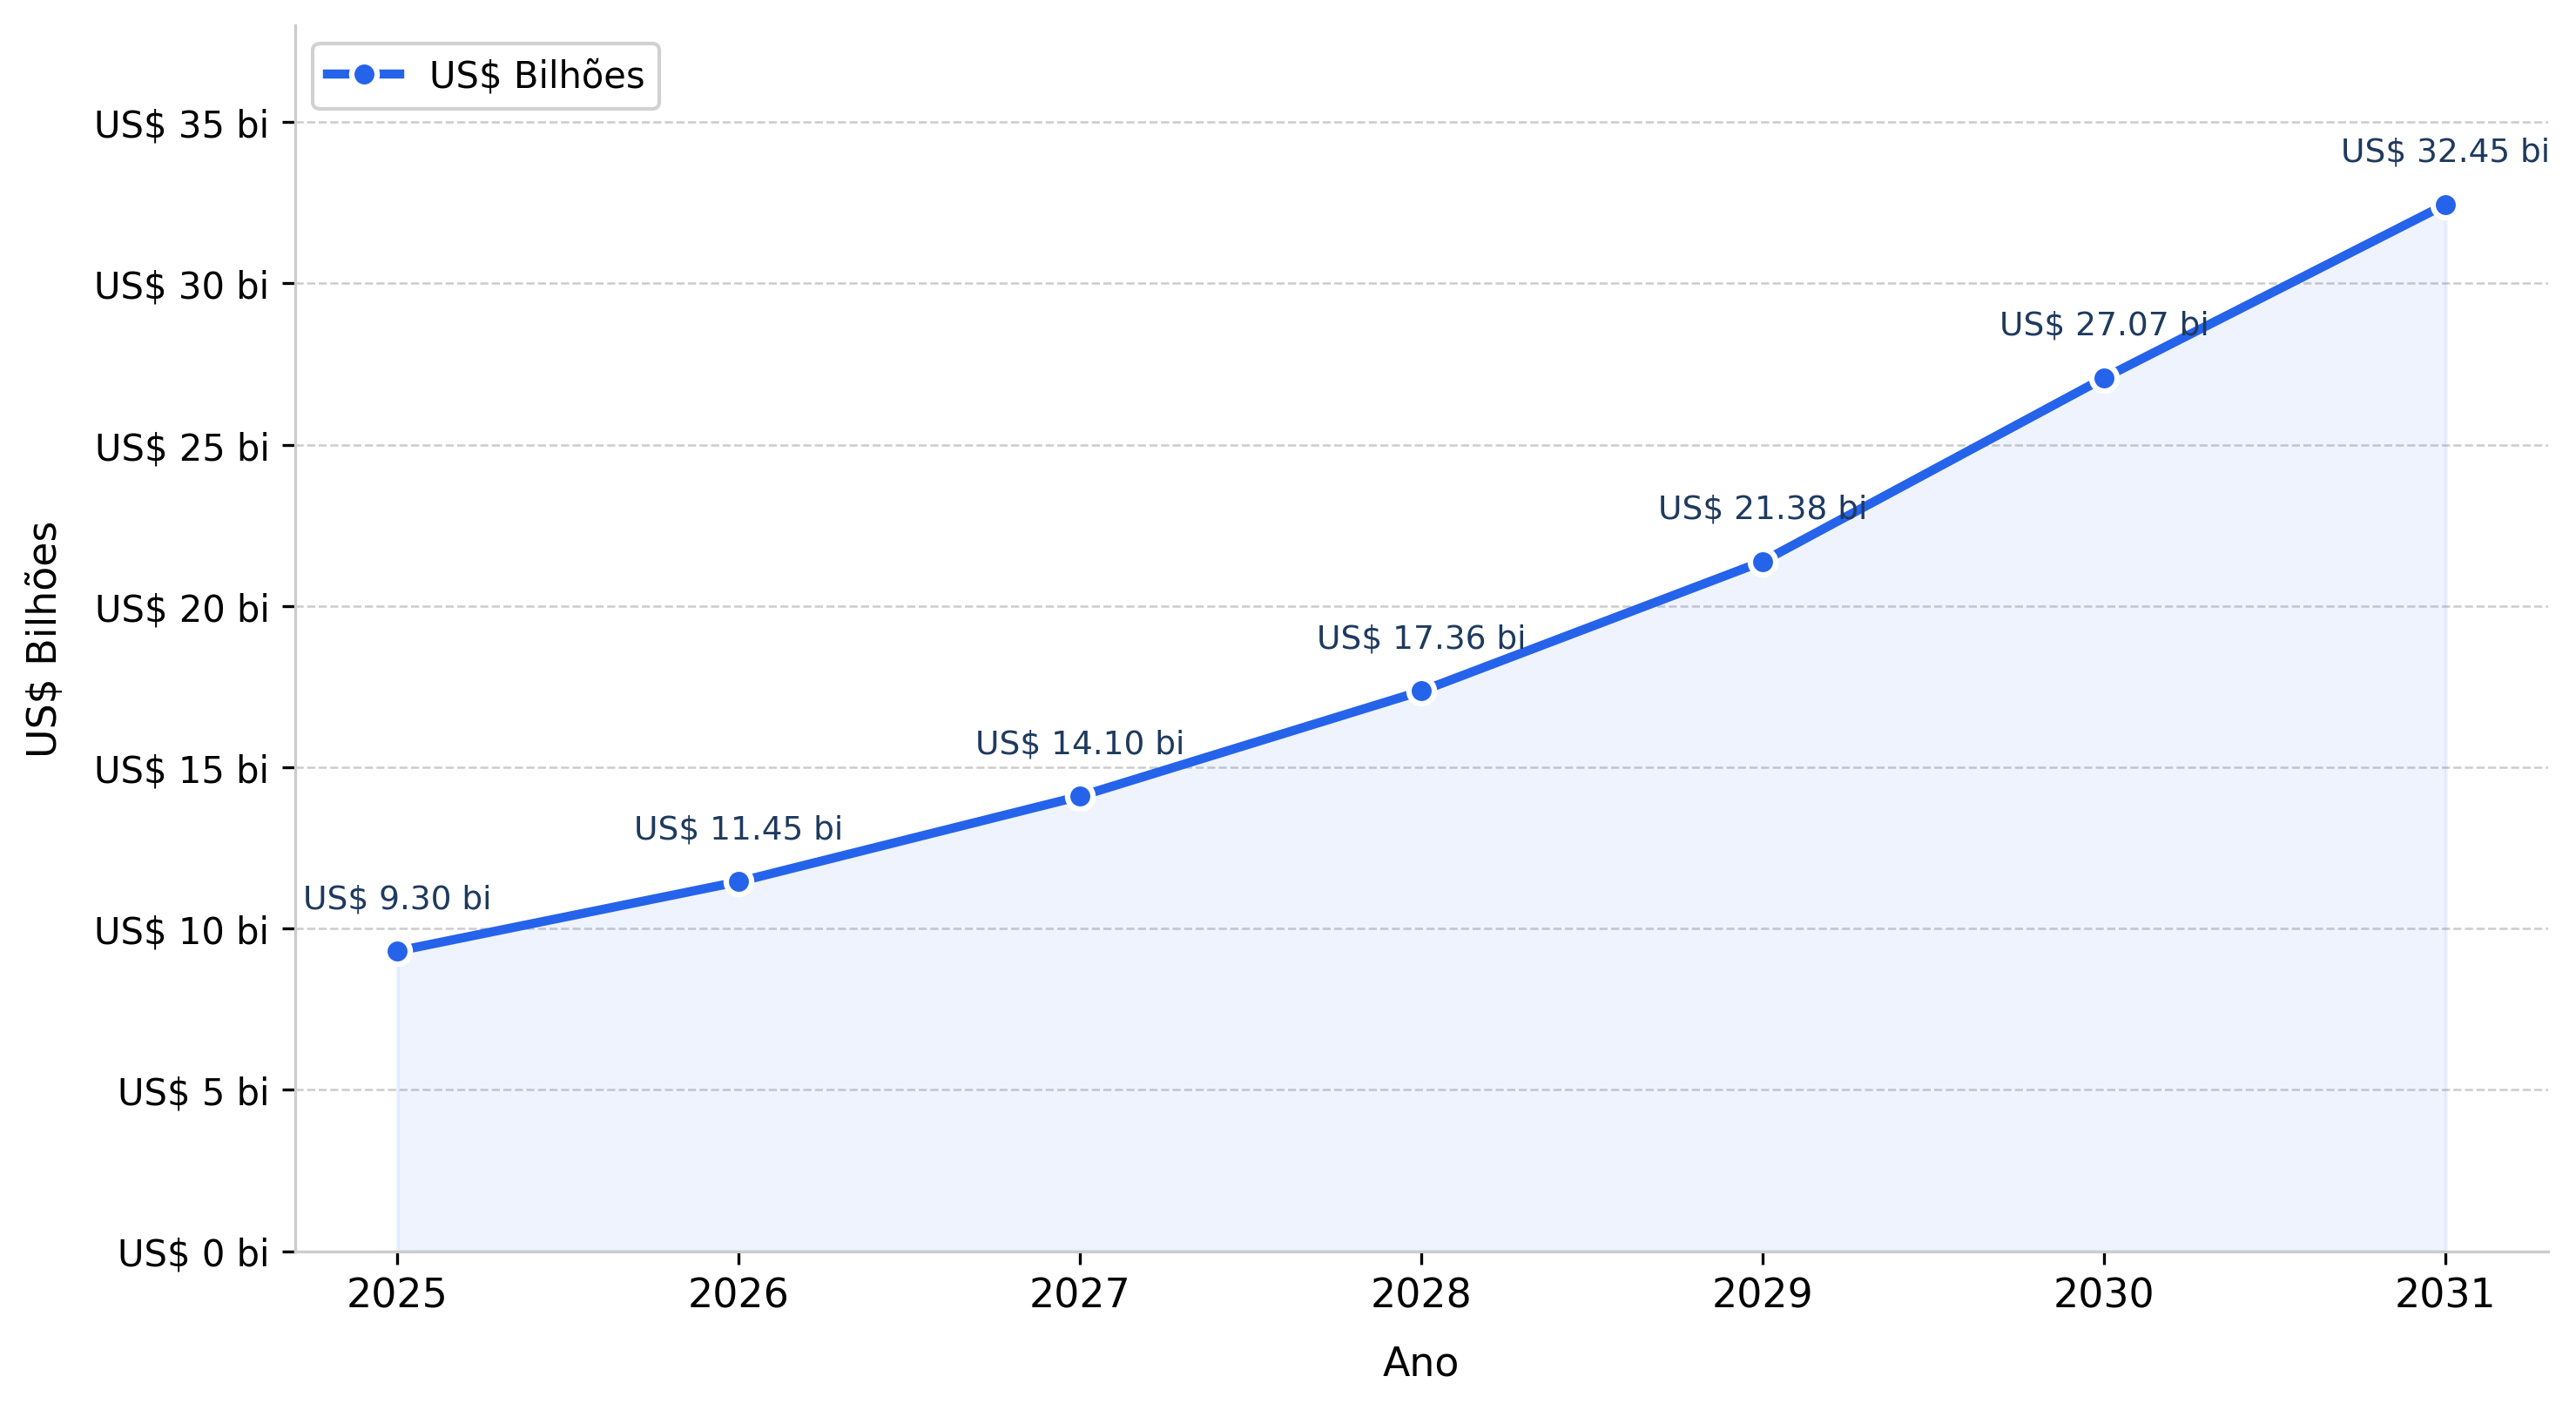
\includegraphics[width=1.0\textwidth]{grafico1_mercado_chatbots.png}
\label{fig:mercado}
\vspace{0.2cm}
\footnotesize{Fonte: Mordor Intelligence (2026).}\\
\footnotesize{Nota: anos intermediários calculados pelo autor com base no CAGR de 23,15\% declarado pela fonte.}
\end{figure}


% TRECHO ANTIGO (revisão pré-banca: repete por extenso a mesma estatística de Li et al.
% (2021) já apresentada na Introdução, com os mesmos números)
%No contexto das clínicas médicas, a relevância dos chatbots é amplificada pelo potencial de redução do tempo de espera e dos custos operacionais. Li et al. (2021), em estudo retrospectivo com 12.342 atendimentos, demonstraram que a introdução de um módulo de triagem assistida por IA reduziu o tempo médio de espera de 1,97 horas para 0,38 horas, resultado estatisticamente significativo que ilustra o impacto operacional de sistemas inteligentes de atendimento. Apesar desse avanço, a literatura ainda carece de soluções específicas para clínicas de pequeno e médio porte que combinem integração a sistemas de agendamento, personalização de respostas via PLN e conformidade com a Lei Geral de Proteção de Dados (LGPD), lacuna que este trabalho busca endereçar.

% TRECHO NOVO
No contexto das clínicas médicas, a relevância dos chatbots é amplificada pelo potencial de redução do tempo de espera, como evidenciado pelo estudo de Li et al. (2021) já apresentado na Introdução, e, possivelmente, dos custos operacionais, aspecto que esse estudo não mediu. Apesar desse avanço, a literatura ainda carece de soluções específicas para clínicas de pequeno e médio porte que combinem integração a sistemas de agendamento, personalização de respostas via PLN e conformidade com a Lei Geral de Proteção de Dados (LGPD), lacuna que este trabalho busca endereçar.

% ------------------------------------------
\subsubsection{Baseado em regras}
\label{sec:regras}
% ------------------------------------------

Nesse tipo de sistema, o chatbot funciona com base em regras pré-definidas. No entanto, quando o padrão de entrada do usuário não corresponde a nenhuma regra programada, o sistema se torna ineficiente, retornando respostas genéricas ou falhando completamente (THORAT; JADHAV, 2020).

Os desenvolvedores utilizam AIML (Artificial Intelligence Markup Language) para codificar essas regras. AIML é uma linguagem baseada em XML, estruturada em \texttt{<category>} com \texttt{<pattern>} (entrada) e \texttt{<template>} (resposta).

THORAT e JADHAV (2020) enfatizam que compor regras para todas as variações possíveis é um trabalho muito árduo: ``marque'' ≠ ``agendar'' ≠ ``consulta amanhã'' exige dezenas de padrões por intenção, tornando a manutenção do sistema progressivamente mais complexa à medida que o escopo de atendimento cresce.

No contexto de uma clínica médica, essa limitação é crítica: pacientes utilizam vocabulários variados para descrever a mesma necessidade, como ``quero marcar'', ``preciso de uma consulta'' ou ``tem horário disponível'', e sistemas baseados em regras falham sistematicamente nessas variações. Caldarini et al. (2022) complementam que sistemas \textit{rule-based} são um ``legado útil'' para finalidades simples, mas que abordagens híbridas com IA são necessárias para resolver a complexidade clínica.

\begin{table}[H]
\centering
\caption{Limitações do Padrão de Correspondência (\textit{Pattern Matching}) em sistemas baseados em regras}
\label{tab:limitacoes-pattern-matching}
\begin{tabular}{p{2.8cm}p{2.2cm}p{7cm}}
\hline
\textbf{Entrada do usuário} & \textbf{O sistema entende?} & \textbf{Causa da falha (Limitação Técnica)} \\
\hline
``Agende a consulta'' & Sim & Corresponde ao padrão programado. \\
``Quero marcar com o Dr.'' & Não & O sistema não reconhece sinônimos (``marcar'' em vez de ``agendar''). \\
``Amanhã 14h Daniel'' & Não & O sistema não consegue separar data, hora e nome sem uma regra específica para essa ordem. \\
\hline
\end{tabular}
\vspace{0.3cm}

\footnotesize{Fonte: Elaborado pelo autor, 2026.}
\end{table}

\textbf{Vantagens dos Rule-Based}
\begin{itemize}
    \item Agilidade no Desenvolvimento de Estruturas Determinísticas: A utilização de sistemas baseados em regras permite uma implementação acelerada para fluxos de conversação lineares e objetivos, como em listas de perguntas frequentes (FAQs), onde as respostas são estáticas e não exigem interpretação contextual profunda;
    \item Consistência e Previsibilidade Operacional: Diferente dos modelos generativos, os sistemas baseados em regras são estritamente determinísticos, o que elimina o risco de ``alucinações'' (geração de informações falsas ou desconexas), garantindo que o chatbot responda exatamente o que foi programado;
    \item Eficiência de Recursos e Ausência de Treinamento: Esses sistemas dispensam o uso de grandes volumes de dados para treinamento e infraestrutura de processamento de alto desempenho, resultando em um custo inicial de computação nulo em comparação ao treinamento de redes neurais complexas.
\end{itemize}

\textbf{Limitações Críticas}
\begin{itemize}
    \item Rigidez Algorítmica: Sistemas baseados em regras apresentam baixa tolerância a variações linguísticas, tornando-se ineficientes quando a entrada do usuário não corresponde exatamente aos padrões predefinidos;
    \item Complexidade de Manutenção: A necessidade de compor regras para cada situação possível gera um esforço de desenvolvimento exaustivo, uma vez que a linguagem AIML exige a escrita manual de regras para múltiplas variações;
    \item Limitação de Escopo Operacional: Esses modelos conseguem processar requisições simples, mas falham em gerenciar fluxos complexos ou de alta demanda, exigindo intervenção humana para solucionar ambiguidades que o sistema não consegue interpretar.
\end{itemize}

% ------------------------------------------
\subsubsection{Baseado em Inteligência Artificial}
\label{sec:ia}
% ------------------------------------------

Os chatbots baseados em Inteligência Artificial diferenciam-se dos sistemas baseados em regras por sua capacidade de aprender com dados e melhorar seu desempenho ao longo do tempo. Esses sistemas utilizam técnicas como Machine Learning e Processamento de Linguagem Natural (PLN) para compreender a intenção do usuário e gerar respostas mais adequadas e contextuais.

Diferentemente dos chatbots tradicionais, que dependem de fluxos fixos, os chatbots baseados em IA são capazes de lidar com variações na linguagem, interpretar perguntas complexas e adaptar-se a diferentes cenários de interação. Segundo Caldarini, Jaf e McGarry (2022), os chatbots modernos utilizam métodos de Inteligência Artificial, especialmente PLN e aprendizado de máquina, para simular conversas humanas e oferecer suporte automatizado mais eficiente.

Esses sistemas funcionam a partir do treinamento com grandes volumes de dados, permitindo identificar padrões de linguagem e prever respostas apropriadas. Além disso, podem evoluir continuamente conforme novas interações são realizadas, tornando-se mais precisos com o uso. Em aplicações mais avançadas, utilizam redes neurais e aprendizado profundo para melhorar a qualidade das respostas e a naturalidade da conversa.

Os chatbots baseados em Inteligência Artificial são capazes de realizar tarefas mais complexas, como classificação de intenções \textit{(intent classification)} e extração de entidades nomeadas \textit{(Named Entity Recognition} -- NER\textit{)}, fundamentais para aplicações como agendamento automatizado. A classificação de intenção consiste em mapear o enunciado do usuário para uma categoria semântica predefinida, como \texttt{agendarConsulta}, \texttt{cancelarConsulta} ou \texttt{informarConvenio}, intenções do protótipo deste trabalho. A extração de entidades, por sua vez, identifica elementos específicos no texto, como, datas, horários, nomes de médicos e especialidades. A combinação dessas duas capacidades permite ao sistema compreender uma frase como ``quero remarcar minha consulta de amanhã com o cardiologista...'' e extrair, simultaneamente, a intenção (\texttt{reagendarConsulta}), a entidade temporal (amanhã) e a especialidade (cardiologia), viabilizando uma resposta precisa e personalizada.

\begin{figure}[H]
    \centering
    \caption{Funcionamento do Classificador de Intenções}
    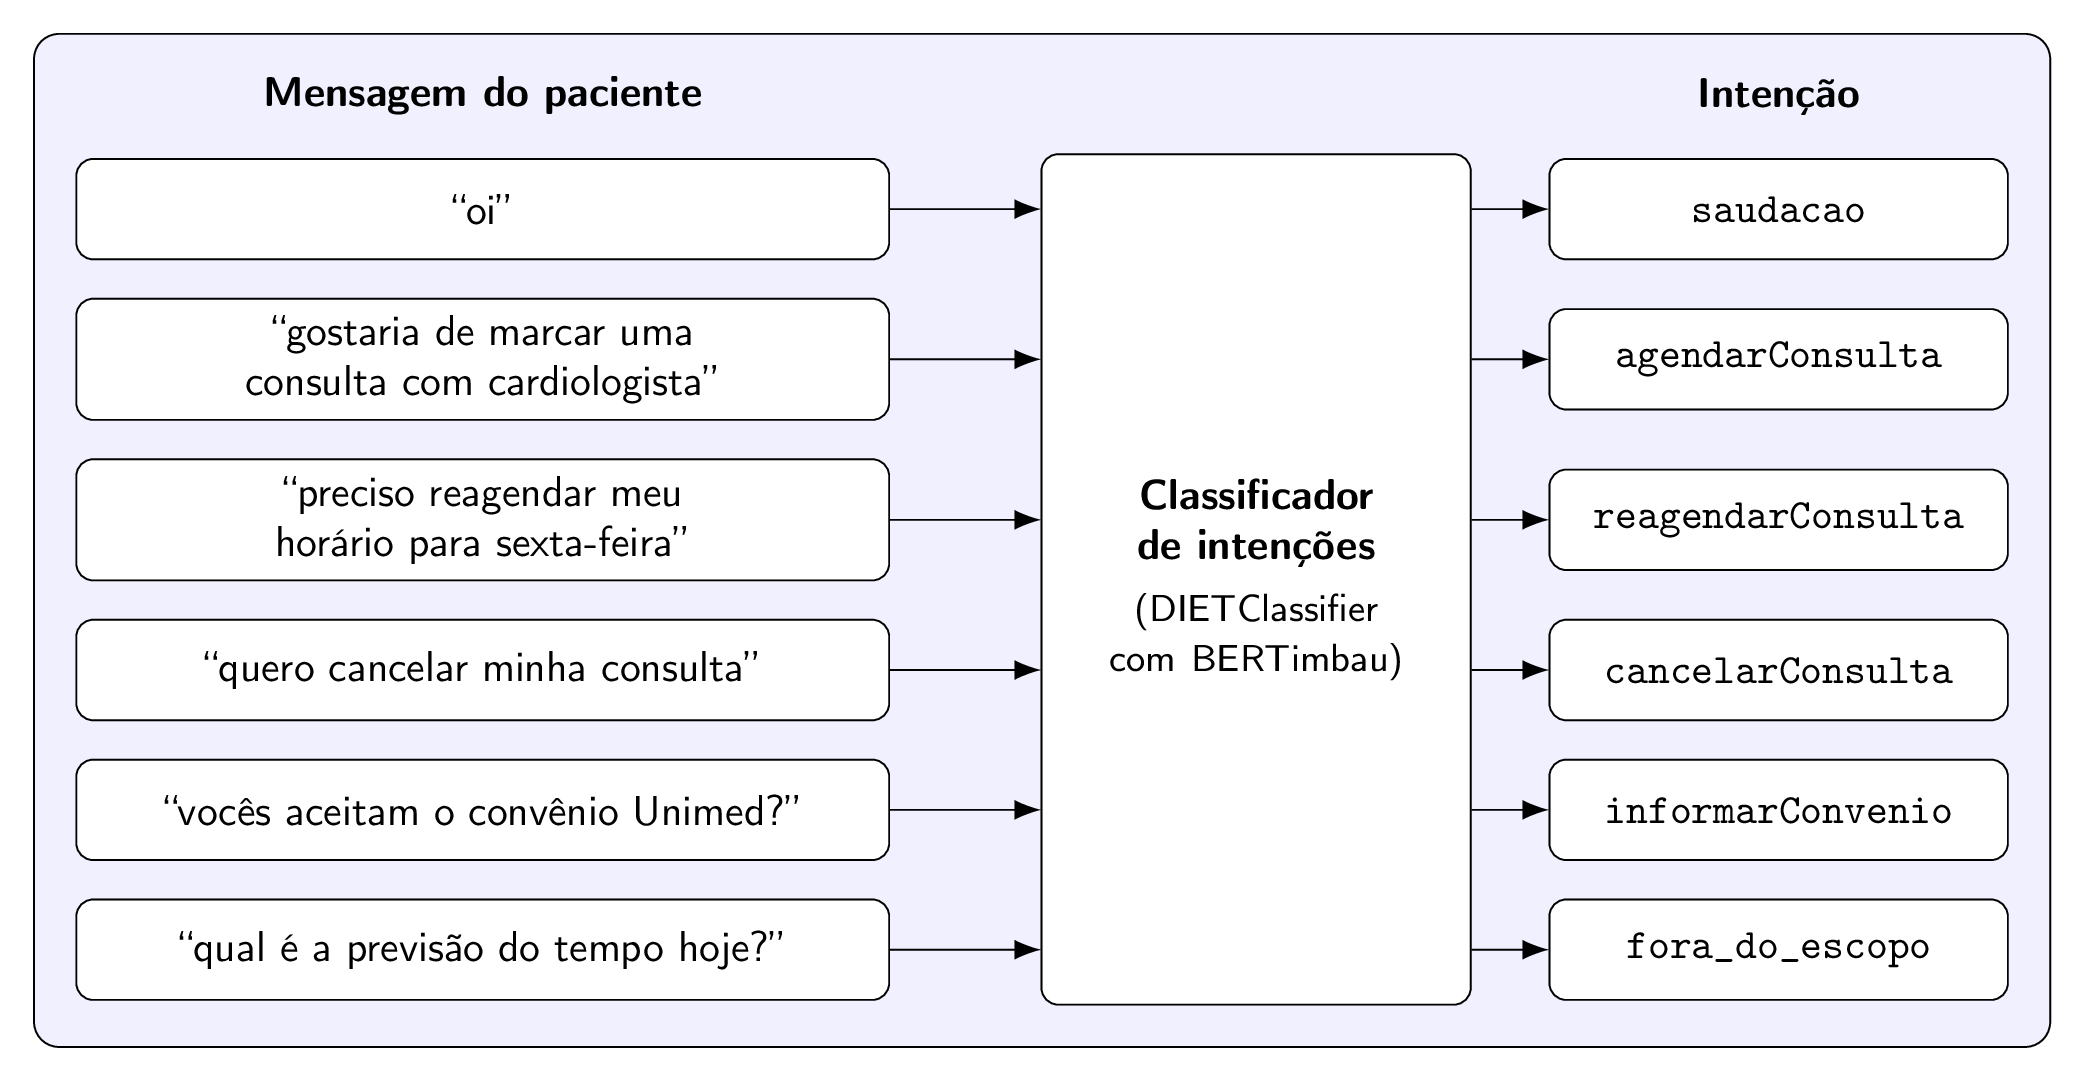
\includegraphics[width=0.95\textwidth]{fig_classificador_intencoes.png}\par
    \label{fig:IntentClass}

    \vspace{0.2cm}
    \footnotesize{Fonte: Elaborado pelo autor, 2026, com frases e intenções do corpus do protótipo.}
\end{figure}


\begin{figure}[H]
    \centering
    \caption{Exemplo de \textit{Named Entity Recognition}}
    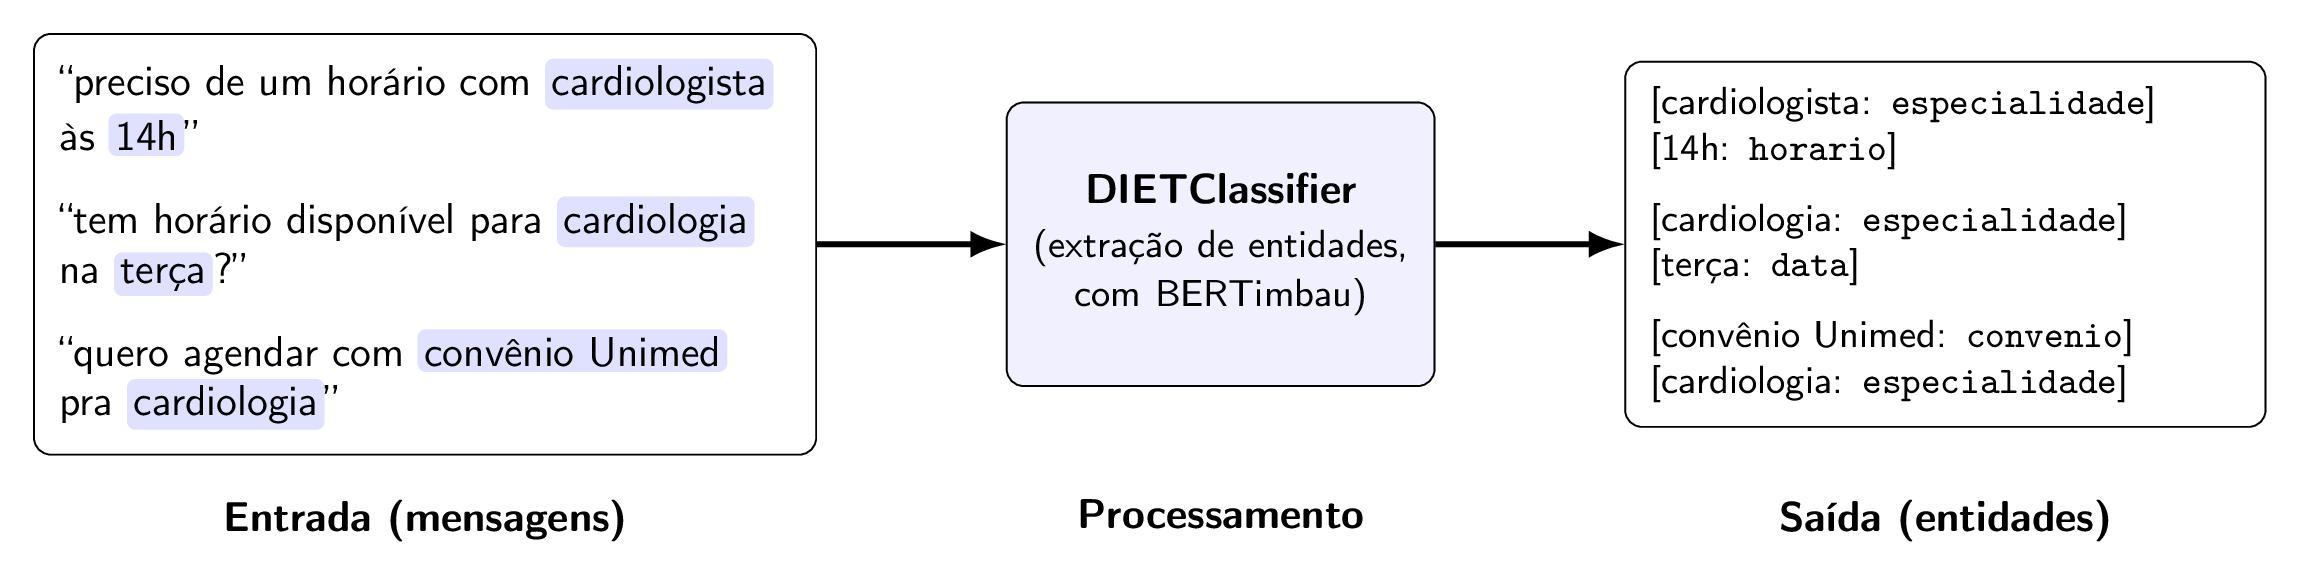
\includegraphics[width=0.95\textwidth]{fig_ner_exemplo.png}\par
    \label{fig:ner}

    \vspace{0.2cm}
    \footnotesize{Fonte: Elaborado pelo autor, 2026, com frases e entidades do corpus do protótipo.}
\end{figure}

No campo dos modelos de linguagem aplicados à saúde, destaca-se o uso de arquiteturas baseadas em BERT (\textit{Bidirectional Encoder Representations from Transformers}), que demonstraram desempenho superior na classificação de textos médicos em comparação a modelos anteriores. Sung, Park e Kim (2023) confirmaram a eficácia do BERT na classificação de dados de aconselhamento em saúde, concluindo que sua capacidade bidirecional de representação contextual o torna particularmente adequado para a compreensão de terminologias médicas variadas. Em clínicas, essas capacidades se traduzem em benefícios concretos: o sistema pode interpretar solicitações variadas como reagendamentos, cancelamentos e dúvidas sobre convênios, adaptando-se ao vocabulário informal dos pacientes sem necessidade de reformulação.

\begin{figure}[H]
    \centering
    \caption{Funcionamento BERT}
    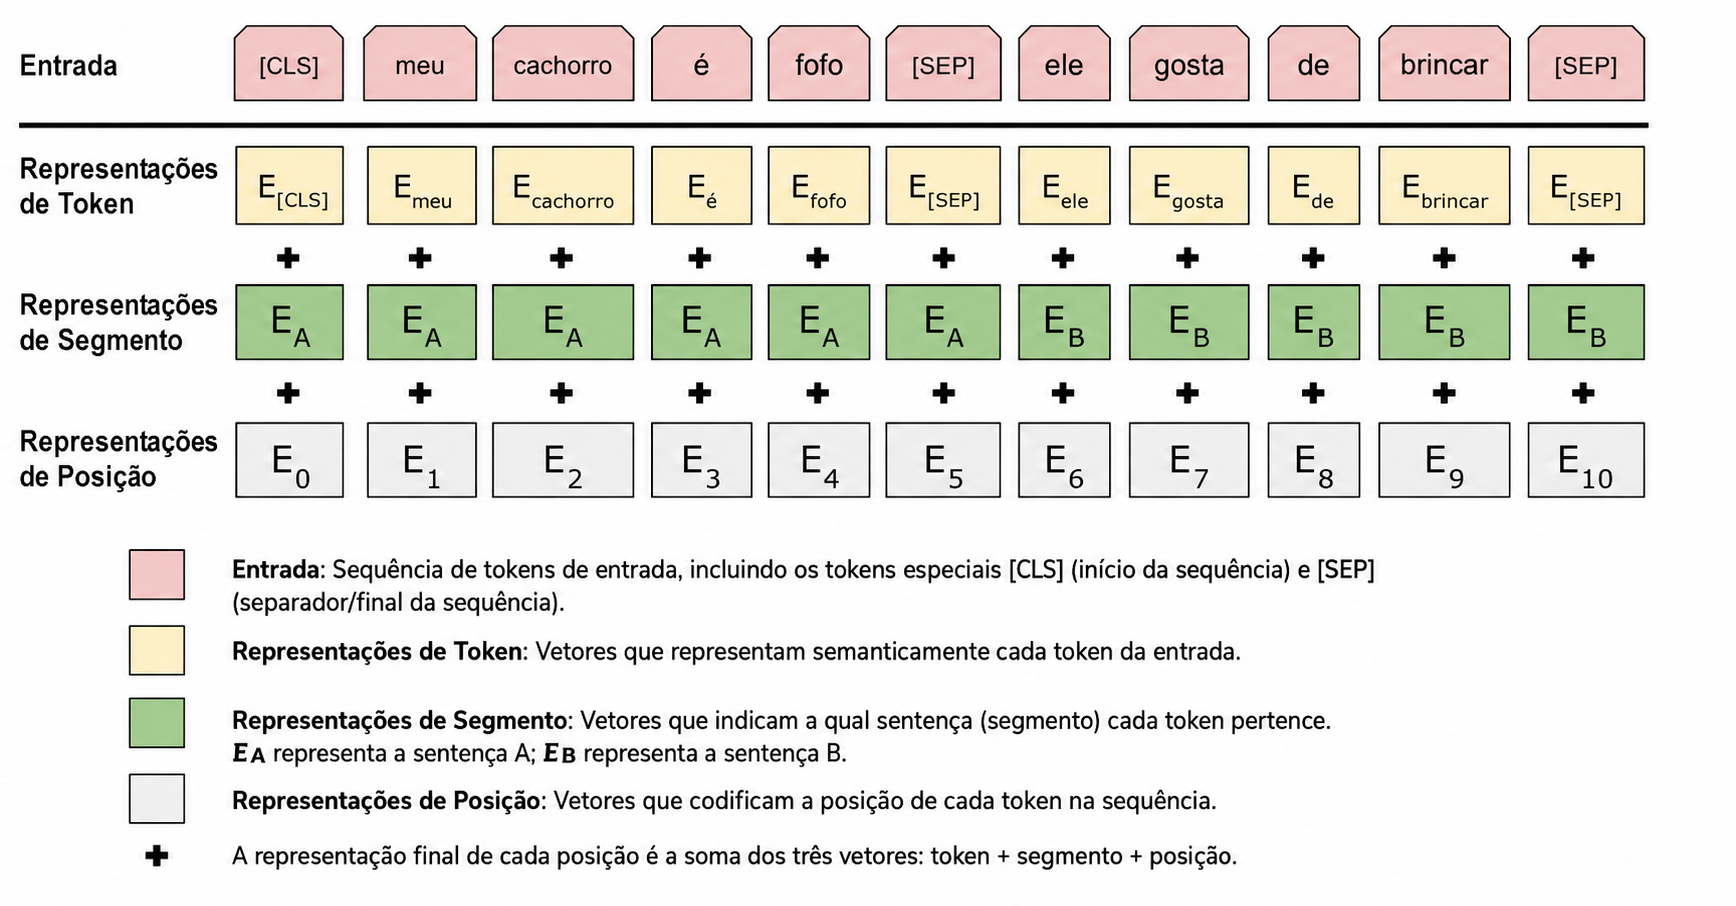
\includegraphics[width=0.9\textwidth]{FuncBert.png}
    \label{fig:FuncBert}

    \vspace{0.2cm}
    \footnotesize{Fonte: Adaptado de Devlin et al. (2019).}\\
\end{figure}


% ------------------------------------------
\subsubsection{Aplicação de Chatbots na área comercial}
% ------------------------------------------

Os chatbots são empregados em diversas áreas, como atendimento ao cliente, educação, comércio eletrônico, saúde, fintech e varejo, entre outras (SIDLAUSKIENE et al., 2023). A Tabela~\ref{tab:chatbot-setores} apresenta as principais áreas de aplicação comercial de chatbots, com suas respectivas funções e embasamento na literatura.

\begin{table}[H]
\centering
\caption{Aplicação de chatbots por setor comercial}
\label{tab:chatbot-setores}

\begin{tabular}{p{3.5cm}p{7cm}p{3.5cm}}
\hline
\textbf{Setor} & \textbf{Aplicação principal} & \textbf{Fonte} \\
\hline
Atendimento ao cliente &
Resolução de dúvidas frequentes, suporte 24/7 e redução do tempo de espera &
Sidlauskiene et al. (2023) \\
Varejo / E-commerce &
Recomendação de produtos, rastreamento de pedidos e recuperação de carrinho abandonado &
Mordor Intelligence (2026) \\
Saúde &
Agendamento de consultas e redução de faltas, com envio de lembretes automáticos &
AlSerkal et al. (2025); Brancewicz et al. (2025) \\
Financeiro (BFSI) &
Consultas bancárias, simulações de crédito e suporte a prevenção de fraudes &
Caldarini et al. (2022) \\
\hline
\end{tabular}

\small Fonte: Elaborado pelo autor com base em Sidlauskiene et al. (2023), Mordor Intelligence (2026), AlSerkal et al. (2025), Brancewicz et al. (2025) e Caldarini et al. (2022).
\end{table}

\subsubsection{Chatbots em Plataformas de Mensageria}

O avanço das tecnologias de comunicação digital contribuiu significativamente para a popularização dos chatbots em plataformas de mensageria. Aplicações como WhatsApp, Telegram, Facebook Messenger e Instagram passaram a ser amplamente utilizadas por empresas e instituições para automatizar atendimentos, fornecer suporte ao cliente e realizar serviços de agendamento de forma rápida e acessível. Nesse contexto, os chatbots tornaram-se ferramentas estratégicas para melhorar a comunicação entre organizações e usuários.

Aplicativos de mensagens instantâneas tornaram-se amplamente utilizados em escala global, especialmente devido à popularização dos dispositivos móveis e da comunicação em tempo real. Segundo dados publicados pela Statista (2026), o WhatsApp ultrapassou a marca de três bilhões de usuários ativos mensais em 2025, consolidando-se como um dos aplicativos de mensageria mais utilizados no mundo. Além disso, plataformas como WeChat, Telegram e Facebook Messenger também apresentam, respectivamente, cerca de 1,41 bilhão, 1 bilhão e 942 milhões de usuários ativos mensais, demonstrando a relevância dos sistemas de comunicação instantânea no cenário atual.

%\begin{figure}[h]
%    \centering
%    \caption{Numero de Usuários de aplicativos de mensagem no mundo}
%  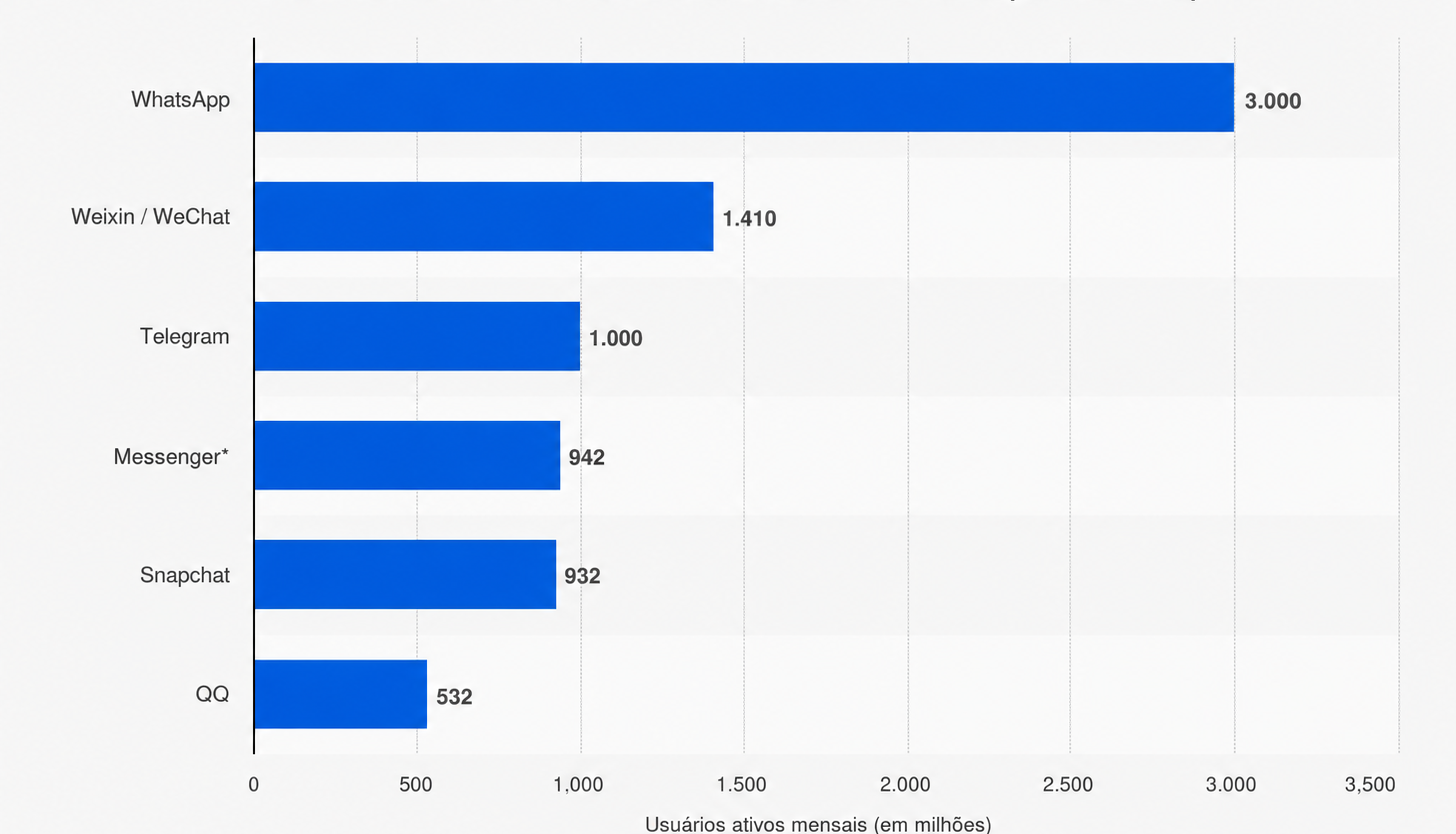
\includegraphics[width=0.9\textwidth]{UsuariosMensagem.png}
%  \label{fig:NumUsu}
%
%    \vspace{0.2cm}
%    \footnotesize{Fonte: Statista (2026).}\\
%\end{figure}

\begin{figure}[H]
\centering
\caption{Número de usuários de aplicativos de mensagem no mundo}
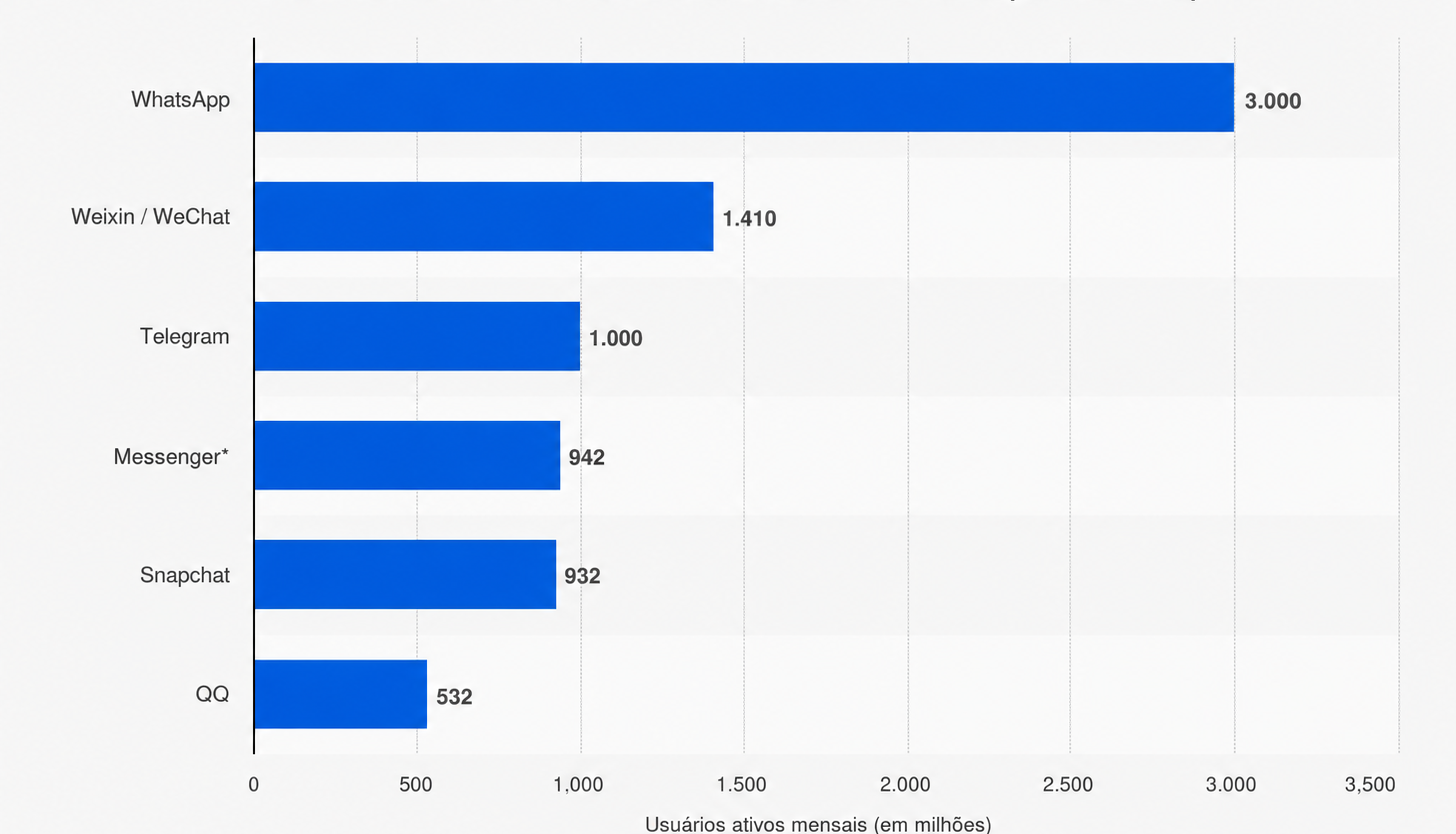
\includegraphics[width=1.0\textwidth]{UsuariosMensagem.png}
\label{fig:mensageria}
\vspace{0.2cm}
\footnotesize{Fonte: Statista (2026).}\\
\end{figure}

Os chatbots em plataformas de mensageria funcionam por meio da integração entre APIs de comunicação e sistemas computacionais responsáveis pelo processamento das mensagens enviadas pelos usuários. As APIs (Application Programming Interfaces) permitem que o chatbot se conecte às plataformas de mensagens, como WhatsApp, Telegram e Facebook Messenger, possibilitando o envio e recebimento automático de mensagens em tempo real.

Quando um usuário envia uma mensagem para o chatbot, a plataforma de mensageria encaminha essa informação para um servidor responsável pelo processamento da conversa. Nesse servidor, o sistema interpreta o conteúdo recebido e identifica a intenção do usuário. Dependendo da arquitetura utilizada (seções~\ref{sec:regras} e~\ref{sec:ia}), essa interpretação pode ocorrer de maneira simples, por meio de regras pré-definidas, ou utilizando técnicas de Inteligência Artificial e Processamento de Linguagem Natural (PLN), capazes de compreender a linguagem humana de forma mais avançada.

Após interpretar a solicitação do usuário, o chatbot executa uma ação correspondente. Em sistemas de agendamento médico, por exemplo, o chatbot pode consultar bancos de dados, verificar horários disponíveis, registrar consultas e enviar confirmações automaticamente. Essas operações geralmente são realizadas por meio da integração com sistemas externos, APIs REST e bancos de dados responsáveis pelo armazenamento das informações.

A utilização dessas integrações proporciona maior automação dos serviços, redução do tempo de atendimento e disponibilidade contínua aos usuários, sendo amplamente aplicada em setores como comércio eletrônico, suporte técnico e serviços de saúde.
% ------------------------------------------
\subsection{Inteligência Artificial}
% ------------------------------------------

A Inteligência Artificial (IA) refere-se à simulação da inteligência humana por um sistema ou máquina. O objetivo da IA é desenvolver uma máquina capaz de pensar como humanos e imitar comportamentos humanos, incluindo percepção, raciocínio, aprendizado, planejamento, previsão e assim por diante (XU et al., 2021).

O início da pesquisa moderna em IA remonta a John McCarthy, que cunhou o termo ``inteligência artificial (IA)'' durante uma conferência no Dartmouth College em 1956. Isso simbolizou o nascimento do campo científico da IA (McCARTHY et al., 1955; XU et al., 2021). Com o passar dos anos, a área evoluiu bastante, passando por diferentes fases, indo de sistemas simbólicos até abordagens atuais baseadas em dados.

Uma das classificações mais conhecidas da área de Inteligência Artificial é a IA fraca e IA forte, propostas por Searle em 1980. A Inteligência Artificial fraca diz respeito a sistemas projetados para executar tarefas específicas, simulando comportamentos inteligentes sem possuir consciência ou entendimento real. Já a Inteligência Artificial forte diz respeito à hipótese de que máquinas podem desenvolver consciência, compreensão e estados mentais equivalentes aos humanos (SEARLE, 1980; RUSSELL; NORVIG, 2021). Para os fins deste trabalho, o foco recai sobre a IA fraca aplicada, especificamente nos sistemas de aprendizado de máquina e PLN que viabilizam os chatbots inteligentes.

Também há diferentes tipos de abordagens a respeito de como a IA ``aprende'', destacam-se o aprendizado de máquina (Machine Learning) e o aprendizado profundo (Deep Learning). Machine Learning é um campo da inteligência artificial que se concentra no desenvolvimento de algoritmos capazes de aprender a partir de dados e experiências, sem a necessidade de programação explícita para cada tarefa. Esses algoritmos são projetados para identificar padrões e tomar decisões com base nas informações fornecidas. Já o Deep Learning é uma subárea da aprendizagem de máquina que permite aos sistemas aprender diretamente a partir de dados brutos, utilizando redes neurais artificiais com múltiplas camadas, eliminando a necessidade de extração manual de características (EL NAQA; MURPHY, 2022).

Uma distinção conceitual adicional, essencial para a compreensão crítica dos sistemas modernos, é a diferença entre IA simbólica e IA conexionista. A IA simbólica representa o conhecimento por meio de símbolos e regras lógicas explícitas, operando de forma transparente e interpretável, porém com baixa tolerância à variabilidade e ao ruído dos dados. A IA conexionista, em contraste, aprende representações implicitamente a partir de grandes volumes de dados por meio de redes neurais, o que confere maior capacidade de generalização, mas impõe desafios de interpretabilidade e pode introduzir vieses presentes nos dados de treinamento (RUSSELL; NORVIG, 2021; GOODFELLOW; BENGIO; COURVILLE, 2016). Essa distinção é relevante para o contexto clínico, onde a explicabilidade das decisões do sistema é um requisito ético e regulatório importante.

\begin{figure}[H]
    \centering
    \caption{IA Simbólica e IA Conexionista}
    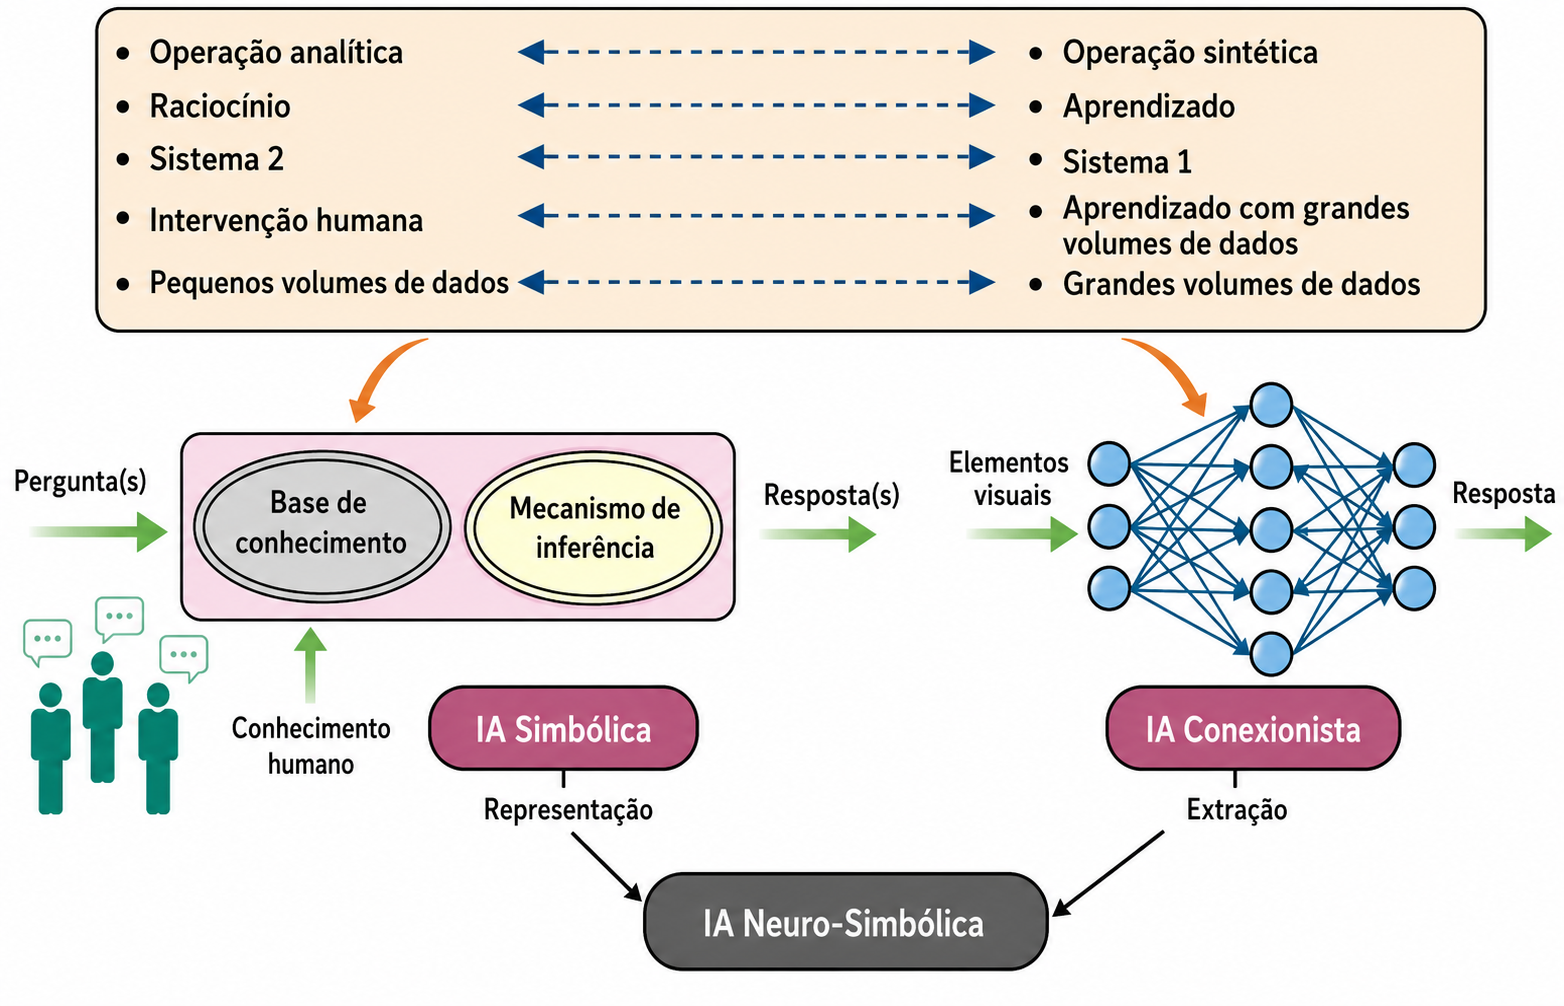
\includegraphics[width=0.85\textwidth]{IaConexionistaIaSimbolica.png}
    \label{fig:ia-cx-sb}

    \vspace{0.2cm}
    \footnotesize{Fonte: Adaptado de Hassan(2022)}
\end{figure}

Especificamente no que diz respeito aos modelos de linguagem de larga escala (Large Language Models -- LLMs), uma limitação crítica amplamente documentada na literatura é o fenômeno das alucinações: a geração de informações plausíveis, mas incorretas ou inteiramente inventadas pelo próprio modelo. Roustan e Bastardot (2025) alertam que as implicações para a prática clínica incluem desde a geração de informações diagnósticas e terapêuticas imprecisas até o reforço de raciocínios diagnósticos errados, além da falta de confiabilidade quando utilizados sem supervisão adequada. No contexto de um chatbot para clínicas, esse risco justifica a adoção de arquiteturas controladas com fluxos de decisão delimitados, em oposição ao uso irrestrito de LLMs generativos, especialmente para funções que envolvem dados sensíveis de saúde.

\begin{figure}[H]
    \centering
    \caption{Relação entre Inteligência Artificial, Machine Learning e Deep Learning}
    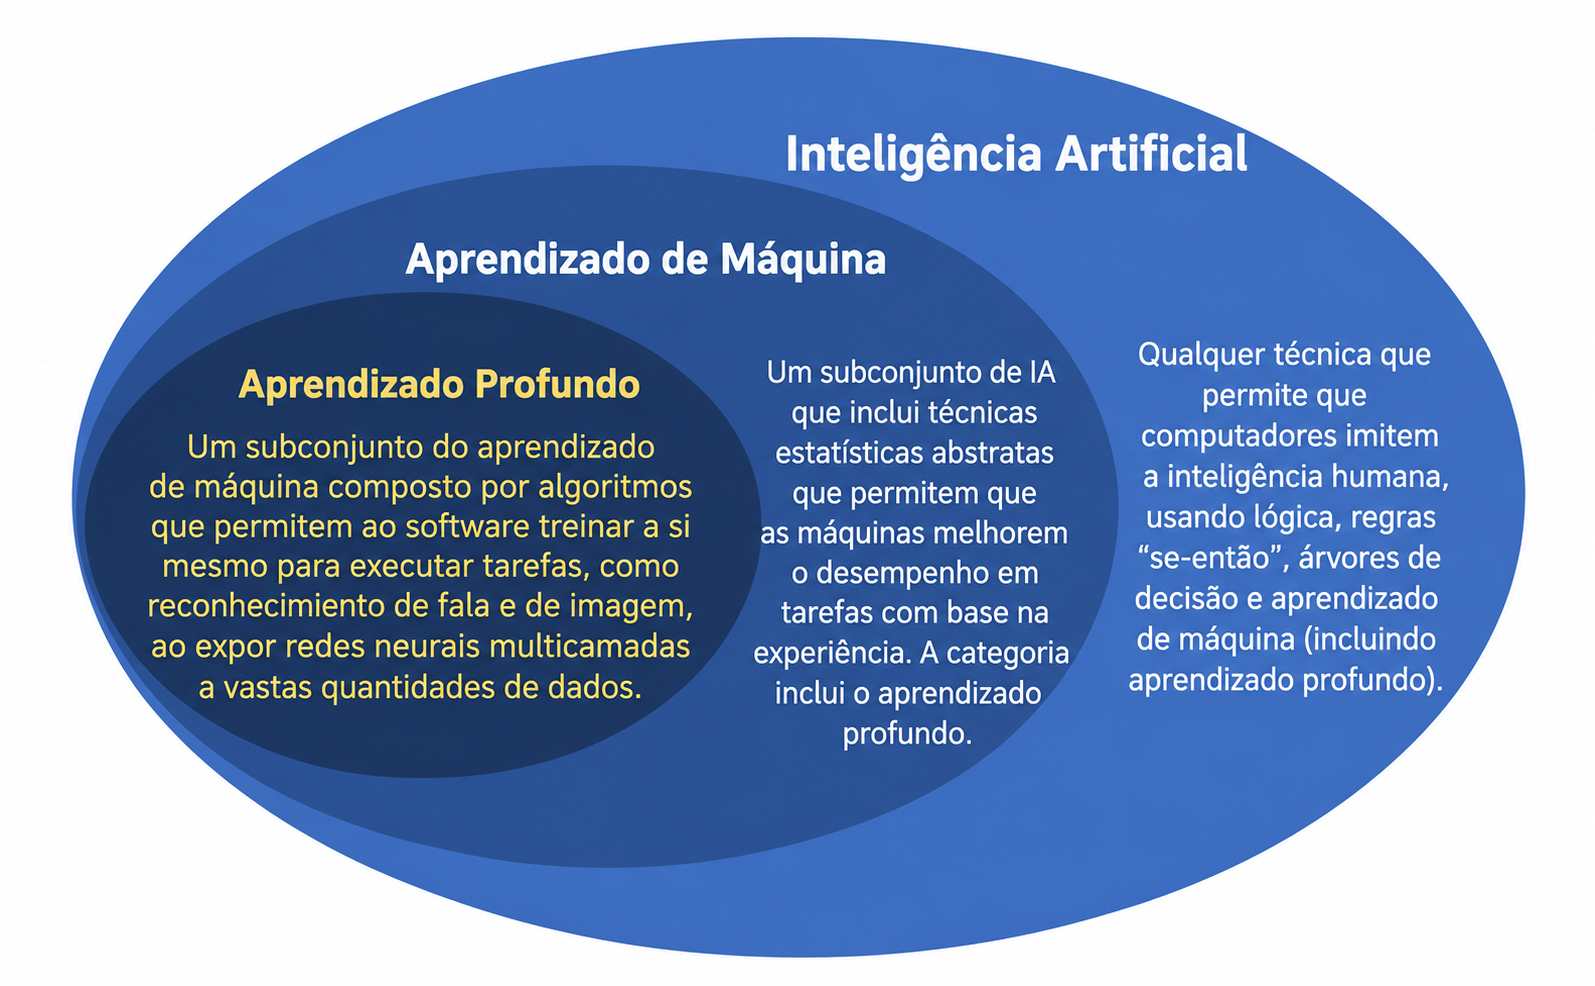
\includegraphics[width=0.85\textwidth]{IaMlDl.png}
    \label{fig:ia-ml-dl}

    \vspace{0.2cm}
    \footnotesize{Fonte: Adaptado de Sajid (2026).}
\end{figure}

% ------------------------------------------
\subsection{Processamento de Linguagem Natural (PLN)}
\label{sec:pln}
% ------------------------------------------

O Processamento de Linguagem Natural (PLN) é uma subárea da inteligência artificial que se dedica ao desenvolvimento de técnicas e métodos que permitem aos computadores compreender, interpretar e gerar linguagem humana (JURAFSKY; MARTIN, 2023).

O PLN combina conceitos de linguística, ciência da computação e inteligência artificial para possibilitar a interação entre humanos e máquinas de forma mais natural. Entre suas aplicações mais comuns estão tradutores automáticos, assistentes virtuais, sistemas de recomendação e chatbots.

O processamento da linguagem natural envolve diversas etapas, entre as quais se destacam a tokenização, que consiste na divisão do texto em unidades menores (tokens), a análise sintática, responsável por identificar a estrutura gramatical das frases, e a análise semântica, que busca compreender o significado das palavras no contexto em que estão inseridas (JURAFSKY; MARTIN, 2023).

Essas etapas são fundamentais para o funcionamento de sistemas conversacionais, pois permitem que o chatbot compreenda corretamente as intenções dos usuários e responda de forma coerente. No entanto, o PLN ainda enfrenta desafios relevantes, como a ambiguidade da linguagem, o uso de expressões informais e a necessidade de interpretação contextual, fatores que podem impactar a precisão das respostas geradas pelos sistemas (JURAFSKY; MARTIN, 2023).

Uma inovação no PLN moderno é o uso de \textit{embeddings}: representações vetoriais densas que codificam o significado semântico das palavras em espaços de alta dimensionalidade. Mikolov et al. (2013) introduziram o Word2Vec, modelo neural que aprende representações de palavras com base em sua distribuição contextual em grandes corpora textuais. O princípio é direto: palavras que aparecem em contextos semelhantes possuem significados próximos e, portanto, vetores próximos no espaço de \textit{embeddings}, propriedade que viabiliza a similaridade semântica computacional. Uma extensão relevante é o GloVe (\textit{Global Vectors for Word Representation}), proposto por Pennington, Socher e Manning (2014), que combina estatísticas locais de co-ocorrência com informações globais do corpus para gerar representações vetoriais mais ricas semanticamente.

No entanto, tanto o Word2Vec quanto o GloVe produzem representações estáticas, ou seja, a mesma palavra recebe o mesmo vetor independentemente do contexto em que aparece. Essa limitação foi superada pelos modelos contextuais, especialmente o BERT (\textit{Bidirectional Encoder Representations from Transformers}), desenvolvido por Devlin et al. (2019). O BERT gera representações dinâmicas: o vetor de uma palavra é calculado em função do contexto completo da sentença, capturando diferenças como multiplicidade de sentidos e dependências sintáticas de longo alcance. Essa capacidade bidirecional o torna especialmente eficaz para tarefas como classificação de intenção e extração de entidades em sistemas conversacionais para saúde, onde a precisão semântica é crítica (SUNG; PARK; KIM, 2023).

\begin{figure}[H]
    \centering
    \caption{Como funcionam: GloVe, BERT, Word2Vec}
    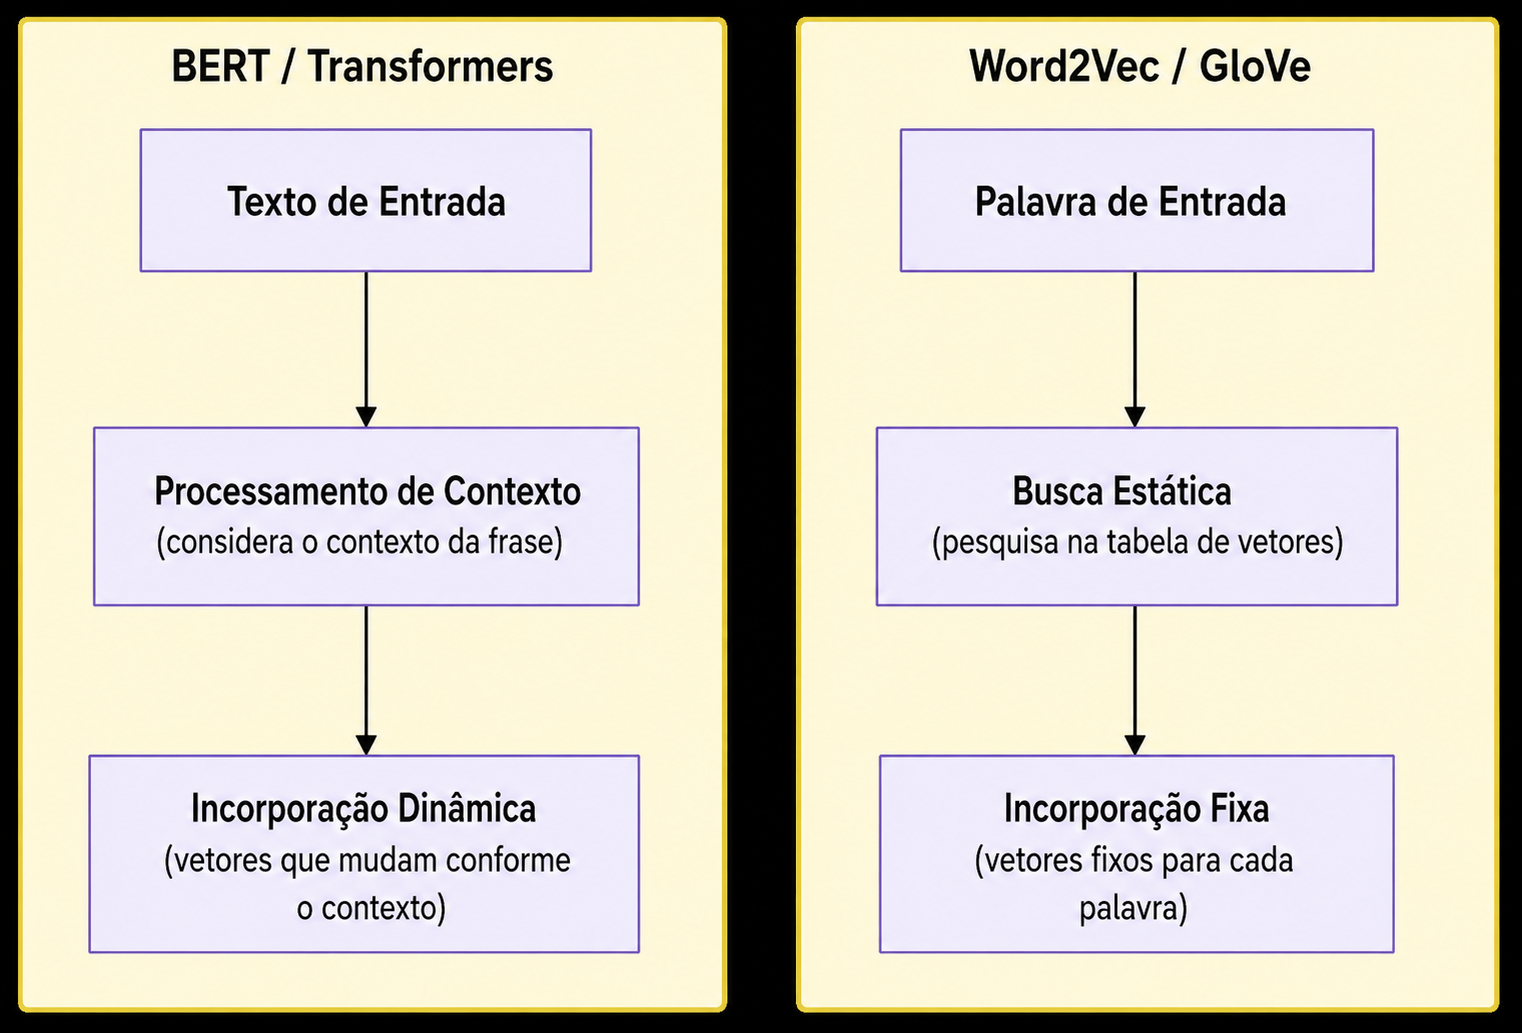
\includegraphics[width=0.85\textwidth]{GloveBertWord.png}
    \label{fig:gl-bt-wd}

    \vspace{0.2cm}
    \footnotesize{Fonte: Adaptado de Harsoor(2024)}
\end{figure}

Para ilustrar a importância do PLN no contexto deste trabalho, considere a seguinte frase: ``quero remarcar minha consulta de amanhã com o cardiologista''. Um sistema de PLN bem configurado deve extrair os seguintes itens: 

\begin{itemize}
    \item A intenção \texttt{reagendarConsulta};
    \item A entidade temporal \texttt{data}, \textit{amanhã};
    \item A entidade \texttt{especialidade}, \textit{cardiologista}, associada à Cardiologia.
\end{itemize}

Esse processo de extração simultânea de intenção e entidades é a base do \textit{pipeline} de compreensão de linguagem natural (NLU) que alimenta o chatbot proposto neste projeto.

A resolução dessas ambiguidades exige modelos capazes de manter representações do contexto conversacional ao longo de múltiplos turnos, um requisito que os modelos baseados em Transformers atendem de forma mais eficaz do que as arquiteturas recorrentes anteriores (JURAFSKY; MARTIN, 2023).

% ------------------------------------------
\subsection{Arquiteturas e Frameworks para Desenvolvimento do Chatbot}
% ------------------------------------------

A implementação de um chatbot baseado em PLN exige decisões técnicas fundamentadas sobre a arquitetura de modelos de linguagem e sobre os frameworks de desenvolvimento a serem utilizados. Esta seção apresenta os fundamentos técnicos dessas escolhas, articulando-os diretamente com os requisitos do sistema proposto neste trabalho.

\subsubsection{A Arquitetura Transformer}

% TRECHO ANTIGO (revisão pré-banca: explicação didática muito próxima da forma como
% a literatura de referência descreve o Transformer, sem análise crítica adicional
% ligada ao caso de uso do trabalho)
%A base técnica dos modelos de PLN modernos é a arquitetura Transformer, introduzida por Vaswani et al. (2017) no artigo \textit{``Attention Is All You Need''}. Antes dessa proposta, os modelos dominantes para processamento sequencial de linguagem eram as Redes Neurais Recorrentes (RNNs) e suas variantes, como as LSTMs (\textit{Long Short-Term Memory}). Essas arquiteturas processavam sequências palavra por palavra, de forma linear, o que criava dois problemas estruturais: a dificuldade de capturar dependências de longo alcance (palavras distantes entre si na sentença) e a impossibilidade de paralelização do treinamento, já que cada estado dependia do anterior.
%
%O Transformer resolveu ambos os problemas por meio de um mecanismo denominado \textit{self-attention} (atenção própria), que permite ao modelo calcular, para cada palavra da sequência, uma pontuação de relevância em relação a todas as outras palavras simultaneamente, independentemente da distância entre elas. Matematicamente, o mecanismo de atenção é definido como:

% TRECHO NOVO
Os modelos de PLN adotados neste trabalho: BERT e, por extensão, o BERTimbau, têm como base a arquitetura Transformer, proposta por Vaswani et al. (2017). Essa escolha arquitetural não é incidental: modelos anteriores, como as Redes Neurais Recorrentes (RNNs) e suas variantes LSTM (\textit{Long Short-Term Memory}), processam a sentença palavra por palavra em sequência, o que impõe duas restrições relevantes ao caso de uso deste trabalho. Primeiro, torna mais difícil relacionar palavras distantes entre si na mesma frase, por exemplo, associar corretamente ``cardiologista'' à intenção de reagendamento quando outras palavras aparecem entre os dois termos. Segundo, impede a paralelização do treinamento, já que cada palavra só pode ser processada depois da anterior, tornando o treinamento de modelos em português, com corpora menores que os do inglês, mais custoso.

O Transformer contorna essas duas limitações por meio do mecanismo de \textit{self-attention}: em vez de processar a sentença em sequência, o modelo calcula, para cada palavra, sua relevância em relação a todas as demais palavras da sentença simultaneamente. Isso é o que permite ao BERTimbau, por exemplo, relacionar uma entidade temporal a uma especialidade médica mesmo quando elas estão distantes na frase do paciente. Formalmente, esse mecanismo é expresso como:

\begin{equation}
\text{Attention}(Q, K, V)=
\text{softmax}\left(
\frac{QK^T}{\sqrt{d_k}}
\right)V
\label{eq:attention}
\end{equation}

\myequation{Mecanismo de Atenção do Transformer}

% TRECHO ANTIGO
%onde $Q$ (queries), $K$ (keys) e $V$ (values) são projeções lineares da entrada, e $d_k$ é a dimensão das chaves. Em sua formulação de \textit{multi-head attention}, o modelo aplica esse mecanismo em paralelo com diferentes projeções aprendidas, capturando relações semânticas e sintáticas em diferentes subespaços representacionais (VASWANI et al., 2017). Essa capacidade de processamento paralelo reduziu drasticamente o tempo de treinamento e melhorou a qualidade das representações, estabelecendo o Transformer como a arquitetura base de praticamente todos os modelos de linguagem modernos, incluindo o BERT, o GPT e seus sucessores.

% TRECHO NOVO
onde $Q$ (\textit{queries}), $K$ (\textit{keys}) e $V$ (\textit{values}) são projeções lineares da sentença de entrada, e $d_k$ é a dimensão das chaves, usada para normalizar a escala dos produtos internos. Na prática, o modelo não aplica esse cálculo uma única vez, mas em paralelo, com múltiplas projeções aprendidas (\textit{multi-head attention}), o que permite capturar simultaneamente diferentes tipos de relação entre as palavras, por exemplo, uma cabeça de atenção pode se especializar em relações sintáticas e outra em relações semânticas (VASWANI et al., 2017). Essa capacidade de processar a sentença inteira em paralelo, em vez de palavra por palavra, é o que tornou viável treinar modelos como o BERT e, posteriormente, adaptá-los para outras línguas como o português, sem os custos computacionais das arquiteturas recorrentes anteriores.

\subsubsection{O Modelo BERTimbau para o Português}
\label{sec:bertimbau}

% TRECHO ANTIGO
%Um detalhe a ser considerado, o BERT original foi treinado predominantemente em textos em inglês, o que limita a eficácia para tarefas em português. Para suprir essa lacuna no contexto brasileiro, Souza, Nogueira e Lotufo (2020) desenvolveram o BERTimbau, um conjunto de modelos BERT pré-treinados especificamente para o português do Brasil. O pré-treinamento foi realizado sobre o corpus brWaC (\textit{Brazilian Web as Corpus}), um corpus de larga escala com textos da web em português. Os autores avaliaram o BERTimbau em três tarefas de PLN em português: similaridade textual de sentenças (STS), reconhecimento de implicação textual (RTE) e reconhecimento de entidades nomeadas (NER), obtendo resultados estado da arte nas três tarefas e superando consistentemente o BERT multilíngue (\textit{mBERT}) da Google (SOUZA; NOGUEIRA; LOTUFO, 2020).

% TRECHO NOVO
O BERT depende de grandes volumes de texto para o pré-treinamento, e o modelo original foi treinado majoritariamente em inglês, o que limita seu uso em um chatbot para clínicas brasileiras: a transferência direta para o português tende a produzir representações menos precisas para termos e construções específicas do idioma. Souza, Nogueira e Lotufo (2020) resolveram essa limitação ao treinar o BERTimbau sobre o corpus brWaC (\textit{Brazilian Web as Corpus}), reunindo grande volume de texto em português brasileiro. Em três tarefas de avaliação, similaridade textual de sentenças (STS), reconhecimento de implicação textual (RTE) e reconhecimento de entidades nomeadas (NER), o BERTimbau superou o BERT multilíngue (\textit{mBERT}) da Google (SOUZA; NOGUEIRA; LOTUFO, 2020). A tarefa de NER é a mais diretamente relevante para o chatbot proposto neste trabalho, uma vez que a extração de entidades como datas, horários e especialidades médicas discutida na seção~\ref{sec:pln} depende exatamente dessa capacidade.

\subsubsection{Frameworks de Desenvolvimento: Rasa e Dialogflow}

% TRECHO ANTIGO
%O Rasa é um framework de código aberto para desenvolvimento de assistentes conversacionais baseados em aprendizado de máquina, introduzido por Bocklisch et al. (2017). Sua arquitetura é composta por dois componentes principais: o Rasa NLU, responsável pela compreensão de linguagem natural, classificação de intenção e extração de entidades, e o Rasa Core, responsável pelo gerenciamento do diálogo, ou seja, pela decisão sobre qual ação o sistema deve executar em cada turno da conversa. O Rasa NLU suporta nativamente a integração de modelos baseados em Transformers, incluindo o BERTimbau, como componente do \textit{pipeline} de processamento, o que o torna adequado para aplicações em português (BOCKLISCH et al., 2017). Suas principais vantagens são: execução local sem dependência de serviços em nuvem (relevante para a conformidade com a LGPD, pois os dados dos pacientes não são enviados a servidores externos), total transparência e controle sobre o modelo e o \textit{pipeline}, e ausência de custos por requisição.
%
%O Google Dialogflow é uma plataforma gerenciada de desenvolvimento de agentes conversacionais baseados em NLU, oferecida como serviço em nuvem pela Google Cloud. O Dialogflow abstrai a complexidade do \textit{pipeline} de PLN, oferecendo uma interface gráfica para definição de intenções (\textit{intents}) e entidades, e utiliza os modelos de linguagem da Google para classificação automática. Sua principal vantagem é a facilidade de uso e a rapidez de prototipagem: é possível criar um agente funcional sem configuração de infraestrutura. No entanto, apresenta limitações relevantes para o contexto deste trabalho: o processamento dos dados ocorre nos servidores da Google, o que pode criar tensões com os requisitos de conformidade da LGPD para dados de saúde; os custos escalam com o volume de requisições; e o controle sobre o modelo de NLU é limitado, sem possibilidade de integração direta de modelos customizados como o BERTimbau.

% TRECHO NOVO
A escolha do framework de desenvolvimento não é uma decisão neutra: ela determina onde os dados dos pacientes são processados e armazenados, o que tem implicação direta sobre a conformidade com a LGPD discutida na seção 2.7. Por esse motivo, este trabalho avalia duas alternativas com filosofias opostas quanto a esse ponto: o Rasa, de código aberto, e o Dialogflow, serviço em nuvem da Google.

O Rasa Open Source, introduzido por Bocklisch et al. (2017), é um \textit{framework} de código aberto (licença Apache 2.0) que reúne, em um único pacote, a compreensão de linguagem natural e o gerenciamento de diálogo. Na versão 3.x, adotada neste trabalho, o \textit{pipeline} de NLU é montado por componentes configuráveis: tokenizadores, \textit{featurizers} (entre eles o \texttt{LanguageModel\allowbreak{}Featurizer}, que permite usar modelos de linguagem pré-treinados, como o BERTimbau) e o classificador \texttt{DIETClassifier} (\textit{Dual Intent and Entity Transformer}), que realiza conjuntamente a classificação de intenção e a extração de entidades (BUNK et al., 2020). O gerenciamento de diálogo combina regras (\textit{rules}) e formulários (\textit{forms}), e a lógica de negócio é executada em um servidor de ações independente (RASA TECHNOLOGIES, 2024). O aspecto decisivo para este trabalho é que todo esse processamento ocorre localmente, no próprio servidor da clínica: os dados do paciente não precisam ser enviados a um serviço externo de NLU, o que viabiliza tecnicamente a arquitetura descrita na seção~\ref{sec:bertimbau}.

O Dialogflow, por sua vez, é oferecido como serviço gerenciado pela Google Cloud e prioriza facilidade de uso: sua interface gráfica permite montar um agente conversacional funcional sem que o desenvolvedor precise configurar infraestrutura própria. Esse ganho de agilidade tem, contudo, um custo relevante para o contexto clínico: o processamento da linguagem ocorre nos servidores da Google, fora do controle direto da clínica, o que exige análise contratual adicional para garantir conformidade com a LGPD no tratamento de dados sensíveis de saúde; os custos crescem proporcionalmente ao volume de mensagens processadas; e não há possibilidade de substituir o modelo de linguagem interno por um modelo próprio, como o BERTimbau. A Tabela~\ref{tab:rasa-dialogflow} sintetiza essa comparação.

% TABELA REFORMATADA (ABNT: sem bordas verticais; apenas linhas horizontais no topo,
% após o cabeçalho e no fechamento da tabela)
\begin{table}[H]
\centering
\caption{Comparação entre Rasa e Dialogflow para o contexto do chatbot clínico}
\label{tab:rasa-dialogflow}
\begin{tabular}{p{3.8cm}p{5.0cm}p{5.0cm}}
\hline
\textbf{Critério} & \textbf{Rasa} & \textbf{Dialogflow (Google)} \\
\hline
Tipo de licença & Código aberto (Apache 2.0) & Serviço proprietário (SaaS) \\
Execução dos dados & Local (on-premise) & Nuvem Google \\
Conformidade LGPD & Alta no núcleo (o NLU não envia dados para fora do servidor local); depende do canal de mensageria & Requer análise contratual adicional \\
Suporte a BERTimbau & Via \texttt{LanguageModel\allowbreak{}Featurizer}, com pesos do \textit{Hugging Face} & Não disponível \\
Custo operacional & Infraestrutura própria & Por requisição (pay-per-use) \\
Facilidade de uso & Requer configuração técnica & Interface gráfica intuitiva \\
Controle do modelo & Total & Limitado \\
\hline
\end{tabular}
\vspace{0.3cm}

\footnotesize{Fonte: Elaborado pelo autor com base em Bocklisch et al. (2017), Bunk et al. (2020), Rasa Technologies (2024) e Google Cloud (2026).}
\end{table}

% SUBSEÇÃO NOVA (atende ao apontamento do orientador: ausência de discussão sobre
% persistência de dados e segurança da informação além da LGPD; mantida enxuta e
% conectada diretamente ao protótipo, sem abrir um capítulo extenso de banco de dados)
\subsubsection{Persistência de Dados e Segurança da Informação}
\label{sec:persistencia}

Além do modelo de linguagem, o chatbot proposto depende de uma camada de persistência para armazenar agendamentos, dados cadastrais mínimos dos pacientes e logs de interação. Para esse fim, adota-se um banco de dados relacional, escolha tecnicamente adequada ao caso: os dados do domínio (consultas, horários, convênios) possuem estrutura tabular bem definida e relacionamentos claros entre entidades, cenário em que os modelos relacionais garantem integridade referencial e consistência por meio de chaves primárias e estrangeiras, em contraste com bancos não relacionais, mais indicados para dados semiestruturados ou de alto volume e variabilidade de esquema (ELMASRI; NAVATHE, 2016). O esquema simulado de agenda, descrito na seção 3.3, foi modelado com base nos recursos \textit{Schedule}, \textit{Slot}, \textit{Appointment} e \textit{Patient} do padrão FHIR (seção 2.6), normalizados em tabelas relacionais correspondentes.

Do ponto de vista da segurança da informação, complementarmente aos princípios da LGPD discutidos na seção 2.7, três controles técnicos são usuais em sistemas que tratam dados sensíveis: autenticação e controle de acesso baseado em funções, restringindo quem pode consultar ou alterar os registros; criptografia dos dados em trânsito e em repouso, por meio de TLS/SSL nas comunicações e de mecanismos de cifragem no armazenamento; e registro de logs de acesso, permitindo auditoria posterior das operações realizadas sobre os dados dos pacientes (STALLINGS, 2017). Esses controles operacionalizam, no nível técnico, os princípios de segurança e prestação de contas previstos na LGPD.

No protótipo, esses controles foram implementados apenas em parte. Foram implementados: a criptografia em trânsito, provida pelo HTTPS da API do Telegram e do túnel de acesso ao servidor local (RNF02); a identificação do paciente pelo identificador do chat no Telegram, de modo que as ações do chatbot consultam e alteram somente os registros do próprio paciente que conversa; o registro do consentimento por finalidade, com data, hora e revogação; e o registro das interações (intenção identificada, confiança, data e paciente), sem o texto das mensagens. Não foram implementados, e pertencem à arquitetura-alvo: a cifragem do banco de dados em repouso, pois o SQLite armazena os dados em um arquivo local não cifrado; o controle de acesso por perfil para a equipe da clínica, que não dispõe de interface própria no protótipo; e o registro de acesso ao banco para auditoria. Essas lacunas são tratadas como limitações na seção~\ref{sec:limitacoes}, com as soluções previstas para uso em produção.

% ------------------------------------------
\subsection{Automação de Processos Administrativos}
% ------------------------------------------

A automação de processos administrativos consiste na utilização de tecnologias para executar tarefas rotineiras e repetitivas de forma automatizada, reduzindo a necessidade de intervenção humana (DAVENPORT, 1993).

No contexto organizacional, a automação tem como principais objetivos aumentar a eficiência, reduzir erros operacionais, melhorar a produtividade e otimizar o uso de recursos. Sistemas de informação desempenham papel fundamental nesse processo, integrando dados e automatizando fluxos de trabalho.

Do ponto de vista conceitual, a automação de processos se insere no campo do \textit{Business Process Management} (BPM), disciplina que envolve a modelagem, execução, monitoramento e otimização contínua dos processos de negócio de uma organização. Weske (2019) define o BPM como um conjunto de conceitos, métodos e técnicas para apoiar o \textit{design}, a administração, a configuração, a promulgação e a análise de processos de negócio. A relevância do BPM para este trabalho reside no fato de que o chatbot proposto não automatiza apenas tarefas isoladas, mas integra um fluxo de processo completo: recepção da solicitação, verificação de disponibilidade, confirmação de agendamento, envio de lembretes e registro da consulta no sistema.

Na área da saúde, a automação de processos administrativos é especialmente relevante, uma vez que clínicas e hospitais lidam com grande volume de informações e atendimentos. Processos como cadastro de pacientes, agendamento de consultas e gestão de prontuários podem ser significativamente otimizados por meio de sistemas automatizados.

Estudos recentes confirmam essa tendência. Sørensen et al. (2023), em uma revisão de escopo sobre aprendizado de máquina aplicado a tarefas administrativas em clínicas de atenção primária, identificaram que grande parte das pesquisas concentra-se na automação de processos de agendamento por meio de métodos supervisionados de \textit{machine learning}.

De forma complementar, Nimkar, Kanyal e Sabale (2024) destacam que a integração entre IA e Automação Robótica de Processos (\textit{Robotic Process Automation} -- RPA) tem inovado a área da saúde ao acelerar tarefas administrativas, reduzir o tempo operacional e melhorar o atendimento ao paciente, incluindo aplicações relacionadas ao agendamento e gerenciamento de registros eletrônicos.

% TRECHO ANTIGO (revisão pré-banca: uso de marcadores nesta passagem específica)
%No contexto específico das clínicas de pequeno e médio porte, os processos mais críticos que podem ser automatizados incluem:
%\begin{itemize}
%    \item O agendamento e o reagendamento de consultas;
%    \item A confirmação automática por mensagem de texto ou WhatsApp;
%    \item O envio de lembretes programados para redução do índice de absenteísmo (\textit{no-show});
%    \item O cadastro e a atualização de dados de pacientes;
%    \item A integração com sistemas de prontuário eletrônico.
%\end{itemize}

% TRECHO NOVO
No contexto específico das clínicas de pequeno e médio porte, os processos mais críticos que podem ser automatizados são o agendamento e o reagendamento de consultas, a confirmação automática por mensagem de texto ou WhatsApp, o envio de lembretes programados para redução do índice de absenteísmo (\textit{no-show}), o cadastro e a atualização de dados de pacientes, e a integração com sistemas de prontuário eletrônico. Não por acaso, esses mesmos processos correspondem diretamente às intenções definidas no corpus de treinamento do chatbot, detalhado na seção~\ref{sec:arquitetura}.

A automação desses fluxos por meio de um chatbot inteligente pode liberar a equipe administrativa para atividades de maior valor agregado, como a recepção presencial e a gestão de casos complexos.

% ------------------------------------------
\subsection{Sistemas de Agendamento em Clínicas Médicas}
% ------------------------------------------

Os sistemas de agendamento em clínicas médicas são responsáveis por organizar e gerenciar a marcação de consultas, exames e atendimentos. Tradicionalmente, esse processo era realizado de forma manual, por meio de ligações telefônicas ou atendimento presencial, o que frequentemente resultava em filas, erros de registro e baixa eficiência operacional.

Estudos recentes demonstram que a utilização de dados de prontuários eletrônicos (Electronic Health Records -- EHR) pode contribuir para a melhoria dos sistemas de agendamento, permitindo a análise detalhada do fluxo de atendimento e a otimização dos horários. Nesse contexto, Hribar et al. (2018) utilizaram modelos de simulação baseados em dados reais para avaliar e aprimorar modelos de agendamento em clínicas ambulatoriais, evidenciando que ajustes na organização das consultas podem reduzir o tempo de espera dos pacientes e melhorar a eficiência do atendimento.

Um dos aspectos mais importantes, e muitas vezes esquecidos em projetos de menor tamanho, é garantir que o chatbot desenvolvido consiga se comunicar com os sistemas já existentes na clínica, como agendas médicas e registros eletrônicos. Para isso, existe um padrão internacional chamado HL7 FHIR (\textit{Fast Healthcare Interoperability Resources}), criado em 2011 pela organização \textit{Health Level Seven International}, que define uma forma padronizada de trocar informações entre sistemas de saúde diferentes. Na prática, o FHIR organiza os dados em recursos flexíveis, como \textit{Schedule} (agenda), \textit{Slot} (horário disponível), \textit{Appointment} (consulta marcada) e \textit{Patient} (paciente), utilizando formatos como JSON e XML em uma arquitetura RESTful, o que facilita a implementação em aplicações web modernas (BENDER; SARTIPI, 2013).

%\begin{figure}[h]
%    \centering
%    \caption{Funcionamento FHIR}
%    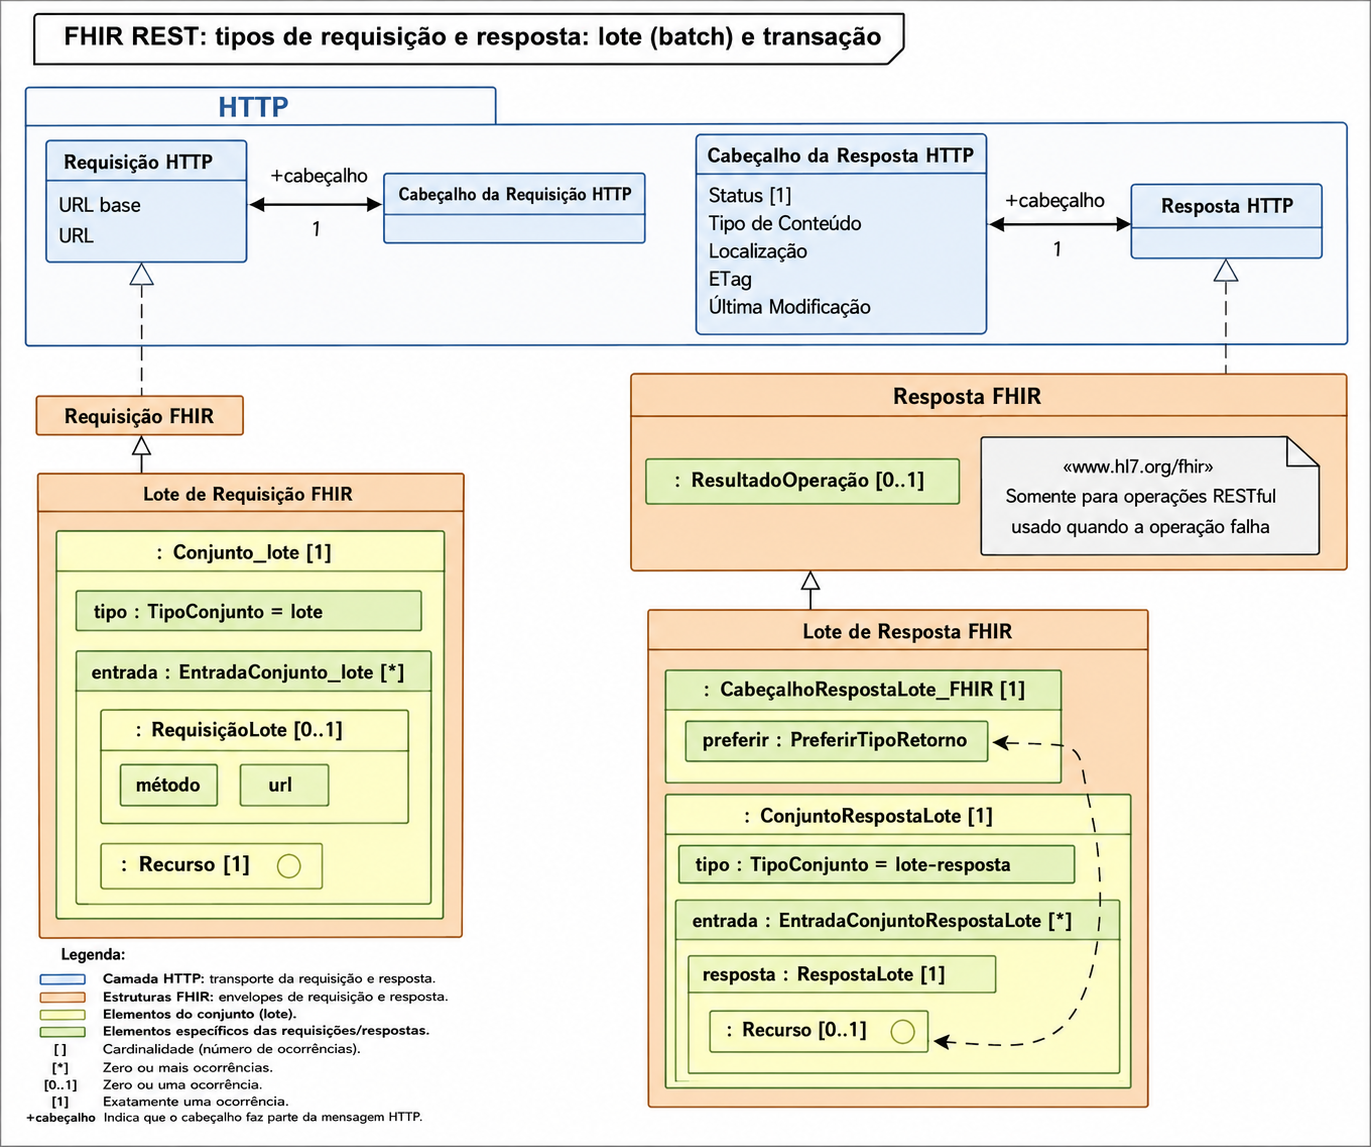
\includegraphics[width=0.85\textwidth]{FHIR.png}
%    \label{fig:fhir}
%
%    \vspace{0.2cm}
%    \footnotesize{Fonte: Adaptado de Ayaz et.al (2021)}
%\end{figure}

\begin{figure}[H]
\centering
\caption{Funcionamento FHIR}
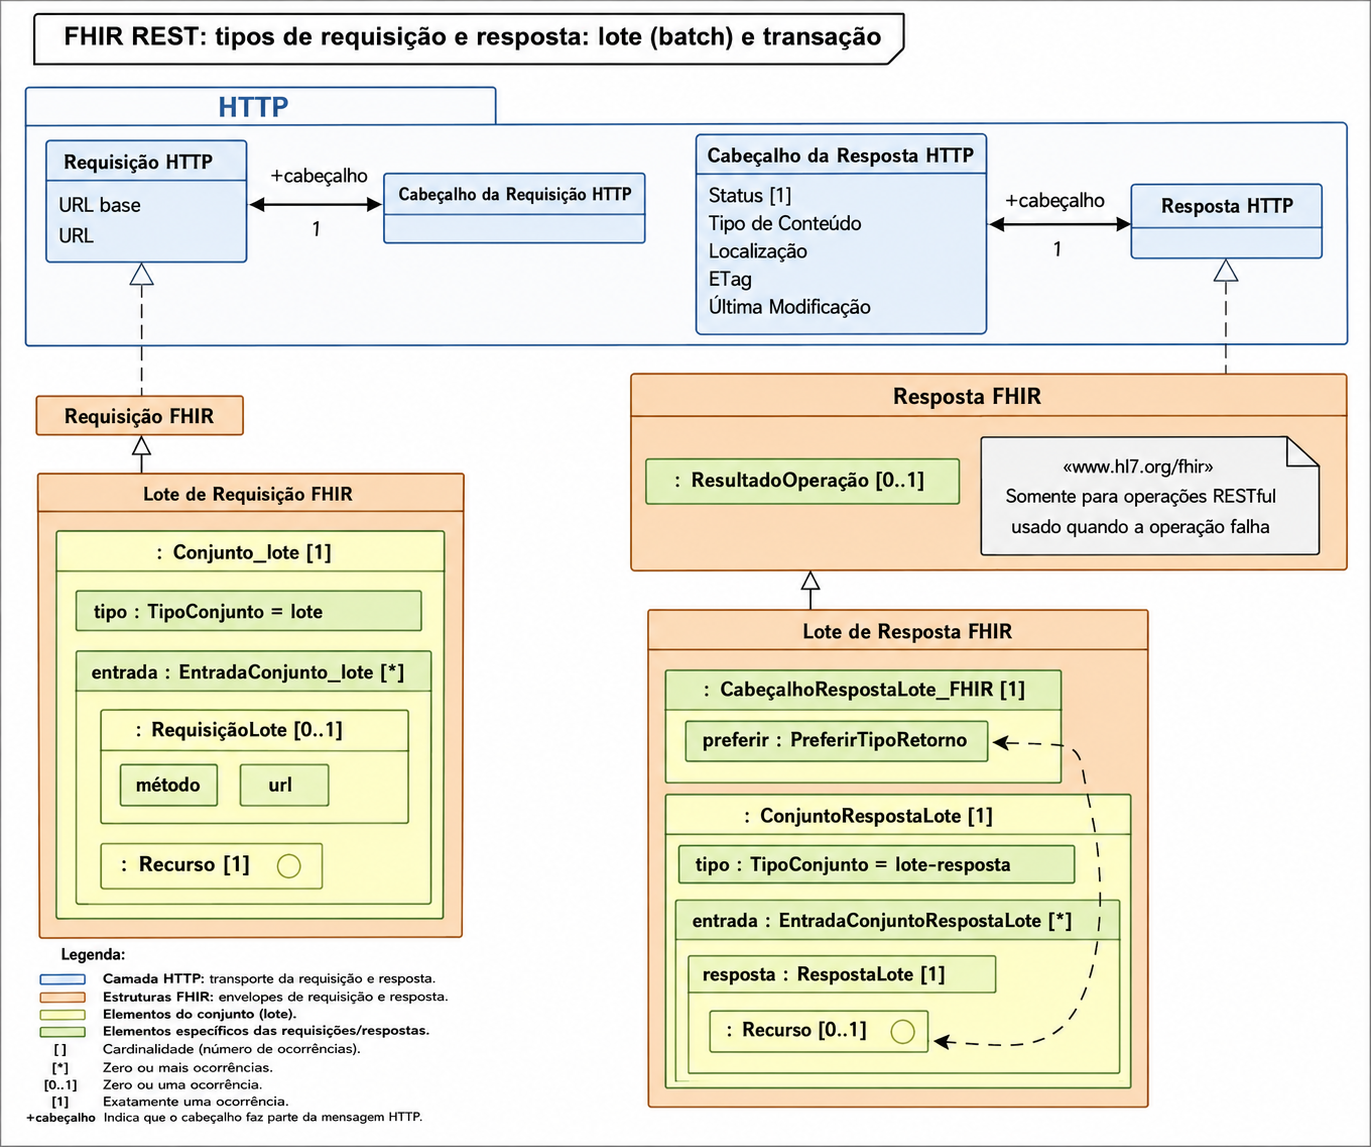
\includegraphics[width=0.85\textwidth]{FHIR.png}
\label{fig:fhir}
\vspace{0.2cm}
\footnotesize{Fonte: Adaptado de Ayaz et.al (2021)}
\end{figure}

A relevância desse padrão no contexto da saúde digital foi confirmada por revisão sistemática conduzida por Ayaz et al. (2021), que analisou 80 estudos e identificou que as principais aplicações do FHIR envolvem justamente o gerenciamento de registros eletrônicos e a integração entre sistemas hospitalares diferentes. Um exemplo prático pode ser encontrado no trabalho de Chaves et al. (2021), que desenvolveram uma aplicação web baseada em FHIR para gerenciamento de agendamentos em hospitais públicos portugueses. Os autores mostram que o uso do padrão permite configurar regras de filtragem por médico, localização e tipo de serviço, diminuindo a necessidade de intervenção humana na marcação de consultas, o que se aproxima bastante do que se propõe neste trabalho.

Dessa forma, considerar o FHIR como camada de integração para o chatbot desenvolvido representa uma escolha tecnicamente fundamentada, que aumenta as possibilidades de compatibilidade da solução com sistemas já em uso nas clínicas.

Um desafio recorrente nos sistemas de agendamento é o fenômeno do \textit{no-show}, que significa a ausência do paciente no horário agendado sem aviso prévio. Esse problema causa ociosidade nas agendas médicas e desperdício de recursos. Brancewicz et al. (2025), em estudo clínico conduzido em uma clínica de saúde mental, registraram redução significativa na taxa de \textit{no-show}, de 18,55\% em 2019 para 7,01\% em 2023, após a implantação de um sistema automatizado de confirmação de consultas com opções de seleção do tipo de atendimento por formulário digital. Esse resultado evidencia o impacto de estratégias proativas de engajamento do paciente sustentadas por tecnologia. Além disso, problemas como atrasos e má distribuição de horários representam desafios recorrentes nos sistemas de agendamento. A utilização de tecnologias automatizadas, como chatbots, pode contribuir para a redução desses problemas, permitindo o envio de lembretes automáticos, confirmação de consultas e maior flexibilidade no reagendamento, melhorando significativamente a eficiência operacional das clínicas.

% ------------------------------------------
\subsection{Lei Geral de Proteção de Dados no Contexto da Saúde}
\label{sec:lgpd}
% ------------------------------------------

A entrada em vigor da Lei Geral de Proteção de Dados (Lei n\textordmasculine{} 13.709/2018) estabeleceu um novo marco jurídico para o tratamento de informações pessoais no Brasil, visando proteger os direitos fundamentais de liberdade e privacidade. No setor da saúde, a adequação a esta legislação é considerada de alta complexidade, uma vez que as instituições manipulam dados sensíveis de forma ininterrupta para viabilizar o cuidado ao paciente.

A LGPD classifica os dados de saúde como dados pessoais sensíveis, categoria que inclui também informações sobre origem racial ou étnica, convicção religiosa, opinião política, filiação sindical, dados genéticos, dados biométricos e vida sexual. Para essa categoria, a lei estabelece requisitos mais rígidos para o tratamento, exigindo base legal específica, como o consentimento explícito do titular ou a necessidade de tutela da saúde em procedimentos realizados por profissionais de saúde ou entidades sanitárias (BRASIL, 2018). No contexto de um chatbot clínico, nome, telefone e data de nascimento são dados pessoais; a especialidade procurada e o histórico de consultas, por se referirem à saúde do titular ou permitirem inferi-la, são tratados como dados pessoais sensíveis (art. 5º, II). Por cautela, todo o conjunto recebe o nível de proteção exigido para dados sensíveis.

\subsubsection{Classificação de Dados Sensíveis e Governança}

De acordo com a legislação vigente, dados sensíveis são aqueles que revelam informações sobre a saúde, vida sexual, genética ou biometria do indivíduo. No ambiente clínico, embora estas informações sejam cruciais para o diagnóstico, o seu processamento gera desafios de conformidade que exigem uma estrutura de governança robusta.

% TRECHO ANTIGO (revisão pré-banca: uso de marcadores onde o orientador pediu texto corrido)
%Conforme Hawryliszyn, Coelho e Barja (2021), a implementação da LGPD requer:
%\begin{itemize}
%    \item Mapeamento de Dados: Identificação de todo o fluxo da informação, desde a coleta inicial no agendamento até ao armazenamento e descarte final;
%    \item Segurança e Padrões Técnicos: Manutenção de normas rígidas para impedir acessos não autorizados ou o vazamento de prontuários;
%    \item Mitigação de Riscos: Adoção de ações preventivas e educativas para reduzir a exposição de dados sensíveis em sistemas automatizados.
%\end{itemize}

% TRECHO NOVO
Conforme Hawryliszyn, Coelho e Barja (2021), a implementação da LGPD requer três frentes de atuação complementares. A primeira é o mapeamento de dados, que consiste em identificar todo o fluxo da informação, desde a coleta inicial no agendamento até o armazenamento e o descarte final. A segunda é a manutenção de segurança e padrões técnicos rígidos, capazes de impedir acessos não autorizados ou o vazamento de prontuários. A terceira é a mitigação de riscos, por meio da adoção de ações preventivas e educativas que reduzam a exposição de dados sensíveis em sistemas automatizados. Essas três frentes orientam diretamente as decisões de arquitetura do chatbot proposto, detalhadas na seção 2.4.4.

\subsubsection{Princípios da LGPD Aplicáveis ao Chatbot Proposto}

A LGPD estabelece dez princípios para o tratamento de dados pessoais, dos quais cinco são diretamente aplicáveis ao desenvolvimento do chatbot proposto neste trabalho. O princípio da finalidade determina que os dados coletados devem ser utilizados exclusivamente para os propósitos informados ao titular no momento da coleta. No caso do chatbot, os dados do paciente não podem ser usados para fins secundários sem consentimento adicional. O princípio da necessidade (art. 6º, III), também chamado de minimização, limita o tratamento ao mínimo necessário para a realização das finalidades, com dados pertinentes, proporcionais e não excessivos; no chatbot, apenas as informações estritamente necessárias ao agendamento devem ser coletadas. O princípio da segurança exige criptografia em trânsito (TLS/SSL) e em repouso, além de controles de acesso baseados em funções; no protótipo, apenas a criptografia em trânsito foi implementada (seção~\ref{sec:persistencia}). O princípio da transparência determina que o titular deve ser informado de forma clara sobre o tratamento de seus dados, materializado no chatbot por uma política de privacidade exibida no início de cada interação. Por fim, o princípio da prestação de contas exige a manutenção de logs de todas as interações, com registro de consentimento, horário, dados coletados e finalidade, de modo a permitir a auditoria dos fluxos de tratamento (HAWRYLISZYN; COELHO; BARJA, 2021).

\subsubsection{Impacto nos Sistemas de Automação e Chatbots}

A transição para sistemas automatizados de agendamento não é apenas uma mudança tecnológica, mas uma mudança cultural que exige o cumprimento de boas práticas estruturadas. Chatbots que lidam com cadastro de pacientes devem ser projetados sob o princípio da privacidade por design (\textit{privacy by design}): a proteção de dados deve ser incorporada ao sistema desde sua concepção, e não como uma camada adicionada posteriormente (CAVOUKIAN, 2009; BRASIL, 2018, art. 46, § 2º).

% TRECHO ANTIGO (revisão pré-banca: uso de marcadores onde o orientador pediu texto corrido)
%Na prática, a conformidade com a LGPD implica um conjunto de requisitos técnicos específicos:
%\begin{itemize}
%    \item O registro do consentimento explícito do paciente antes da coleta de qualquer dado, com possibilidade de revogação a qualquer momento;
%    \item A minimização da coleta, restringindo-se às informações estritamente necessárias para o agendamento;
%    \item A criptografia ponta a ponta nas comunicações entre o paciente e o sistema;
%    \item A definição de prazos de retenção de dados, com descarte seguro ao término do prazo estabelecido;
%    \item A criação de mecanismos para que o titular possa exercer seus direitos previstos na lei, como acesso, correção e exclusão de seus dados.
%\end{itemize}

% TRECHO NOVO
Na prática, a conformidade com a LGPD implica um conjunto de requisitos técnicos específicos. O primeiro é o registro do consentimento explícito do paciente antes da coleta de qualquer dado, com possibilidade de revogação a qualquer momento. O segundo é a necessidade (minimização) da coleta, restringindo-se às informações estritamente necessárias para o agendamento. O terceiro, já detalhado na seção~\ref{sec:persistencia}, é a criptografia em trânsito (TLS/SSL) nas comunicações e em repouso no armazenamento; no protótipo, apenas a primeira foi implementada. Some-se a isso a definição de prazos de retenção de dados, com descarte seguro ao término do prazo estabelecido, e a criação de mecanismos para que o titular possa exercer seus direitos previstos na lei, como acesso, correção e exclusão de seus dados.

Adotou-se o consentimento (art. 11, I) como base legal por ser o tratamento realizado por um canal de automação, sem intervenção direta de profissional de saúde, e por conferir ao titular controle por finalidade; em operação real, a clínica poderá avaliar também a hipótese de tutela da saúde (art. 11, II, ``f''). As mensagens trafegam pela infraestrutura do Telegram, que pode estar fora do Brasil, o que configura transferência internacional de dados (arts. 33 a 36) e exige, em uso real, análise das hipóteses legais. O armazenamento de eventos de conversa do Rasa e os registros do servidor e do túnel podem conter o texto integral das mensagens; no protótipo, o Rasa mantém os eventos de conversa apenas em memória, pois nenhum armazenamento persistente foi configurado, e eles são descartados quando o servidor é reiniciado; em uso real, esses registros devem seguir o prazo de 12 meses definido no requisito RNF09 e ser eliminados ao fim dele.

 A conformidade legal não apenas protege os pacientes e a clínica de riscos jurídicos e reputacionais, mas é também um fator de confiança que influencia diretamente a taxa de adoção da solução pelos usuários.

 \subsection{Trabalhos Correlatos}
\label{sec:correlatos}

Esta seção posiciona o trabalho em relação a soluções e estudos que tratam de agendamento automatizado em saúde, de modo a evidenciar a lacuna apontada na Introdução: soluções que combinem agendamento, compreensão de linguagem natural em português e conformidade com a LGPD. A Tabela~\ref{tab:correlatos} compara os trabalhos selecionados com a solução proposta, e os parágrafos seguintes apontam o que cada um resolve e o que não cobre.

Em revisão sistemática sobre agentes conversacionais com entrada em linguagem natural aplicados à saúde, Laranjo et al. (2018) incluíram 17 artigos, referentes a 14 agentes, e observaram que as estratégias de gerenciamento de diálogo eram predominantemente de estados finitos ou baseadas em formulários (\textit{frame-based}), que a maioria dos estudos tinha delineamento quase-experimental e que a segurança do paciente raramente era avaliada. A abordagem deste trabalho, com diálogo conduzido por regras e formulários e com confirmação explícita antes de registrar qualquer agendamento, alinha-se à estratégia predominante identificada na revisão e responde à preocupação com a segurança. Em revisão sistemática posterior, Milne-Ives et al. (2020) avaliaram a eficácia e a usabilidade de agentes conversacionais com processamento de linguagem natural em saúde e reuniram o que os usuários apreciam e rejeitam nesses sistemas, de modo a orientar o desenvolvimento de novos agentes.

Chaves et al. (2021) apresentaram o AIDA OGT, aplicação web baseada no padrão HL7 FHIR (recursos \textit{Schedule}, \textit{Slot} e \textit{Appointment}), desenvolvida para hospitais públicos portugueses, que oferece aos administradores hospitalares sugestões de datas para agendamento a partir de regras predefinidas. O trabalho resolve a integração interoperável com a agenda, mas é voltado à equipe do hospital, sem interação em linguagem natural com o paciente; a segurança é tratada de forma genérica, sem registro do consentimento do titular, e a validação descrita limita-se a testes unitários, sem avaliação com usuários, por se tratar de uma versão inicial.

AlSerkal et al. (2025) avaliaram, em centros de atenção primária dos Emirados Árabes Unidos, um modelo de inteligência artificial integrado ao prontuário eletrônico que prevê faltas com 86\% de acurácia e alimenta um painel usado pelos coordenadores. Na comparação antes e depois, com 135.393 agendamentos, a taxa de faltas caiu 50,7\%. A solução, porém, apoia a equipe da clínica e não o paciente, e pressupõe a infraestrutura de uma grande rede de saúde.

Brancewicz et al. (2025) implantaram, em uma clínica de saúde mental na Polônia, um sistema automatizado de confirmação de consultas por SMS, com apoio telefônico, e observaram a redução das faltas de 18,55\% para 7,01\%, com avaliação positiva de mais de 93\% dos pacientes. O sistema trata apenas da confirmação de consultas já marcadas, por respostas estruturadas e sem linguagem natural, e não permite agendar, cancelar ou reagendar.

Li et al. (2021) avaliaram, em um estudo de coorte retrospectivo com 12.342 atendimentos ambulatoriais na China, um módulo de inteligência artificial que solicita exames a partir da queixa principal do paciente, reduzindo a espera mediana de 1,97 para 0,38 hora. O trabalho mostra o ganho de eficiência da inteligência artificial no fluxo de atendimento, mas não trata do agendamento de consultas nem de interação conversacional.

Elhag, Althagafi e Almouabdi (2026) propuseram um sistema inteligente de agendamento hospitalar em que o paciente descreve os sintomas por \textit{chat}; um modelo BioBERT-BiLSTM faz a triagem (F1-score de 0,87), indica o especialista e reserva o horário automaticamente. Em simulações de processos, o tempo de marcação caiu 96,3\%, de 155 para 5,73 minutos. É o trabalho mais próximo deste, por agendar a partir de linguagem natural, mas foi avaliado apenas por simulação, sem usuários, não é em português e trata as normas de proteção de dados apenas como ameaça na análise do projeto, sem implementar o registro do consentimento.

Massa et al. (2023) desenvolveram, no Brasil, a Amanda Selfie, chatbot em português no Facebook Messenger, com o Dialogflow como motor de linguagem natural, para criar demanda pela profilaxia pré-exposição ao HIV entre adolescentes. A chatbot foi bem aceita e alcançou 757 das 1.239 pessoas atingidas pelas estratégias em redes sociais, e o diálogo complementar com um profissional de saúde facilitou o agendamento das consultas, mas a conversão em uso da profilaxia foi menor que a das demais estratégias. O agendamento dependia do profissional, o processamento ocorria em serviço de nuvem, e o consentimento registrado era o da pesquisa, e não um fluxo do próprio chatbot.

Barreto et al. (2021) apresentaram o GISSA Mamãe-Bebê, aplicativo brasileiro de conversa para a promoção da saúde infantil, com fluxos definidos por regras de decisão e processamento básico de linguagem natural (biblioteca NLTK), capaz de interpretar respostas curtas como ``s'' e ``n''. Avaliado por 142 puérperas, obteve concordância acima de 90\% quanto à clareza, à utilidade e à satisfação. O trabalho mostra a aceitação de chatbots de saúde em português, mas não realiza agendamento nem emprega um modelo de linguagem para interpretar o texto livre.

Leito et al. (2025) usaram o Rasa, com o módulo CALM, que integra modelos de linguagem de larga escala, para aplicar a idosos o questionário de estado de saúde EQ-5D, com ações customizadas e limiares de confiança para decidir quando repetir uma pergunta, recursos semelhantes aos deste protótipo. Os autores observam que há pouca pesquisa que empregue explicitamente o Rasa, o que reforça a contribuição deste trabalho; a aplicação, porém, não envolve agendamento e não é em português.

Nenhum dos trabalhos analisados combina interação em linguagem natural em português, integração com a agenda e registro do consentimento conforme a LGPD, o que caracteriza a lacuna que este trabalho busca endereçar. O mais próximo, de Elhag, Althagafi e Almouabdi (2026), agenda a partir de linguagem natural, mas foi avaliado apenas por simulação e não trata do consentimento; os dois trabalhos brasileiros, em português, não agendam de forma autônoma ou dependem de serviço de nuvem; e o que usa o Rasa não trata de agendamento.

\begin{table}[H]
\centering
\scriptsize
\caption{Comparação entre os trabalhos correlatos e a solução proposta}
\label{tab:correlatos}
\begin{tabularx}{\textwidth}{L{2.4cm}L{2.5cm}L{2.8cm}L{2.8cm}Y}
\hline
\textbf{Trabalho} & \textbf{Canal} & \textbf{NLU / técnica} & \textbf{Integração com a agenda} & \textbf{Privacidade / LGPD e avaliação} \\
\hline
Chaves et al. (2021) & Aplicação web para administradores hospitalares & Não usa linguagem natural; sugestão de datas por regras & FHIR (\textit{Schedule}, \textit{Slot}, \textit{Appointment}), com filtros por médico, local e tipo de serviço & Segurança tratada de forma genérica; sem consentimento; testes unitários, sem avaliação com usuários \\
AlSerkal et al. (2025) & Painel para coordenadores, sem interação com o paciente & Modelo preditivo de faltas (acurácia de 86\%) & Integrado ao prontuário eletrônico & Não trata da LGPD (Emirados Árabes); antes e depois com 135.393 agendamentos: faltas $-$50,7\% \\
Brancewicz et al. (2025) & SMS e telefone & Sem linguagem natural: confirmação automática com resposta rápida & Sistema automatizado de confirmação de consultas & Não trata da LGPD (Polônia); faltas de 18,55\% para 7,01\%; 93\% acharam o sistema intuitivo \\
Li et al. (2021) & Módulo no fluxo ambulatorial (XIAO YI) & Inteligência artificial que solicita exames a partir da queixa principal & Integrado ao fluxo do hospital, antes da consulta & Não trata da LGPD (China); 12.342 atendimentos: espera mediana de 1,97 h para 0,38 h \\
Elhag, Althagafi e Almouabdi (2026) & \textit{Chat} de sintomas no sistema hospitalar & BioBERT-BiLSTM para triagem (F1 0,87) & Agendamento automático com o especialista indicado & Normas de dados só citadas como ameaça; avaliação por simulação: tempo de marcação $-$96,3\% \\
Massa et al. (2023) & Facebook Messenger, em português & Dialogflow (serviço de nuvem) & Encaminha para agendamento feito com apoio de profissional & Consentimento da pesquisa; 757 de 1.239 alcançados; boa aceitação \\
Barreto et al. (2021) & Aplicativo móvel, em português & Fluxos por regras de decisão; PLN básico (NLTK) & Não realiza agendamento & Consentimento da pesquisa (TCLE); 142 puérperas, concordância acima de 90\% \\
Leito et al. (2025) & Chatbot de questionário de saúde & Rasa com CALM (integra LLM); limiares de confiança & Não realiza agendamento & Não trata de proteção de dados; protótipo demonstrativo \\
\textbf{Solução proposta} & Telegram & DIET com BERTimbau (Rasa) & Banco local modelado a partir do FHIR (simulado) & Consentimento por finalidade; núcleo local; F1, acurácia, tempo de resposta e SUS \\
\hline
\end{tabularx}
\vspace{0.3cm}

\footnotesize{Fonte: Elaborado pelo autor (2026).}
\end{table}

% ==========================================
% METODOLOGIA
% ==========================================
\newpage
\section{Metodologia}
\label{cap:metodologia}

Este capítulo descreve os procedimentos metodológicos adotados para a análise, modelagem, desenvolvimento e avaliação do chatbot baseado em Inteligência Artificial para automação de processos administrativos e otimização do agendamento de consultas em clínicas médicas. A metodologia foi definida a partir do problema identificado, relacionado à sobrecarga operacional das equipes de recepção, à lentidão no atendimento ao paciente e à necessidade de soluções acessíveis para clínicas médicas de pequeno e médio porte. Os procedimentos descritos orientam a construção e a avaliação do artefato tecnológico proposto (GIL, 2002).

\subsection{Tipo de Pesquisa}

A presente pesquisa caracteriza-se quanto à sua natureza como aplicada, quanto aos seus objetivos como exploratório-descritiva e quanto à abordagem como quali-quantitativa: a dimensão qualitativa orienta a análise de requisitos, fluxos e implicações legais, e a quantitativa, a avaliação do protótipo. Além disso, são empregados procedimentos técnicos relacionados à pesquisa bibliográfica e documental, bem como ao desenvolvimento e à avaliação experimental do artefato tecnológico.

\subsubsection{Natureza da pesquisa}

Quanto à sua natureza, esta pesquisa é classificada como aplicada, uma vez que busca gerar conhecimento direcionado à solução de um problema prático específico: a ineficiência de determinados processos administrativos em clínicas médicas e a necessidade de ferramentas adequadas às características de clínicas de pequeno e médio porte (PRODANOV; FREITAS, 2013).

A pesquisa aplicada mostra-se adequada ao presente trabalho porque seus resultados não se limitam à discussão teórica sobre Inteligência Artificial, Processamento de Linguagem Natural ou automação de processos. O estudo também contempla a construção de um artefato tecnológico destinado a atender a uma necessidade identificada no contexto de clínicas médicas, permitindo avaliar sua utilização em processos administrativos relacionados ao atendimento e ao agendamento de consultas.

\subsubsection{Abordagem metodológica}

Quanto à abordagem, a pesquisa é quali-quantitativa (métodos mistos), com análise de requisitos, fluxos e implicações legais combinada à avaliação quantitativa do protótipo. A abordagem qualitativa permite analisar os requisitos funcionais do sistema, os fluxos de atendimento das clínicas médicas, as características das interações entre usuários e chatbot e as implicações relacionadas ao tratamento de dados pessoais no contexto da saúde (CRESWELL; CRESWELL, 2021).

A dimensão quantitativa é utilizada principalmente na avaliação do desempenho do protótipo. Para isso, são consideradas métricas como precisão, revocação e F1-score, aplicadas à avaliação do módulo de compreensão de linguagem natural, além da pontuação obtida por meio do instrumento \textit{System Usability Scale} (SUS), utilizado para avaliação da usabilidade do sistema (BROOKE, 1996).

Dessa forma, a combinação das duas abordagens permite analisar tanto aspectos qualitativos relacionados ao funcionamento e à adequação do sistema quanto resultados quantitativos obtidos durante sua avaliação.

\subsubsection{Procedimentos técnicos}

Quanto aos procedimentos técnicos, a pesquisa combina levantamento bibliográfico e documental com o desenvolvimento de um protótipo tecnológico. O levantamento bibliográfico é utilizado para fundamentar os conceitos relacionados a chatbots, Inteligência Artificial, Processamento de Linguagem Natural, classificação de intenções, reconhecimento de entidades, modelos Transformer, BERTimbau, automação de processos e sistemas de agendamento em clínicas médicas.

A pesquisa documental contempla a análise de legislação, documentação técnica e especificações relacionadas ao domínio da aplicação, incluindo a Lei Geral de Proteção de Dados (LGPD), documentação relacionada ao framework Rasa, ao modelo BERTimbau e ao padrão HL7 FHIR.

O desenvolvimento do sistema constitui a etapa experimental da pesquisa, na qual os conhecimentos obtidos nas etapas anteriores são utilizados para construção e avaliação do artefato tecnológico.

\subsection{Procedimentos Metodológicos}
\label{sec:procedimentos}

A pesquisa foi conduzida por meio da combinação entre levantamento bibliográfico, pesquisa documental e desenvolvimento iterativo do protótipo. Como método central, adotou-se a \textit{Design Science Research} (DSR), abordagem utilizada em pesquisas de Sistemas de Informação para orientar a concepção, construção e avaliação de artefatos tecnológicos destinados à solução de problemas práticos.

Conforme Hevner et al. (2004), a DSR estabelece que o artefato desenvolvido deve apresentar relevância para o contexto de aplicação, fundamentação adequada em conhecimentos existentes e contribuição para o domínio no qual está inserido. Nesse sentido, o chatbot proposto é direcionado ao contexto de clínicas médicas de pequeno e médio porte, fundamentando-se na literatura científica e técnica apresentada no referencial teórico e buscando oferecer uma solução de execução local para automação de processos administrativos.

A Tabela~\ref{tab:dsr} relaciona as atividades da \textit{Design Science Research}, segundo o modelo de Peffers et al. (2007), às partes deste trabalho em que cada uma é realizada.

\begin{table}[H]
\centering
\caption{Mapeamento das atividades da \textit{Design Science Research} neste trabalho}
\label{tab:dsr}
\small
\begin{tabularx}{\textwidth}{p{5.2cm}Y}
\hline
\textbf{Atividade (PEFFERS et al., 2007)} & \textbf{Onde é realizada neste trabalho} \\
\hline
1. Identificação do problema e motivação & Seção~\ref{cap:intro} (problema e justificativa). \\
2. Definição dos objetivos da solução & Objetivos da Seção~\ref{cap:intro} e Tabela~\ref{tab:criterios-sucesso} (critérios mensuráveis). \\
3. Projeto e desenvolvimento & Seções~\ref{cap:metodologia} (desenvolvimento iterativo) e~\ref{cap:projeto} (requisitos, modelagem e banco de dados). \\
4. Demonstração & Seção~\ref{cap:resultados}: execução dos cenários simulados no Telegram. \\
5. Avaliação & Seção~\ref{cap:resultados}: métricas de NLU, taxa de aprovação nos cenários de teste, tempo de resposta e SUS; avaliação artificial e \textit{ex post} (VENABLE; PRIES-HEJE; BASKERVILLE, 2016). \\
6. Comunicação & Este trabalho. \\
\hline
\end{tabularx}
\vspace{0.3cm}

\footnotesize{Fonte: Elaborado pelo autor (2026), com base em Peffers et al. (2007) e Venable, Pries-Heje e Baskerville (2016).}
\end{table}

O cenário de aplicação considerado corresponde às clínicas médicas de pequeno e médio porte localizadas na região de Foz do Iguaçu e entorno. O público-alvo do sistema é composto por estabelecimentos desse segmento, caracterizados, no contexto delimitado pela pesquisa, pela possibilidade de apresentarem equipes de recepção reduzidas e elevada demanda de atendimento.

Os processos administrativos considerados no desenvolvimento são o agendamento de consultas, o cancelamento, o reagendamento, o envio de lembretes automáticos e o fornecimento de informações sobre convênios aceitos. Esses processos foram selecionados por apresentarem fluxos suficientemente estruturados para permitir sua automação por meio de um chatbot baseado em Processamento de Linguagem Natural.

Embora o público-alvo do sistema seja constituído por clínicas médicas de pequeno e médio porte, a validação do protótipo foi realizada em ambiente simulado, uma vez que não havia, nesta etapa da pesquisa, uma clínica parceira formalmente vinculada ao projeto. Dessa forma, não foram utilizados dados reais de pacientes. A agenda médica utilizada pelo protótipo foi simulada por meio de um banco de dados local, estruturado com base nos recursos \textit{Schedule}, \textit{Slot} e \textit{Appointment} do padrão HL7 FHIR.

\subsubsection{Métodos de coleta de informações}
\label{sec:coleta}

A coleta das informações necessárias ao desenvolvimento da pesquisa foi realizada por meio de pesquisa bibliográfica, pesquisa documental e levantamento dos requisitos necessários à construção do protótipo.

A pesquisa bibliográfica foi realizada nas bases IEEE Xplore, ACM Digital Library, Google Scholar, SciELO e PubMed/NCBI, utilizando descritores em português e inglês relacionados aos temas abordados neste trabalho, tais como ``chatbot'', ``chatbot saúde'', ``NLP healthcare'', ``intent classification'', ``named entity recognition medical'', ``automação agendamento clínica'', ``LGPD saúde'', ``no-show reduction'', ``BERTimbau'' e ``Rasa NLU''.

Os critérios de inclusão priorizaram publicações de 2015 a 2025, com ênfase em artigos revisados por pares e estudos empíricos, admitindo-se exceção para obras seminais e de referência consolidada (por exemplo, Weizenbaum, 1966; Searle, 1980; Brooke, 1996; Hevner et al., 2004; Mikolov et al., 2013) e para documentação técnica e legislação, independentemente do ano. A pesquisa bibliográfica teve caráter narrativo, sem protocolo sistemático de revisão. A seleção das fontes buscou reunir informações relacionadas aos fundamentos teóricos e técnicos necessários para a construção do chatbot.

A pesquisa documental contemplou a legislação pertinente, incluindo a Lei nº 13.709/2018 (LGPD), documentos e diretrizes relacionados ao tratamento de dados pessoais e documentação técnica referente às tecnologias e padrões empregados no desenvolvimento. Também foram consideradas especificações relacionadas ao framework Rasa, ao modelo BERTimbau e ao padrão HL7 FHIR.

Além da pesquisa bibliográfica e documental, foram levantados os requisitos funcionais do protótipo a partir dos processos administrativos definidos para o cenário de aplicação. Esses requisitos orientaram a definição das intenções, entidades e cenários de interação utilizados no desenvolvimento e na avaliação do chatbot.

\subsubsection{Métodos de análise das informações}

As informações obtidas na pesquisa bibliográfica foram organizadas por meio de síntese narrativa, agrupada pelos temas chatbots, Processamento de Linguagem Natural, automação de processos administrativos, sistemas de agendamento, interoperabilidade em saúde e privacidade de dados, sem aplicação de técnica formal de análise de conteúdo, em coerência com o caráter narrativo da revisão.

A análise documental possui caráter normativo-comparativo, buscando verificar a relação entre os requisitos identificados nos documentos analisados e as decisões adotadas no desenvolvimento do sistema. No contexto da LGPD, foram considerados especialmente os princípios relacionados à finalidade, necessidade, segurança, transparência e prestação de contas.

As informações obtidas durante o levantamento dos requisitos foram utilizadas para definir os fluxos de interação do chatbot, as intenções que ele deveria reconhecer, as entidades necessárias para a execução das tarefas e os cenários utilizados posteriormente nos testes.

Os resultados obtidos durante a avaliação do protótipo foram analisados de maneira integrada. As métricas quantitativas de desempenho foram utilizadas em conjunto com a análise qualitativa dos erros de classificação e das situações nas quais o sistema não consegue atender adequadamente à solicitação do usuário. Essa análise orientou os ciclos de refinamento do protótipo até a obtenção da versão final do sistema.

\subsection{Metodologia de Desenvolvimento do Sistema}

O desenvolvimento do sistema foi realizado de maneira iterativa, seguindo as etapas definidas pela abordagem de \textit{Design Science Research}. Inicialmente foram identificados os processos administrativos a serem automatizados e definidos os requisitos do chatbot. Em seguida, foram construídos os fluxos de conversação, o corpus de treinamento e os componentes responsáveis pela compreensão das mensagens dos usuários.

Após a implementação dos componentes principais, o sistema foi submetido aos cenários de teste definidos para a pesquisa. Os resultados obtidos foram utilizados para identificar falhas, ajustar o comportamento do sistema e realizar novos ciclos de avaliação.

O núcleo do protótipo foi executado localmente, sem envio de dados dos usuários a serviços de processamento externos (o canal de mensageria é a exceção, declarada na seção~\ref{sec:limitacoes}), mantendo a proposta de utilização de uma arquitetura adequada ao contexto de tratamento de dados sensíveis de saúde.

\subsubsection{Modelo de desenvolvimento de software}

O desenvolvimento do protótipo seguiu uma abordagem iterativa, na qual o sistema foi construído e aperfeiçoado progressivamente a partir dos resultados obtidos durante as etapas de desenvolvimento e avaliação.

Essa abordagem é adequada ao projeto porque permite que os componentes do chatbot sejam implementados gradualmente. Inicialmente foram definidos os fluxos de atendimento e as intenções do sistema. Posteriormente, foram desenvolvidos e treinados os componentes de compreensão de linguagem natural, integrados aos fluxos de atendimento e submetidos aos cenários de teste.

Os resultados dos testes foram utilizados para identificar problemas de classificação, extração de entidades e execução dos fluxos. Quando necessário, o corpus e os componentes do sistema foram refinados, o que permitiu a realização de novos ciclos de treinamento e avaliação.

\subsubsection{Tecnologias utilizadas}

O protótipo utiliza tecnologias selecionadas de acordo com os requisitos identificados no contexto da pesquisa.

O Rasa Open Source é utilizado como framework principal para o desenvolvimento do chatbot, permitindo a implementação dos componentes responsáveis pela compreensão das mensagens dos usuários e pelo gerenciamento dos fluxos de conversação. A escolha do Rasa está relacionada à possibilidade de execução local e ao controle sobre o processamento dos dados.

O modelo BERTimbau (\texttt{neuralmind/\allowbreak bert-base-\allowbreak portuguese-cased}) é utilizado como extrator de características do \textit{pipeline} de NLU, por meio do componente \texttt{LanguageModel\allowbreak{}Featurizer} do Rasa, cuja saída densa é combinada com características esparsas (\textit{bag-of-words} de palavras e de caracteres) e alimenta o classificador \texttt{DIETClassifier}, responsável pela classificação de intenções e pela extração de entidades (BUNK et al., 2020). A combinação de representações densas e esparsas é adequada a corpora pequenos, como o deste protótipo. A configuração completa do \textit{pipeline} está no Apêndice~\ref{ap:config}.

O banco de dados local é utilizado para representar a agenda médica simulada e armazenar as informações necessárias à execução dos fluxos definidos para o protótipo. A estrutura considera os recursos \textit{Schedule}, \textit{Slot} e \textit{Appointment}, relacionados ao padrão HL7 FHIR.

O protótipo é implementado em Python 3.8, com a versão 3.6.20 do Rasa Open Source e a versão 3.6.2 do Rasa SDK. A lógica de negócio é executada em ações customizadas (\textit{custom actions}) servidas por um servidor de ações independente do servidor de diálogo. O banco de dados local é o SQLite, acessado diretamente pelas ações. A conversa ocorre pelo Telegram, por meio da API de bots, e, durante o desenvolvimento, o servidor local é exposto ao Telegram por um túnel HTTPS (ngrok). O canal de entrada nativo do Rasa para o Telegram apresentou falha de execução no ambiente utilizado (\texttt{RuntimeError: Event loop is closed}, originada na biblioteca \texttt{aiogram}); por isso foi desenvolvido um canal customizado, que recebe as mensagens pelo \textit{webhook} e responde diretamente pela API HTTP do Telegram. O envio dos lembretes é realizado por um serviço independente, escrito em Python, que consulta periodicamente o banco de dados.

\textbf{Recursos de hardware.} O desenvolvimento, o treinamento do modelo e todos os testes foram realizados em um único notebook, com processador AMD Ryzen 5 7235HS, cerca de 12 GB de memória e sistema operacional Windows 11, sem uso de placa de vídeo dedicada nem de servidores externos, o que é coerente com a proposta de execução local em clínicas de pequeno porte. Para a interação pelo Telegram, foi usado o aplicativo em um telefone celular e na versão web.

\textbf{Recursos de software.} Além das tecnologias citadas, foram utilizados o editor Visual Studio Code, para o código e o texto; o Git, para o controle de versões; a distribuição TeX Live, para a redação do trabalho em \LaTeX; e o Google Forms, para a aplicação do questionário SUS. As ferramentas empregadas nos testes estão listadas na Tabela~\ref{tab:ferramentas}.

\textbf{Ferramentas de prototipação.} Por se tratar de uma interface conversacional, executada dentro do aplicativo de mensagens, não foram usadas ferramentas de prototipação de telas, como o Figma. Os fluxos de conversa foram projetados como diagramas de atividades (seção~\ref{sec:modelagem-uml}) e implementados diretamente nas regras e nos formulários do Rasa, o que permitiu testá-los no próprio canal desde as primeiras versões; os diagramas do trabalho foram elaborados em TikZ.

A utilização dessas tecnologias está diretamente relacionada aos requisitos de execução local, processamento em português brasileiro, automação dos processos administrativos e simulação da integração com sistemas de agendamento.

\subsubsection{Arquitetura do sistema}
\label{sec:arquitetura}

A arquitetura do protótipo é organizada de forma a separar os componentes responsáveis pela comunicação com o usuário, compreensão da linguagem, gerenciamento do fluxo conversacional e persistência dos dados.

O fluxo inicia-se com o recebimento da mensagem enviada pelo usuário. A mensagem é encaminhada ao componente de compreensão de linguagem natural, responsável pela identificação da intenção e pela extração das entidades relevantes. A partir dessas informações, o componente responsável pelo gerenciamento da conversa determina a ação que deverá ser executada.

As ações relacionadas aos processos administrativos consultam ou modificam as informações armazenadas no banco de dados local. No caso do agendamento, por exemplo, o sistema verifica a disponibilidade de horários, registra a solicitação e retorna ao usuário a confirmação correspondente.

A arquitetura também contempla uma intenção de contenção (\textit{fallback}), utilizada para tratar mensagens que estejam fora do escopo definido para o sistema. Essa estratégia reduz a possibilidade de o chatbot executar ações inadequadas quando não conseguir compreender corretamente a solicitação. No protótipo, o componente \texttt{FallbackClassifier} aciona a intenção \texttt{nlu\_\allowbreak{}fallback} quando a confiança da melhor intenção é inferior a 0,70 ou quando a diferença entre as duas melhores intenções é inferior a 0,10; no gerenciamento do diálogo, a \texttt{RulePolicy} aciona a ação \texttt{action\_\allowbreak{}encaminhar\_\allowbreak{}atendimento\_\allowbreak{}humano} quando a confiança da política é inferior a 0,40 (RF12).

O corpus de treinamento utilizado pelo módulo de compreensão de linguagem natural é construído de forma sintética pelo pesquisador, sem utilização de dados reais de pacientes. As seis intenções iniciais do projeto (\texttt{agendarConsulta}, \texttt{cancelarConsulta}, \texttt{reagendarConsulta}, \texttt{informarConvenio}, \texttt{confirmarLembrete} e \texttt{fora\_\allowbreak{}do\_\allowbreak{}escopo}) foram ampliadas durante a implementação para atender aos fluxos de conversação. O protótipo passou a contemplar, além delas, as intenções \texttt{afirmar}, \texttt{negar}, \texttt{negar\_\allowbreak{}data}, \texttt{saudacao}, \texttt{despedida}, \texttt{agradecimento}, \texttt{horario\_\allowbreak{}funcionamento}, \texttt{endereco\_\allowbreak{}clinica}, \texttt{consultar\_\allowbreak{}preco\_\allowbreak{}particular}, \texttt{consultarAgendamento}, \texttt{falar\_\allowbreak{}com\_\allowbreak{}atendente}, \texttt{emergencia}, \texttt{atualizar\_\allowbreak{}cadastro}, \texttt{revogar\_\allowbreak{}consentimento} e \texttt{politica\_\allowbreak{}privacidade}, além da intenção \texttt{nlu\_\allowbreak{}fallback}, gerada pelo classificador de contenção.

O corpus final contém 703 frases distribuídas em 21 intenções, em número variável por intenção (Tabela~\ref{tab:distribuicao-corpus}, Apêndice~\ref{ap:corpus}). As frases contemplam sinônimos, variações linguísticas, diferentes níveis de formalidade, frases com e sem entidades explícitas e erros de digitação.

As entidades consideradas no protótipo são \texttt{data}, \texttt{horário}, \texttt{especialidade} e \texttt{convênio}. Essas entidades foram anotadas manualmente pelo pesquisador por meio da marcação do trecho correspondente em cada sentença.

O corpus foi dividido em 80\% para treinamento e 20\% para teste, de forma estratificada por intenção. Também foi utilizada validação cruzada \textit{k-fold}, com $k=5$, buscando obter estimativas mais estáveis das métricas de desempenho.
\vspace{0.5em}
No protótipo, o gerenciamento do diálogo é feito por regras determinísticas (\textit{rules}) e por formulários (\textit{forms}) do Rasa, e não por histórias de treinamento; por isso, a única política de diálogo configurada é a \texttt{RulePolicy} (Apêndice~\ref{ap:config}). Essa escolha reduz a ambiguidade de decisões probabilísticas nos fluxos administrativos, nos quais um desvio de caminho poderia gerar um agendamento incorreto ou um tratamento de dados sem consentimento. Os formulários conduzem a coleta de dados passo a passo, com validação de cada resposta, e podem ser interrompidos pelo paciente a qualquer momento. A arquitetura resultante é composta por quatro processos: (i) o servidor do Rasa, responsável pela compreensão de linguagem e pelo diálogo; (ii) o servidor de ações, que acessa o banco de dados; (iii) o canal de mensageria, que conecta o Telegram ao servidor do Rasa; e (iv) o serviço de lembretes, que opera de forma assíncrona em relação à conversa.


\subsection{Procedimentos de Teste e Validação}
\label{sec:testes-metodo}

Como não são utilizados dados reais de pacientes nem participantes identificáveis, a validação funcional foi realizada por meio de cenários simulados elaborados pelo pesquisador. A avaliação de usabilidade contou com voluntários adultos que responderam anonimamente ao questionário SUS, após aceitarem um termo de consentimento (Apêndice~\ref{ap:sus}). Esses cenários representam situações de atendimento que podem ocorrer em clínicas médicas de pequeno e médio porte.

\subsubsection{Tipos de testes aplicados}
\label{sec:tipos-metodo}

Foram realizados testes funcionais para verificar se cada funcionalidade apresenta o comportamento esperado. Esses testes abrangem os fluxos de agendamento, cancelamento, reagendamento, consulta de convênios e confirmação de lembretes.

Também foram realizados testes de integração entre os componentes responsáveis pelo processamento das mensagens, gerenciamento da conversa e persistência das informações no banco de dados local.

Os testes de desempenho do módulo de Processamento de Linguagem Natural foram realizados por meio das métricas de precisão, revocação e F1-score, calculadas no conjunto de teste separado do corpus de treinamento e por validação cruzada.

A usabilidade foi avaliada por meio do instrumento \textit{System Usability Scale} (SUS), composto por dez itens e utilizado para obtenção de uma pontuação geral de usabilidade (BROOKE, 1996).

\subsubsection{Cenários de teste}
\label{sec:cenarios-metodo}

Os cenários de teste foram construídos para representar os principais fluxos administrativos definidos para o chatbot. Cada cenário possui uma situação inicial, uma solicitação do usuário e um resultado esperado.

Os principais cenários considerados são:

\begin{itemize}
    \item Agendamento de nova consulta;
    \item Cancelamento de consulta previamente agendada;
    \item Reagendamento de consulta com identificação de data e especialidade;
    \item Consulta sobre os convênios aceitos pela clínica;
    \item Envio de lembrete automático e confirmação da consulta;
    \item Entrada de mensagens fora do escopo previsto, verificando o comportamento da intenção \textit{fallback}.
    \item Cadastro de novo paciente com consentimento integral, com consentimento apenas para o agendamento (recusa dos lembretes) e com recusa do consentimento;
    \item Interrupção do cadastro pelo paciente (``cancelar'') e respostas inválidas (nome incompleto, data impossível, telefone inválido, convênio inexistente);
    \item Atualização de dados cadastrais, com preservação dos dados não alterados;
    \item Revogação do consentimento (total e apenas dos lembretes) e posterior concessão de novo consentimento;
    \item Solicitação da política de privacidade;
    \item Pedido de agendamento sem especialidade informada, verificando se o chatbot solicita a especialidade antes de oferecer horários;
    \item Envio do lembrete, confirmação de presença e reenvio quando não há confirmação.
\end{itemize}

No cenário de agendamento, por exemplo, o usuário informa uma solicitação compatível com a intenção \texttt{agendarConsulta}. O sistema deve interpretar a solicitação, identificar as informações necessárias, consultar a agenda simulada e retornar uma resposta correspondente à disponibilidade encontrada.

No cenário de cadastro, o usuário solicita um agendamento sem possuir cadastro. O sistema deve apresentar o texto de consentimento antes de solicitar qualquer dado pessoal, registrar o consentimento somente após o aceite explícito, validar cada dado informado e, ao final, retomar o agendamento interrompido. No cenário de recusa, nenhum dado pessoal deve ser gravado. No cenário de revogação, o sistema deve registrar a data da revogação, cancelar os lembretes pendentes e exigir novo consentimento para novos agendamentos.

No cenário de reagendamento, o sistema deve reconhecer a intenção \newline \texttt{reagendarConsulta} e identificar as entidades necessárias, como data e especialidade. Nos casos em que a informação necessária não estiver disponível, o chatbot deve solicitar os dados complementares antes de executar a ação.

Os cenários de cancelamento, consulta de convênio e confirmação de lembrete seguem a mesma lógica, considerando a intenção correspondente e o resultado esperado para cada fluxo.

\subsubsection{Métricas coletadas}
\label{sec:metricas-metodo}

A avaliação do desempenho do módulo de compreensão de linguagem natural utiliza as métricas de precisão (\textit{precision}), revocação (\textit{recall}) e F1-score.

A precisão representa a proporção de classificações positivas realizadas corretamente pelo sistema em relação ao total de classificações positivas realizadas. A revocação representa a capacidade do sistema de identificar corretamente as ocorrências pertencentes a determinada classe. O F1-score representa a média harmônica entre precisão e revocação, permitindo uma avaliação conjunta dessas duas dimensões.

As métricas são calculadas por intenção e por entidade, utilizando o conjunto de teste separado do corpus de treinamento.
Além das métricas relacionadas ao desempenho do modelo, a avaliação considera a pontuação obtida pelo instrumento SUS. O questionário é composto por dez itens e fornece uma pontuação geral de usabilidade, permitindo avaliar a percepção de facilidade de utilização do protótipo (BROOKE, 1996).

Também foi considerada a taxa de aprovação nos cenários de teste, correspondente à proporção de execuções dos cenários simulados em que o chatbot concluiu corretamente a tarefa solicitada. Como os cenários foram escritos e executados pelo próprio pesquisador, essa taxa funciona como teste de regressão dos fluxos e não equivale à taxa de conclusão de tarefas por usuários reais.

\subsubsection{Critérios de aceitação}
\label{sec:criterios-metodo}

Os critérios de aceitação estabelecem as condições mínimas para considerar o protótipo adequado aos objetivos definidos na pesquisa.

Para o desempenho do módulo de compreensão de linguagem natural, estabelece-se como objetivo um F1-score mínimo de 0,80. Esse valor foi utilizado como referência para verificar se o classificador apresenta desempenho suficiente para reconhecer as principais intenções previstas no sistema.

Para a avaliação da usabilidade, estabelece-se como referência uma pontuação mínima de 68 pontos no instrumento SUS, valor utilizado como referência para a interpretação da usabilidade do sistema.

Para os fluxos administrativos, estabeleceu-se como objetivo uma taxa mínima de aprovação de 85\% nos cenários de teste, ou seja, ao menos 85\% das execuções dos cenários deveriam ser concluídas corretamente pelo chatbot.

Além dos critérios quantitativos, o protótipo deveria atender aos seguintes requisitos funcionais:

\begin{itemize}
    \item reconhecer as principais intenções definidas para o sistema;
    \item identificar as entidades necessárias para a execução dos fluxos;
    \item realizar corretamente os processos de agendamento, cancelamento e reagendamento simulados;
    \item fornecer informações sobre convênios de acordo com os dados disponíveis;
    \item realizar o fluxo de confirmação de lembretes;
    \item direcionar mensagens fora do escopo para o mecanismo de contenção (\textit{fallback});
    \item utilizar a agenda simulada armazenada no banco de dados local;
    \item executar o processamento do protótipo localmente, sem utilização de dados reais de pacientes.
\end{itemize}

O atendimento conjunto desses critérios foi utilizado como base para determinar se o artefato desenvolvido atingiu os objetivos estabelecidos para a pesquisa.


\subsubsection{Aspectos éticos}
\label{sec:aspectos-eticos}

A avaliação de usabilidade foi realizada por meio de questionário anônimo, aplicado a cinco participantes voluntários maiores de 18 anos, por formulário on-line. Não foram coletados nome, e-mail, documento ou qualquer outro dado que permitisse identificar os respondentes, e as respostas foram analisadas somente de forma agregada. Antes de iniciar, cada participante foi informado sobre o objetivo da avaliação, o caráter voluntário e anônimo da participação e a possibilidade de desistir a qualquer momento, e só prosseguiu após manifestar seu consentimento (Apêndice~\ref{ap:sus}). Durante as tarefas com o chatbot, os participantes utilizaram apenas dados fictícios; o identificador da conta do Telegram, recebido automaticamente pelo sistema, ficou restrito a um banco de dados de teste, não foi associado às respostas do questionário e foi eliminado ao final da avaliação. A coleta de dados com os participantes restringiu-se ao questionário SUS; os registros de funcionamento do protótipo no banco de dados de teste foram usados apenas na depuração técnica do sistema, e não como dados de pesquisa.

As perguntas trataram exclusivamente da percepção dos participantes sobre a usabilidade do sistema, sem abordar temas sensíveis. Por se tratar de pesquisa de opinião com participantes não identificados, o estudo enquadra-se na hipótese de dispensa de registro e avaliação pelo sistema CEP/Conep prevista no art. 1º, parágrafo único, inciso I, da Resolução CNS nº 510/2016 (BRASIL, 2016), razão pela qual não foi submetido a Comitê de Ética em Pesquisa.


\subsection{Declaração de Uso de Inteligência Artificial}

Neste trabalho foi utilizada uma única ferramenta de inteligência artificial generativa, o Claude (Anthropic), por meio do assistente conversacional claude.ai e da ferramenta Claude Code, ao longo de 2026. Ela apoiou o autor na revisão e na edição do texto, na busca e na conferência de referências, no desenvolvimento e na correção de partes do código do protótipo e dos \textit{scripts} de teste, nos cálculos da análise dos resultados e na elaboração de figuras.

Todo código e todo número apresentados foram executados ou recalculados pelo autor, e as referências foram conferidas nas fontes. Durante o uso, a ferramenta também propôs soluções inadequadas, que foram identificadas nos testes ou na revisão e corrigidas antes de chegar à versão final.

As decisões de pesquisa, incluindo a formulação do problema, os objetivos, as escolhas metodológicas, a interpretação dos resultados e as conclusões, são do autor, que responde por todo o conteúdo deste trabalho.

\begin{table}[H]
\centering
\caption{Síntese do Delineamento Metodológico}
\label{tab:delineamento}
% TABELA REFORMATADA EM PADRÃO ABNT (sem bordas verticais) E SINCRONIZADA COM A
% REDAÇÃO ATUAL DOS OBJETIVOS ESPECÍFICOS (seção 1.3.2)
\begin{tabular}{p{5.0cm}p{2.9cm}p{3.4cm}p{3.4cm}}
\hline
\textbf{Objetivo Específico} & \textbf{Instrumentos de Coleta} & \textbf{Técnica de Análise} & \textbf{Fontes Principais} \\
\hline
OE1 -- Analisar, por levantamento bibliográfico e documental, os processos administrativos de clínicas de pequeno e médio porte passíveis de automação por chatbot, identificando os de maior sobrecarga e viabilidade &
Pesquisa bibliográfica; análise documental &
Síntese narrativa por temas &
Weske (2019); Sørensen et al. (2023); Nimkar et al. (2024); Brancewicz et al. (2025) \\
OE2 -- Projetar a arquitetura do chatbot, definindo fluxos, regras, integração com agenda simulada e conformidade com a LGPD &
Prototipação técnica; análise documental de frameworks &
Análise técnica comparativa Rasa vs Dialogflow; validação arquitetural &
Bocklisch et al. (2017); Souza, Nogueira e Lotufo (2020); Vaswani et al. (2017); Bender \& Sartipi (2013) \\
OE3 -- Implementar o chatbot com Rasa Open Source, BERTimbau e banco de dados local &
Desenvolvimento de software; codificação e treinamento do modelo &
Métricas de PLN: precision, recall e F1-score por intent e por entidade NER &
Rasa Open Source; BERTimbau (Souza, Nogueira e Lotufo, 2020); Jurafsky \& Martin (2023) \\
OE4 -- Avaliar desempenho, usabilidade e eficiência por meio de F1-score, taxa de aprovação nos cenários de teste e pontuação SUS &
Testes funcionais automatizados; questionário SUS anônimo; medição do tempo de resposta &
Análise quantitativa (F1-score, taxa de aprovação nos cenários de teste, pontuação SUS); análise qualitativa dos erros de classificação &
Brooke (1996); Bangor et al. (2009); cenários simulados de atendimento clínico \\
\hline
\end{tabular}
\vspace{0.3cm}
\footnotesize{Fonte: Elaborado pelo autor, 2026.}
\end{table}


% ==========================================
% PROJETO DO SISTEMA
% ==========================================
\newpage
\section{Projeto do Sistema}
\label{cap:projeto}

Este capítulo apresenta a análise e a modelagem do sistema proposto, traduzindo os achados do referencial teórico e da metodologia em um projeto técnico passível de implementação. São descritos a visão geral do sistema, os requisitos funcionais e não funcionais levantados e a modelagem UML (Unified Modeling Language) composta pelo diagrama de casos de uso, pelos diagramas de atividades e de sequência dos principais fluxos de atendimento e pelo diagrama de classes, além da modelagem do banco de dados. Quando o protótipo diverge da arquitetura-alvo (integração real com sistemas via HL7 FHIR), a divergência é indicada explicitamente (Tabela~\ref{tab:fhir-correspondencia}). Conforme Sommerville (2016), a modelagem de sistemas na fase de engenharia de requisitos permite representar diferentes perspectivas do sistema funcional, comportamental e estrutural, de modo a validar o entendimento do problema antes da etapa de implementação, reduzindo o risco de retrabalho em fases posteriores do desenvolvimento.

\subsection{Visão Geral do Sistema}

O sistema proposto consiste em um chatbot baseado em Inteligência Artificial, destinado à automação do agendamento de consultas e de demais processos administrativos em clínicas médicas de pequeno e médio porte da região de Foz do Iguaçu. O propósito central da solução é reduzir a sobrecarga operacional das equipes de recepção e o tempo de espera dos pacientes, atuando como uma camada de interação conversacional entre o paciente e os sistemas de agendamento já utilizados pela clínica, sem exigir a substituição da infraestrutura existente.

Do ponto de vista arquitetural, o sistema é estruturado em três camadas complementares. A primeira, de compreensão de linguagem natural, é responsável pela classificação de intenção (\textit{intent classification}) e pela extração de entidades nomeadas (\textit{Named Entity Recognition}), utilizando o framework Rasa Open Source em conjunto com o modelo de linguagem BERTimbau, pré-treinado para o português brasileiro (SOUZA; NOGUEIRA; LOTUFO, 2020; BOCKLISCH et al., 2017). A segunda camada, de gerenciamento de diálogo, define o estado da conversa e orquestra as ações do chatbot conforme a intenção reconhecida e as entidades extraídas. A terceira camada, de integração, comunica-se com a agenda da clínica. Na arquitetura-alvo, essa comunicação ocorre por meio de API REST do padrão internacional HL7 FHIR (\textit{Fast Healthcare Interoperability Resources}), que organiza os dados clínicos e administrativos em recursos padronizados como \textit{Patient}, \textit{Schedule}, \textit{Slot} e \textit{Appointment} (BENDER; SARTIPI, 2013; AYAZ et al., 2021); no protótipo, a agenda é simulada em um banco SQLite local, com esquema relacional modelado a partir desses recursos e acessado diretamente pelas ações (Tabela~\ref{tab:fhir-correspondencia}).

\begin{table}[H]
\centering
\caption{Correspondência conceitual entre recursos do HL7 FHIR e tabelas do protótipo}
\label{tab:fhir-correspondencia}
\small
\begin{tabularx}{\textwidth}{p{3.4cm}p{4.4cm}Y}
\hline
\textbf{Recurso FHIR} & \textbf{Tabela no protótipo} & \textbf{Observação} \\
\hline
\textit{Patient} & \texttt{paciente} & Cadastro mínimo, condicionado ao consentimento. \\
\textit{Practitioner} e \textit{PractitionerRole} & \texttt{medico}, \texttt{medico\_\allowbreak{}especialidade} & Especialidade principal indicada pelo atributo \texttt{principal}. \\
\textit{Schedule} & --- & Não modelada como tabela; a agenda é o conjunto de \texttt{horario} de cada médico. \\
\textit{Slot} & \texttt{horario} & Estados: \texttt{disponivel}, \texttt{reservado} e \texttt{bloqueado}. \\
\textit{Appointment} & \texttt{consulta} & Histórico preservado; no máximo uma consulta ativa por horário. \\
\textit{Coverage} & \texttt{paciente\_\allowbreak{}convenio} & Convênio principal indicado por \texttt{principal}, análogo ao atributo \textit{order}. \\
\textit{Consent} & \texttt{consentimento\_\allowbreak{}lgpd} & Um registro por finalidade, com data de concessão e de revogação. \\
\textit{AuditEvent} & \texttt{log\_\allowbreak{}interacao} & Registro de intenção, confiança e canal de cada interação. \\
\hline
\end{tabularx}
\vspace{0.3cm}

\footnotesize{Fonte: Elaborado pelo autor (2026), com base em Bender e Sartipi (2013) e HL7 International (2024a, 2024b). A correspondência é conceitual: o protótipo não implementa a API REST do FHIR.}
\end{table}


Entre as principais funcionalidades do sistema, destacam-se: (a) o agendamento de novas consultas, com verificação de disponibilidade em tempo real; (b) o cancelamento e o reagendamento de consultas já existentes; (c) o esclarecimento de dúvidas sobre convênios aceitos pela clínica; (d) o envio de lembretes automáticos, estratégia associada à redução do índice de absenteísmo, ou \textit{no-show} (BRANCEWICZ et al., 2025); e (e) o cadastro e a atualização de dados cadastrais do paciente, sempre condicionados ao registro do consentimento exigido pela Lei Geral de Proteção de Dados (LGPD) para o tratamento de dados sensíveis de saúde (BRASIL, 2018). Nos casos em que o classificador de intenção não reconhece a solicitação do paciente com confiança suficiente, ou em que a situação exige julgamento humano, o sistema realiza o escalonamento do atendimento para um atendente da recepção, preservando a continuidade do serviço.

O sistema foi concebido para que o processamento da linguagem natural, o gerenciamento do diálogo, a lógica de negócio e o armazenamento dos dados ocorram em ambiente local (\textit{on-premise}), sem o uso de serviços proprietários de processamento de linguagem, requisito que, conforme discutido na seção 2.4.3 deste trabalho, fundamentou a escolha do Rasa Open Source em detrimento de soluções como o Dialogflow, e que decorre das exigências de conformidade com a LGPD no tratamento de dados sensíveis de saúde (art. 5º, II, da Lei nº 13.709/2018). Ressalta-se, contudo, que no protótipo a interface com o paciente é o Telegram, plataforma de mensageria externa: as mensagens trocadas trafegam pela infraestrutura do Telegram e, durante o desenvolvimento, por um túnel HTTPS de terceiros, de modo que o requisito de não envio de dados a servidores externos é atendido para o núcleo do sistema, mas não para o canal de comunicação. Essa limitação é discutida na seção~\ref{sec:limitacoes}. Dessa forma, o chatbot atua não apenas como uma interface de atendimento, mas como um componente de automação de processos de negócio (\textit{Business Process Management}), na medida em que integra a recepção da solicitação, o consentimento e o cadastro do paciente, a verificação de disponibilidade, a confirmação do agendamento, o envio de lembretes e o registro da consulta em um único fluxo automatizado (WESKE, 2019).

\subsection{Requisitos Funcionais e Não Funcionais}
\label{sec:requisitos}

A definição dos requisitos seguiu a distinção clássica proposta por Sommerville (2016), segundo a qual requisitos funcionais descrevem os serviços que o sistema deve fornecer, a forma como reage a entradas específicas e como se comporta em determinadas situações, enquanto requisitos não funcionais estabelecem restrições sobre os serviços ou funções oferecidos, relacionadas a atributos como desempenho, segurança, usabilidade e conformidade regulatória. Os requisitos foram derivados dos objetivos específicos definidos na seção 1.3.2, do referencial teórico apresentado no capítulo 2 e do cenário de aplicação descrito na seção~\ref{sec:procedimentos}.

\begin{xltabular}{\textwidth}{p{1.4cm}Y}
\caption{Requisitos Funcionais (RF)}
\label{tab:requisitos-funcionais}\\
\hline
\textbf{Código} & \textbf{Descrição} \\
\hline
\endfirsthead
\multicolumn{2}{l}{\small Tabela~\thetable\ (continuação)} \\
\hline
\textbf{Código} & \textbf{Descrição} \\
\hline
\endhead
\hline
\endfoot
\hline
\endlastfoot
RF01 & O sistema deve identificar a intenção do paciente a partir de mensagens em linguagem natural (agendar, cancelar, reagendar, consultar convênio, confirmar presença, atualizar cadastro, revogar consentimento, consultar a política de privacidade), por meio de um classificador de intenções. \\
RF02 & O sistema deve extrair, a partir da mensagem do paciente, entidades relevantes para o agendamento, como especialidade médica, data, horário e convênio (\textit{Named Entity Recognition}). \\
RF03 & O sistema deve consultar, em tempo real, a disponibilidade de horários na agenda da clínica. No protótipo, a consulta é feita na tabela \texttt{horario} do banco local, modelada a partir do recurso \textit{Slot} do padrão HL7 FHIR; na arquitetura-alvo, no próprio recurso \textit{Slot}, via API REST. \\
RF04 & O sistema deve permitir o agendamento de uma nova consulta, registrando-a (tabela \texttt{consulta} no protótipo, equivalente ao recurso \textit{Appointment} do HL7 FHIR) após a confirmação explícita do paciente. \\
RF05 & O sistema deve permitir o cancelamento de uma consulta previamente agendada, com liberação do respectivo horário. \\
RF06 & O sistema deve permitir o reagendamento de uma consulta, atualizando o horário associado ao mesmo registro de consulta. \\
RF07 & O sistema deve fornecer informações sobre os convênios aceitos pela clínica, a partir de uma base de conhecimento previamente cadastrada. \\
RF08 & O sistema deve enviar lembretes automáticos ao paciente pelo canal de conversa, com antecedência de 24 horas em relação à consulta, e reenviá-los quando não houver confirmação e a consulta estiver a menos de 3 horas, com o objetivo de reduzir o índice de \textit{no-show}. O envio só deve ocorrer se o paciente tiver consentido especificamente com essa finalidade. \\
RF09 & O sistema deve permitir que o paciente confirme sua presença na consulta respondendo ao lembrete recebido, registrando a confirmação. \\
RF10 & O sistema deve permitir o cadastro e a atualização de dados básicos do paciente (nome, telefone, data de nascimento, convênio), com validação dos dados informados, identificando o paciente pelo seu canal de conversa e condicionando o cadastro ao consentimento prévio. Em atenção ao princípio da necessidade (LGPD, art. 6º, III), o telefone é exigido para que a recepção possa contatar o paciente, por exemplo em remarcações feitas pela clínica, e a data de nascimento, para distinguir homônimos e conferir a identidade no atendimento presencial. \\
RF11 & O sistema deve registrar o consentimento do paciente para o tratamento de dados sensíveis de saúde, conforme exigido pela LGPD, previamente à coleta de qualquer dado, de forma separada para cada finalidade (agendamento e lembretes), preservando o histórico dos registros. \\
RF12 & O sistema deve encaminhar o atendimento a um atendente humano sempre que a intenção do paciente não for reconhecida com confiança suficiente ou quando o paciente solicitar explicitamente atendimento humano. \\
RF13 & O sistema deve registrar todas as interações realizadas (\textit{log}), para fins de auditoria, rastreabilidade e avaliação do desempenho do modelo de PLN. \\
RF14 & O sistema deve permitir que o paciente revogue o consentimento a qualquer momento, de forma total ou apenas para os lembretes, interrompendo o envio de lembretes pendentes e exigindo nova autorização para novos agendamentos. \\
RF15 & O sistema deve informar ao paciente, de forma clara e sob demanda, a política de privacidade, com os dados coletados, a finalidade e os direitos do titular. \\
\end{xltabular}
\vspace{0.3cm}

\footnotesize{Fonte: Elaborado pelo autor (2026), com base em Sommerville (2016).}

\begin{xltabular}{\textwidth}{p{1.4cm}Y}
\caption{Requisitos Não Funcionais (RNF)}
\label{tab:requisitos-nao-funcionais}\\
\hline
\textbf{Código} & \textbf{Descrição} \\
\hline
\endfirsthead
\multicolumn{2}{l}{\small Tabela~\thetable\ (continuação)} \\
\hline
\textbf{Código} & \textbf{Descrição} \\
\hline
\endhead
\hline
\endfoot
\hline
\endlastfoot
RNF01 & O núcleo do sistema (compreensão de linguagem, diálogo, ações e banco de dados) deve ser executado em ambiente local (\textit{on-premise}), sem envio de dados a serviços de processamento externos, em conformidade com a LGPD (art. 5º, II, e art. 11 da Lei nº 13.709/2018). O canal de mensageria é externo ao ambiente local no protótipo (Telegram), o que constitui limitação declarada. \\
RNF02 & A comunicação entre o paciente e o sistema deve utilizar criptografia em trânsito (TLS/SSL), o que, no protótipo, é provido pelo HTTPS da API do Telegram e do túnel de acesso; o acesso ao banco de dados ocorre localmente. \\
RNF03 & O sistema deve suportar nativamente o idioma português brasileiro, incluindo variações linguísticas informais utilizadas por pacientes (ex.: ``marcar'', ``remarcar'', ``tem vaga''). \\
RNF04 & O modelo de compreensão de linguagem natural deve atingir, no mínimo, 85\% de acurácia na classificação de intenção na avaliação do módulo de NLU (conjunto de teste e validação cruzada), valor de referência adotado para viabilizar a operação assistida do sistema. \\
RNF05 & O tempo de resposta do chatbot a uma mensagem do paciente não deve exceder 3 segundos em condições normais de operação, de modo a preservar a naturalidade da conversa. \\
RNF06 & A interface conversacional deve ser avaliada quanto à usabilidade por meio do protocolo SUS (\textit{System Usability Scale}), conforme proposto por Brooke (1996). \\
RNF07 & O sistema deve ser modular e extensível, permitindo a inclusão de novas intenções e fluxos de conversação sem a necessidade de reconstrução da arquitetura existente. \\
RNF08 & O sistema deve manter disponibilidade compatível com operação 24 horas por dia, 7 dias por semana, característica associada à percepção de valor dos chatbots identificada na literatura (ADAMOPOULOU; MOUSSIADES, 2020). \\
RNF09 & O sistema deve manter registro de auditoria (\textit{log}) das interações por prazo de 12 meses, com eliminação segura ao término do prazo. O prazo é uma decisão do controlador, fundamentada na necessidade de auditar os agendamentos e os consentimentos; não há norma que o fixe para registros de chatbot, e o art. 15 do Marco Civil da Internet, que exige dos provedores de aplicações a guarda dos registros de acesso por 6 meses (BRASIL, 2014), foi tomado como piso. \\
RNF10 & O código-fonte e os componentes de terceiros utilizados devem ser primariamente open source, de modo a viabilizar a adoção da solução por clínicas de pequeno e médio porte com baixa disponibilidade orçamentária. \\
\end{xltabular}
\vspace{0.3cm}

\footnotesize{Fonte: Elaborado pelo autor (2026), com base em Sommerville (2016) e Brooke (1996).}


\subsection{Regras de Negócio}
\label{sec:regras-negocio}

As regras de negócio definem as restrições que o protótipo aplica em todos os fluxos, independentemente da forma como o paciente se expressa. Elas foram implementadas no servidor de ações e no banco de dados (seção~\ref{sec:implementacao}) e são apresentadas na Tabela~\ref{tab:regras-negocio}, com os requisitos funcionais a que se relacionam.

\begin{xltabular}{\textwidth}{p{1.1cm}Yp{2.1cm}}
\caption{Regras de negócio do protótipo}
\label{tab:regras-negocio}\\
\hline
\textbf{Regra} & \textbf{Descrição} & \textbf{Requisitos} \\
\hline
\endfirsthead
\multicolumn{3}{l}{\small Tabela~\thetable\ (continuação)} \\
\hline
\textbf{Regra} & \textbf{Descrição} & \textbf{Requisitos} \\
\hline
\endhead
\hline
\endfoot
\hline
\endlastfoot
RN01 & Nenhum dado pessoal é coletado antes do consentimento: o pedido de agendamento de um paciente sem cadastro inicia o termo de consentimento, e a recusa encerra o atendimento sem gravar dados. & RF10, RF11 \\
RN02 & O consentimento é registrado separadamente por finalidade (agendamento e lembretes); o paciente pode aceitar o agendamento e recusar os lembretes. & RF11 \\
RN03 & Para agendar, a especialidade é obrigatória; se a mensagem não a informar, o chatbot pergunta antes de oferecer horários. & RF02, RF03 \\
RN04 & São oferecidos até três horários livres e futuros por vez, sem repetir os já mostrados na mesma conversa. & RF03 \\
RN05 & Um horário só pode ter uma consulta ativa; a reserva só ocorre se o horário ainda estiver livre no momento da confirmação. & RF04 \\
RN06 & Nenhum agendamento, reagendamento ou cancelamento é gravado sem confirmação explícita do paciente; a confirmação do cancelamento vale por cinco minutos. & RF04--RF06 \\
RN07 & Cancelar não apaga a consulta: ela é mantida como histórico, o horário volta a ficar disponível e os lembretes pendentes são anulados. & RF05 \\
RN08 & No reagendamento, o novo horário é reservado antes de o antigo ser liberado, e a consulta mantém o mesmo registro. & RF06 \\
RN09 & Se um paciente que já tem consulta futura pede um novo horário, o chatbot pergunta se ele deseja trocar a consulta existente ou marcar outra. & RF04, RF06 \\
RN10 & Com duas ou mais consultas futuras, o paciente escolhe qual deseja cancelar ou remarcar. & RF05, RF06 \\
RN11 & O lembrete é programado para 24 horas antes da consulta, somente com consentimento para lembretes, e reenviado se, faltando até três horas, o primeiro tiver sido enviado há pelo menos duas horas sem confirmação. & RF08, RF09 \\
RN12 & Mensagens não compreendidas com confiança suficiente são encaminhadas ao atendimento humano; pedidos de emergência recebem orientação para acionar o SAMU, sem iniciar agendamento. & RF12 \\
\end{xltabular}
\vspace{0.3cm}

\footnotesize{Fonte: Elaborado pelo autor, 2026.}

\normalsize
\subsection{Modelagem UML}
\label{sec:modelagem-uml}

A modelagem apresentada nesta seção corresponde aos artefatos UML (\textit{Unified Modeling Language}) do sistema, elaborados conforme a especificação da Object Management Group (OMG, 2017) e as diretrizes de modelagem orientada a objetos propostas por Larman (2004). Optou-se pela UML por se tratar da notação predominante para a representação de requisitos funcionais e da estrutura de sistemas orientados a objetos, permitindo comunicar decisões de projeto de forma independente da linguagem de implementação. Os diagramas representam o protótipo implementado; as diferenças em relação à arquitetura-alvo, em especial na camada de integração com um sistema de agendamento real, são indicadas na Tabela~\ref{tab:fhir-correspondencia}.

\subsubsection{Diagrama de Casos de Uso}

O diagrama de casos de uso apresentado na Figura~\ref{fig:casos-uso} representa as funcionalidades do sistema a partir da perspectiva dos atores envolvidos. Foram identificados quatro atores: o Paciente, ator primário que interage diretamente com o chatbot para solicitar agendamento, cancelamento, reagendamento e informações sobre convênios, cadastrar e atualizar seus dados e gerenciar seu consentimento; o Atendente (Recepção), ator secundário que assume os atendimentos escalonados pelo sistema quando a intenção não é reconhecida ou a situação exige julgamento humano; o Sistema de Agendamento, ator secundário que representa a agenda da clínica (no protótipo, o banco local simulado; na arquitetura-alvo, um sistema acessível via HL7 FHIR); e o Serviço de Lembretes, ator secundário que dispara o envio dos lembretes e é interrompido por cancelamento, reagendamento ou revogação do consentimento.

As relações de dependência entre casos de uso seguem a notação padrão da UML: o estereótipo \texttt{<<include>>} indica que um caso de uso incorpora obrigatoriamente o comportamento de outro, por exemplo, tanto ``Agendar Consulta'' quanto ``Reagendar Consulta'' incluem obrigatoriamente ``Consultar Disponibilidade de Horários'', enquanto o estereótipo \texttt{<<extend>>} representa um comportamento opcional, condicionado a uma regra de negócio específica, como ocorre entre ``Receber Lembrete de Consulta'' e ``Confirmar Presença'', e entre os casos de uso de atendimento e ``Encaminhar para Atendimento Humano'', que só ocorre quando a intenção do paciente não é reconhecida (RF12).

\begin{figure}[H]
    \centering
    \caption{Diagrama de casos de uso}
    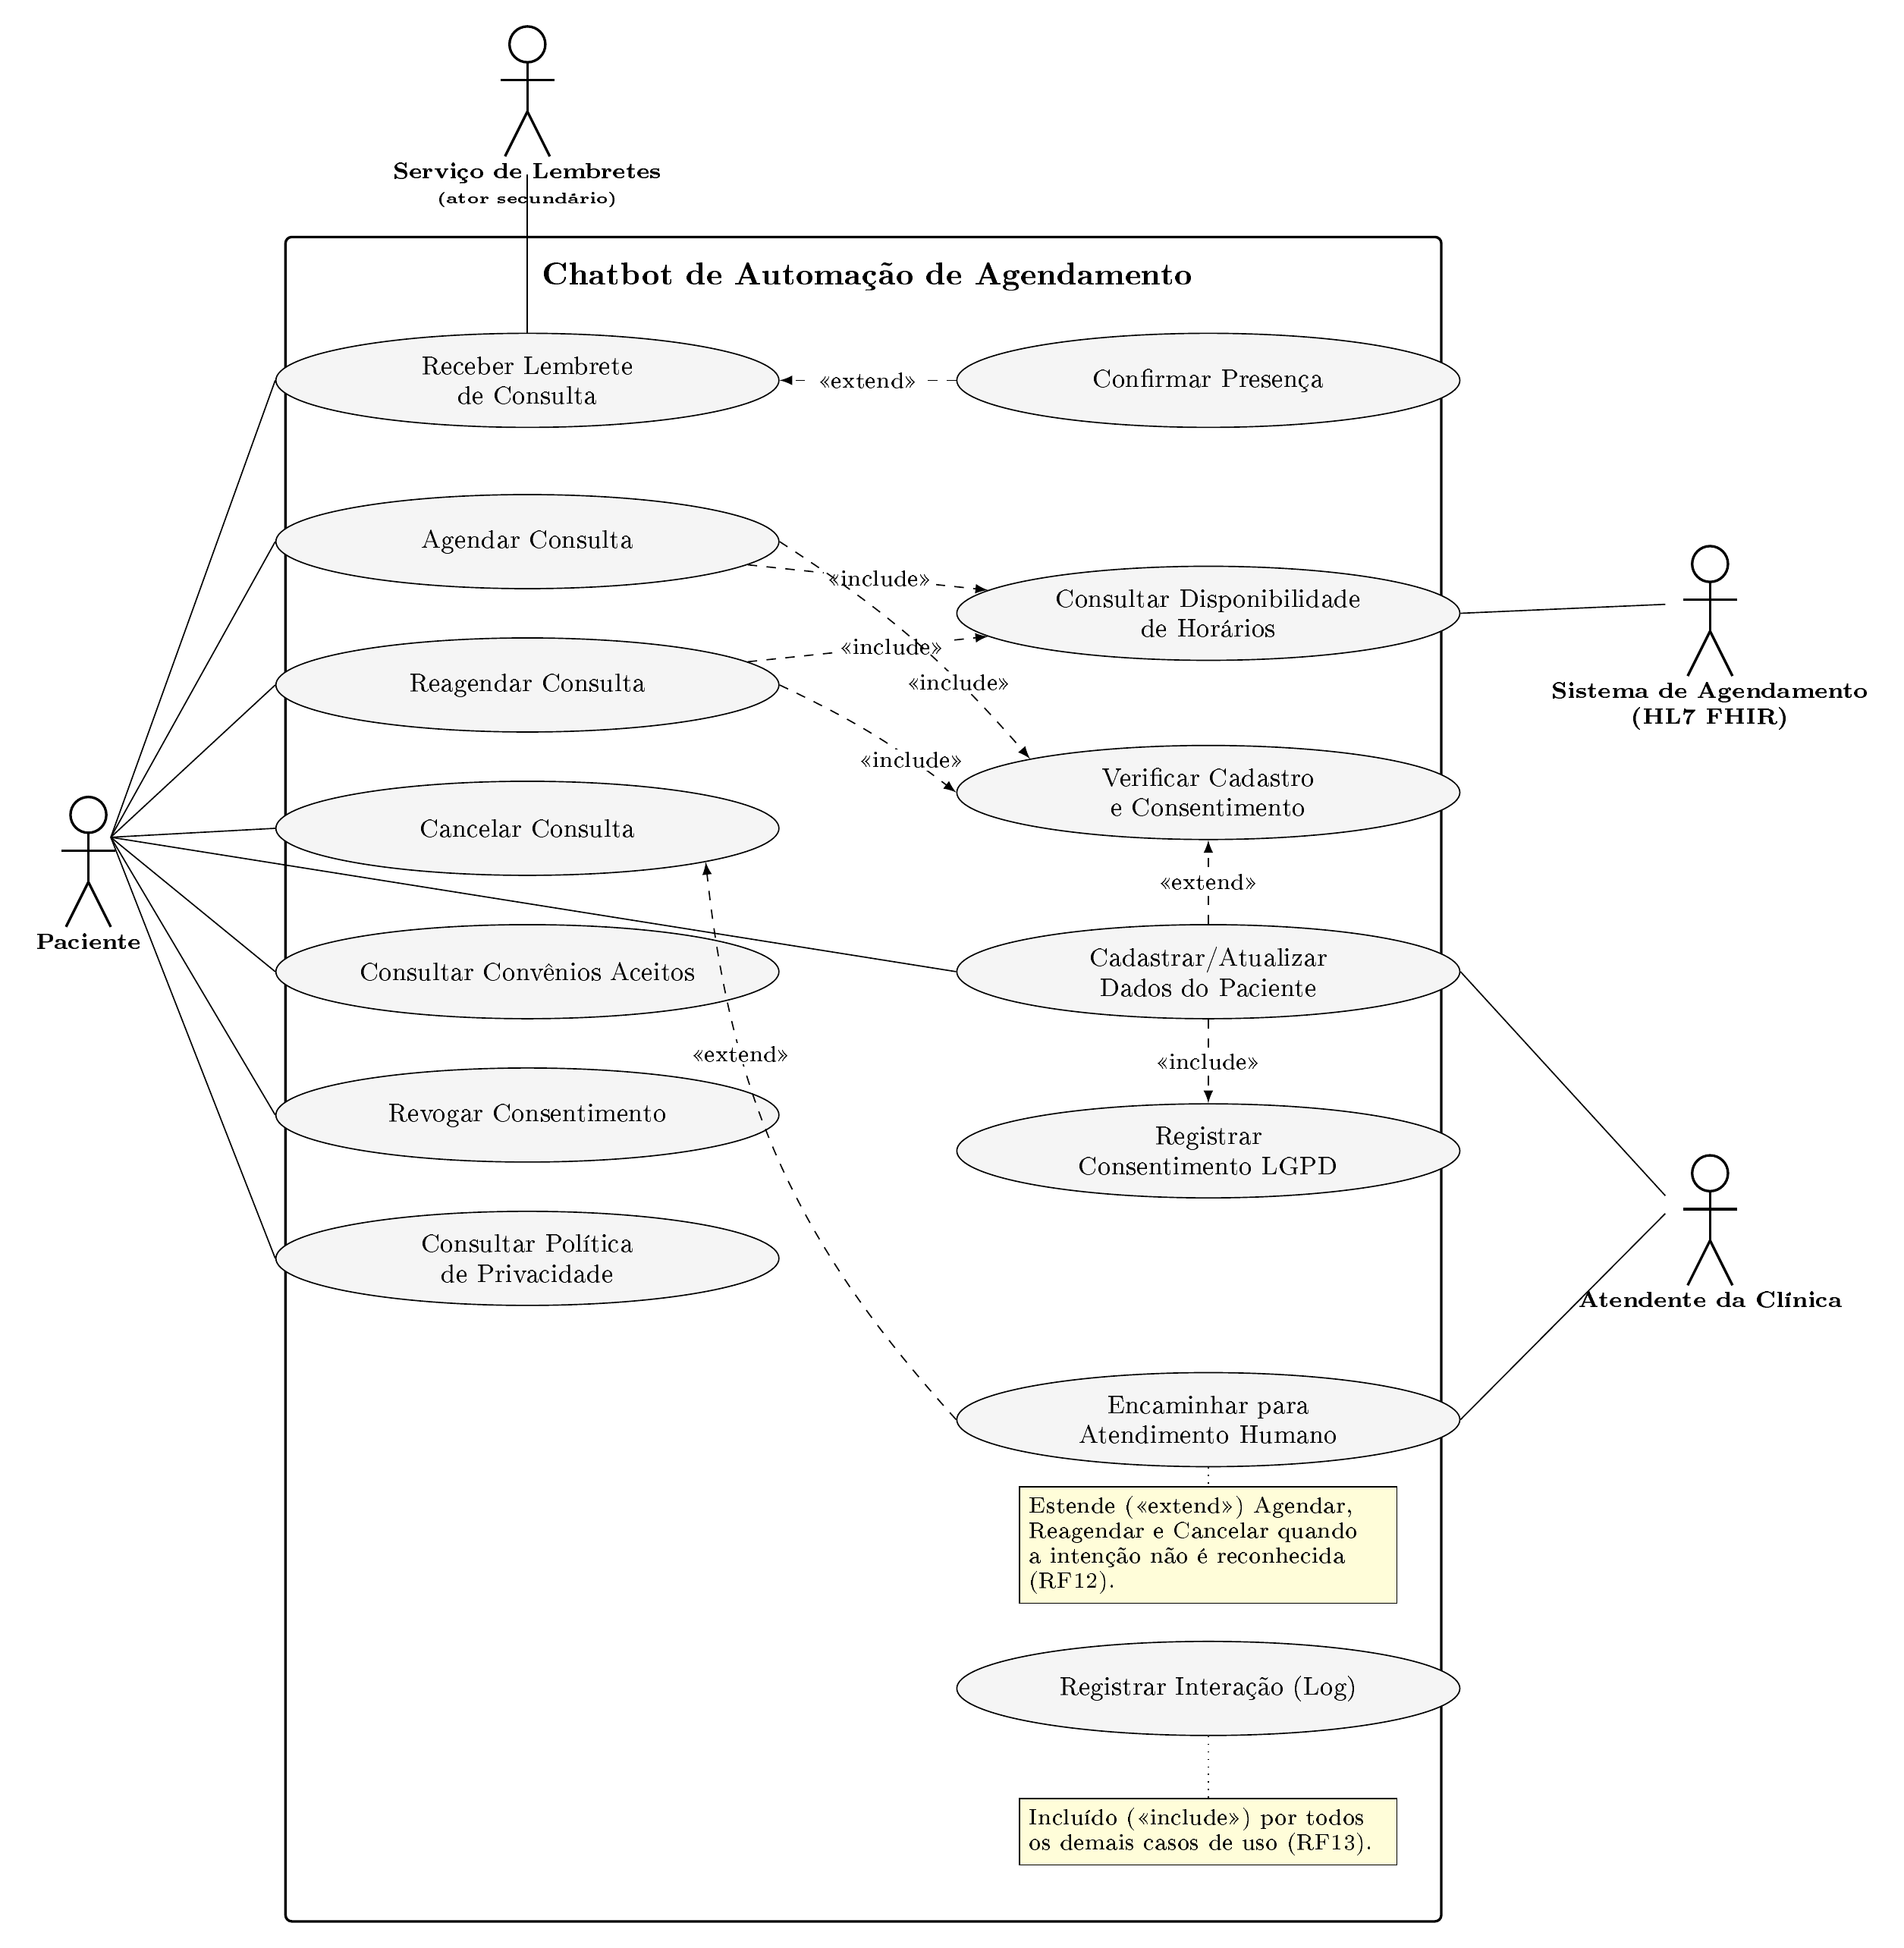
\includegraphics[width=0.95\textwidth]{fig_casos_de_uso.png}
    \label{fig:casos-uso}
    \vspace{0.2cm}
    \footnotesize{Fonte: Elaborado pelo autor (2026), com base na notação de Larman (2004) e OMG (2017).}
\end{figure}

\subsubsection{Diagrama de Atividades}

Os diagramas de atividades detalham o comportamento dinâmico de quatro fluxos: os dois considerados mais críticos para o cenário de pequenas e médias clínicas (seção~\ref{sec:procedimentos}), o agendamento de uma nova consulta e o cancelamento ou reagendamento de uma consulta já existente, e, complementarmente, o cadastro com consentimento e os lembretes. Segundo Sommerville (2016), diagramas de atividades são particularmente adequados para representar processos de negócio que envolvem decisões condicionais e paralelismo entre etapas, sendo, portanto, compatíveis com a natureza dos fluxos automatizados pelo chatbot proposto.

A Figura~\ref{fig:atividade-agendamento} apresenta o fluxo de agendamento de consulta. O processo inicia-se quando o paciente envia uma mensagem ao chatbot, que classifica a intenção (RF01) e extrai as entidades (RF02); se a confiança da classificação for inferior a 0,70, o atendimento é encaminhado a um atendente humano (RF12). Em seguida, o chatbot verifica se o paciente possui cadastro e consentimento ativos (RF10, RF11); caso não possua, o fluxo da Figura \ref{fig:cadastro} é executado antes de prosseguir. Caso a especialidade não tenha sido informada, o chatbot solicita-a ao paciente, para não oferecer horários de especialidades não desejadas. Com a especialidade definida, consulta a disponibilidade de horários (RF03). Não havendo horário, o paciente é informado e pode refazer a busca; havendo disponibilidade, o chatbot apresenta até três opções e solicita confirmação explícita antes de registrar o agendamento (RF04), o que reduz o risco de erros de interpretação da linguagem natural, limitação discutida na seção 2.1.1 deste trabalho. Se, no momento da confirmação, o horário já tiver sido reservado por outra pessoa, o agendamento é recusado e o paciente é avisado. Confirmado o agendamento, o sistema registra o recurso \textit{Appointment}, reserva o horário, programa o lembrete automático, se houver consentimento para essa finalidade (RF08), e envia a confirmação ao paciente, fluxo que operacionaliza a estratégia de redução de \textit{no-show} discutida por Brancewicz et al. (2025).

\begin{figure}[H]
    \centering
    \caption{Diagrama de atividades do fluxo de agendamento de consulta}
    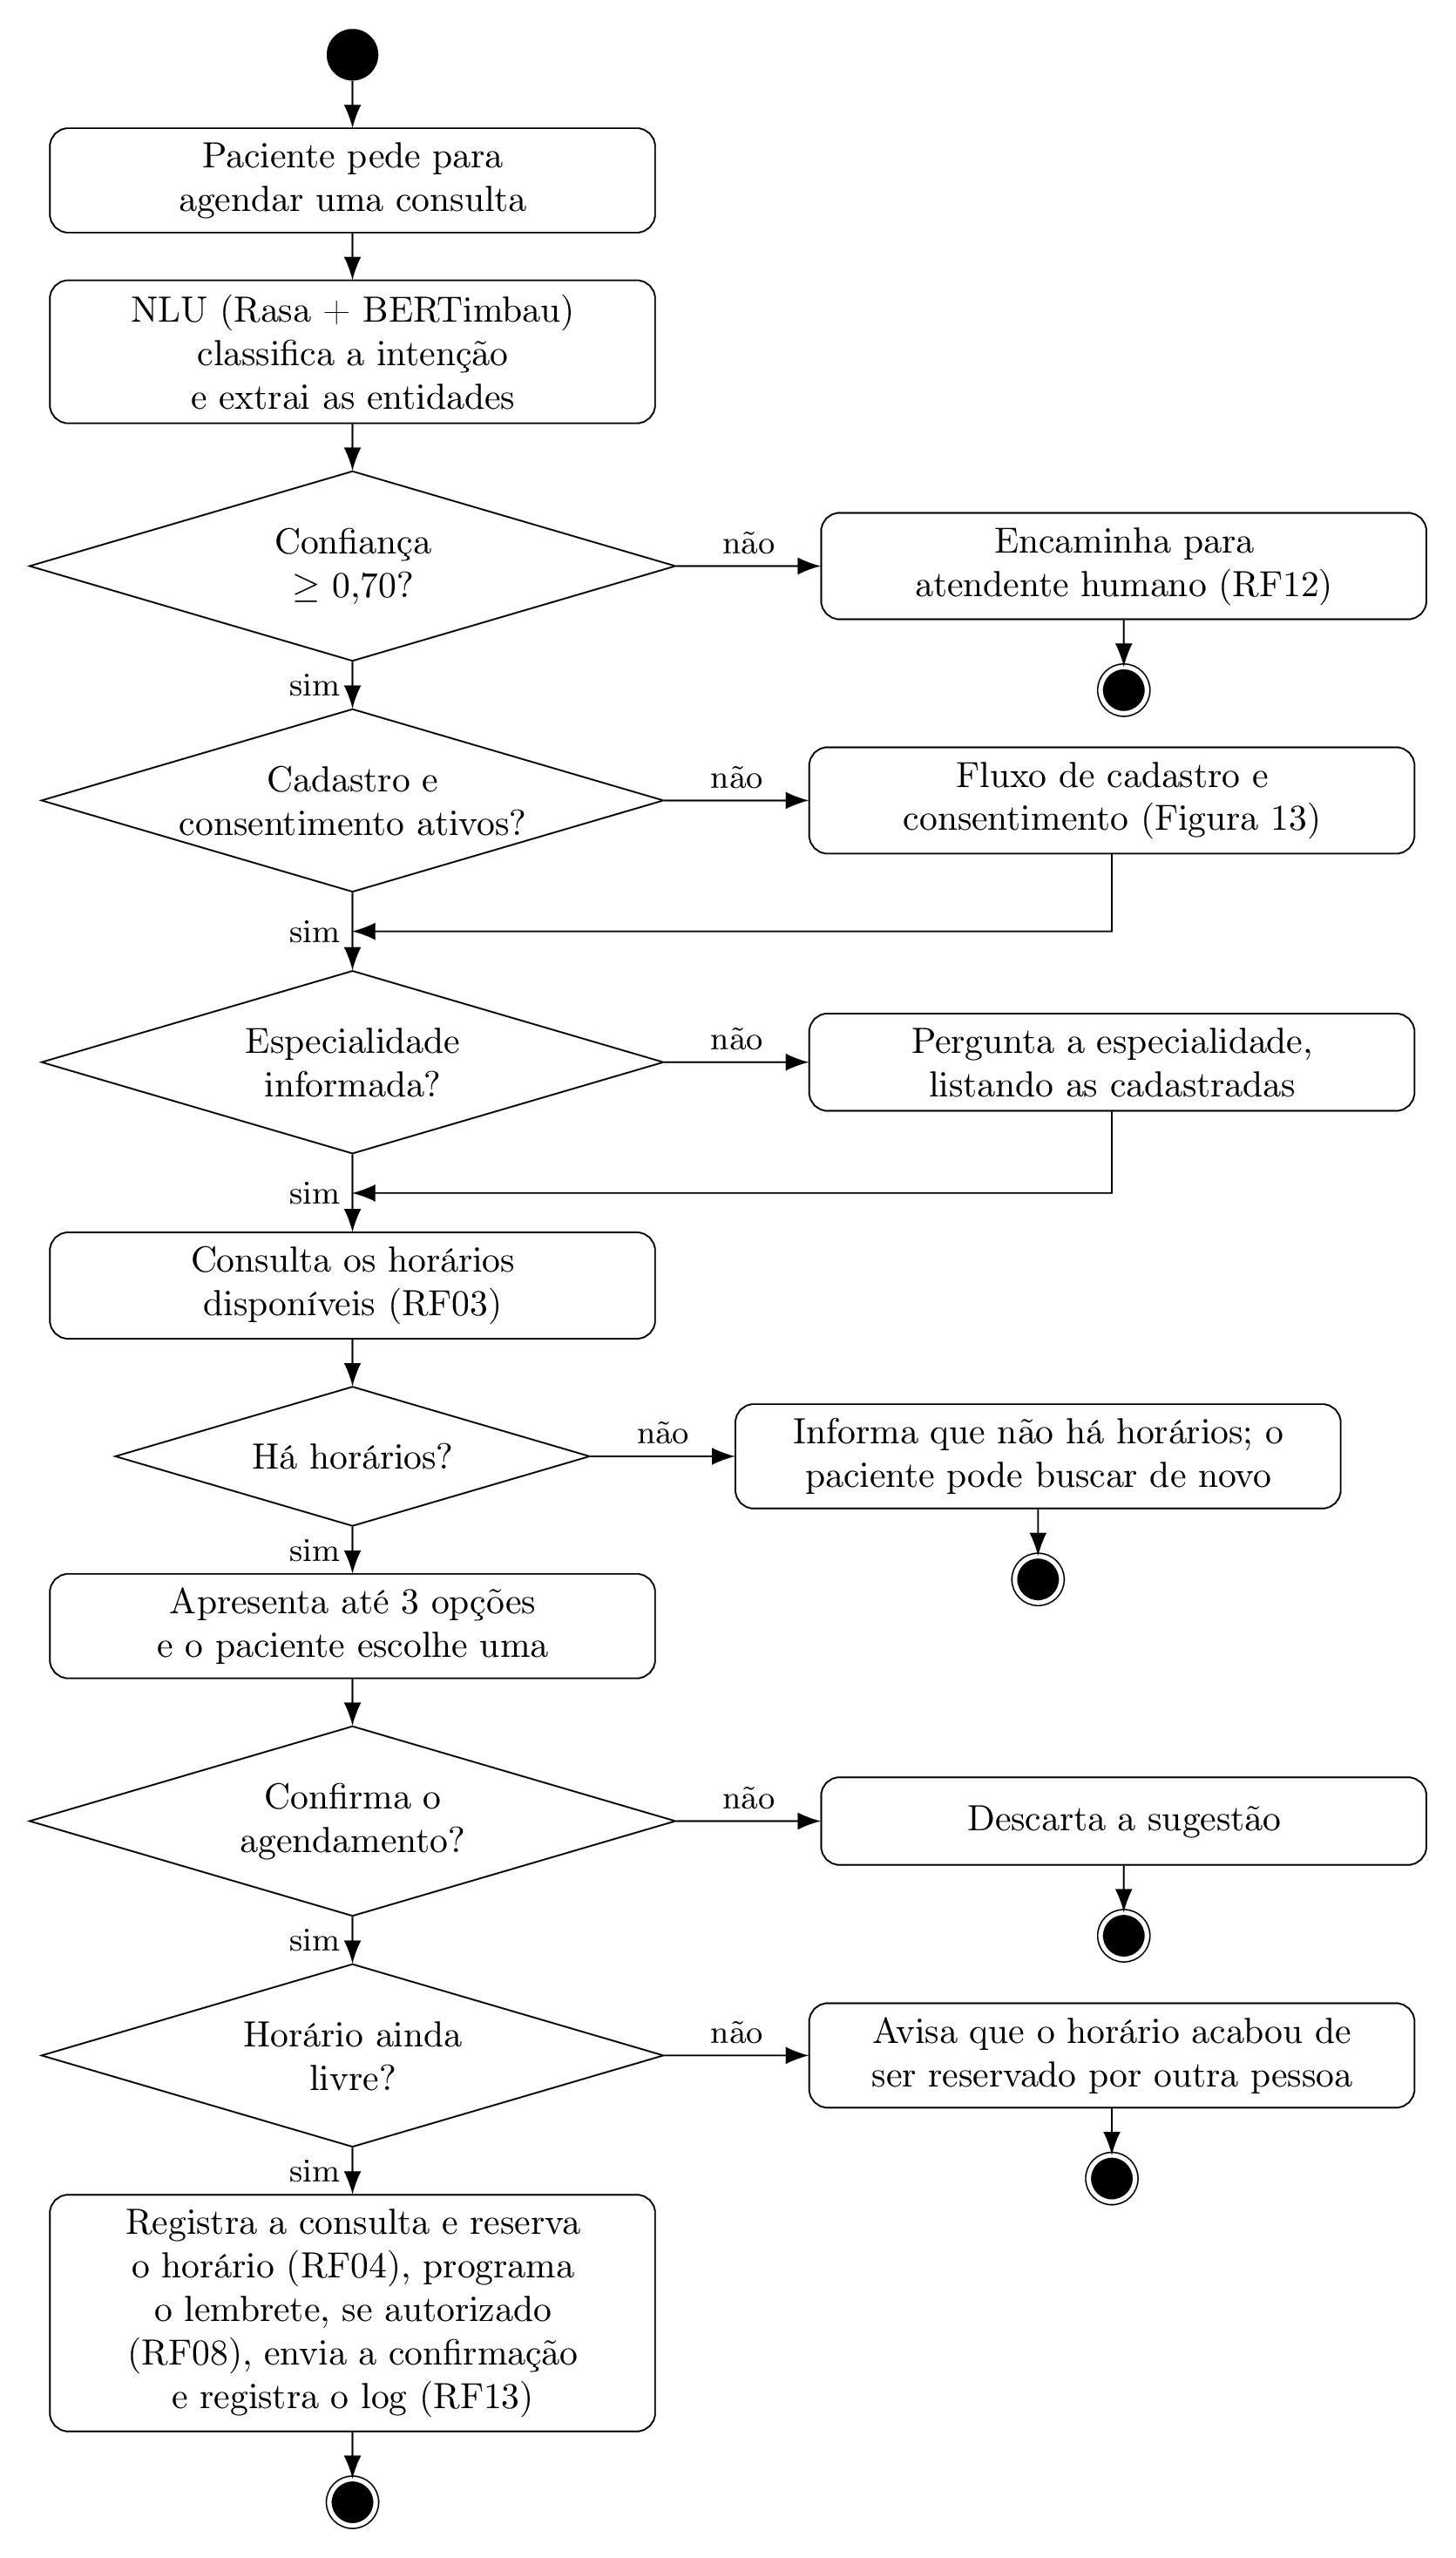
\includegraphics[height=0.78\textheight,keepaspectratio]{AtividadeAgendamentoo.png}\par
    \label{fig:atividade-agendamento}

    \vspace{0.2cm}
\end{figure}
\newpage
A Figura~\ref{fig:atividade-cancelamento} apresenta o fluxo de cancelamento e reagendamento, que compartilha com o fluxo anterior a etapa inicial de classificação de intenção. Em vez de solicitar um identificador, o sistema localiza as consultas ativas futuras do paciente (recurso \textit{Appointment}), identificado pelo seu canal de conversa; não havendo consulta ativa, o paciente é informado, e, havendo mais de uma, o chatbot as lista e pergunta qual deve ser cancelada ou remarcada. Havendo, o fluxo se ramifica conforme a intenção: no cancelamento (RF05), o chatbot mostra a consulta e pede confirmação, válida por cinco minutos, e só então marca a consulta como cancelada, mantida como histórico, libera o horário e anula os lembretes pendentes; no reagendamento (RF06), apresenta os horários disponíveis e, confirmada a escolha e verificado que o novo horário continua livre, reserva-o, libera o anterior e marca a consulta como reagendada. Em ambos os casos, o fluxo termina com a confirmação ao paciente e o registro da interação no log do sistema (RF13).

\begin{figure}[H]
    \centering
    \caption{Diagrama de atividades do fluxo de cancelamento e reagendamento de consulta}
    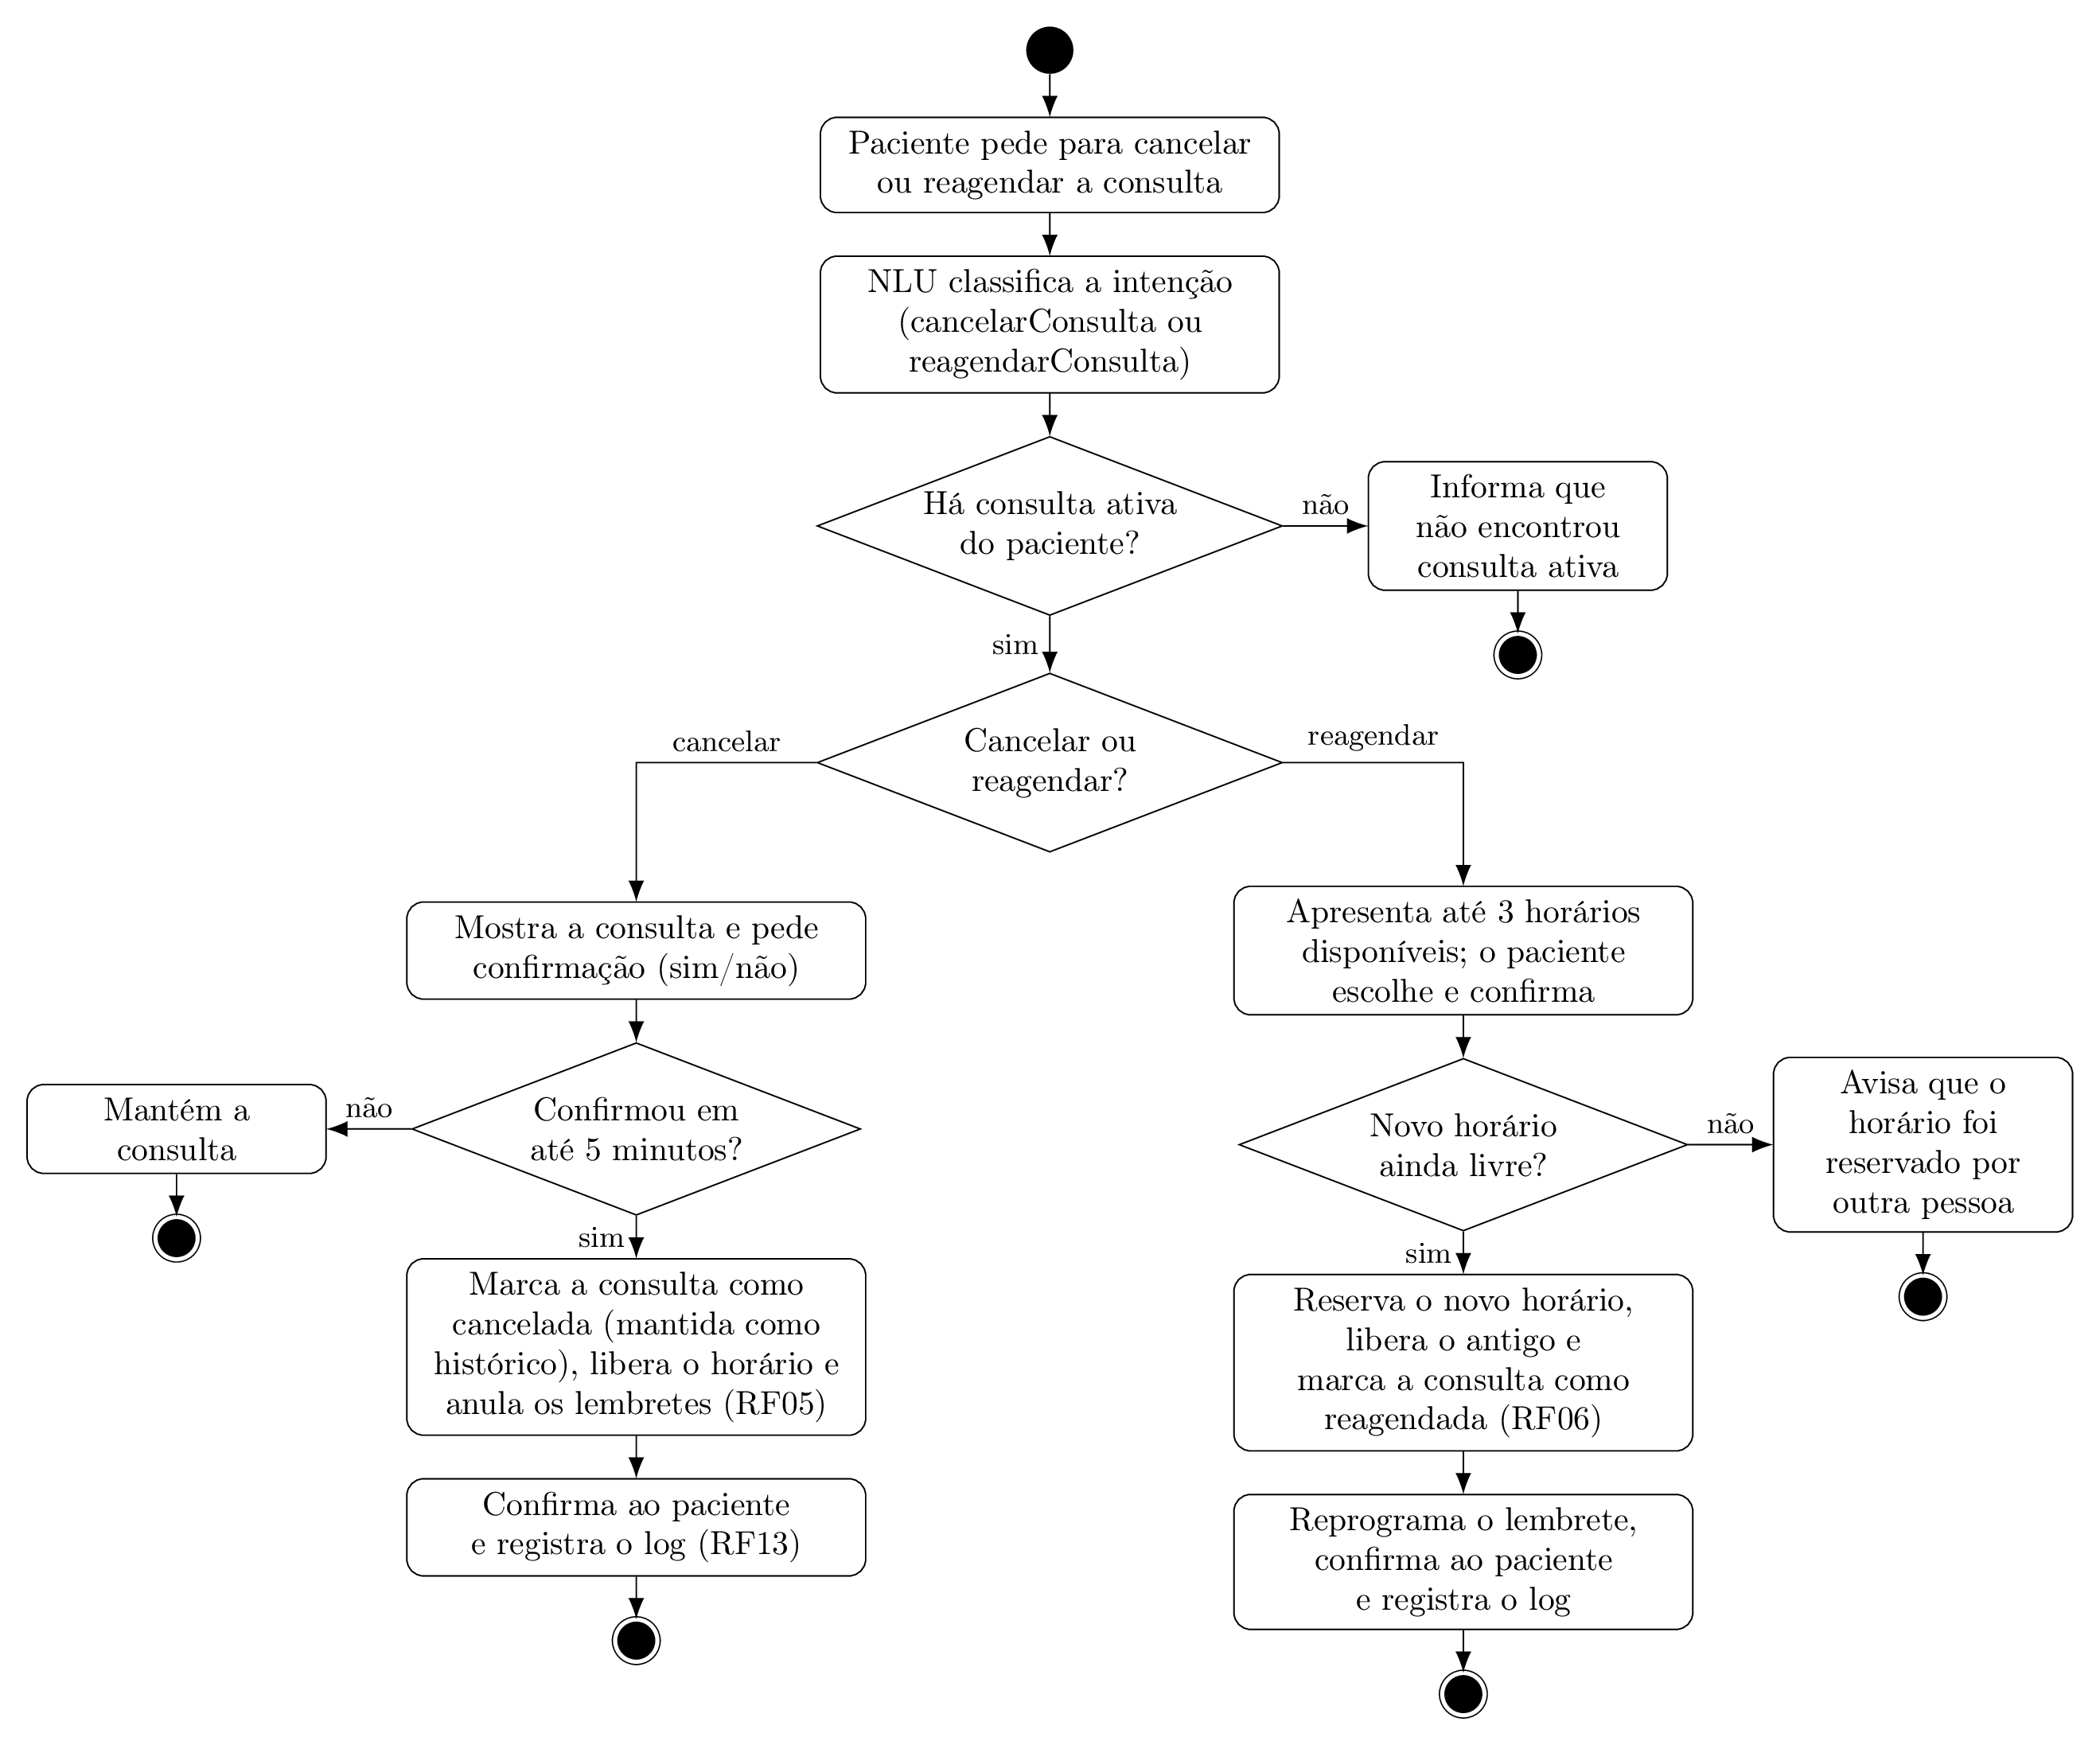
\includegraphics[width=\textwidth]{AtividadeCancelaa.png}\par
    \label{fig:atividade-cancelamento}

    \vspace{0.2cm}
\end{figure}

A Figura \ref{fig:cadastro} detalha o fluxo de cadastro e consentimento (RF10, RF11). O paciente que ainda não possui cadastro, ou que revogou o consentimento, é conduzido a um formulário cuja primeira etapa é a exibição do texto de consentimento, antes da coleta de qualquer dado pessoal. A recusa encerra o fluxo sem que nenhum dado seja gravado. Havendo aceite, o chatbot pergunta se o paciente deseja receber lembretes (finalidade opcional e separada), coleta nome, data de nascimento, telefone e convênio, validando cada resposta, e só então grava o paciente e os registros de consentimento, com a data e a hora do aceite. Ao final, o agendamento que estava pendente é retomado. Quando o cadastro já existe e apenas o consentimento foi revogado, os dados são reaproveitados e somente a autorização é solicitada novamente.

\begin{figure}[H]
    \centering
    \caption{Diagrama de atividades do fluxo de cadastro e consentimento}
    \label{fig:cadastro}
    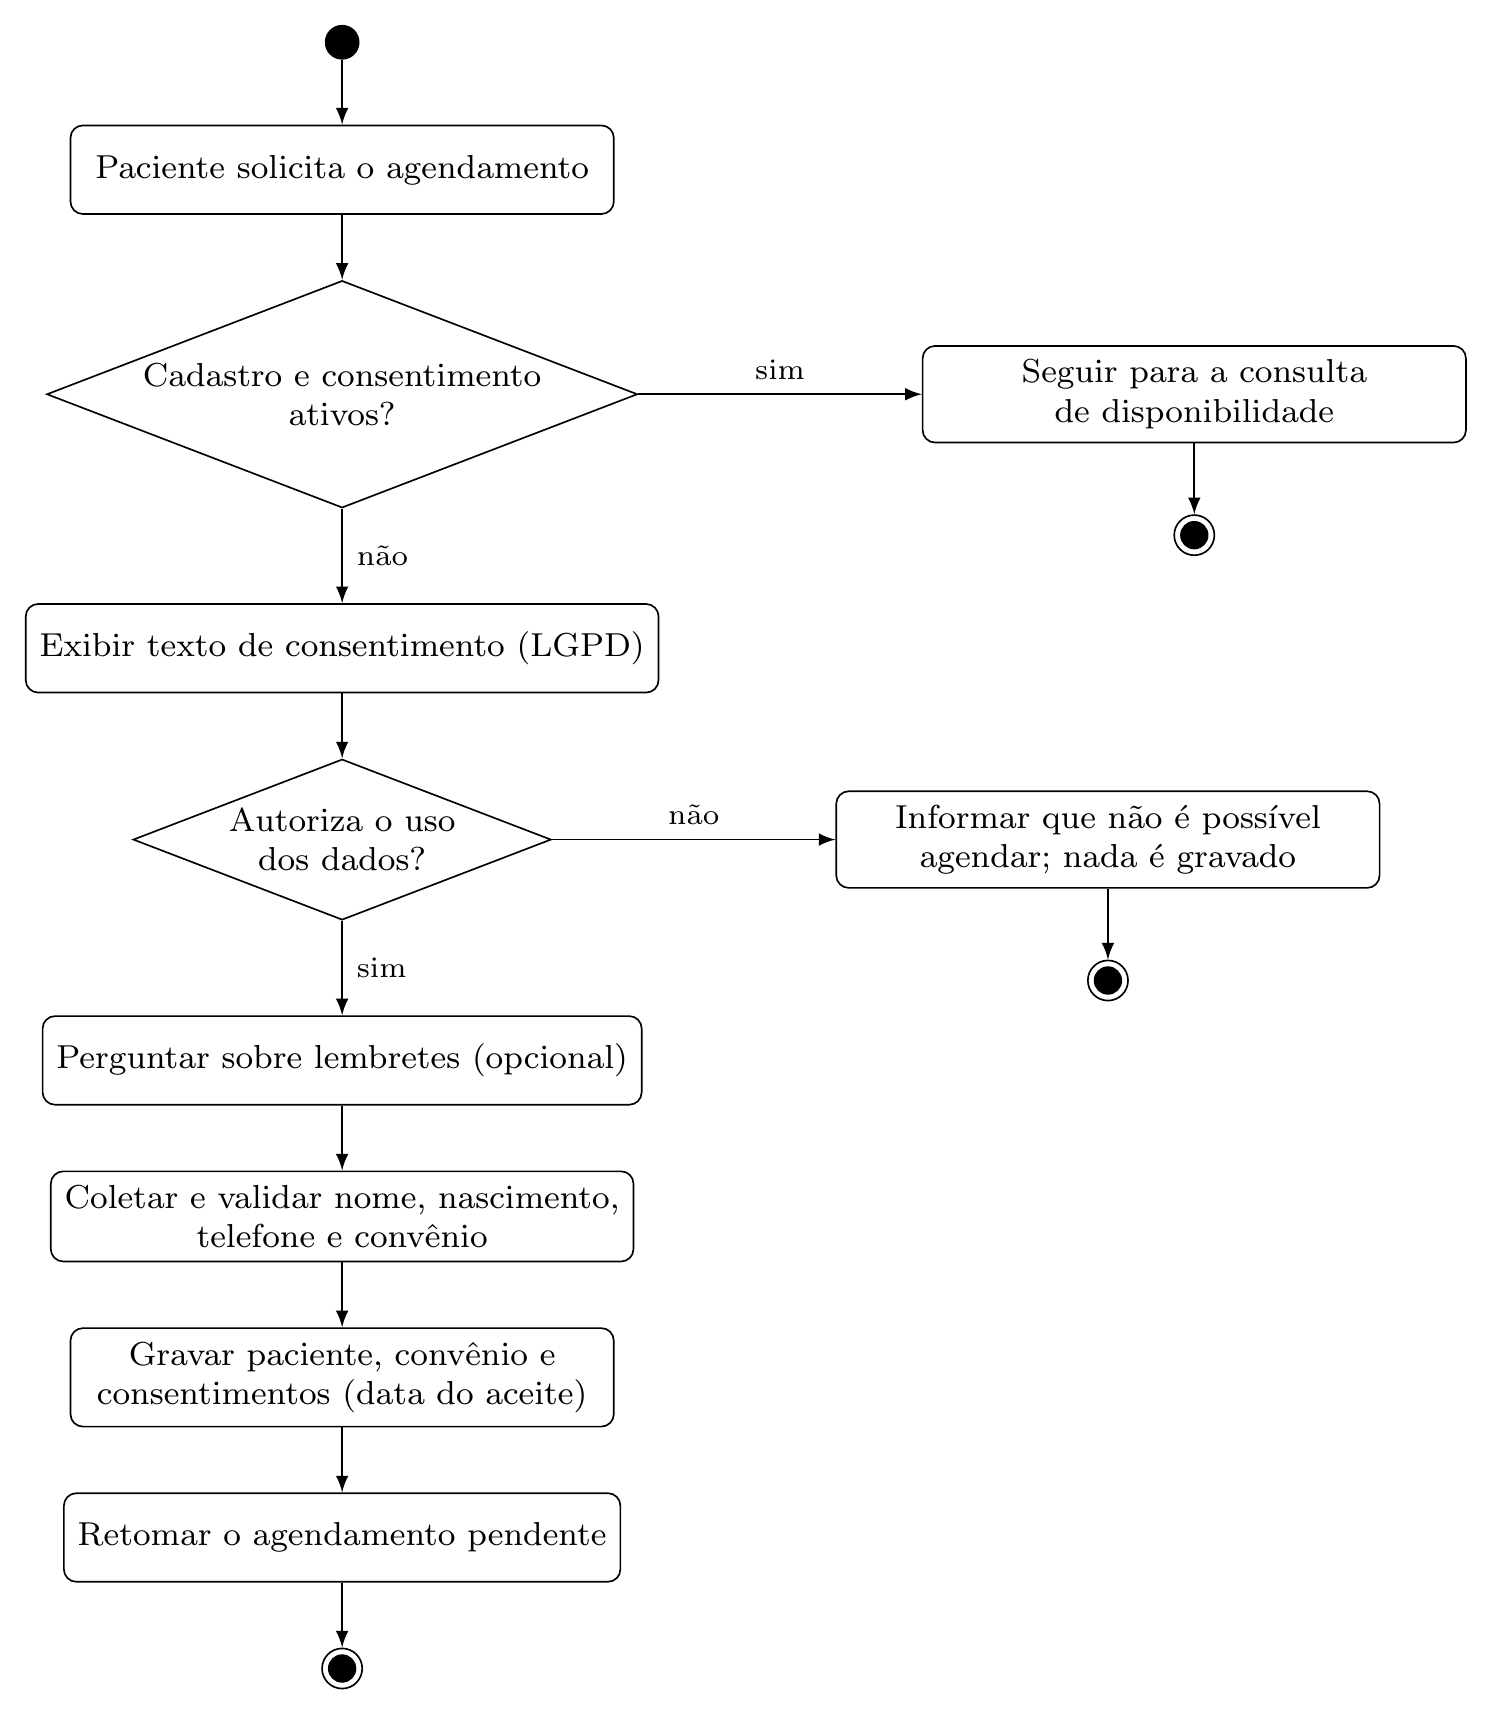
\includegraphics[width=0.8\textwidth]{fig_cadastro_consentimento.png}
    \vspace{0.2cm}
    \begin{center}
        \footnotesize Fonte: Elaborado pelo autor (2026).
    \end{center}
\end{figure}

A Figura \ref{fig:lembretes} apresenta o fluxo dos lembretes (RF08, RF09). O lembrete é programado no momento em que a consulta é confirmada, para 24 horas antes do horário agendado, e apenas se houver consentimento ativo para essa finalidade. Um serviço independente verifica periodicamente os lembretes vencidos e, antes de cada envio, confere se a consulta continua ativa, se o paciente está identificado no canal e se o consentimento continua vigente. O paciente confirma a presença respondendo ao lembrete; sem confirmação, um novo lembrete é enviado quando faltarem menos de 3 horas para a consulta. Lembretes enviados e não confirmados até a realização da consulta passam à situação ``ignorado''. O cancelamento ou o reagendamento da consulta, assim como a revogação do consentimento, interrompem os lembretes pendentes.

\begin{figure}[H]
    \centering
    \caption{Diagrama de atividades do fluxo de lembretes e confirmação de presença}
    \label{fig:lembretes}
    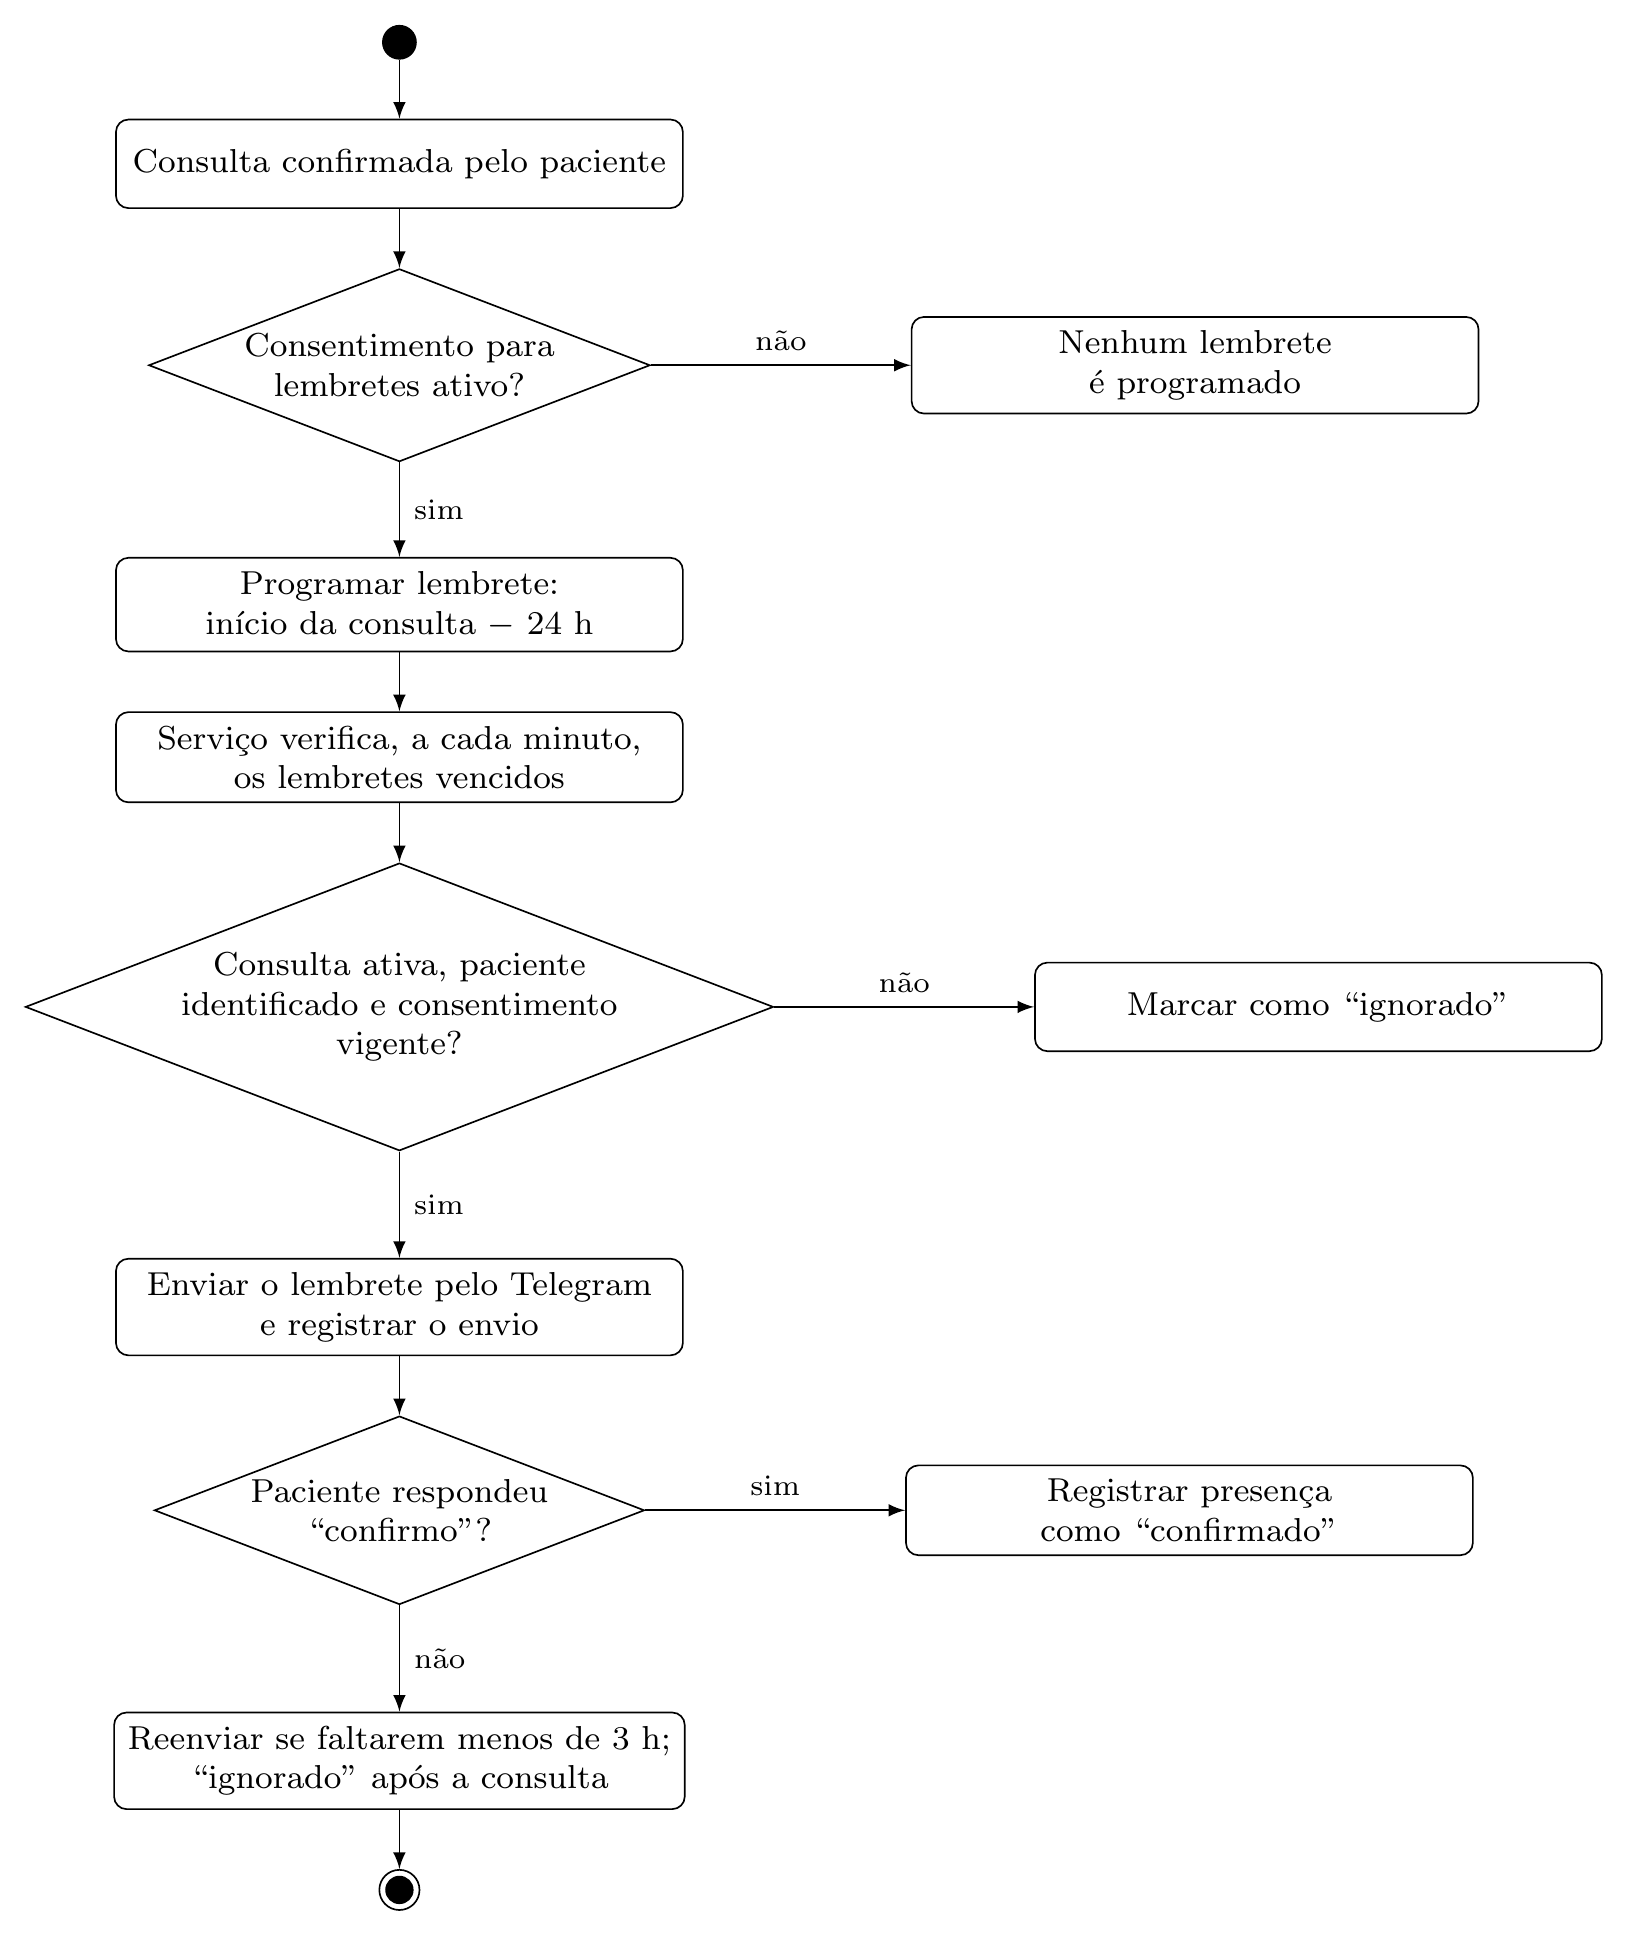
\includegraphics[width=0.8\textwidth]{fig_lembretes.png}
    \vspace{0.2cm}
    \begin{center}
        \footnotesize Fonte: Elaborado pelo autor (2026).
    \end{center}
\end{figure}

\subsubsection{Diagrama de Classes}

O diagrama de classes apresentado na Figura ~\ref{fig:diagrama-classes} corresponde à estrutura estática do sistema, elaborada com o propósito de organizar as principais abstrações de domínio identificadas no projeto. Conforme observa Larman (2004), um modelo de classes de análise não precisa representar todos os detalhes de implementação, cumprindo antes a função de consolidar o vocabulário do domínio e as relações estruturais entre as entidades.

As classes Paciente, Consulta, Médico e Horário representam o núcleo do domínio de agendamento e correspondem, respectivamente, aos recursos \textit{Patient}, \textit{Appointment}, \textit{Practitioner} e \textit{Slot} do padrão HL7 FHIR (BENDER; SARTIPI, 2013), o que reduz o esforço de mapeamento para uma futura integração com um servidor FHIR. Os atributos e as situações (\textit{status}) de cada classe são os mesmos do banco de dados implementado (seção 4.4). A classe ConsentimentoLGPD foi incluída como entidade própria, e não como um simples atributo booleano do Paciente, em razão da exigência legal de que o consentimento para tratamento de dados sensíveis de saúde seja auditável, com finalidade, base legal e datas de concessão e de revogação (art. 7º e art. 11 da LGPD), conforme discutido na seção 2.7.1. A parte superior do diagrama mostra os componentes de execução: o canal do Telegram encaminha as mensagens ao assistente do Rasa, responsável pela compreensão de linguagem natural e pelo gerenciamento do diálogo (seção 2.3), que aciona o servidor de ações, onde ficam as regras de negócio e o acesso ao banco de dados; o serviço de lembretes opera de forma independente sobre a classe Lembrete. Essa separação mantém o baixo acoplamento entre subsistemas (SOMMERVILLE, 2016). Por fim, a classe Handoff registra os chamados de atendimento humano e não se associa ao Paciente, pois a conversa pode ser encaminhada antes de o paciente se identificar.

\begin{figure}[H]
    \centering
    \caption{Diagrama de classes do sistema}
    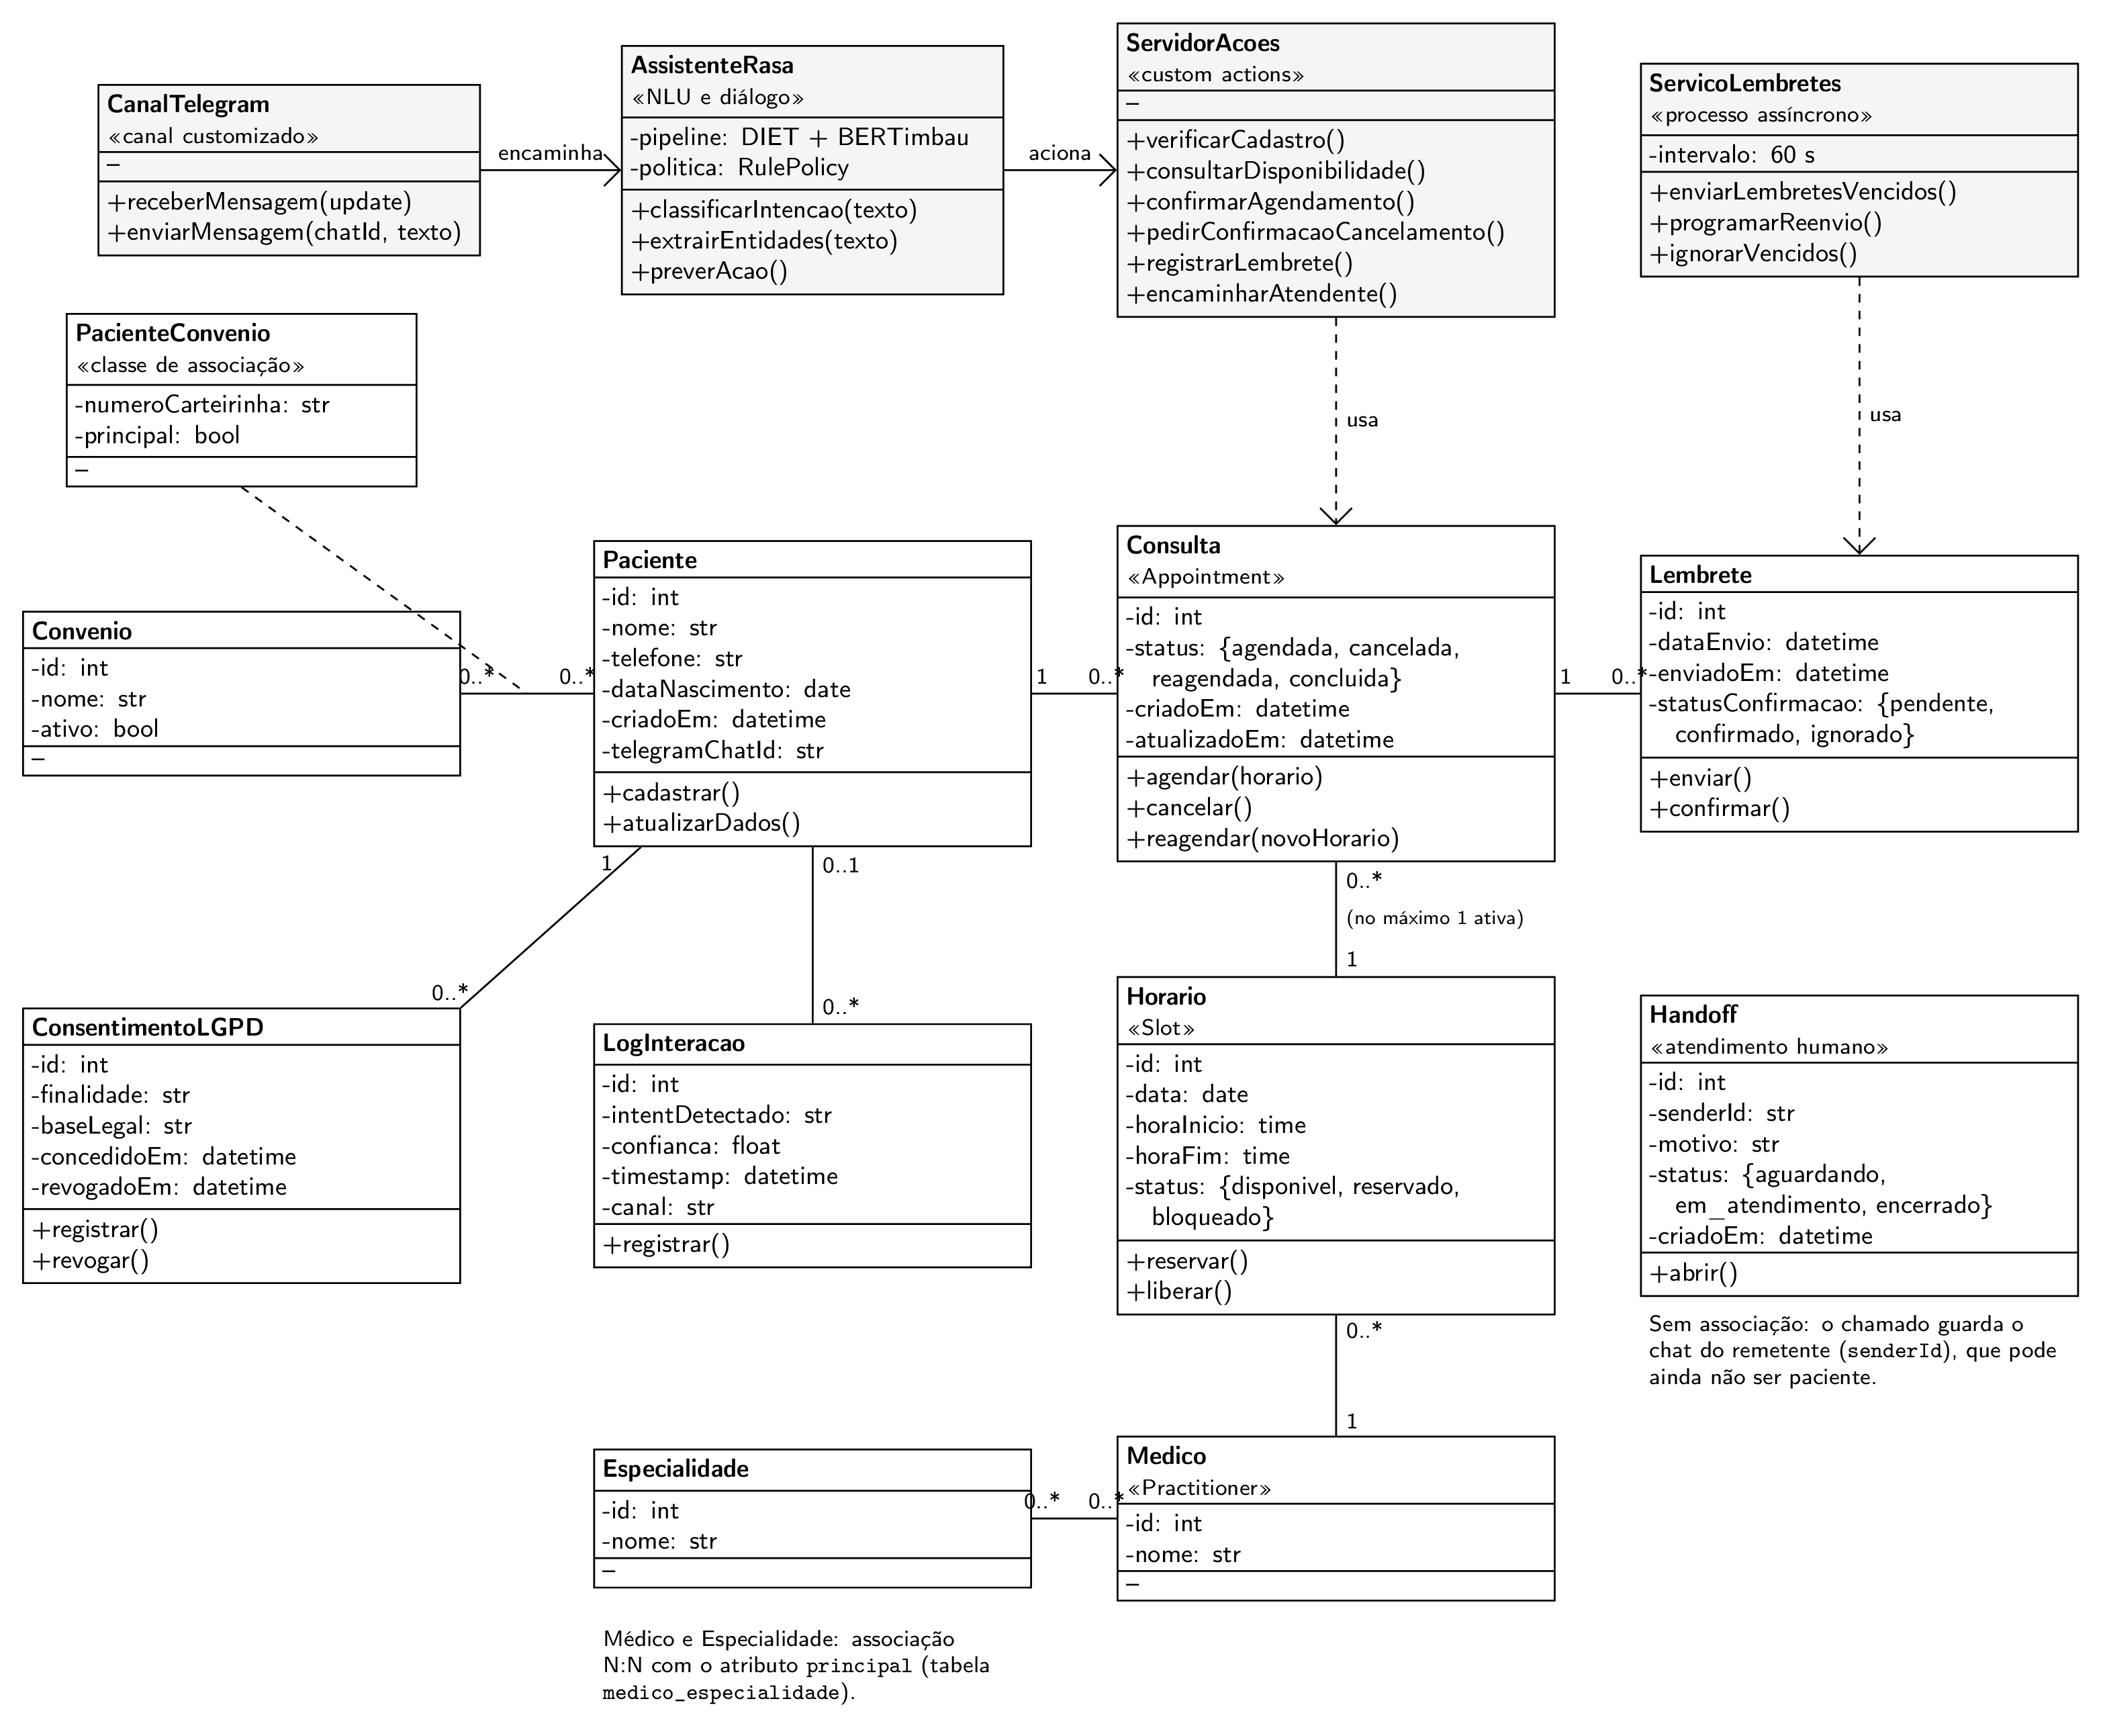
\includegraphics[angle=90,width=\textwidth]{DiagramaClasses (2).png}\par
    \label{fig:diagrama-classes}
    \vspace{0.2cm}
    \footnotesize{Fonte: Elaborado pelo autor (2026), com base em Larman (2004) e Bender e Sartipi (2013).}
\end{figure}

\subsubsection{Diagrama de Sequência}

Enquanto os diagramas de atividades apresentados na seção 4.3.2 descrevem o fluxo lógico de decisões de cada processo administrativo, os diagramas de sequência complementam essa visão ao detalhar a ordem temporal das trocas de mensagens entre os elementos que compõem a arquitetura do sistema, o paciente, o Rasa (compreensão de linguagem natural e gerenciamento de diálogo), o servidor de ações, responsável pelas regras de negócio e pelo acesso aos dados, e o banco de dados, cujo modelo lógico é apresentado na seção 4.4. Segundo Larman (2004) e a especificação da OMG (2017), o diagrama de sequência é particularmente adequado para representar cenários de interação nos quais a ordem das mensagens trocadas entre objetos é determinante para a correção do comportamento do sistema, sendo por isso utilizado neste trabalho para detalhar os dois fluxos administrativos já modelados por diagramas de atividades.

A Figura~\ref{fig:diagrama-sequencia-agenda} apresenta o diagrama de sequência do fluxo de agendamento de consulta. O processo inicia-se com o envio da mensagem do paciente ao Rasa, que classifica a intenção e extrai as entidades (RF01, RF02) e aciona o servidor de ações para verificar o cadastro e o consentimento do paciente; na ausência deles, executa-se antes o fluxo de cadastro. Em seguida, o servidor de ações consulta no banco de dados os horários disponíveis da especialidade (RF03), e o paciente escolhe uma das opções e confirma o agendamento. A reserva é feita por uma atualização condicional do horário, que só tem efeito se ele ainda estiver disponível: havendo sucesso, a consulta é registrada na mesma transação (RF04) e o lembrete é programado (RF08); caso contrário, a transação é desfeita e o paciente é avisado de que o horário acabou de ser reservado por outra pessoa, mecanismo que, somado ao índice único parcial, impede o duplo agendamento. O diagrama evidencia ainda o registro complementar na tabela de log de interações, atendendo ao requisito de auditoria estabelecido pelo RF13.

\begin{figure}[H]
    \centering
    \caption{Diagrama de sequência do fluxo de agendamento de consulta}
    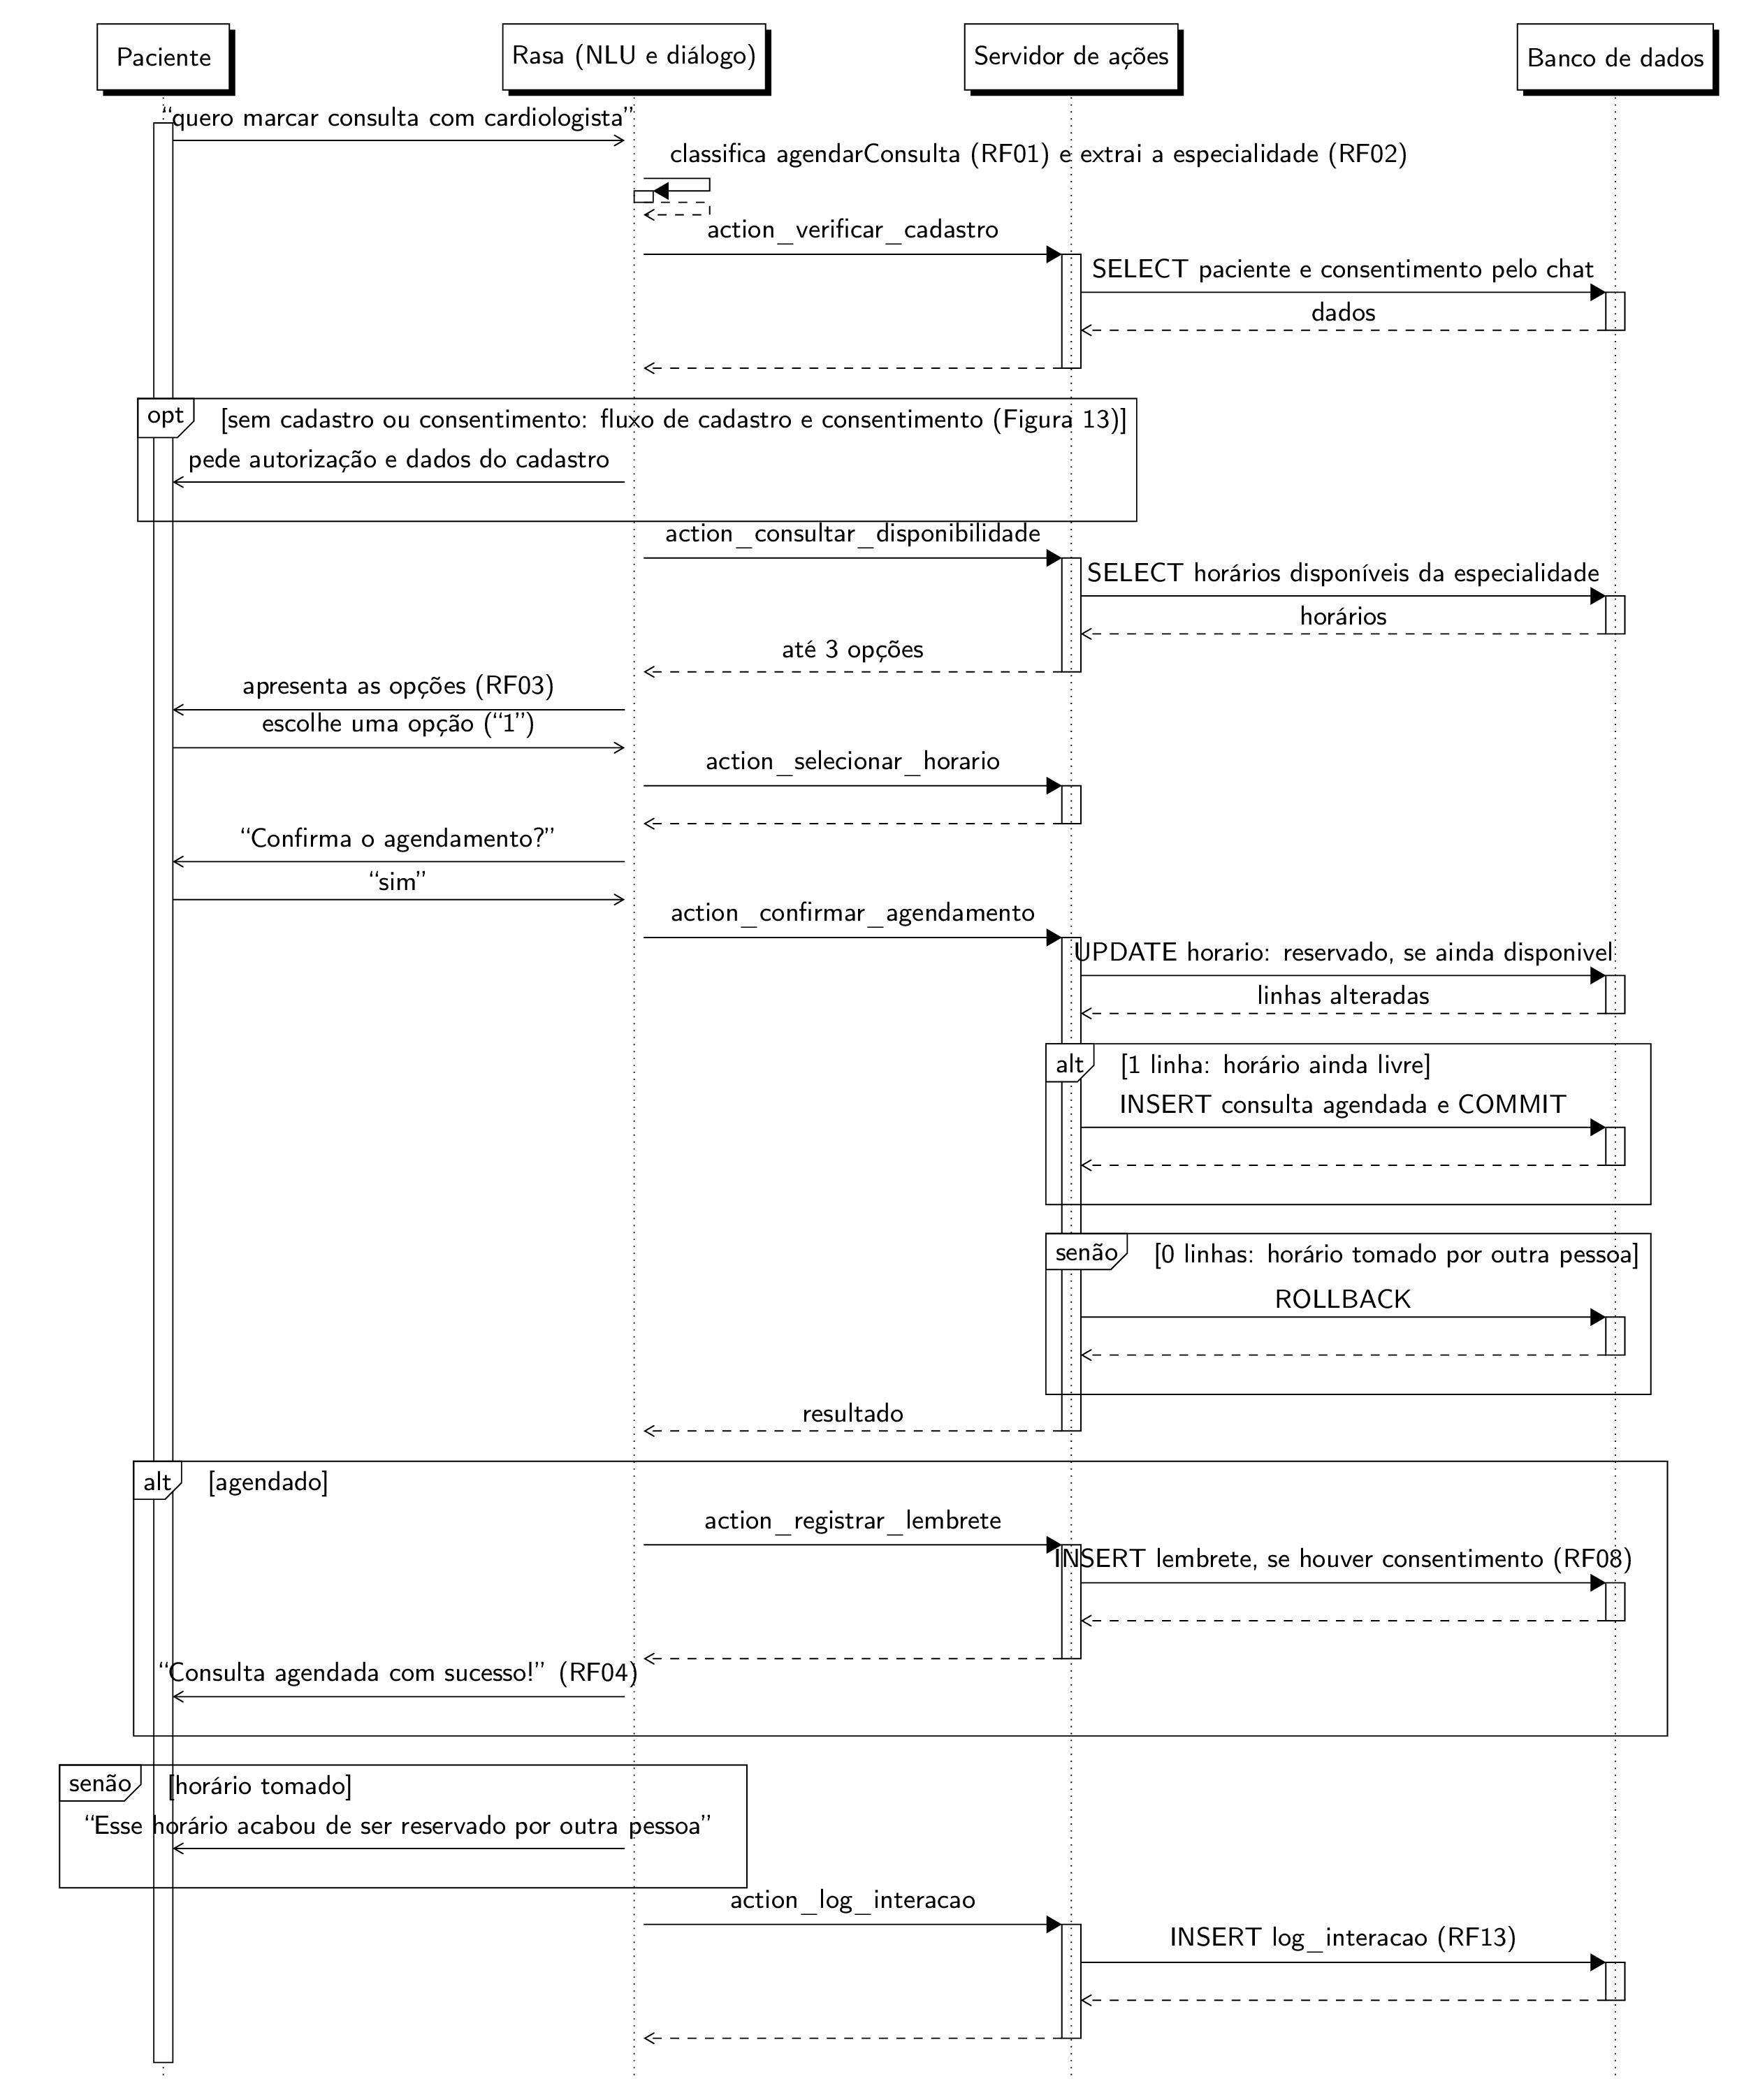
\includegraphics[width=\textwidth,height=0.8\textheight,keepaspectratio]{DiagramaAgendaCorrigida.png}\par
    \label{fig:diagrama-sequencia-agenda}
    \vspace{0.2cm}
    \footnotesize{Fonte: Elaborado pelo autor (2026), com base na notação de Larman (2004) e OMG (2017).}
\end{figure}

A Figura~\ref{fig:diagrama-sequencia-cancela} apresenta o diagrama de sequência do cancelamento e do reagendamento. No cancelamento (RF05), o servidor de ações localiza as consultas ativas futuras do paciente (havendo mais de uma, o paciente escolhe qual) e o chatbot pede confirmação explícita; confirmada a operação, a consulta é marcada como cancelada e mantida como histórico, o horário é liberado e os lembretes pendentes são anulados, tudo em uma única transação. No reagendamento (RF06), após a escolha e a confirmação do novo horário, o servidor de ações reserva primeiro o novo horário, com a mesma atualização condicional do agendamento, e só então libera o anterior, anula os lembretes pendentes e atualiza a consulta, mantendo o mesmo identificador; um novo lembrete é programado em seguida. Em ambos os casos, o registro da interação no log é a etapa final comum, reforçando o requisito RF13.

\begin{figure}[H]
    \centering
    \caption{Diagrama de sequência do fluxo de cancelamento e reagendamento de consulta}
    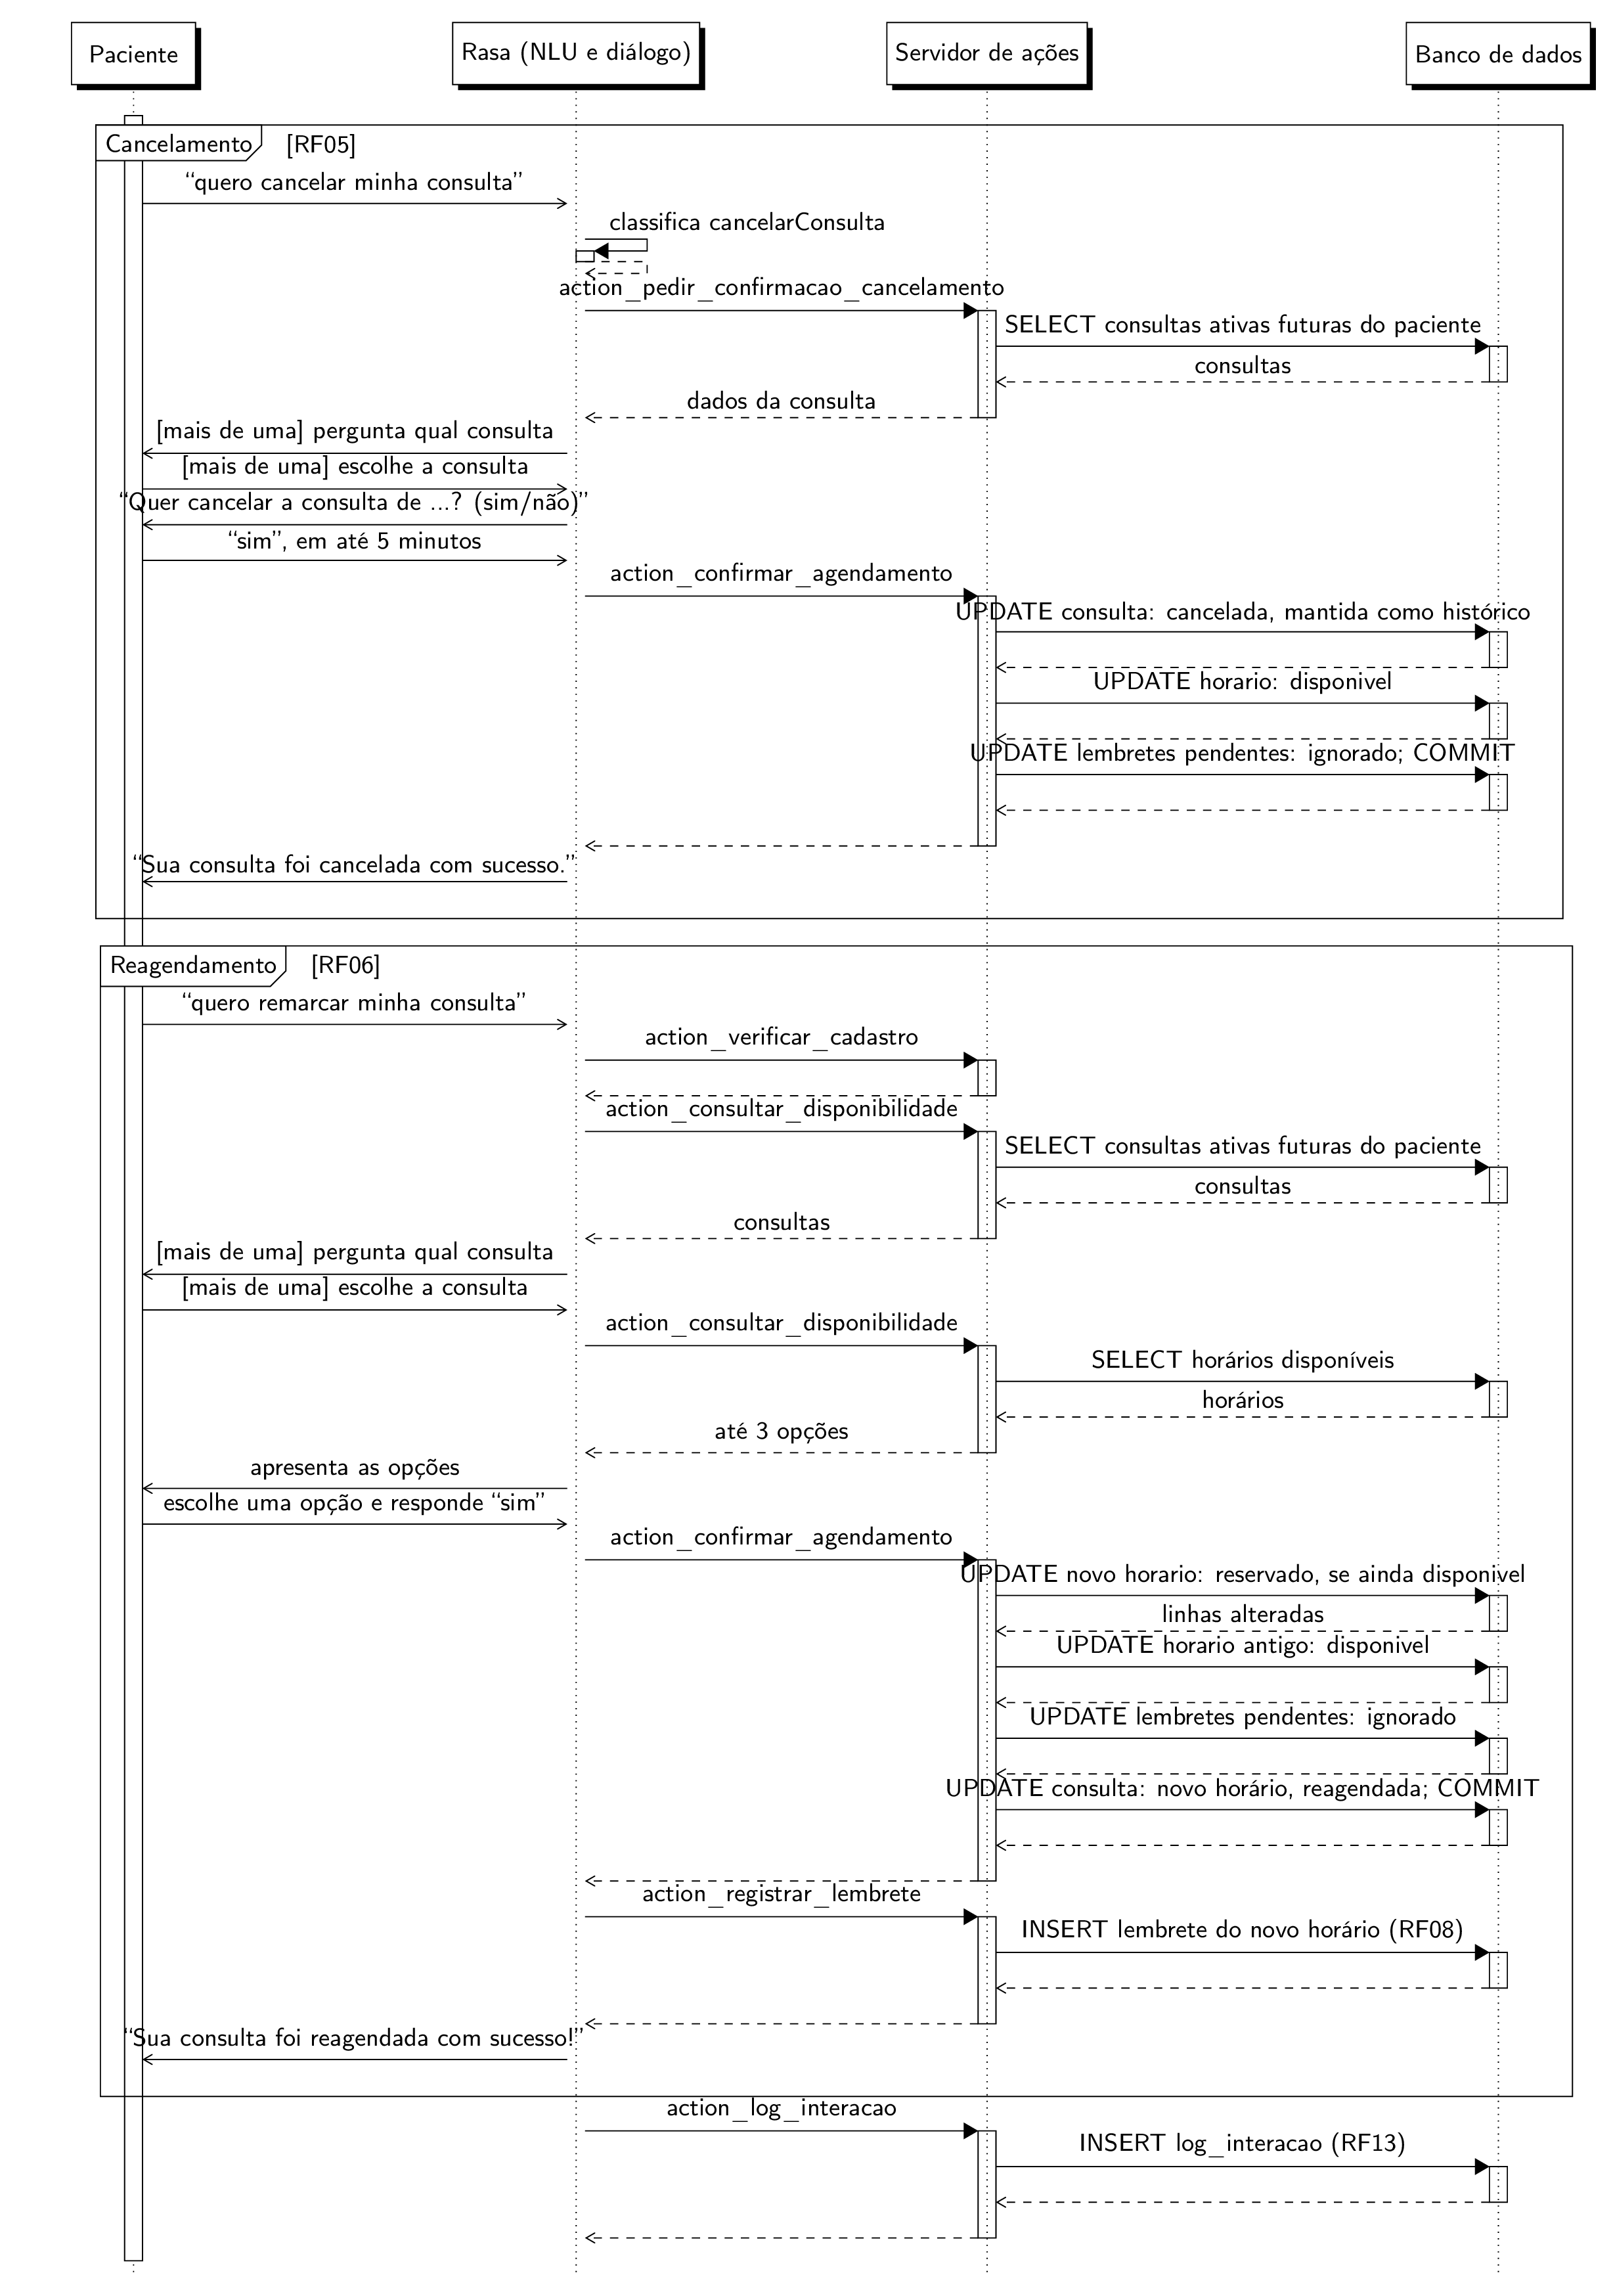
\includegraphics[width=\textwidth,height=0.8\textheight,keepaspectratio]{DiagragmaCancelaCorrigida.png}\par
    \label{fig:diagrama-sequencia-cancela}
    \vspace{0.2cm}
    \footnotesize{Fonte: Elaborado pelo autor (2026), com base na notação de Larman (2004) e OMG (2017).}
\end{figure}

\newpage

\subsection{Modelagem de Banco de Dados}

Esta seção apresenta a modelagem dos dados do protótipo em três níveis de abstração progressivos: conceitual, lógico e físico, seguindo a metodologia clássica de projeto de banco de dados descrita por Heuser (2009) e Elmasri e Navathe (2016), segundo a qual o modelo conceitual captura as entidades do domínio e seus relacionamentos independentemente de qualquer tecnologia de implementação, o modelo lógico traduz essas entidades para o modelo relacional (tabelas, chaves e restrições), e o dicionário de dados formaliza o significado e as regras de cada campo do esquema físico.

\subsubsection{Modelo Conceitual (MER)}

O Modelo de Entidade-Relacionamento (MER) do protótipo é composto por nove entidades, elaboradas a partir dos processos administrativos definidos na seção~\ref{sec:procedimentos} e dos recursos do padrão HL7 FHIR discutidos na seção 2.6. As entidades \textit{Paciente}, \textit{Horário} e \textit{Consulta} correspondem, respectivamente, aos recursos \textit{Patient}, \textit{Slot} e \textit{Appointment} do FHIR (BENDER; SARTIPI, 2013), enquanto \textit{Especialidade} e \textit{Convênio} foram destacadas como entidades independentes para evitar a repetição de atributos textuais, decisão retomada na modelagem lógica. As entidades \textit{ConsentimentoLGPD} e \textit{LogInteração} não decorrem do padrão FHIR, mas de requisitos legais e de auditoria específicos deste trabalho (RF11 e RF13, respectivamente). A entidade \textit{Lembrete} registra o envio e a confirmação dos lembretes automáticos exigidos pelos RF08 e RF09, permitindo rastrear se cada lembrete foi confirmado, ignorado ou está pendente. Cada lembrete registra, além da situação de confirmação, o momento programado para o envio e o momento em que o envio de fato ocorreu, o que permite distinguir lembretes agendados, enviados e confirmados.

Os relacionamentos identificados e suas cardinalidades são:

\begin{itemize}
    \item \textbf{Convênio (0,N) --- (0,N) Paciente}: um paciente pode estar vinculado a mais de um convênio simultaneamente (ex.: plano de saúde e plano odontológico), e um convênio cobre vários pacientes.
    \item \textbf{Especialidade (0,N) --- (0,N) Médico}: um médico pode atuar em mais de uma especialidade, situação comum em clínicas de pequeno e médio porte nas quais o mesmo profissional atende, por exemplo, Clínica Geral e Endocrinologia; e uma especialidade agrupa vários médicos.
    \item \textbf{Médico (1,1) --- (0,N) Horário}: um médico disponibiliza vários horários; cada horário pertence a um único médico;
    \item \textbf{Horário (1,1) --- (0,N) Consulta}: um horário pode estar associado a várias consultas ao longo do tempo (histórico de canceladas e concluídas), mas a no máximo uma consulta \textit{ativa}, restrição que garante a inexistência de duplo agendamento (RF04);
    \item \textbf{Paciente (1,1) --- (0,N) Consulta}: um paciente pode agendar várias consultas ao longo do tempo;
    \item \textbf{Paciente (1,1) --- (0,N) ConsentimentoLGPD}: um paciente pode conceder mais de um registro de consentimento, para diferentes finalidades (art. 7º, LGPD);
    \item \textbf{Consulta (1,1) --- (0,N) Lembrete}: uma consulta pode gerar mais de um lembrete ao longo do tempo (ex.: reenvio em caso de não confirmação), e cada lembrete está vinculado a exatamente uma consulta;
    \item \textbf{Paciente (0,1) --- (0,N) LogInteração}: uma interação pode ocorrer antes da identificação do paciente, daí a cardinalidade mínima zero do lado do log.
\end{itemize}

Os dois relacionamentos muitos-para-muitos: Médico–Especialidade e Paciente–Convênio, não podem ser representados por uma simples chave estrangeira no modelo relacional; sua tradução exige a criação de entidades associativas (\textit{MedicoEspecialidade} e \textit{PacienteConvenio}), detalhadas na seção 4.4.2, de modo que o esquema físico totaliza onze tabelas de domínio, às quais se soma a tabela \texttt{handoff}, que registra os chamados de atendimento humano.

A Figura \ref{fig:mer-conceitual} apresenta o MER correspondente, elaborado com notação de cardinalidade mínima e máxima.

\begin{figure}[H]
    \centering
    \caption{Modelo conceitual (MER) do protótipo}
    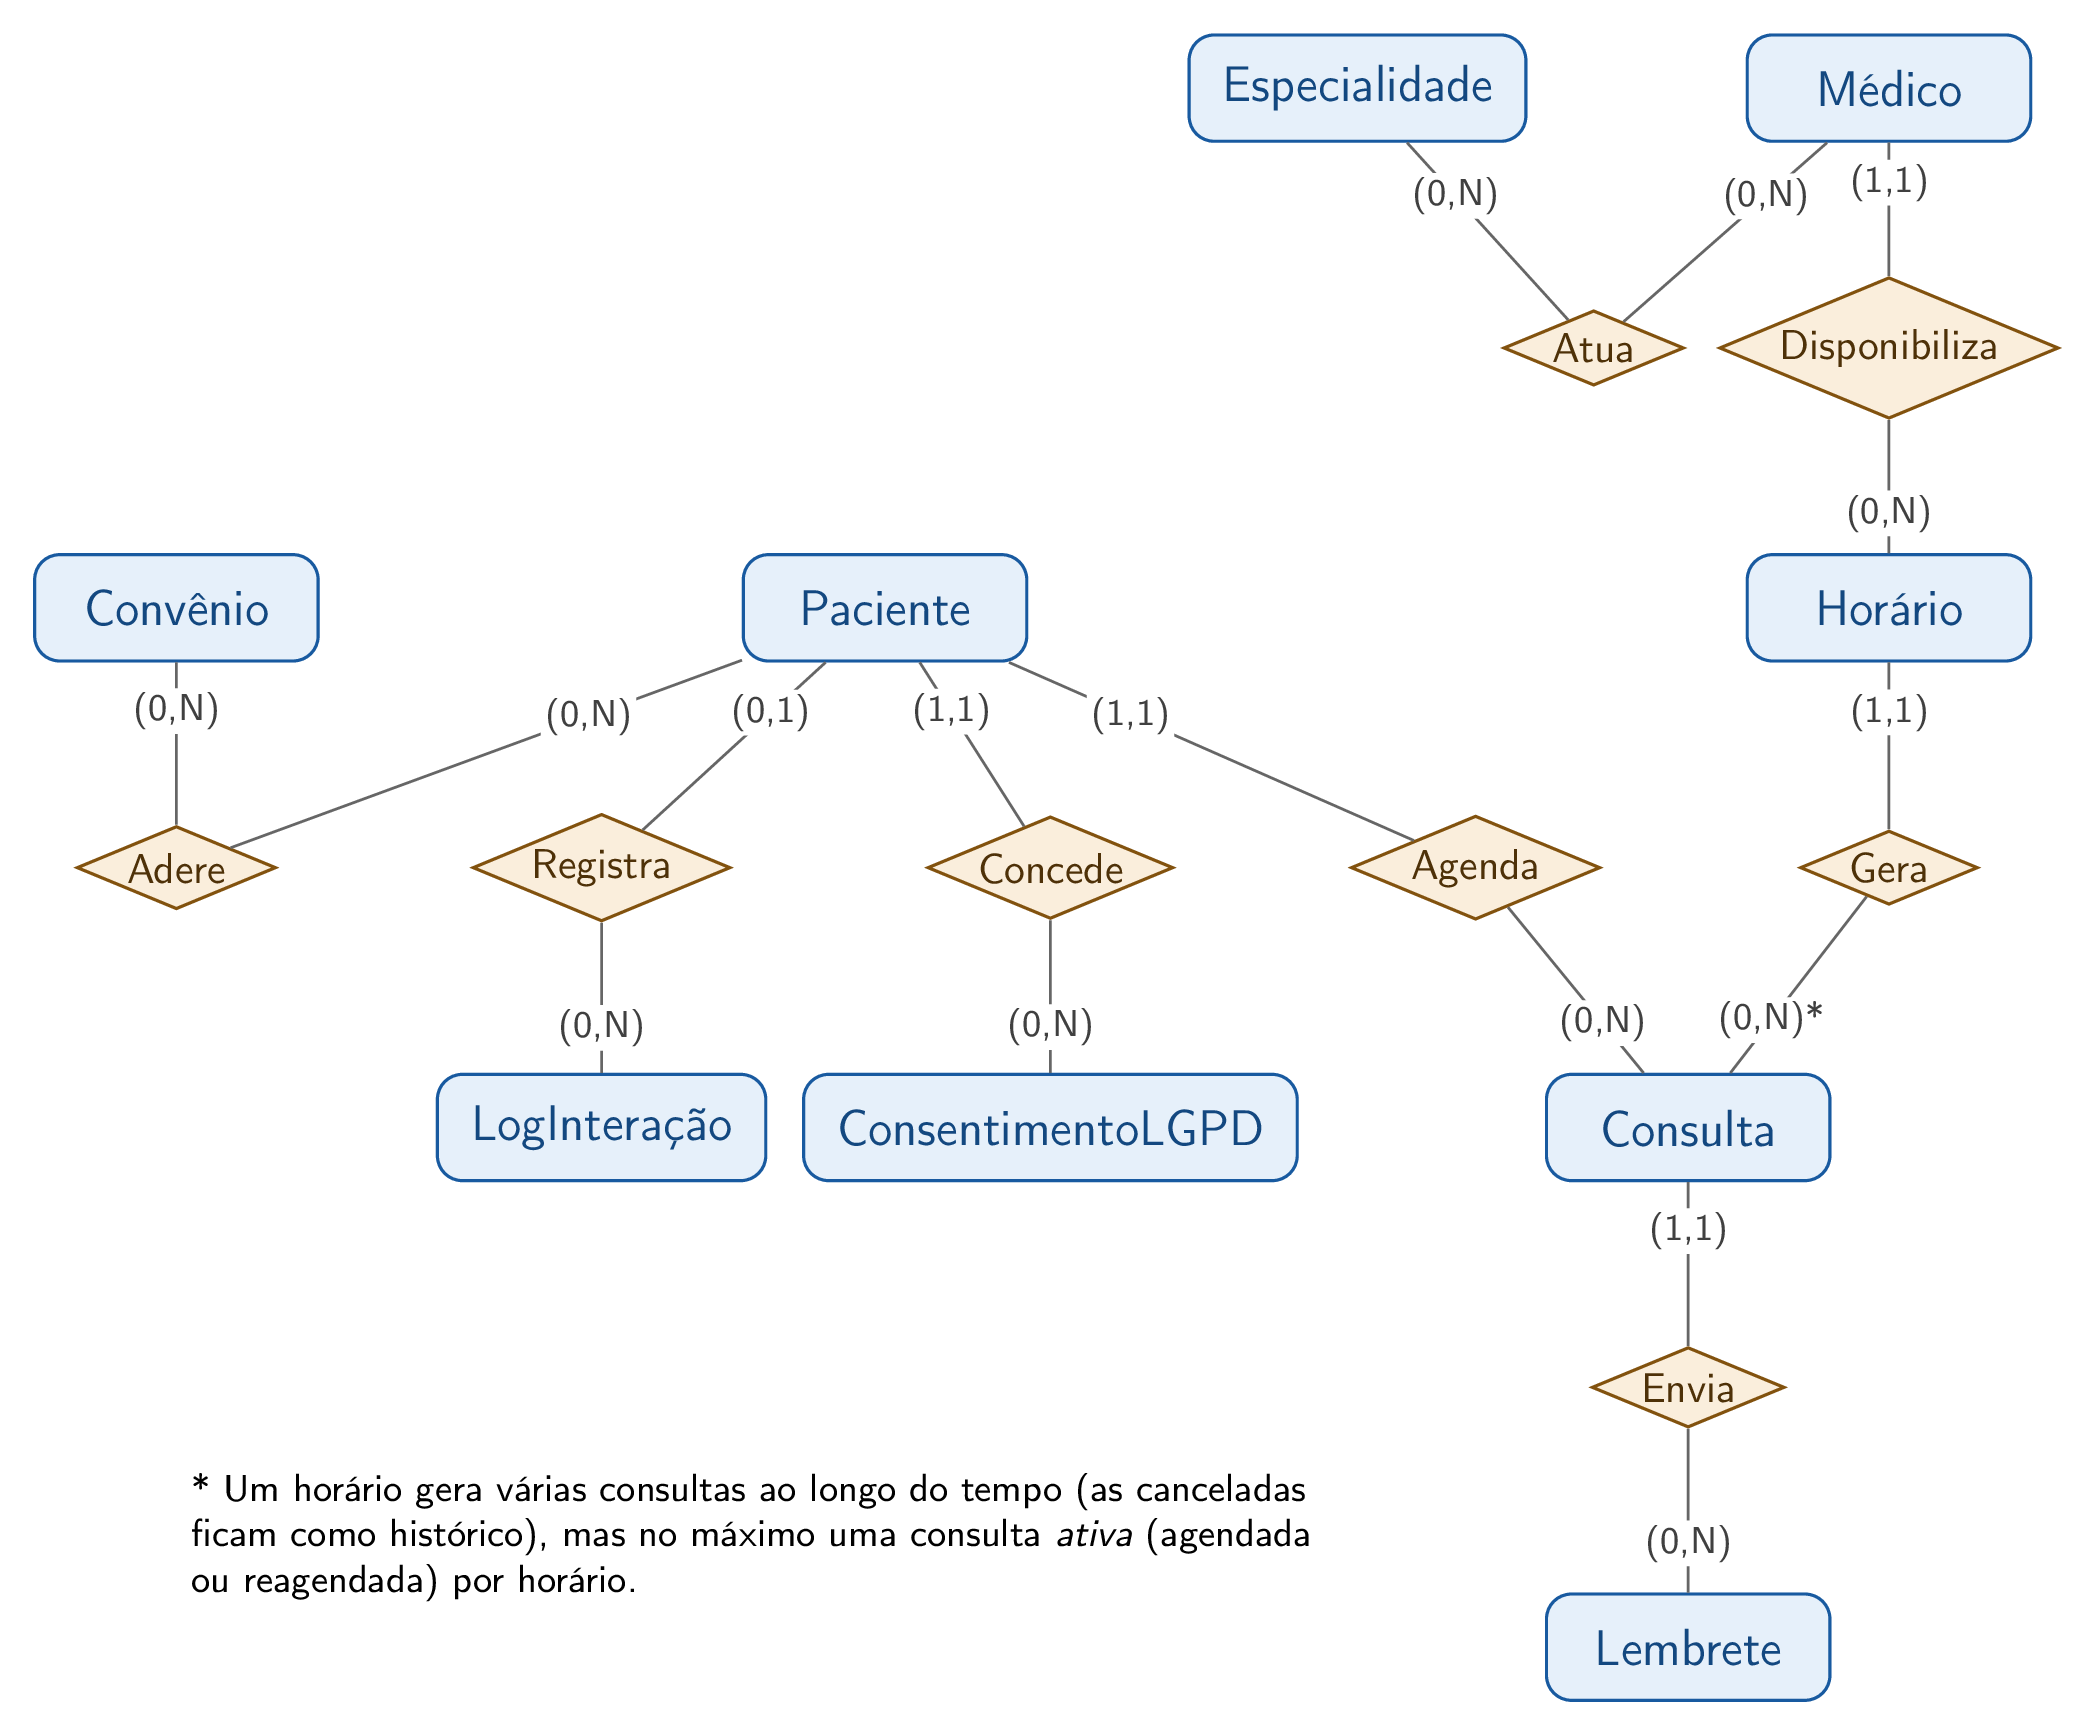
\includegraphics[width=1.0\textwidth]{MERConceitual.png}
    \label{fig:mer-conceitual}
    \vspace{0.2cm}
    \footnotesize{Fonte: Elaborado pelo autor (2026), com base em Heuser (2009) e Bender e Sartipi (2013).}
\end{figure}

\subsubsection{Modelo Lógico}

O modelo lógico traduz o MER da seção 4.4.1 para o modelo relacional, definindo chaves primárias (PK), chaves estrangeiras (FK) e restrições de domínio para cada tabela, em conformidade com os princípios de normalização até a terceira forma normal (3FN) discutidos por Elmasri e Navathe (2016) e Silberschatz, Korth e Sudarshan (2020). A Figura \ref{fig:modelo-logico} apresenta o modelo lógico completo, já com os atributos de cada tabela.

\begin{figure}[H]
    \centering
    \caption{Modelo lógico do banco de dados do protótipo}
    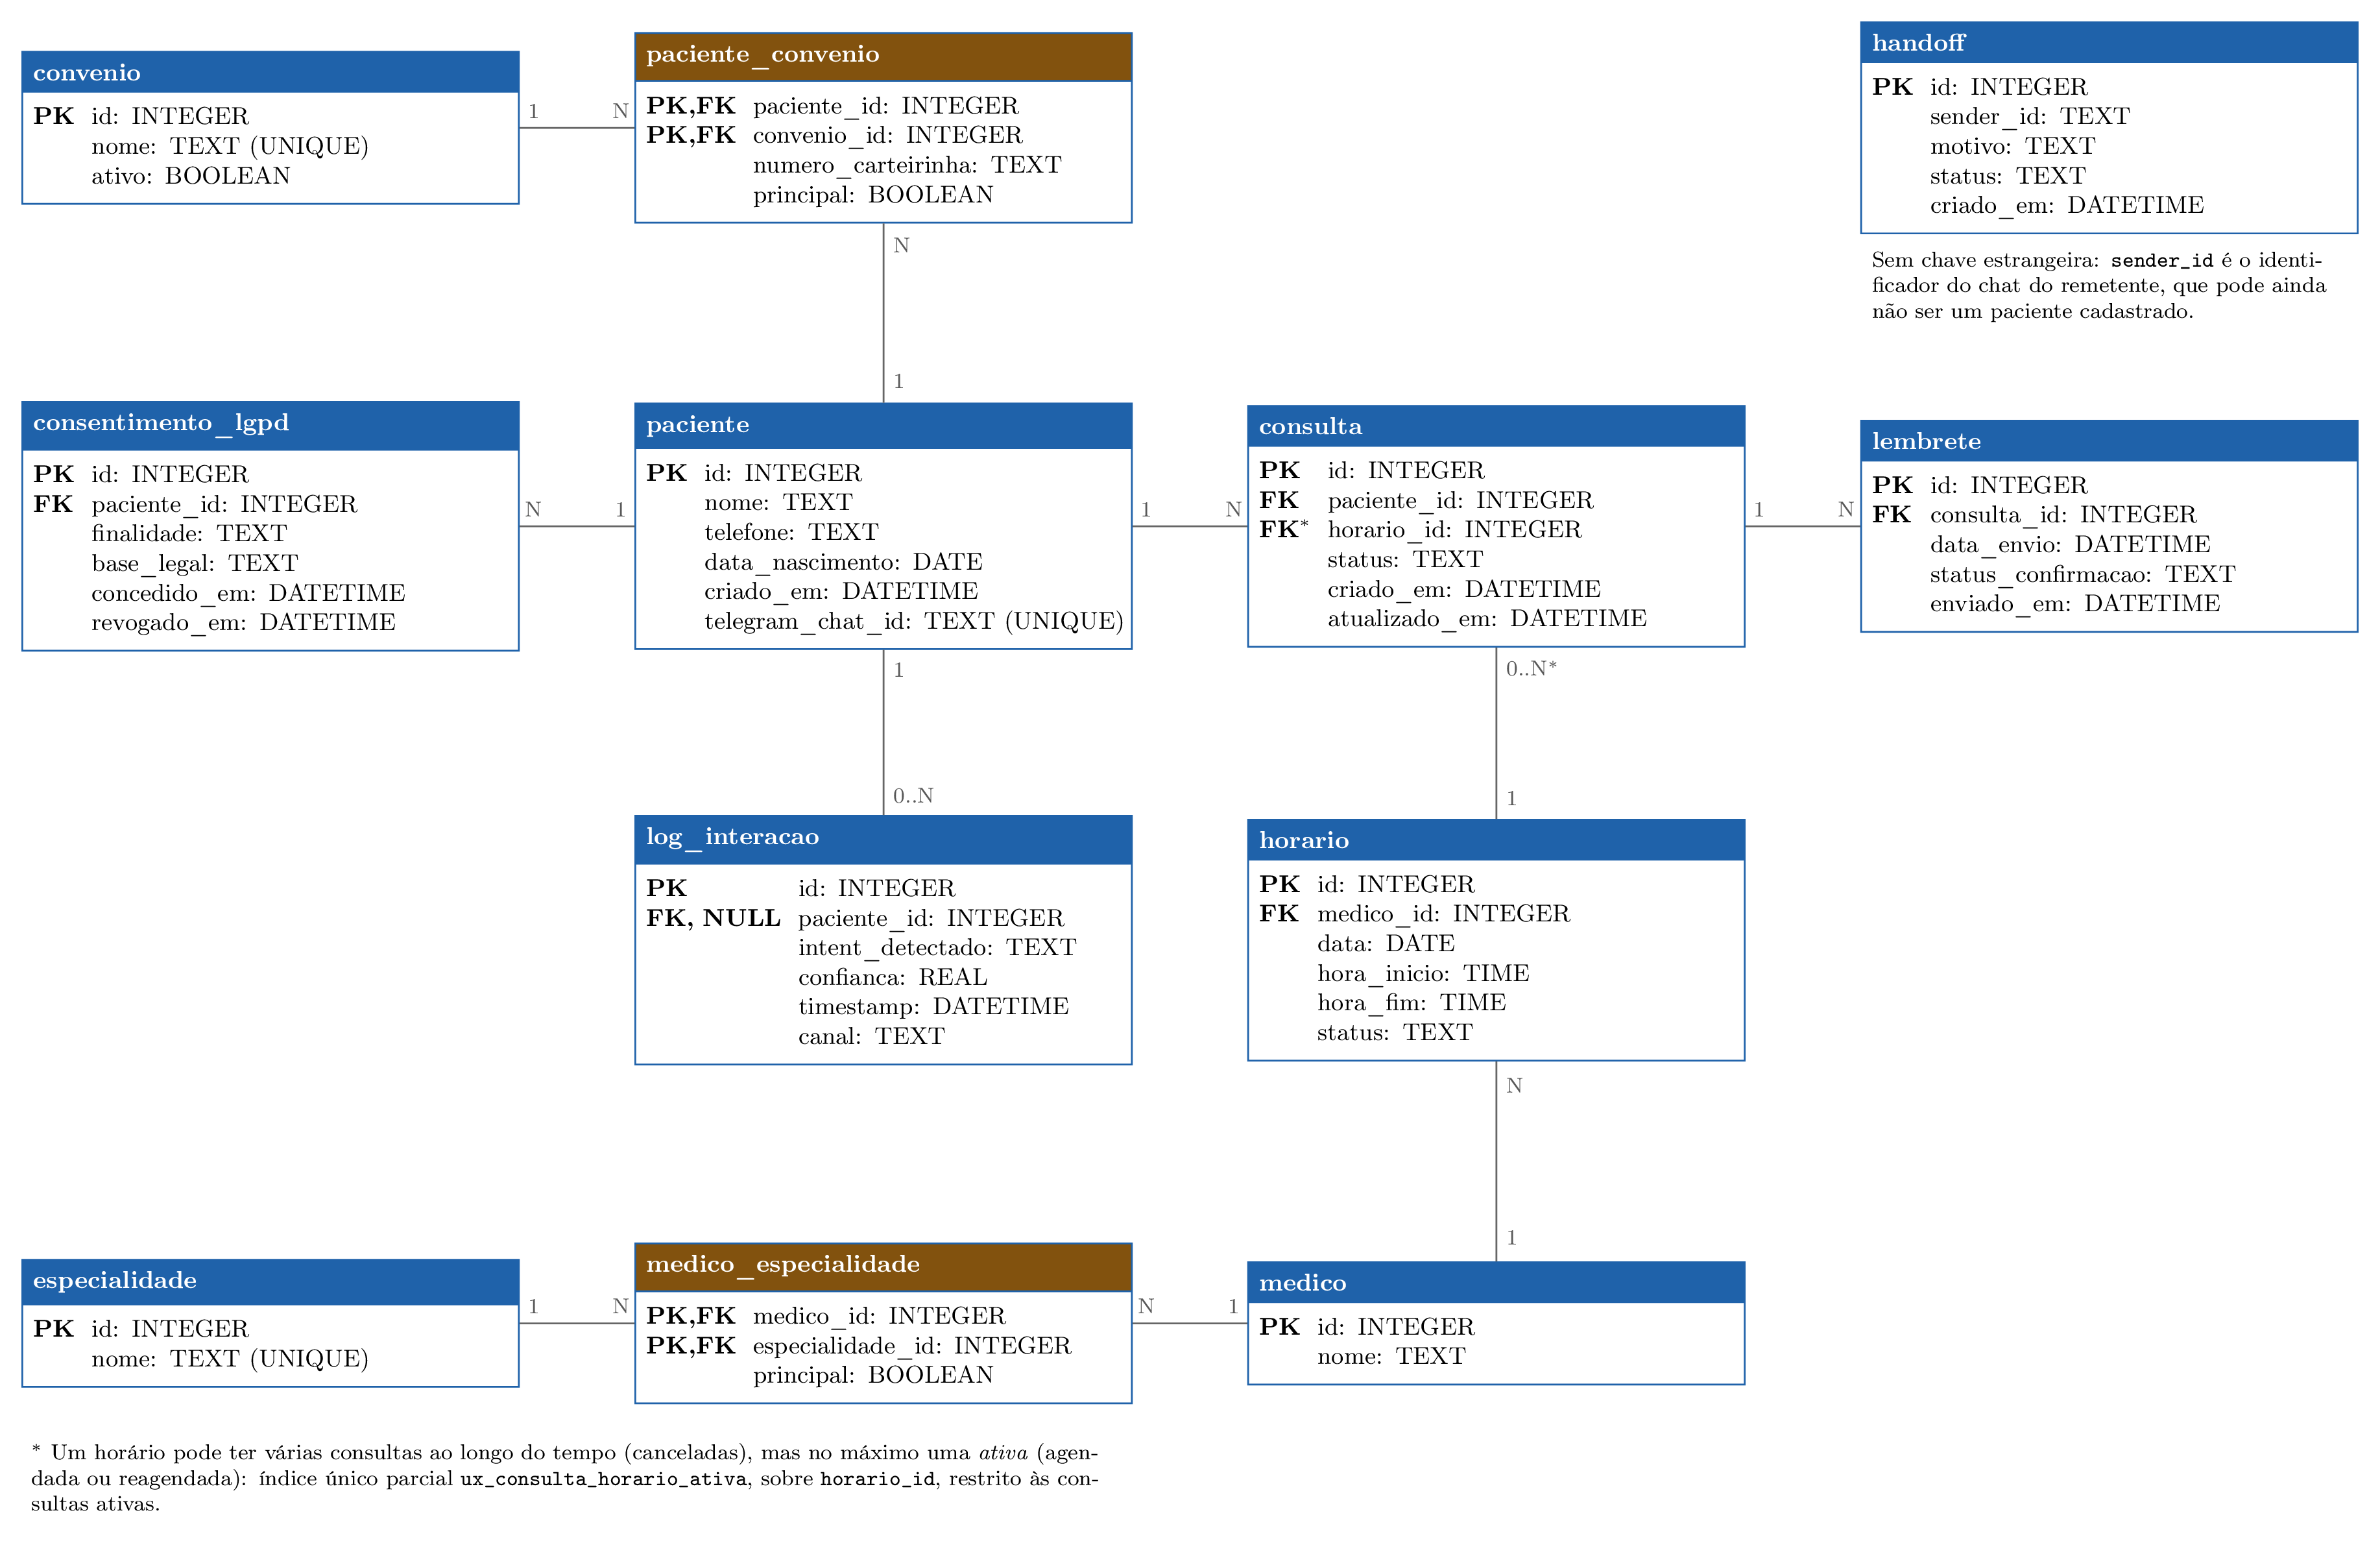
\includegraphics[angle=90,width=\textwidth,height=0.82\textheight,keepaspectratio]{fig_modelo_logico.png}\par
    \label{fig:modelo-logico}
    \vspace{0.2cm}
    \footnotesize{Fonte: Elaborado pelo autor (2026), com base em Elmasri e Navathe (2016).}
\end{figure}

As tabelas e suas chaves são apresentadas na Tabela \ref{tab:chaves-tabelas}.

\begin{table}[H]
    \centering
    \caption{Tabelas do modelo lógico e suas chaves}
    \label{tab:chaves-tabelas}

    \small
    \setlength{\tabcolsep}{4pt}

    \begin{tabularx}{\textwidth}{
        >{\raggedright\arraybackslash}p{0.23\textwidth}
        >{\raggedright\arraybackslash}p{0.25\textwidth}
        >{\raggedright\arraybackslash}X
    }
        \hline
        \textbf{Tabela} &
        \textbf{Chave primária (PK)} &
        \textbf{Chaves estrangeiras (FK)} \\
        \hline

        convenio
        & id
        & --- \\
        \hline

        especialidade
        & id
        & --- \\
        \hline

        medico
        & id
        & --- \\
        \hline

        medico\_\allowbreak{}especialidade
        & (medico\_\allowbreak{}id, especialidade\_\allowbreak{}id)
        & medico\_\allowbreak{}id $\rightarrow$ medico(id);
          especialidade\_\allowbreak{}id $\rightarrow$ especialidade(id) \\
        \hline

        paciente
        & id
        & --- \\
        \hline

        paciente\_\allowbreak{}convenio
        & (paciente\_\allowbreak{}id, convenio\_\allowbreak{}id)
        & paciente\_\allowbreak{}id $\rightarrow$ paciente(id);
          convenio\_\allowbreak{}id $\rightarrow$ convenio(id) \\
        \hline

        horario
        & id
        & medico\_\allowbreak{}id $\rightarrow$ medico(id) \\
        \hline

        consulta
        & id
        & paciente\_\allowbreak{}id $\rightarrow$ paciente(id);
          horario\_\allowbreak{}id $\rightarrow$ horario(id),
          \textbf{índice único parcial} \\
        \hline

        consentimento\_\allowbreak{}lgpd
        & id
        & paciente\_\allowbreak{}id $\rightarrow$ paciente(id) \\
        \hline

        log\_\allowbreak{}interacao
        & id
        & paciente\_\allowbreak{}id $\rightarrow$ paciente(id), nullable \\
        \hline

        lembrete
        & id
        & consulta\_\allowbreak{}id $\rightarrow$ consulta(id) \\
        \hline

        handoff
        & id
        & --- (guarda o \texttt{sender\_\allowbreak{}id}, chat do remetente) \\
        \hline

    \end{tabularx}

    \vspace{0.1cm}

    \footnotesize
    Fonte: Elaborado pelo autor, 2026.
\end{table}

Três decisões de projeto merecem destaque nesta etapa. Primeiro, um índice único parcial sobre \texttt{consulta.horario\_\allowbreak{}id}, restrito às consultas com situação \texttt{agendada} ou \texttt{reagendada}, implementa em nível de banco de dados a regra de no máximo uma consulta ativa por horário, impedindo o duplo agendamento sem impedir que um horário liberado por cancelamento seja reservado novamente e preservando o histórico das consultas canceladas. Segundo, a coluna \texttt{paciente\_\allowbreak{}id} da tabela \texttt{log\_\allowbreak{}interacao} foi definida como opcional (\textit{nullable}), refletindo o fato de que o classificador de intenção pode processar uma mensagem antes de o sistema identificar o paciente correspondente, situação comum no início de uma conversa. Terceiro, as tabelas \texttt{medico\_\allowbreak{}especialidade} e \texttt{paciente\_\allowbreak{}convenio} adotam chave primária composta, prática recomendada por Elmasri e Navathe (2016) para entidades associativas puras, e incluem uma coluna booleana \texttt{principal}, que resolve o critério de desempate quando um médico possui mais de uma especialidade ou um paciente mais de um convênio. Essa decisão tem precedente direto no padrão HL7 FHIR adotado na camada de integração do sistema (seção 4.1): o recurso \textit{Coverage}, que representa a cobertura de um paciente, define um atributo \texttt{order} para indicar qual cobertura é a primária quando há mais de uma (HL7 INTERNATIONAL, 2024a); e o recurso \textit{PractitionerRole} permite repetir o elemento \texttt{specialty} quando o mesmo profissional atua em mais de uma especialidade (HL7 INTERNATIONAL, 2024b). O esquema físico completo, incluindo tipos de dados, restrições de checagem (\texttt{CHECK}) e índices de desempenho, está detalhado no Apêndice~\ref{ap:ddl} (script DDL). Duas alterações foram incorporadas ao modelo durante a implementação. A primeira é a coluna \texttt{telegram\_\allowbreak{}chat\_\allowbreak{}id} na tabela \texttt{paciente}, com restrição de unicidade, que associa o paciente ao seu canal de conversa e substitui o paciente fixo utilizado nos testes iniciais. A segunda é a coluna \texttt{enviado\_\allowbreak{}em} na tabela \texttt{lembrete}, que, ao permanecer nula, indica que o lembrete ainda não foi enviado; sem ela, o modelo original não distinguia um lembrete programado de um lembrete já enviado e aguardando confirmação.

\subsubsection{Dicionário de Dados}

O dicionário de dados descreve, para cada tabela do modelo lógico, o nome, o tipo, as restrições e o significado de cada campo, seguindo o formato recomendado por Heuser (2009) para documentação de esquemas relacionais.

\begin{table}[H]
    \centering
    \caption{Dicionário de dados --- tabela \texttt{convenio}}
    {\small
    \begin{tabularx}{\textwidth}{@{}L{3.3cm} L{1.8cm} L{4.0cm} Y@{}}
        \toprule
        \textbf{Campo} & \textbf{Tipo} & \textbf{Restrição} & \textbf{Descrição} \\
        \midrule
        id & INTEGER & PK, autoincremento & Identificador único do convênio \\
        nome & TEXT & NOT NULL, UNIQUE & Nome do convênio (ex.: ``Unimed'') \\
        ativo & BOOLEAN & NOT NULL, default true & Indica se o convênio ainda é aceito pela clínica \\
        \bottomrule
    \end{tabularx}
    }
    \vspace{0.12cm}
    {\raggedright\footnotesize Fonte: Elaborado pelo autor, 2026.\par}
\end{table}

\begin{table}[H]
    \centering
    \caption{Dicionário de dados --- tabela \texttt{especialidade}}
    {\small
    \begin{tabularx}{\textwidth}{@{}L{3.3cm} L{1.8cm} L{4.0cm} Y@{}}
        \toprule
        \textbf{Campo} & \textbf{Tipo} & \textbf{Restrição} & \textbf{Descrição} \\
        \midrule
        id & INTEGER & PK, autoincremento & Identificador único da especialidade \\
        nome & TEXT & NOT NULL, UNIQUE & Nome da especialidade médica (ex.: ``Cardiologia'') \\
        \bottomrule
    \end{tabularx}
    }
    \vspace{0.12cm}
    {\raggedright\footnotesize Fonte: Elaborado pelo autor, 2026.\par}
\end{table}

\begin{table}[H]
    \centering
    \caption{Dicionário de dados --- tabela \texttt{medico}}
    {\small
    \begin{tabularx}{\textwidth}{@{}L{3.3cm} L{1.8cm} L{4.0cm} Y@{}}
        \toprule
        \textbf{Campo} & \textbf{Tipo} & \textbf{Restrição} & \textbf{Descrição} \\
        \midrule
        id & INTEGER & PK, autoincremento & Identificador único do médico \\
        nome & TEXT & NOT NULL & Nome completo do médico \\
        \bottomrule
    \end{tabularx}
    }
    \vspace{0.12cm}
    {\raggedright\footnotesize Fonte: Elaborado pelo autor, 2026.\par}
\end{table}

\begin{table}[H]
    \centering
    \caption{Dicionário de dados --- tabela \texttt{medico\_\allowbreak{}especialidade}}
    {\small
    \begin{tabularx}{\textwidth}{@{}L{3.3cm} L{1.8cm} L{4.0cm} Y@{}}
        \toprule
        \textbf{Campo} & \textbf{Tipo} & \textbf{Restrição} & \textbf{Descrição} \\
        \midrule
        medico\_\allowbreak{}id & INTEGER & PK (composta), FK $\rightarrow$ medico(id) & Médico vinculado à especialidade \\
        especialidade\_\allowbreak{}id & INTEGER & PK (composta), FK $\rightarrow$ especialidade(id) & Especialidade exercida pelo médico \\
        principal & BOOLEAN & NOT NULL, default false & Indica a especialidade principal do médico, usada como critério de desempate em buscas por especialidade (RF02, RF03) \\
        \bottomrule
    \end{tabularx}
    }
    \vspace{0.12cm}
    {\raggedright\footnotesize Fonte: Elaborado pelo autor, 2026.\par}
\end{table}

\begin{table}[H]
    \centering
    \caption{Dicionário de dados --- tabela \texttt{paciente}}
    {\small
    \begin{tabularx}{\textwidth}{@{}L{3.3cm} L{1.8cm} L{4.0cm} Y@{}}
        \toprule
        \textbf{Campo} & \textbf{Tipo} & \textbf{Restrição} & \textbf{Descrição} \\
        \midrule
        id & INTEGER & PK, autoincremento & Identificador único do paciente \\
        nome & TEXT & NOT NULL & Nome completo do paciente \\
        telefone & TEXT & NOT NULL & Telefone de contato informado no cadastro (somente dígitos, com DDD) \\
        data\_\allowbreak{}nascimento & DATE & NOT NULL & Data de nascimento do paciente \\
        criado\_\allowbreak{}em & DATETIME & NOT NULL, default now & Data e hora do cadastro do paciente \\
        telegram\_\allowbreak{}chat\_\allowbreak{}id & TEXT & UNIQUE, nullable & Identificador do chat do Telegram; identifica o paciente na conversa e é o destino dos lembretes (RF08, RF10) \\
        \bottomrule
    \end{tabularx}
    }
    \vspace{0.12cm}
    {\raggedright\footnotesize Fonte: Elaborado pelo autor, 2026.\par}
\end{table}

\begin{table}[H]
    \centering
    \caption{Dicionário de dados --- tabela \texttt{paciente\_\allowbreak{}convenio}}
    {\small
    \begin{tabularx}{\textwidth}{@{}L{3.3cm} L{1.8cm} L{4.0cm} Y@{}}
        \toprule
        \textbf{Campo} & \textbf{Tipo} & \textbf{Restrição} & \textbf{Descrição} \\
        \midrule
        paciente\_\allowbreak{}id & INTEGER & PK (composta), FK $\rightarrow$ paciente(id) & Paciente titular do convênio \\
        convenio\_\allowbreak{}id & INTEGER & PK (composta), FK $\rightarrow$ convenio(id) & Convênio ao qual o paciente aderiu \\
        numero\_\allowbreak{}carteirinha & TEXT & nullable & Número da carteirinha do convênio \\
        principal & BOOLEAN & NOT NULL, default false & Indica o convênio prioritário para faturamento, análogo ao atributo \texttt{order} do recurso \textit{Coverage} da HL7 FHIR \\
        \bottomrule
    \end{tabularx}
    }
    \vspace{0.12cm}
    {\raggedright\footnotesize Fonte: Elaborado pelo autor, 2026.\par}
\end{table}

\begin{table}[H]
    \centering
    \caption{Dicionário de dados --- tabela \texttt{horario}}
    {\small
    \begin{tabularx}{\textwidth}{@{}L{3.3cm} L{1.8cm} L{4.0cm} Y@{}}
        \toprule
        \textbf{Campo} & \textbf{Tipo} & \textbf{Restrição} & \textbf{Descrição} \\
        \midrule
        id & INTEGER & PK, autoincremento & Identificador único do horário (\textit{Slot} FHIR) \\
        medico\_\allowbreak{}id & INTEGER & FK $\rightarrow$ medico(id), NOT NULL & Médico ao qual o horário pertence \\
        data & DATE & NOT NULL & Data do horário \\
        hora\_\allowbreak{}inicio & TIME & NOT NULL & Horário de início da janela de atendimento \\
        hora\_\allowbreak{}fim & TIME & NOT NULL & Horário de término da janela de atendimento \\
        status & TEXT & NOT NULL, CHECK IN (disponivel, reservado, bloqueado) & Situação atual do horário \\
        \bottomrule
    \end{tabularx}
    }
    \vspace{0.12cm}
    {\raggedright\footnotesize Fonte: Elaborado pelo autor, 2026.\par}
\end{table}

\begin{table}[H]
    \centering
    \caption{Dicionário de dados --- tabela \texttt{consulta}}
    {\small
    \begin{tabularx}{\textwidth}{@{}L{3.3cm} L{1.8cm} L{4.0cm} Y@{}}
        \toprule
        \textbf{Campo} & \textbf{Tipo} & \textbf{Restrição} & \textbf{Descrição} \\
        \midrule
        id & INTEGER & PK, autoincremento & Identificador único da consulta (\textit{Appointment} FHIR) \\
        paciente\_\allowbreak{}id & INTEGER & FK $\rightarrow$ paciente(id), NOT NULL & Paciente que agendou a consulta \\
        horario\_\allowbreak{}id & INTEGER & FK $\rightarrow$ horario(id), NOT NULL; índice único parcial (consultas ativas) & Horário reservado para a consulta \\
        status & TEXT & NOT NULL, CHECK IN (agendada, cancelada, reagendada, concluida) & Situação atual da consulta \\
        criado\_\allowbreak{}em & DATETIME & NOT NULL, default now & Data e hora do registro da consulta \\
        atualizado\_\allowbreak{}em & DATETIME & NOT NULL, default now & Data e hora da última atualização de status \\
        \bottomrule
    \end{tabularx}
    }
    \vspace{0.12cm}
    {\raggedright\footnotesize Fonte: Elaborado pelo autor, 2026.\par}
\end{table}

\begin{table}[H]
    \centering
    \caption{Dicionário de dados --- tabela \texttt{lembrete}}
    {\small
    \begin{tabularx}{\textwidth}{@{}L{3.3cm} L{1.8cm} L{4.0cm} Y@{}}
        \toprule
        \textbf{Campo} & \textbf{Tipo} & \textbf{Restrição} & \textbf{Descrição} \\
        \midrule
        id & INTEGER & PK, autoincremento & Identificador único do lembrete \\
        consulta\_\allowbreak{}id & INTEGER & FK $\rightarrow$ consulta(id), NOT NULL & Consulta à qual o lembrete se refere \\
        data\_\allowbreak{}envio & DATETIME & NOT NULL & Data e hora programadas para o envio do lembrete, 24 horas antes da consulta (RF08) \\
        status\_\allowbreak{}confirmacao & TEXT & NOT NULL, CHECK IN (pendente, confirmado, ignorado), default pendente & Situação da confirmação de presença pelo paciente (RF09); ``ignorado'' também indica lembrete cancelado ou não enviado \\
        enviado\_\allowbreak{}em & DATETIME & nullable & Data e hora em que o lembrete foi efetivamente enviado; nulo enquanto não enviado \\
        \bottomrule
    \end{tabularx}
    }
    \vspace{0.12cm}
    {\raggedright\footnotesize Fonte: Elaborado pelo autor, 2026.\par}
\end{table}

\begin{table}[H]
    \centering
    \caption{Dicionário de dados --- tabela \texttt{consentimento\_\allowbreak{}lgpd}}
    {\small
    \begin{tabularx}{\textwidth}{@{}L{3.3cm} L{1.8cm} L{4.0cm} Y@{}}
        \toprule
        \textbf{Campo} & \textbf{Tipo} & \textbf{Restrição} & \textbf{Descrição} \\
        \midrule
        id & INTEGER & PK, autoincremento & Identificador único do registro de consentimento \\
        paciente\_\allowbreak{}id & INTEGER & FK $\rightarrow$ paciente(id), NOT NULL & Paciente titular do consentimento \\
        finalidade & TEXT & NOT NULL & Finalidade específica do tratamento: ``agendamento de consultas e atendimento administrativo'' ou ``envio de lembretes e confirmação de presença'' (art. 8º, §4º, LGPD) \\
        base\_\allowbreak{}legal & TEXT & NOT NULL & Base legal invocada: consentimento do titular (art. 7º, I, e art. 11, I, LGPD) \\
        concedido\_\allowbreak{}em & DATETIME & NOT NULL, default now & Data e hora do aceite pelo paciente \\
        revogado\_\allowbreak{}em & DATETIME & nullable & Data e hora da revogação; nulo enquanto o consentimento estiver vigente \\
        \bottomrule
    \end{tabularx}
    }
    \vspace{0.12cm}
    {\raggedright\footnotesize Fonte: Elaborado pelo autor, 2026.\par}
\end{table}

\begin{table}[H]
    \centering
    \caption{Dicionário de dados --- tabela \texttt{log\_\allowbreak{}interacao}}
    {\small
    \begin{tabularx}{\textwidth}{@{}L{3.3cm} L{1.8cm} L{4.0cm} Y@{}}
        \toprule
        \textbf{Campo} & \textbf{Tipo} & \textbf{Restrição} & \textbf{Descrição} \\
        \midrule
        id & INTEGER & PK, autoincremento & Identificador único do registro de log \\
        paciente\_\allowbreak{}id & INTEGER & FK $\rightarrow$ paciente(id), nullable & Paciente associado à interação, se identificado \\
        intent\_\allowbreak{}detectado & TEXT & NOT NULL & Intenção classificada pelo módulo de PLN (RF01) \\
        confianca & REAL & NOT NULL & Score de confiança da classificação (0,0 a 1,0) \\
        timestamp & DATETIME & NOT NULL, default now & Data e hora da interação \\
        canal & TEXT & NOT NULL, default ``chatbot'' & Canal pelo qual a interação ocorreu \\
        \bottomrule
    \end{tabularx}
    }
    \vspace{0.12cm}
    {\raggedright\footnotesize Fonte: Elaborado pelo autor, 2026.\par}
\end{table}

\begin{table}[H]
    \centering
    \caption{Dicionário de dados --- tabela \texttt{handoff}}
    {\small
    \begin{tabularx}{\textwidth}{@{}L{3.3cm} L{1.8cm} L{4.0cm} Y@{}}
        \toprule
        \textbf{Campo} & \textbf{Tipo} & \textbf{Restrição} & \textbf{Descrição} \\
        \midrule
        id & INTEGER & PK, autoincremento & Identificador único do chamado \\
        sender\_\allowbreak{}id & TEXT & NOT NULL & Identificador do chat do remetente no canal (no Telegram, o \textit{chat\_id}); pode ainda não corresponder a um paciente cadastrado \\
        motivo & TEXT & opcional & Motivo do encaminhamento (ex.: baixa confiança do NLU, pedido de atendente) \\
        status & TEXT & NOT NULL, CHECK (aguardando, em\_\allowbreak{}atendimento, encerrado), default ``aguardando'' & Situação do chamado de atendimento humano \\
        criado\_\allowbreak{}em & DATETIME & NOT NULL, default now & Data e hora de abertura do chamado \\
        \bottomrule
    \end{tabularx}
    }
    \vspace{0.12cm}
    {\raggedright\footnotesize Fonte: Elaborado pelo autor, 2026.\par}
\end{table}

\subsection{Prototipação da Interface}
\label{sec:interface}

A interface do protótipo é a própria conversa no Telegram, e não uma tela desenvolvida para o sistema. Por isso, a prototipação consistiu em projetar o fluxo das mensagens: os diagramas de atividades (seção~\ref{sec:modelagem-uml}) definiram a ordem das perguntas e as decisões, e o texto de cada mensagem foi escrito no domínio do Rasa e nas ações customizadas. Algumas decisões de interface valem para todos os fluxos: o consentimento é apresentado antes de qualquer pergunta sobre dados pessoais; as opções de horário são numeradas, e o paciente pode responder pelo número, pelo horário ou pelo nome do médico; nenhum registro é gravado sem uma pergunta de confirmação explícita; e o paciente pode digitar ``cancelar'' para interromper o cadastro a qualquer momento.

As Figuras~\ref{fig:conversa-cadastro}, \ref{fig:conversa-agendamento} e~\ref{fig:conversa-remarcacao} reproduzem uma conversa realizada com o protótipo em funcionamento, por um paciente fictício criado pelo autor no banco de dados de teste. As mensagens do chatbot são transcritas sem alteração; apenas a aparência das telas foi redesenhada para impressão.

\begin{figure}[H]
\centering
\caption{Tela de conversa: saudação, consentimento e cadastro}
\label{fig:conversa-cadastro}
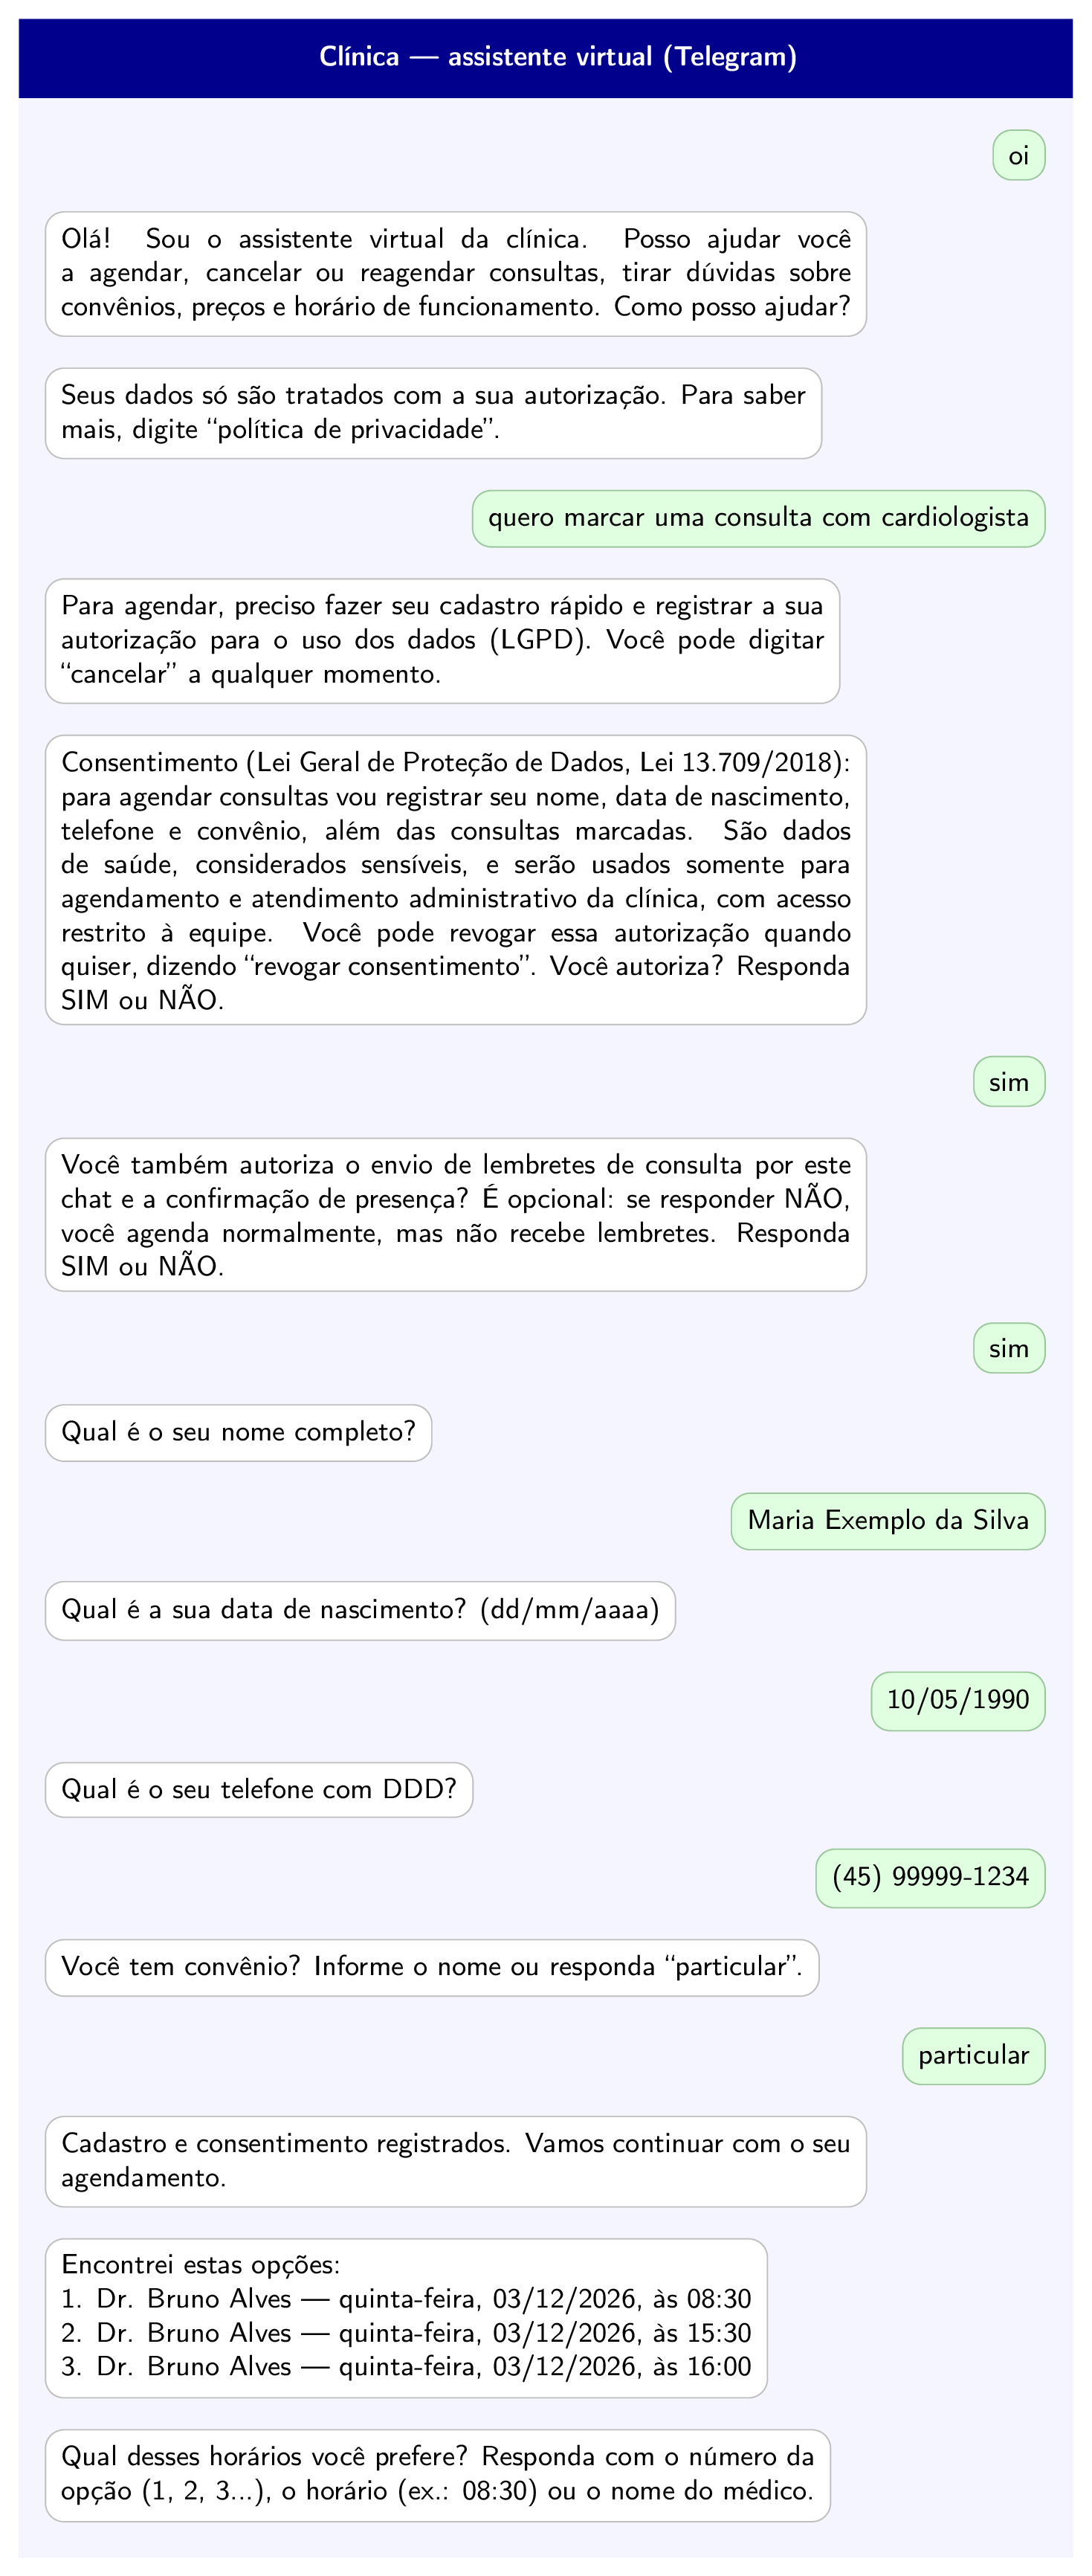
\includegraphics[height=0.78\textheight,keepaspectratio]{fig_conversa_cadastro.png}\par
\vspace{0.2cm}
\footnotesize{Fonte: Elaborado pelo autor, 2026, a partir de conversa com o protótipo (paciente fictício, banco de dados de teste).}
\end{figure}

\begin{figure}[H]
\centering
\caption{Tela de conversa: escolha do horário, confirmação, convênio e consulta do agendamento}
\label{fig:conversa-agendamento}
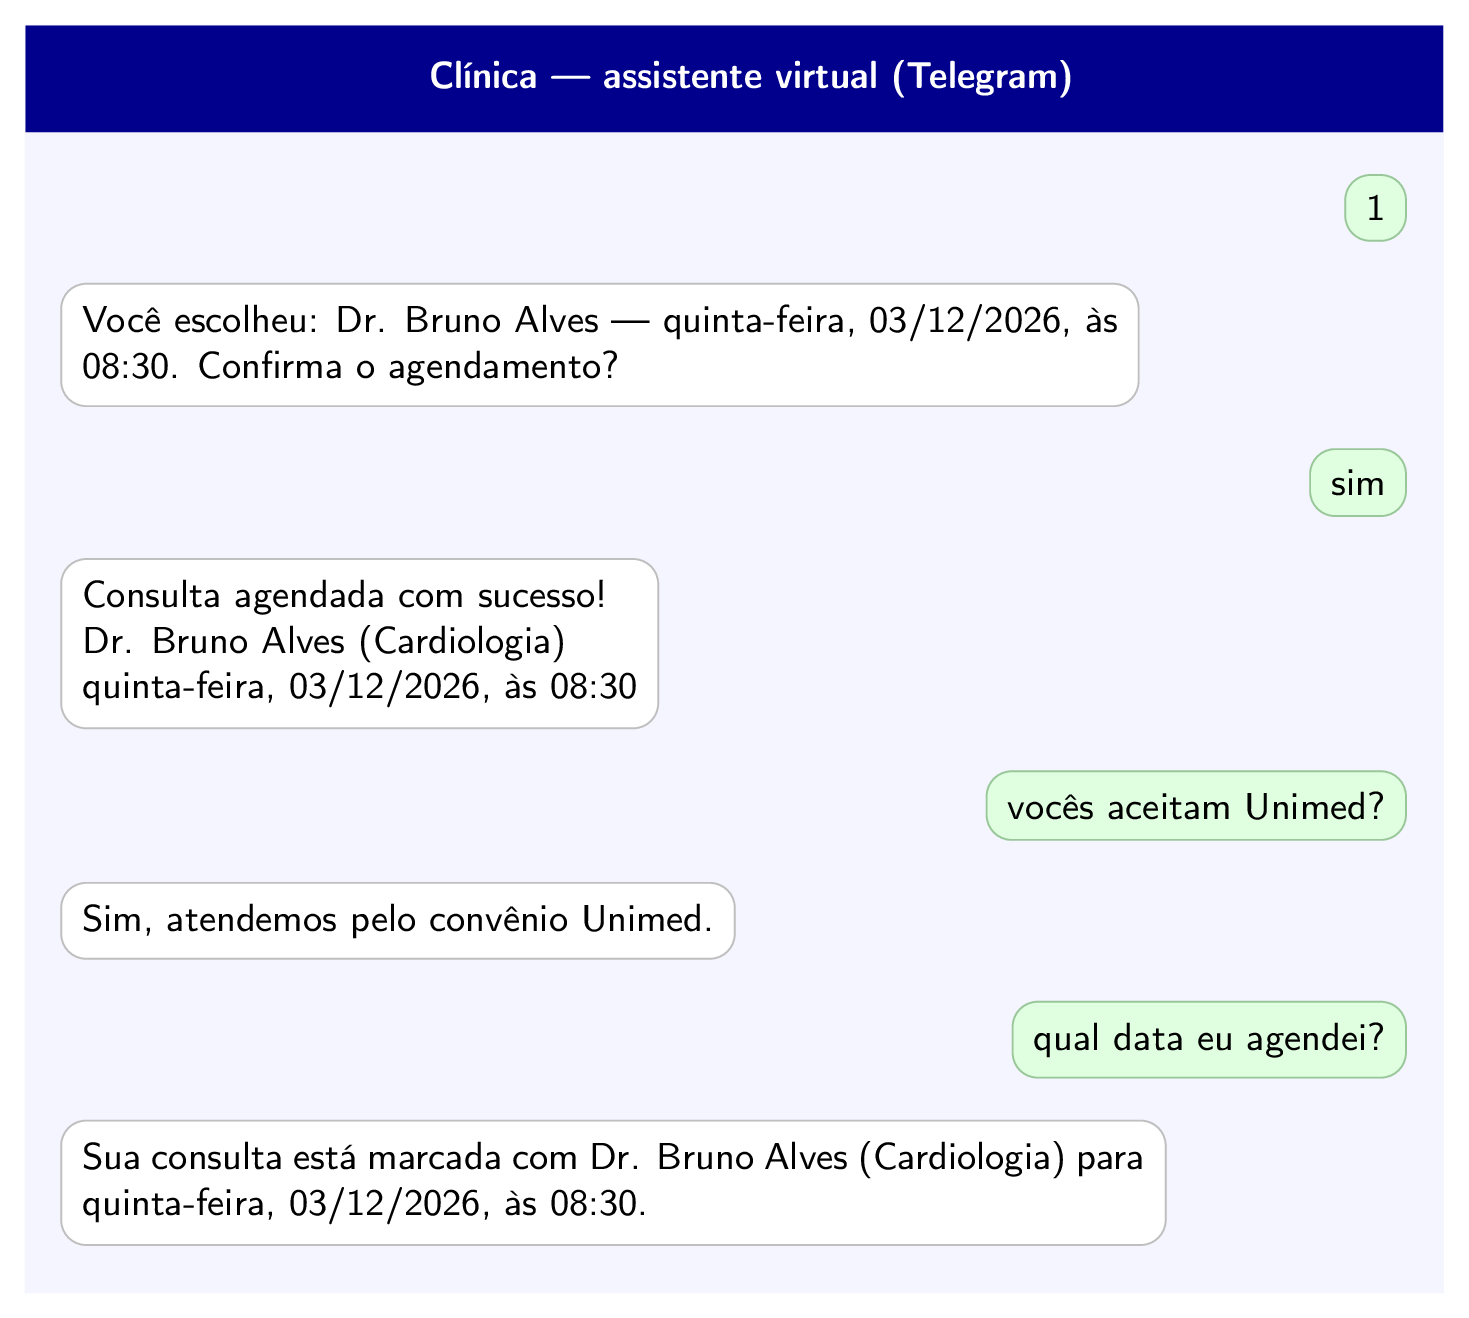
\includegraphics[width=0.75\textwidth]{fig_conversa_agendamento.png}\par
\vspace{0.2cm}
\footnotesize{Fonte: Elaborado pelo autor, 2026, a partir de conversa com o protótipo (paciente fictício, banco de dados de teste).}
\end{figure}

\begin{figure}[H]
\centering
\caption{Tela de conversa: reagendamento e cancelamento}
\label{fig:conversa-remarcacao}
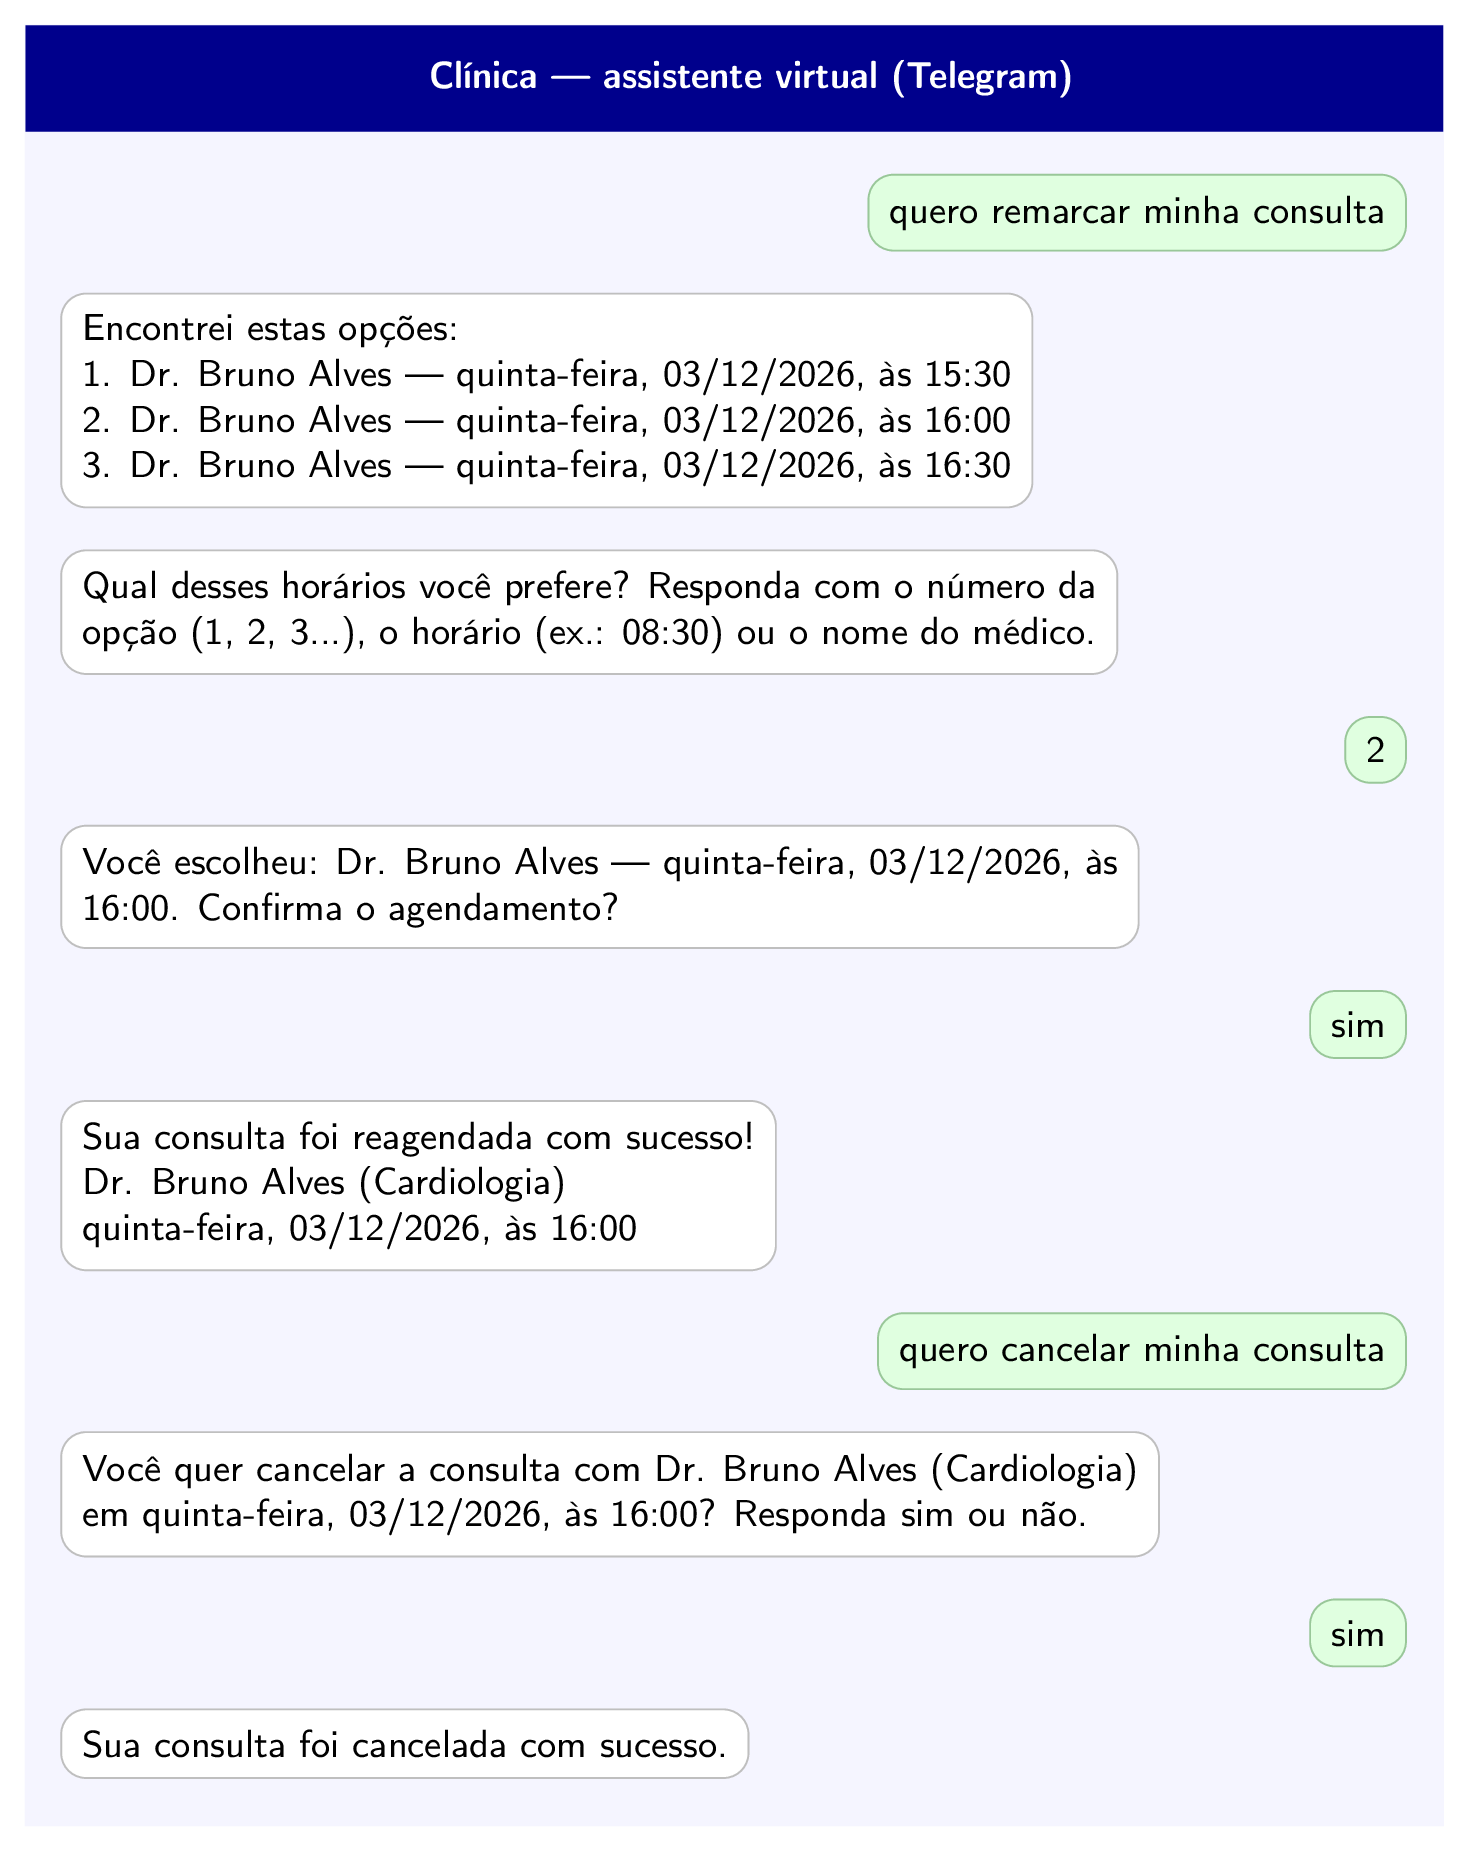
\includegraphics[width=0.75\textwidth]{fig_conversa_remarcacao.png}\par
\vspace{0.2cm}
\footnotesize{Fonte: Elaborado pelo autor, 2026, a partir de conversa com o protótipo (paciente fictício, banco de dados de teste).}
\end{figure}

\subsection{Implementação do Sistema}
\label{sec:implementacao}

Esta seção descreve como o projeto apresentado foi implementado: a organização dos módulos, as funcionalidades implementadas e a integração entre os componentes. O código-fonte, os dados de teste e os resultados de cada execução estão disponíveis no repositório público do trabalho (\url{https://github.com/Jiibara/TCC}).

\subsubsection{Estrutura dos módulos}

O protótipo segue a organização de um projeto Rasa, com o código próprio concentrado no servidor de ações e no canal do Telegram. A Tabela~\ref{tab:modulos} descreve os principais arquivos.

\begin{xltabular}{\textwidth}{p{5.2cm}Y}
\caption{Estrutura dos módulos do protótipo}
\label{tab:modulos}\\
\hline
\textbf{Arquivo} & \textbf{Função} \\
\hline
\endfirsthead
\multicolumn{2}{l}{\small Tabela~\thetable\ (continuação)} \\
\hline
\textbf{Arquivo} & \textbf{Função} \\
\hline
\endhead
\hline
\endfoot
\hline
\endlastfoot
\texttt{rasa/config.yml} & \textit{Pipeline} de NLU (BERTimbau e \texttt{DIETClassifier}), limiares de \textit{fallback} e política de diálogo (\texttt{RulePolicy}) \\
\texttt{rasa/data/nlu.yml} & Corpus de treinamento: 703 frases em 21 intenções, com as entidades anotadas \\
\texttt{rasa/data/rules.yml} & Regras que associam cada intenção, no contexto da conversa, à ação a executar \\
\texttt{rasa/domain.yml} & Intenções, entidades, \textit{slots} (memória da conversa), formulários e respostas fixas \\
\texttt{rasa/actions/actions.py} & Servidor de ações: regras de negócio, consentimento, agendamento, cancelamento, reagendamento, lembretes e acesso ao banco \\
\texttt{rasa/telegram\_custom.py} & Canal do Telegram: recebe as mensagens pelo \textit{webhook}, confirma o recebimento e devolve as respostas \\
\texttt{rasa/enviar\_lembretes.py} & Serviço de lembretes, executado a cada minuto, independente da conversa \\
\texttt{rasa/endpoints.yml} e \texttt{credentials.yml} & Endereço do servidor de ações e configuração dos canais (o token do bot fica fora do repositório) \\
\texttt{schema.sql} e \texttt{seed\_horarios.py} & Criação do banco SQLite e geração dos horários livres da agenda simulada \\
\texttt{cenarios/}, \texttt{ablacao/}, \texttt{resultados/} & Testes funcionais automatizados, experimento de ablação e medições, com os resultados de cada execução \\
\end{xltabular}
\vspace{0.3cm}

\footnotesize{Fonte: Elaborado pelo autor, 2026.}

\normalsize
\subsubsection{Funcionalidades implementadas}

Todos os requisitos funcionais da seção~\ref{sec:requisitos} foram implementados. A Tabela~\ref{tab:funcionalidades} relaciona cada requisito ao componente que o implementa e aos cenários de teste que o verificam (Tabela~\ref{tab:funcionais} e Apêndice~\ref{ap:cenarios}).

\begin{xltabular}{\textwidth}{p{1.9cm}Yp{2.2cm}}
\caption{Requisitos funcionais, componentes que os implementam e cenários de teste}
\label{tab:funcionalidades}\\
\hline
\textbf{Requisito} & \textbf{Implementação} & \textbf{Cenários} \\
\hline
\endfirsthead
\multicolumn{3}{l}{\small Tabela~\thetable\ (continuação)} \\
\hline
\textbf{Requisito} & \textbf{Implementação} & \textbf{Cenários} \\
\hline
\endhead
\hline
\endfoot
\hline
\endlastfoot
RF01, RF02 & \textit{Pipeline} de NLU (\texttt{config.yml}, \texttt{nlu.yml}) & 1, 2, 16 \\
RF03 & \texttt{ActionConsultarDisponibilidade} & 1, 22 \\
RF04 & \texttt{ActionSelecionarHorario}, \texttt{ActionConfirmarAgendamento} & 1, 18, 19, 21 \\
RF05 & \texttt{ActionPedirConfirmacaoCancelamento}, \texttt{executar\_cancelamento} & 3, 19, 23, 25 \\
RF06 & \texttt{ActionConfirmarAgendamento} (reagendamento), \texttt{ActionSelecionarConsulta} & 4, 20, 26 \\
RF07 & \texttt{ActionInformarConvenio} & 5 \\
RF08, RF09 & \texttt{registrar\_lembrete}, \texttt{enviar\_lembretes.py}, \texttt{ActionConfirmarPresenca} & 6, 7 \\
RF10 & \texttt{cadastro\_form}, \texttt{ActionFinalizarCadastro}, \texttt{ActionAtualizarCadastro} & 8, 11, 12, 13 \\
RF11 & \texttt{ActionVerificarCadastro}, tabela \texttt{consentimento\_lgpd} & 8, 9, 10 \\
RF12 & \texttt{FallbackClassifier}, \texttt{ActionEncaminharAtendimentoHumano} & 16 \\
RF13 & \texttt{ActionLogInteracao}, tabela \texttt{log\_interacao} & 24 \\
RF14 & \texttt{ActionRevogarConsentimento} & 14 \\
RF15 & Resposta de política de privacidade (\texttt{domain.yml} e \texttt{rules.yml}) & 15 \\
\end{xltabular}
\vspace{0.3cm}

\footnotesize{Fonte: Elaborado pelo autor, 2026.}

\normalsize
\subsubsection{Integração entre componentes}

Os quatro processos do protótipo se comunicam da seguinte forma. O Telegram envia cada mensagem, por HTTPS, ao \textit{webhook} do canal customizado, que confirma o recebimento imediatamente e repassa a mensagem ao servidor do Rasa. O servidor do Rasa aplica o \textit{pipeline} de NLU, identifica a intenção e as entidades, e a \texttt{RulePolicy} escolhe a próxima ação. Quando a ação é customizada, o servidor do Rasa a solicita ao servidor de ações por HTTP, em endereço local (\texttt{endpoints.yml}), enviando o estado da conversa; o servidor de ações executa a regra de negócio, lê ou grava no banco SQLite e devolve as mensagens e as atualizações de \textit{slots}. As respostas voltam ao paciente pela API do Telegram. O serviço de lembretes não participa da conversa: a cada minuto, consulta o banco, envia pela API do Telegram os lembretes devidos e registra o envio, e a resposta do paciente ao lembrete volta pelo mesmo caminho das demais mensagens. Essa separação permite reiniciar ou alterar um componente sem afetar os demais, conforme o RNF07.

\newpage

% ==========================================
% ANÁLISE DE RESULTADOS
% ==========================================
\section{Análise de Resultados}
\label{cap:resultados}

Esta seção apresenta e discute os resultados obtidos na avaliação do protótipo de chatbot desenvolvido, conforme os procedimentos de teste definidos na seção~\ref{sec:testes-metodo}. Inicialmente são descritos os testes aplicados e as ferramentas utilizadas; em seguida, as métricas coletadas e a forma como foram obtidas; por fim, os resultados são apresentados e confrontados com os critérios de aceitação estabelecidos nos objetivos do trabalho (Tabela~\ref{tab:criterios-sucesso}) e nos requisitos funcionais e não funcionais (Tabelas~\ref{tab:requisitos-funcionais} e~\ref{tab:requisitos-nao-funcionais}).

% ------------------------------------------------------------
\subsection{Procedimentos de Teste}
\label{sec:proc_teste}

A validação do protótipo foi conduzida em ambiente simulado, sem a utilização de dados reais de pacientes e sem identificação dos participantes da avaliação de usabilidade, conforme previsto na metodologia. A agenda médica foi representada por um banco de dados SQLite local, populado com 2 médicos, 4 especialidades, 3 convênios e 353 horários fictícios, modelados a partir dos recursos \textit{Schedule}, \textit{Slot} e \textit{Appointment} do padrão HL7 FHIR.

\subsubsection{Tipos de Testes Aplicados}
\label{sec:tipos_testes}

Foram aplicados três tipos de testes, alinhados à seção~\ref{sec:tipos-metodo}:

\begin{itemize}
    \item \textbf{Testes funcionais:} verificam se cada funcionalidade se comporta conforme o esperado, abrangendo os fluxos de agendamento, cancelamento, reagendamento, consulta de convênios, confirmação de lembretes, cadastro com consentimento, atualização cadastral, revogação de consentimento e solicitação da política de privacidade;
    \item \textbf{Testes de integração:} verificam a comunicação entre o canal de mensageria (Telegram), o servidor do Rasa, o servidor de ações, o banco de dados SQLite e o serviço de lembretes;
    \item \textbf{Testes de desempenho:} compreendem a avaliação do módulo de compreensão de linguagem natural (precisão, revocação e F1-score por intenção e por entidade) e a medição do tempo de resposta do chatbot.
\end{itemize}

Complementarmente, a usabilidade foi avaliada por meio do questionário \textit{System Usability Scale} (SUS), aplicado a cinco avaliadores.

\subsubsection{Ferramentas Utilizadas}
\label{sec:ferramentas}

A Tabela~\ref{tab:ferramentas} sintetiza o ambiente e as ferramentas empregadas na execução dos testes.

\begin{table}[H]
\centering
\caption{Ferramentas e ambiente utilizados nos testes}
\label{tab:ferramentas}
\begin{tabular}{p{4.2cm}p{9cm}}
\hline
\textbf{Ferramenta} & \textbf{Finalidade} \\
\hline
Rasa Open Source 3.6.20 & Compreensão de linguagem natural (classificação de intenção e NER) e gerenciamento do diálogo (\textit{rules} e \textit{forms}) \\
Rasa SDK 3.6.2 & Execução das \textit{custom actions} em servidor de ações independente \\
Python 3.8 & Linguagem de implementação das ações, do canal customizado e do serviço de lembretes \\
BERTimbau (\texttt{neuralmind/\allowbreak bert-base-\allowbreak portuguese-cased}) & Modelo de linguagem pré-treinado para o português brasileiro, usado como extrator de características (\texttt{LanguageModel\allowbreak{}Featurizer}) \\
\texttt{DIETClassifier} & Classificação de intenções e extração de entidades \\
SQLite & Agenda simulada e persistência de pacientes, consultas, lembretes, consentimentos e logs \\
Telegram (API de bots) & Canal de interação com o usuário durante os testes \\
ngrok & Túnel HTTPS para exposição do servidor local ao Telegram \\
\texttt{rasa test nlu} & Cálculo de precisão, revocação, F1-score e matriz de confusão \\
\hline
\end{tabular}
\vspace{0.3cm}

\footnotesize{Fonte: Elaborado pelo autor, 2026.}
\end{table}

% ------------------------------------------------------------
\subsection{Métricas Coletadas}
\label{sec:metricas}

As métricas foram definidas a partir dos critérios de aceitação da seção~\ref{sec:criterios-metodo} e são apresentadas na Tabela~\ref{tab:metricas}.

\begin{table}[H]
\centering
\caption{Métricas coletadas e respectivas metas}
\label{tab:metricas}
\begin{tabular}{p{3.6cm}p{5.4cm}p{3.6cm}}
\hline
\textbf{Dimensão} & \textbf{Métrica} & \textbf{Meta} \\
\hline
Desempenho do NLU & Precisão, revocação e F1-score por intenção e por entidade & F1-score $\geq$ 0,80 \\
Desempenho do NLU & Acurácia na classificação de intenção (RNF04) & $\geq$ 85\% \\
Eficiência dos fluxos & Taxa de aprovação nos cenários de teste & $\geq$ 85\% \\
Usabilidade & Pontuação SUS & $\geq$ 68 pontos \\
Estabilidade / desempenho & Tempo de resposta por mensagem (RNF05) & $\leq$ 3 segundos \\
\hline
\end{tabular}
\vspace{0.3cm}

\footnotesize{Fonte: Elaborado pelo autor, 2026.}
\end{table}

\subsubsection{Métodos de Coleta}
\label{sec:metodos_coleta}

\textbf{Métricas de NLU.} O corpus sintético de 703 frases, distribuídas em 21 intenções, foi dividido de forma estratificada em 80\% para treinamento (562 frases) e 20\% para teste (141 frases). As métricas de precisão, revocação e F1-score foram calculadas por intenção e por entidade sobre o conjunto de teste e complementadas por validação cruzada \textit{k-fold} com $k=5$ sobre as 703 frases, a fim de obter estimativas mais estáveis (KOHAVI, 1995). A matriz de confusão foi utilizada na análise qualitativa dos erros de classificação.

% [NOVO] Definição formal das métricas
Para cada classe $c$, a precisão é definida como $P_c = VP_c/(VP_c + FP_c)$, a revocação como $R_c = VP_c/(VP_c + FN_c)$ e o F1-score como a média harmônica entre ambas, $F1_c = 2P_cR_c/(P_c + R_c)$, em que $VP$, $FP$ e $FN$ denotam verdadeiros positivos, falsos positivos e falsos negativos (POWERS, 2011). A média macro corresponde à média aritmética simples dos valores por classe, atribuindo o mesmo peso a todas as intenções independentemente do suporte; a acurácia, por sua vez, é a proporção de frases classificadas corretamente no total. As duas medidas são reportadas porque a média macro evidencia o desempenho em intenções com poucos exemplos, enquanto a acurácia reflete a proporção global de acertos, mais próxima do uso real.

\textbf{Taxa de aprovação nos cenários de teste.} Cada cenário de teste (seção~\ref{sec:cenarios-metodo}) foi executado três vezes por um \textit{script} que envia as mensagens ao canal REST do Rasa, exceto os dois cenários de lembrete, executados manualmente no Telegram, registrando-se o resultado esperado e o obtido. Uma execução foi considerada bem-sucedida quando o chatbot concluiu corretamente a tarefa, incluindo a gravação (ou a ausência de gravação, no caso de recusa de consentimento) das informações no banco de dados. A taxa de aprovação corresponde à razão entre execuções bem-sucedidas e o total executado.

\textbf{Usabilidade.} Foi aplicado o questionário SUS de dez itens (BROOKE, 1996; Apêndice~\ref{ap:sus}) a cinco avaliadores voluntários, em 19 de novembro de 2026, por meio de formulário on-line (Google Forms), após a execução de quatro tarefas-padrão (agendar, reagendar, consultar convênio e cancelar). Foi usada uma tradução dos dez itens para o português feita pelo autor, que manteve a ordem e a escala de cinco pontos originais, mas não passou por validação psicométrica. Nenhum dos avaliadores tinha contato prévio com o projeto. A pontuação foi calculada conforme o método original: itens ímpares contribuem com (resposta $-$ 1), itens pares com (5 $-$ resposta), e a soma é multiplicada por 2,5.

\textbf{Tempo de resposta.} Foi medido o intervalo entre o envio de uma mensagem ao canal REST do servidor do Rasa e o recebimento da resposta completa, por meio de um script em Python executado na mesma máquina, em 104 interações (13 ciclos de oito mensagens: saudação, consulta de convênio, busca de horários, escolha do horário, confirmação do agendamento, consulta do agendamento, pedido e confirmação do cancelamento), descartado um ciclo inicial de aquecimento. Utilizaram-se um paciente fictício já cadastrado e uma cópia do banco de dados, reportando-se média, mediana e valor máximo.

% ------------------------------------------------------------
\subsection{Resultados Obtidos}
\label{sec:resultados_obtidos}

\subsubsection{Testes Funcionais}
\label{sec:res_funcionais}

Foram executados 26 cenários de teste, cobrindo os requisitos funcionais RF01 a RF15, em um banco de dados de teste (cópia do banco do protótipo). Vinte e quatro cenários foram executados de forma automatizada, por um \textit{script} que envia as mensagens ao canal REST do Rasa e confere, após cada passo, a resposta do chatbot e o conteúdo do banco de dados (situação da consulta, do horário, dos consentimentos e dos lembretes), com três execuções por cenário, cada uma com um paciente novo. Os dois cenários de lembrete dependem do envio real de mensagens pelo Telegram e foram executados manualmente, uma vez cada; no reenvio, a passagem de duas horas desde o primeiro envio foi simulada alterando a data de envio registrada no banco de teste. Parte das mensagens usadas nos cenários coincide com frases do corpus de treinamento, o que é adequado porque o teste funcional verifica o fluxo, e não a classificação de intenções, avaliada separadamente na Seção~\ref{sec:res_desempenho}. A Tabela~\ref{tab:funcionais} apresenta o resultado por cenário, e o Apêndice~\ref{ap:cenarios} descreve as mensagens enviadas e as verificações de cada um.

\begin{xltabular}{\textwidth}{Yp{1.6cm}p{1.8cm}p{2.6cm}p{1cm}}
\caption{Resultados dos testes funcionais por cenário}
\label{tab:funcionais}\\
\hline
\textbf{Cenário} & \textbf{RF} & \textbf{Execuções} & \textbf{Sucessos} & \textbf{\%} \\
\hline
\endfirsthead
\multicolumn{5}{l}{\small Tabela~\thetable\ (continuação)} \\
\hline
\textbf{Cenário} & \textbf{RF} & \textbf{Execuções} & \textbf{Sucessos} & \textbf{\%} \\
\hline
\endhead
\hline
\endfoot
\hline
\endlastfoot
Agendamento de nova consulta & RF01--04 & 3 & 3 & 100 \\
Agendamento sem especialidade informada & RF02 & 3 & 3 & 100 \\
Cancelamento de consulta & RF05 & 3 & 3 & 100 \\
Reagendamento de consulta & RF06 & 3 & 3 & 100 \\
Consulta de convênios aceitos & RF07 & 3 & 3 & 100 \\
Lembrete e confirmação de presença & RF08, RF09 & 1 & 1 & 100 \\
Reenvio de lembrete sem confirmação & RF08 & 1 & 1 & 100 \\
Cadastro com consentimento integral & RF10, RF11 & 3 & 3 & 100 \\
Cadastro com consentimento parcial (sem lembretes) & RF11 & 3 & 3 & 100 \\
Recusa do consentimento (nenhum dado gravado) & RF11 & 3 & 3 & 100 \\
Respostas inválidas no cadastro & RF10 & 3 & 3 & 100 \\
Interrupção do cadastro (``cancelar'') & RF10 & 3 & 3 & 100 \\
Atualização cadastral & RF10 & 3 & 3 & 100 \\
Revogação do consentimento e novo aceite & RF11 & 3 & 3 & 100 \\
Política de privacidade & RF01 & 3 & 3 & 100 \\
Mensagens fora do escopo (\textit{fallback}) & RF12 & 3 & 3 & 100 \\
Emergência (orientação ao SAMU, sem iniciar agendamento) & --- & 3 & 3 & 100 \\
Novo agendamento de horário liberado por cancelamento & RF04, RF05 & 3 & 3 & 100 \\
Confirmação respondida com ``confirmo'' (agendamento e cancelamento) & RF04, RF05 & 3 & 3 & 100 \\
Pedido de troca sem ``remarcar'', com troca confirmada & RF01, RF06 & 3 & 3 & 100 \\
Pedido de troca recusado e nova consulta mantida & RF01, RF04 & 3 & 3 & 100 \\
``Outro horário'' com a lista de opções aberta & RF03 & 3 & 3 & 100 \\
``Cancelar'' com a lista de opções aberta & RF05 & 3 & 3 & 100 \\
Mensagem reenviada pelo Telegram (mesmo identificador) & RF01 & 3 & 3 & 100 \\
Cancelamento com duas consultas ativas (escolha da consulta) & RF05 & 3 & 3 & 100 \\
Reagendamento com duas consultas ativas (escolha da consulta) & RF06 & 3 & 3 & 100 \\
\hline
\textbf{Total} & & 74 & 74 & 100 \\
\end{xltabular}
\vspace{0.3cm}

\footnotesize{Fonte: Elaborado pelo autor, 2026.}


A taxa de aprovação nos cenários de teste foi de 100\% (74 de 74 execuções), superior à meta de 85\% estabelecida. Esse resultado foi obtido após três ciclos de refinamento, conforme o método DSR. Durante o teste manual de lembretes, ao responder ``confirmo'' à pergunta ``Confirma o agendamento?'', o paciente recebeu a mensagem de que não havia lembrete aguardando confirmação, e a consulta não foi registrada. A causa é a semelhança entre as intenções confirmarLembrete e afirmar, discutida na Seção~\ref{sec:res_desempenho}: a resposta foi classificada como confirmação de lembrete, e a ação correspondente não considerava que havia um agendamento aguardando confirmação. A ação passou a verificar o estado da conversa e, havendo agendamento, reagendamento ou cancelamento pendente, trata ``confirmo'' como confirmação desse pedido. Foi então criado um cenário específico (o 19º da Tabela~\ref{tab:funcionais}), que falhou com o código anterior e passou com o corrigido, e todos os cenários automatizados foram executados novamente.

O segundo ciclo decorreu da depuração técnica do sistema durante a sessão de avaliação de usabilidade, a partir dos registros de funcionamento do próprio protótipo, que não constituem dados de pesquisa com os participantes (seção~\ref{sec:aspectos-eticos}). Foram identificadas três falhas de fluxo: pedidos de troca de horário redigidos sem o verbo ``remarcar'' eram tratados como novo agendamento, e o paciente ficava com duas consultas; com a lista de horários aberta, respostas como ``outro horário'' ou ``cancelar'' encerravam a escolha, em vez de mostrar novas opções ou iniciar o cancelamento; e, com vários usuários ao mesmo tempo, o Telegram reenviava mensagens cuja resposta demorava, e o canal as processava duas vezes. Para cada problema foi criado ao menos um cenário automatizado (do 20º ao 24º da Tabela~\ref{tab:funcionais}); no caso do reenvio, a mesma atualização do Telegram foi enviada duas vezes ao canal. Os cinco cenários falharam com o código usado na avaliação. As correções foram as seguintes: quando um paciente que já tem consulta futura escolhe um horário em um pedido de agendamento, o chatbot pergunta se ele deseja trocar a consulta existente por esse horário e, em caso negativo, se deseja marcar uma nova consulta, mantendo a anterior; com a lista aberta, pedidos de outras opções mostram os próximos horários, sem repetir os já oferecidos, e o pedido de cancelamento leva à confirmação do cancelamento quando há consulta ativa; e o canal do Telegram passou a confirmar o recebimento imediatamente, processando a mensagem em segundo plano, e a descartar atualizações cujo identificador (\texttt{update\_id}) já foi recebido. Na primeira execução após as correções, o cenário de cancelamento com a lista aberta ainda falhou nas três repetições: a confirmação do cancelamento era encadeada de modo que nenhuma regra do diálogo previa o passo seguinte, e a conversa era encaminhada ao atendimento humano. Ajustada essa ação, todos os cenários automatizados foram executados novamente, com sucesso. Como o questionário SUS foi aplicado antes deste ciclo, a pontuação apresentada na seção~\ref{sec:res_usabilidade} refere-se à versão anterior a essas correções.

O terceiro ciclo decorreu da revisão do próprio protótipo. Depois do segundo ciclo, o paciente passou a poder manter duas consultas ativas, mas o cancelamento e o reagendamento atuavam sobre uma única consulta, a criada por último, sem que o paciente pudesse escolher qual. Foram criados dois cenários (os dois últimos da Tabela~\ref{tab:funcionais}), em que um paciente com duas consultas futuras pede para cancelar ou remarcar; ambos falharam com o código anterior. A correção fez o chatbot considerar apenas as consultas futuras do paciente e, havendo mais de uma, listá-las e perguntar qual deve ser cancelada ou remarcada, por meio de um formulário do Rasa semelhante ao da escolha de horário; com uma só, ela é usada diretamente. Em seguida, todos os cenários automatizados foram executados novamente, com sucesso. Uma primeira execução completa desse ciclo foi descartada porque os horários de cardiologia do banco de teste haviam sido consumidos pelas rodadas anteriores, e os cenários falharam por falta de horário livre, e não por erro do chatbot; a agenda de teste foi renovada e a bateria, repetida.

Complementarmente, os fluxos de agendamento, consulta do agendamento, cancelamento e consulta de convênio foram executados automaticamente, por meio do canal REST do Rasa, em 26 ciclos de oito mensagens (208 interações), que correspondem às duas medições de tempo de resposta descritas adiante, de 13 ciclos cada (a primeira com o endereço \texttt{localhost} e a segunda com \texttt{127.0.0.1}); todos os ciclos foram concluídos com o resultado esperado.

Destaca-se que, nos cenários de recusa de consentimento, nenhum dado pessoal é gravado no banco de dados, pois o servidor de ações encerra o cadastro antes de qualquer gravação quando o paciente não autoriza o tratamento, e que, na revogação, os lembretes pendentes foram interrompidos e novo consentimento foi exigido para novos agendamentos, comportamento esperado segundo os princípios de finalidade e prestação de contas da LGPD.

\subsubsection{Testes de Integração}
\label{sec:res_integracao}

Os testes de integração verificaram o encadeamento completo: mensagem recebida no Telegram $\rightarrow$ canal customizado $\rightarrow$ servidor do Rasa (NLU e diálogo) $\rightarrow$ servidor de ações $\rightarrow$ SQLite $\rightarrow$ resposta ao paciente. A Tabela~\ref{tab:integracao} resume os resultados.

\begin{table}[H]
\centering
\caption{Resultados dos testes de integração entre módulos}
\label{tab:integracao}
\begin{tabular}{p{5.2cm}p{5.4cm}p{2cm}}
\hline
\textbf{Integração testada} & \textbf{Verificação} & \textbf{Resultado} \\
\hline
Telegram $\leftrightarrow$ canal customizado & Recebimento via \textit{webhook} e resposta pela API HTTP & OK \\
Canal $\leftrightarrow$ servidor Rasa & Encaminhamento da mensagem e retorno da resposta & OK \\
Servidor Rasa $\leftrightarrow$ servidor de ações & Execução de \textit{custom actions} e \textit{forms} & OK \\
Servidor de ações $\leftrightarrow$ SQLite & Leitura de horários; escrita atômica em \texttt{horario} e \texttt{consulta} & OK \\
Índice único parcial em \texttt{consulta.horario\_\allowbreak{}id} & Impedimento de duplo agendamento ativo & OK \\
Cancelamento seguido de novo agendamento do mesmo horário & Horário liberado volta a poder ser reservado por outro paciente; a consulta cancelada é mantida & OK \\
Serviço de lembretes $\leftrightarrow$ SQLite $\leftrightarrow$ Telegram & Envio 24 h antes, reenvio a menos de 3 h, verificação de consentimento & OK \\
Registro em \texttt{log\_\allowbreak{}interacao} & Gravação de intenção, confiança e canal & OK \\
\hline
\end{tabular}
\vspace{0.3cm}

\footnotesize{Fonte: Elaborado pelo autor, 2026.}
\end{table}

Um ponto relevante da integração foi a falha do canal nativo do Rasa para o Telegram (\textit{RuntimeError: Event loop is closed}, originada na biblioteca \textit{aiogram}), que levou ao desenvolvimento de um canal customizado. 

\subsubsection{Testes de Desempenho}
\label{sec:res_desempenho}

\paragraph{Desempenho do módulo de NLU.}
\label{sec:res_nlu}
O corpus final contém 703 frases distribuídas em 21 intenções. Na avaliação em conjunto de teste, 562 frases foram usadas no treinamento e 141 (20\%) na avaliação, em divisão estratificada por intenção. Complementarmente, foi aplicada validação cruzada \textit{k-fold} com $k=5$ sobre as 703 frases. A Tabela~\ref{tab:nlu_intent} apresenta as métricas por intenção.

\begin{table}[H]
\centering
\small
\caption{Precisão, revocação e F1-score por intenção}
\label{tab:nlu_intent}
\begin{tabular}{p{4.6cm}ccccc}
\hline
& \multicolumn{4}{c}{\textbf{Conjunto de teste (80/20)}} & \textbf{Valid. cruzada} \\
\cline{2-5}
\textbf{Intenção} & \textbf{Prec.} & \textbf{Rev.} & \textbf{F1} & \textbf{Sup.} & \textbf{F1 ($k=5$, 1 rodada)} \\
\hline
agendarConsulta & 0,71 & 1,00 & 0,83 & 12 & 0,90 \\
cancelarConsulta & 0,92 & 1,00 & 0,96 & 12 & 0,93 \\
reagendarConsulta & 0,83 & 1,00 & 0,91 & 10 & 0,94 \\
consultarAgendamento & 0,88 & 1,00 & 0,93 & 7 & 0,94 \\
informarConvenio & 0,89 & 1,00 & 0,94 & 8 & 0,85 \\
confirmarLembrete & 0,60 & 0,60 & 0,60 & 5 & 0,37 \\
atualizar\_\allowbreak{}cadastro & 1,00 & 0,60 & 0,75 & 5 & 0,80 \\
revogar\_\allowbreak{}consentimento & 1,00 & 1,00 & 1,00 & 5 & 0,86 \\
politica\_\allowbreak{}privacidade & 0,83 & 1,00 & 0,91 & 5 & 0,85 \\
consultar\_\allowbreak{}preco\_\allowbreak{}particular & 1,00 & 0,20 & 0,33 & 5 & 0,86 \\
horario\_\allowbreak{}funcionamento & 1,00 & 1,00 & 1,00 & 6 & 0,86 \\
endereco\_\allowbreak{}clinica & 1,00 & 1,00 & 1,00 & 4 & 0,73 \\
falar\_\allowbreak{}com\_\allowbreak{}atendente & 0,83 & 1,00 & 0,91 & 5 & 0,94 \\
emergencia & 1,00 & 1,00 & 1,00 & 6 & 1,00 \\
afirmar & 0,83 & 0,83 & 0,83 & 12 & 0,73 \\
negar & 1,00 & 1,00 & 1,00 & 6 & 0,87 \\
negar\_\allowbreak{}data & 1,00 & 1,00 & 1,00 & 5 & 0,94 \\
saudacao & 1,00 & 1,00 & 1,00 & 6 & 0,89 \\
despedida & 1,00 & 0,50 & 0,67 & 4 & 0,82 \\
agradecimento & 0,75 & 1,00 & 0,86 & 3 & 0,92 \\
fora\_\allowbreak{}do\_\allowbreak{}escopo & 1,00 & 0,50 & 0,67 & 10 & 0,66 \\
\hline
\textbf{Média (macro)} & \textbf{0,91} & \textbf{0,87} & \textbf{0,86} & \textbf{141} & \textbf{0,84} \\
\textbf{Acurácia} & \multicolumn{4}{c}{\textbf{87,9\%}} & \textbf{84,8\%} \\
\hline
\end{tabular}
\vspace{0.3cm}

\footnotesize{Fonte: Elaborado pelo autor, 2026, a partir dos relatórios gerados pelo Rasa (\texttt{rasa test nlu}).}
\end{table}

No conjunto de teste, o classificador obteve acurácia de 87,9\% e F1-score médio (macro) de 0,86, com precisão média de 0,91 e revocação média de 0,87. Em uma rodada de validação cruzada com cinco partições (\texttt{rasa test nlu}), a acurácia foi de 84,8\% e o F1-score macro de 0,84. Como o resultado de uma única rodada depende da divisão sorteada, adotou-se como estimativa principal a validação cruzada repetida, com cinco partições e três sementes fixas, realizada na ablação apresentada adiante: acurácia média de 86,3\% (desvio-padrão de 2,3 pontos percentuais entre as 15 partições) e F1-score macro médio de 0,854 (desvio-padrão de 0,031). A rodada única é mantida na Tabela~\ref{tab:nlu_intent} por fornecer os valores por intenção. A diferença entre o conjunto de teste e a validação cruzada é esperada: o conjunto de teste possui entre 3 e 12 exemplos por intenção, de modo que o erro de uma única frase altera a revocação de uma intenção em 8 a 33 pontos percentuais. A validação cruzada, que avalia as 703 frases, fornece, por isso, uma estimativa mais estável.

% [NOVO] Análise estatística das estimativas
Essa incerteza pode ser quantificada. Considerando as 124 frases classificadas corretamente entre as 141 do conjunto de teste, o intervalo de confiança de 95\% de Wilson (1927) para a acurácia é de aproximadamente 81,5\% a 92,3\%. O limite inferior está abaixo da meta de 85\% do RNF04, de modo que, estatisticamente, o conjunto de teste isolado não permite afirmar com 95\% de confiança que a meta foi superada. Na validação cruzada repetida, o intervalo de confiança de 95\% da acurácia média, calculado com a correção de Nadeau e Bengio (2003) para a dependência entre as partições, que compartilham a maior parte dos dados de treino, vai de 83,6\% a 89,1\% e também contém o valor de 85\%; o do F1-score macro médio vai de 0,817 a 0,891, inteiramente acima da meta de 0,80. Conclui-se que a meta de F1-score é atingida com folga e que a acurácia do protótipo é compatível com a meta, mas não superior a ela de forma conclusiva, o que reforça a necessidade de ampliar o corpus e, sobretudo, de testá-lo com mensagens de usuários reais.

Considerando cada intenção individualmente, 16 das 21 intenções atingiram F1-score $\geq$ 0,80 no conjunto de teste. As exceções foram confirmarLembrete (0,60), atualizar\_\allowbreak{}cadastro (0,75), consultar\_\allowbreak{}preco\_\allowbreak{}particular (0,33), despedida (0,67) e fora\_\allowbreak{}do\_\allowbreak{}escopo (0,67). Na validação cruzada, quatro intenções ficaram abaixo de 0,80 (confirmarLembrete, fora\_\allowbreak{}do\_\allowbreak{}escopo, afirmar e endereco\_\allowbreak{}clinica) e atualizar\_\allowbreak{}cadastro ficou no limite (0,80 arredondado). Verifica-se, portanto, que a média atinge a meta, mas ela não é cumprida por todas as intenções isoladamente.

% [NOVO] Observação sobre divergência teste x VC
Observa-se ainda que algumas intenções apresentam comportamento inverso entre as duas avaliações. É o caso de consultar\_\allowbreak{}preco\_\allowbreak{}particular, com F1 de 0,33 no conjunto de teste e de 0,86 na validação cruzada, e de endereco\_\allowbreak{}clinica, com 1,00 e 0,73, respectivamente. Como o suporte no conjunto de teste é de apenas 4 a 5 frases, essas diferenças refletem principalmente a variância da amostra e não uma deficiência sistemática do modelo, o que justifica priorizar a validação cruzada na interpretação das métricas individuais.

A Tabela~\ref{tab:confusoes} reúne as principais confusões observadas na validação cruzada.

\begin{table}[H]
\centering
\caption{Principais confusões entre intenções (validação cruzada, $k=5$)}
\label{tab:confusoes}
\begin{tabular}{p{4.4cm}p{4.4cm}cc}
\hline
\textbf{Intenção real} & \textbf{Classificada como} & \textbf{Ocorrências} & \textbf{Suporte} \\
\hline
confirmarLembrete & afirmar & 14 & 25 \\
afirmar & confirmarLembrete & 13 & 60 \\
consultar\_\allowbreak{}preco\_\allowbreak{}particular & informarConvenio & 4 & 27 \\
fora\_\allowbreak{}do\_\allowbreak{}escopo & endereco\_\allowbreak{}clinica & 4 & 49 \\
fora\_\allowbreak{}do\_\allowbreak{}escopo & agendarConsulta & 4 & 49 \\
horario\_\allowbreak{}funcionamento & fora\_\allowbreak{}do\_\allowbreak{}escopo & 3 & 27 \\
negar\_\allowbreak{}data & negar & 3 & 25 \\
atualizar\_\allowbreak{}cadastro & politica\_\allowbreak{}privacidade & 3 & 25 \\
\hline
\end{tabular}
\vspace{0.3cm}

\footnotesize{Fonte: Elaborado pelo autor, 2026.}
\end{table}

A confusão dominante ocorre entre confirmarLembrete e afirmar: respostas curtas como ``sim'' ou ``confirmo'' são semanticamente quase idênticas fora de contexto, o que explica o F1-score de 0,37 de confirmarLembrete na validação cruzada. No protótipo, a decisão considera o estado da conversa nos dois sentidos: uma resposta afirmativa sem agendamento pendente é tratada como confirmação de presença quando há um lembrete aguardando resposta, e ``confirmo'' com um agendamento ou cancelamento aguardando confirmação é tratado como confirmação desse pedido, de modo que o erro do classificador entre essas duas intenções tem impacto reduzido no fluxo. O segundo tratamento foi incluído depois que o teste funcional revelou a falha (Seção~\ref{sec:res_funcionais}). Outro ponto de atenção é a intenção fora\_\allowbreak{}do\_\allowbreak{}escopo, com revocação de 0,57 na validação cruzada: parte das mensagens fora do escopo foi interpretada como agendarConsulta ou endereco\_\allowbreak{}clinica. Esse resultado é relevante porque, nesses casos, o chatbot pode iniciar um fluxo não solicitado em vez de acionar o mecanismo de contenção, o que reforça a importância da confirmação explícita antes do registro de qualquer agendamento (RF04).

% [NOVO] Interpretação técnica das confusões
Do ponto de vista técnico, as confusões observadas seguem um padrão previsível em classificadores de intenção: ocorrem entre classes cuja diferença depende do contexto do diálogo e não do conteúdo lexical da frase (confirmarLembrete e afirmar, negar\_\allowbreak{}data e negar) ou entre uma classe heterogênea e classes bem delimitadas. A classe fora\_\allowbreak{}do\_\allowbreak{}escopo é do segundo tipo, pois reúne temas arbitrários e, por isso, não forma um agrupamento coeso no espaço de atributos. Em arquiteturas de diálogo como a do Rasa, esse tipo de ambiguidade é tipicamente mitigado pela combinação do NLU com políticas de diálogo sensíveis ao estado da conversa, e não apenas pelo aumento do corpus (BOCKLISCH et al., 2017). Essa característica é coerente com a escolha de \textit{rules} e \textit{forms} adotada neste trabalho. O protótipo já adota um limiar mínimo de confiança: o \texttt{FallbackClassifier} aciona o \textit{fallback} quando a confiança da predição é inferior a 0,70. Como medidas adicionais, podem-se acrescentar exemplos negativos à classe fora\_\allowbreak{}do\_\allowbreak{}escopo e ajustar esse limiar com base em mensagens de usuários reais, o que fica como trabalho futuro.

\paragraph{Entidades.}
A Tabela~\ref{tab:nlu_entidade} apresenta o desempenho da extração de entidades no conjunto de teste.

\begin{table}[H]
\centering
\caption{Precisão, revocação e F1-score por entidade (conjunto de teste)}
\label{tab:nlu_entidade}
\begin{tabular}{p{4cm}cccc}
\hline
\textbf{Entidade} & \textbf{Precisão} & \textbf{Revocação} & \textbf{F1-score} & \textbf{Suporte} \\
\hline
data & 1,00 & 1,00 & 1,00 & 13 \\
especialidade & 0,80 & 0,89 & 0,84 & 9 \\
convênio & 1,00 & 1,00 & 1,00 & 2 \\
\hline
\textbf{Média (macro)} & 0,93 & 0,96 & 0,95 & 24 \\
\hline
\end{tabular}
\vspace{0.3cm}

\footnotesize{Fonte: Elaborado pelo autor, 2026.}
\end{table}

O F1-score macro das entidades foi de 0,95, com o menor desempenho em especialidade (0,84). Ressalta-se que o conjunto de teste contém apenas 24 entidades anotadas, e somente 2 do tipo convênio, de modo que esses valores devem ser interpretados com cautela. A entidade horário não aparece no relatório porque possui apenas 7 exemplos anotados no corpus e nenhum no conjunto de teste; no fluxo implementado, o paciente escolhe o horário entre as opções oferecidas pelo sistema.

\paragraph{Contribuição do BERTimbau (ablação).} Para isolar a contribuição do BERTimbau, a configuração final e uma segunda configuração, idêntica exceto pela remoção do componente \texttt{LanguageModel\allowbreak{}Featurizer}, foram treinadas e testadas nos mesmos arquivos: 15 partições de validação cruzada estratificada (cinco partições repetidas com três sementes fixas) e o conjunto de teste 80/20, este treinado três vezes por configuração, pois o \texttt{DIETClassifier} não usa semente fixa (Tabela~\ref{tab:ablacao}). Na validação cruzada, o F1-score macro médio foi de 0,854 com o BERTimbau e de 0,822 sem ele (diferença média de +0,032), e a acurácia, de 86,3\% e 83,4\%, respectivamente. A configuração com BERTimbau foi superior em 11 das 15 partições quanto ao F1-score e, quanto à acurácia, superior em 12 e empatada em 3, e o teste de postos sinalizados de Wilcoxon indicou diferença significativa (p = 0,003 para o F1-score e p = 0,002 para a acurácia). Esse teste, porém, trata as partições como independentes, embora elas compartilhem a maior parte dos dados de treino, o que torna o p-valor otimista. Com o teste $t$ corrigido de Nadeau e Bengio (2003), que considera essa dependência, a diferença permaneceu significativa para a acurácia (p = 0,035), mas não para o F1-score (p = 0,076). No conjunto de teste, a configuração com BERTimbau também foi superior nos três treinos, embora três pares sejam insuficientes para um teste estatístico. O ganho é modesto em valor absoluto e consistente entre as partições: é estatisticamente sustentado para a acurácia e, para o F1-score, aponta na mesma direção, sem permitir afirmar a diferença com 95\% de confiança. Esse resultado sustenta o uso do BERTimbau no \textit{pipeline}, com a ressalva de que o ganho deve ser confirmado com um corpus maior. Os valores com BERTimbau desta tabela são a estimativa principal de desempenho do NLU adotada neste trabalho; os da rodada única apresentada anteriormente (0,84 e 84,8\%) diferem por resultarem de outras partições.

\begin{table}[H]
\centering
\caption{Ablação do BERTimbau: pipeline com e sem o modelo (mesmo corpus e mesma validação cruzada)}
\label{tab:ablacao}
\small
\begin{tabular}{p{5cm}p{2.4cm}p{2.4cm}p{2.4cm}}
\hline
\textbf{Pipeline} & \textbf{F1 macro (teste)} & \textbf{F1 macro (VC)} & \textbf{Acurácia (VC)} \\
\hline
Com BERTimbau (final) & 0,878 & 0,854 & 86,3\% \\
Sem BERTimbau (\textit{baseline}) & 0,842 & 0,822 & 83,4\% \\
\hline
\end{tabular}
\vspace{0.3cm}

\footnotesize{Fonte: Elaborado pelo autor, 2026. Teste: média de três treinos no conjunto 80/20. VC: média de 15 partições (validação cruzada com $k=5$ repetida com três sementes); desvio-padrão entre partições, com e sem o BERTimbau: F1 0,031 e 0,022; acurácia 2,3 e 1,7 p.p. Cálculos em \texttt{ablacao/teste\_corrigido.py}.}
\end{table}

\paragraph{Tempo de resposta.}
O tempo médio de resposta foi de 0,31 segundo (mediana 0,31 s; máximo 0,41 s) em 104 interações, dentro do limite de 3 segundos definido no RNF05; nenhuma interação excedeu o limite, e os 13 ciclos foram concluídos com o resultado esperado. A medição foi realizada em um notebook com processador AMD Ryzen 5 7235HS, cerca de 12 GB de memória e Windows 11.
Uma primeira medição registrou média de 7,18 s, com acréscimos regulares de cerca de 2 s a cada chamada ao servidor de ações. A causa estava na configuração: no Windows, o nome \texttt{localhost} é resolvido primeiro para o endereço IPv6, no qual os servidores não atendem, e cada conexão aguardava essa falha antes de recorrer ao IPv4. Com o endereço \texttt{127.0.0.1} no arquivo \texttt{endpoints.yml}, o tempo caiu para os valores relatados acima.
% [NOVO] Contextualização com a literatura de usabilidade
Para fins de interpretação, Nielsen (1993) indica que respostas em até 1 segundo preservam o fluxo de raciocínio do usuário e que até 10 segundos é o limite para manter sua atenção na tarefa, de modo que a meta de 3 segundos situa-se em faixa considerada aceitável para interação conversacional. O tempo medido corresponde apenas ao processamento local (compreensão de linguagem, diálogo, ações e banco de dados) e não inclui a latência da rede, do Telegram e do ngrok, que depende da conexão do usuário e não foi medida.

\paragraph{Usabilidade (SUS).}
\label{sec:res_usabilidade}
A pontuação SUS média foi de 87,5 pontos (mediana 92,5; desvio-padrão 14,5; mínimo 62,5; máximo 100; $n=5$), superior à referência de 68 pontos, e quatro dos cinco avaliadores atribuíram pontuação acima dessa referência. Segundo a escala adjetival de Bangor, Kortum e Miller (2009), esse valor corresponde à classificação ``Excelente''.



Entre os itens do questionário, o de pior avaliação foi o de número 6 (``Achei que havia muita inconsistência no sistema''), com média 2,4 em uma escala em que 1 é o resultado ideal; dois avaliadores atribuíram nota 4. Esse resultado é coerente com as falhas de fluxo identificadas na depuração do sistema durante a sessão: pedidos de troca de horário redigidos sem o verbo ``remarcar'' eram tratados como novo agendamento, e mensagens reenviadas pelo Telegram, quando a resposta demorava, eram processadas duas vezes; em ambos os casos a integridade dos dados foi preservada, mas o comportamento do chatbot podia parecer inconsistente. Esses problemas foram corrigidos no segundo ciclo de refinamento, descrito na seção~\ref{sec:res_funcionais}, após a aplicação do questionário; a pontuação SUS refere-se, portanto, à versão anterior às correções.

% ------------------------------------------------------------
\subsection{Discussão dos Resultados}
\label{sec:discussao}

\subsubsection{Comparação Esperado $\times$ Obtido}
\label{sec:esperado_obtido}

A Tabela~\ref{tab:esperado_obtido} confronta os resultados com os critérios de aceitação definidos na Tabela~\ref{tab:criterios-sucesso} e nos requisitos não funcionais.

\begin{table}[H]
\centering
\caption{Comparação entre os critérios esperados e os resultados obtidos}
\label{tab:esperado_obtido}
\begin{tabular}{p{4.6cm}p{2.8cm}p{2.6cm}p{2.4cm}}
\hline
\textbf{Critério} & \textbf{Esperado} & \textbf{Obtido} & \textbf{Situação} \\
\hline
F1-score médio do NLU & $\geq$ 0,80 & 0,854 (VC repetida); 0,86 (teste) & Atingido (média) \\
Acurácia de intenção (RNF04) & $\geq$ 85\% & 86,3\% (VC repetida); 87,9\% (teste) & Atingido (média) \\
Taxa de aprovação nos cenários & $\geq$ 85\% & 100\% (74 de 74 execuções) & Atingido \\
Pontuação SUS & $\geq$ 68 & 87,5 ($n = 5$) & Atingido \\
Tempo de resposta (RNF05) & $\leq$ 3 s & 0,31 s (média; máx. 0,41 s) & Atingido \\
Execução local, sem custos de licenciamento (RNF01, RNF10) & Núcleo 100\% local & Núcleo local; canal externo (Telegram) & Atingido com ressalva \\
\hline
\end{tabular}
\vspace{0.3cm}

\footnotesize{Fonte: Elaborado pelo autor, 2026.}
\end{table}

Os resultados indicam que o protótipo atingiu os critérios quantitativos estabelecidos (F1-score, taxa de aprovação nos cenários de teste, usabilidade e tempo de resposta), com a acurácia de intenção acima da meta tanto na validação cruzada repetida quanto no conjunto de teste, embora o intervalo de confiança da validação cruzada ainda inclua o valor de 85\% (Tabela~\ref{tab:esperado_obtido}), sustentando a viabilidade da abordagem proposta para clínicas de pequeno e médio porte. O desempenho do classificador é coerente com o observado por Sung, Park e Kim (2023) para modelos baseados em BERT em dados textuais da área da saúde, e com a vantagem do BERTimbau sobre modelos multilíngues relatada por Souza, Nogueira e Lotufo (2020) para o português.

A margem estreita da acurácia em relação à meta pode ser atribuída ao corpus sintético pequeno e à confusão entre intenções que dependem do contexto da conversa, como confirmarLembrete e afirmar. Esse resultado é consistente com a limitação discutida por Jurafsky e Martin (2023) quanto à ambiguidade e ao uso de expressões informais.

Ressalta-se que a taxa de aprovação de 100\% refere-se a cenários escritos e executados pelo próprio pesquisador, depois das correções de cada ciclo, e funciona como teste de regressão: mostra que os fluxos previstos se comportam como esperado, mas não mede o sucesso de tarefa em uso real, que depende da forma como cada usuário se expressa. A avaliação com usuários, por sua vez, restringiu-se à percepção de usabilidade medida pelo questionário SUS.

No que se refere ao problema de pesquisa, os resultados permitem afirmar que um chatbot executado localmente é capaz de automatizar o agendamento, o cancelamento e o reagendamento em ambiente simulado. Em relação à abordagem baseada em regras discutida na seção~2.1.1, as frases da Tabela~\ref{tab:limitacoes-pattern-matching} foram submetidas ao modelo final, e nenhuma delas consta literalmente do corpus de treinamento. ``Agende a consulta'' e ``Quero marcar com o Dr.'' foram classificadas como agendarConsulta com confiança de 1,00, assim como ``quero marcar'', ``preciso de uma consulta'' e ``tem horário disponível'', o que mostra que o classificador trata sinônimos que exigiriam regras específicas em um sistema de correspondência de padrões. Em ``Quero marcar com o Dr.'', porém, o termo ``Dr'' foi extraído erroneamente como especialidade. Em ``Amanhã 14h Daniel'', o modelo separou corretamente a data (``amanhã'') e o horário (``14h'') sem regra específica para essa ordem, mas classificou a intenção como negar\_\allowbreak{}data (0,94) e marcou ``Daniel'' como data, com baixa confiança (0,46): sem um verbo que indique a ação, a frase é ambígua fora do contexto da conversa, e o nome do profissional não é uma entidade do modelo. Os resultados, contudo, não permitem afirmar redução de tempo de espera ou de custo operacional em clínicas reais, pois não houve comparação com o processo manual, conforme discutido na seção seguinte.

\subsubsection{Limitações}
\label{sec:limitacoes}

Foram identificadas as seguintes limitações:

\begin{itemize}
    \item \textbf{Ambiente simulado e dados sintéticos:} a validação não envolveu clínica real nem pacientes reais; o corpus foi construído pelo próprio pesquisador, o que tende a superestimar o desempenho do NLU em relação à linguagem espontânea de usuários reais;
    \item \textbf{Tamanho do corpus e da amostra:} o corpus de 703 frases e a amostra de cinco avaliadores no SUS limitam a generalização estatística dos resultados;
    \item \textbf{Amostra da avaliação de usabilidade:} voluntária, anônima e reduzida, o que impede caracterizar o perfil dos participantes e limita a generalização dos resultados do SUS; além disso, a tradução do questionário para o português foi feita pelo autor, sem validação psicométrica;
    \item \textbf{Avaliação com usuários restrita à percepção:} a avaliação com usuários limitou-se ao questionário SUS anônimo, sem medir a conclusão das tarefas em uso real;
    \item \textbf{Desempenho heterogêneo entre intenções:} embora a média atinja a meta, cinco intenções ficaram abaixo de 0,80 no conjunto de teste, com destaque para a confusão entre confirmarLembrete e afirmar e para a baixa revocação de fora\_\allowbreak{}do\_\allowbreak{}escopo;
    \item \textbf{Conjunto de teste pequeno:} com 3 a 12 exemplos por intenção e 24 entidades anotadas, as métricas individuais são sensíveis a poucos erros, o que motivou o uso complementar da validação cruzada;
    \item \textbf{Avaliação de entidades restrita ao conjunto de teste:} a validação cruzada reportada refere-se apenas às intenções;
    \item \textbf{Canal de mensageria externo:} o Telegram e o túnel ngrok trafegam dados fora do ambiente local, de modo que o requisito de não envio de dados a servidores externos é atendido apenas para o núcleo do sistema;
    \item \textbf{Integração FHIR simulada:} a agenda foi modelada com base nos recursos FHIR em tabelas relacionais, sem comunicação real com um sistema de agendamento via API REST FHIR;
    \item \textbf{Ausência de comparação com o processo manual:} não foram medidos tempo de espera nem custo operacional antes e depois do chatbot, o que impede validar empiricamente a redução citada no problema de pesquisa;
    \item \textbf{Avaliação de desempenho sob carga:} o tempo de resposta foi medido com um usuário por vez, sem teste de carga com múltiplos usuários simultâneos;
    \item \textbf{Uso de SQLite:} adequado ao protótipo, mas com limitações de concorrência para uso em produção;
    \item \textbf{Modelo de dados:} a consulta não registra a especialidade em que foi marcada, o que é ambíguo para médicos com mais de uma especialidade, e o registro de consentimento não guarda a versão do termo aceito; em produção, recomenda-se incluir esses dois campos;
    \item \textbf{Versão do Python:} o protótipo usa Python 3.8, versão sem suporte de segurança, aceitável em ambiente de desenvolvimento, mas que deve ser atualizada em produção;
    \item \textbf{Transferência internacional de dados:} as mensagens trafegam pela infraestrutura do Telegram, possivelmente fora do Brasil (arts. 33 a 36 da LGPD);
    \item \textbf{Segurança do armazenamento e do acesso:} o banco de dados SQLite é um arquivo local sem cifragem, cuja proteção depende das permissões do sistema operacional; não há perfis de acesso para a equipe da clínica nem registro de acesso ao banco; o \textit{webhook} do Telegram não valida o token secreto que a plataforma pode enviar no cabeçalho de cada requisição (TELEGRAM, 2026), e o canal REST do Rasa, usado nos testes automatizados, permanece ativo no mesmo servidor exposto pelo túnel, o que permitiria a quem conhecesse o endereço enviar mensagens em nome de um paciente; e o token do bot fica em arquivo de configuração. Em produção, recomendam-se a cifragem do banco, por exemplo com o SQLCipher (ZETETIC, 2026), ou do disco, permissões restritas ao arquivo, perfis de acesso com registro de auditoria, a validação do token secreto, a desativação do canal REST e o armazenamento do token em cofre de segredos ou variável de ambiente;
    \item \textbf{Retenção e eliminação de dados:} o protótipo não implementa fluxo de exclusão de dados a pedido do titular (art. 18, VI, da LGPD); a revogação do consentimento interrompe os tratamentos, mas não apaga o cadastro; a eliminação dos registros de interação ao fim do prazo de 12 meses do RNF09 também não foi automatizada;
    \item \textbf{Canal único:} o WhatsApp, plataforma predominante no Brasil e citada no referencial teórico, não foi contemplado.
\end{itemize}

\subsubsection{Pontos Fortes}
\label{sec:pontos_fortes}

Entre os pontos fortes observados, destacam-se:

\begin{itemize}
    \item \textbf{Execução local do núcleo do sistema:} NLU, diálogo, ações e banco de dados operam sem serviços proprietários, sem custo de licenciamento e com controle total sobre o modelo, o que sustenta a viabilidade econômica para clínicas de menor porte;
    \item \textbf{Gerenciamento de diálogo determinístico:} o uso de \textit{rules} e \textit{forms} reduziu decisões probabilísticas nos fluxos administrativos, evitando agendamentos incorretos ou tratamento de dados sem consentimento, em linha com o risco de alucinações discutido na seção~2.2;
    \item \textbf{Aderência à LGPD no protótipo, com ressalvas:} consentimento prévio e separado por finalidade, registro com data e hora, revogação a qualquer momento, interrupção de lembretes e \textit{logs} de interação sem o texto das mensagens, materializando os princípios de finalidade, necessidade, transparência e prestação de contas; as lacunas de segurança do armazenamento e do acesso estão declaradas na seção~\ref{sec:limitacoes};
    \item \textbf{Integridade dos dados:} um índice único parcial sobre \texttt{consulta.horario\_\allowbreak{}id} impede, em nível de banco, o duplo agendamento ativo de um mesmo horário e preserva o histórico de cancelamentos. No teste pelo Telegram, um horário cancelado voltou a ficar disponível e foi reservado por outro paciente, a consulta cancelada permaneceu registrada e, quando dois pacientes tentaram confirmar o mesmo horário, apenas o primeiro conseguiu, enquanto o segundo foi avisado de que o horário acabara de ser reservado;
    \item \textbf{Confirmação explícita antes do registro} e uso de intenção de contenção (\textit{fallback}), reduzindo ações inadequadas diante de mensagens não compreendidas;
    \item \textbf{Modularidade:} a separação em quatro processos (Rasa, ações, canal, lembretes) permite incluir novas intenções e fluxos sem reconstruir a arquitetura (RNF07);
    \item \textbf{Resultados quantitativos de NLU:} F1-score macro de 0,86 e acurácia de 87,9\% no conjunto de teste, com validação cruzada repetida em 0,854 e 86,3\%, além de 16 das 21 intenções com F1-score $\geq$ 0,80 no conjunto de teste; tempo médio de resposta do servidor de 0,31 s (máximo de 0,41 s), abaixo do limite de 3 s do RNF05; ganho do BERTimbau na ablação, significativo para a acurácia pelo teste $t$ corrigido; e pontuação SUS média de 87,5, classificada como ``Excelente'' ($n = 5$).
\end{itemize}



% ==========================================
% CONSIDERAÇÕES FINAIS
% ==========================================
\newpage
\section{Considerações Finais}
\label{cap:conclusao}

Este trabalho investigou em que medida um protótipo de chatbot baseado em Processamento de Linguagem Natural, executado localmente com Rasa Open Source e BERTimbau, consegue automatizar o agendamento, o cancelamento e o reagendamento de consultas em ambiente simulado, com desempenho de compreensão de linguagem, taxa de aprovação nos cenários de teste e usabilidade aceitáveis e em aderência à LGPD. Em resposta, o protótipo atingiu, na validação cruzada repetida, F1-score macro de 0,85 e acurácia de 86,3\% (0,86 e 87,9\% no conjunto de teste), concluiu com sucesso as 74 execuções dos 26 cenários de teste funcional, respondeu em 0,31 s em média e obteve pontuação SUS média de 87,5 com cinco avaliadores, atendendo aos critérios de compreensão de linguagem, de conclusão de tarefas, de tempo de resposta e de usabilidade. Os resultados demonstram a viabilidade técnica da abordagem em ambiente simulado; não permitem, contudo, afirmar redução de tempo de espera ou de custo operacional em clínicas reais, pois não houve comparação com o processo manual.

O primeiro objetivo específico, analisar os processos administrativos passíveis de automação, foi atendido por meio de levantamento bibliográfico e documental (Seções~\ref{cap:referencial} e~\ref{cap:metodologia}), que resultou na seleção do agendamento, do cancelamento, do reagendamento, dos lembretes, da consulta de convênios e do cadastro com consentimento. A análise não envolveu validação com profissionais de uma clínica. O segundo, projetar a arquitetura, foi atendido na Seção~\ref{cap:projeto}, com requisitos, modelagem UML, modelagem de banco de dados e requisitos de conformidade com a LGPD. O terceiro, implementar o protótipo, resultou em uma arquitetura de quatro processos (servidor do Rasa, servidor de ações, canal de mensageria e serviço de lembretes), descrita na seção~\ref{sec:arquitetura}, com \textit{pipeline} de NLU baseado em \texttt{DIETClassifier} e BERTimbau (Apêndice~\ref{ap:config}), cuja contribuição foi verificada pela ablação: com o modelo, a acurácia média na validação cruzada passou de 83,4\% para 86,3\%, diferença significativa pelo teste $t$ corrigido (p = 0,035), e o F1-score macro médio, de 0,822 para 0,854, na mesma direção, mas sem significância estatística após a correção (p = 0,076). O quarto, avaliar desempenho, usabilidade e eficiência, foi atendido (Seção~\ref{cap:resultados}): o NLU atingiu as metas de F1-score e de acurácia, os 26 cenários funcionais foram concluídos, o tempo médio de resposta foi de 0,31 s e a usabilidade foi classificada como excelente pelo SUS, ainda que com amostra pequena.

Como contribuições, destacam-se: (i) uma arquitetura de execução local e baixo custo para atendimento em português; (ii) um fluxo de consentimento por finalidade, com revogação e interrupção automática dos lembretes; e (iii) uma modelagem de dados inspirada no padrão HL7 FHIR, com regra de integridade contra duplo agendamento. As principais limitações são o uso de dados sintéticos, o canal de mensageria externo, a integração FHIR simulada e a ausência de comparação com o processo manual (seção~\ref{sec:limitacoes}).

\subsection{Trabalhos Futuros}
\label{sec:trabalhos-futuros}

\begin{itemize}
    \item Testar o sistema em uma clínica real, medindo tempo de espera e custo antes e depois da adoção;
    \item Integrar o protótipo a uma API FHIR real (por exemplo, um servidor HAPI FHIR);
    \item Incluir o WhatsApp como canal, com análise de transferência internacional de dados;
    \item Migrar para um banco de dados com melhor suporte à concorrência e atualizar a versão do Python;
    \item Implementar os controles de segurança da arquitetura-alvo: cifragem do banco em repouso (por exemplo, com o SQLCipher), perfis de acesso para a equipe com registro de auditoria, validação do token secreto do \textit{webhook}, desativação do canal REST e eliminação automática dos registros ao fim do prazo de retenção;
    \item Ampliar o corpus com mensagens reais anonimizadas e avaliar o sistema com usuários reais;
    \item Reaplicar o questionário SUS, com amostra maior, na versão que incorpora as correções do segundo ciclo de refinamento;
    \item Realizar testes de carga com vários usuários simultâneos, medindo o tempo de resposta sob concorrência.
\end{itemize}

% ==========================================
% REFERÊNCIAS
% ==========================================
\newpage
\section*{Referências}
\addcontentsline{toc}{section}{Referências}

\vspace{0.5cm}\noindent
ADAMOPOULOU, Eleni; MOUSSIADES, Lefteris. \textbf{Chatbots: history, technology, and applications}. Machine Learning with Applications, v. 2, 100006, 2020. DOI: 10.1016/j.mlwa.2020.100006. Disponível em: <\url{https://www.sciencedirect.com/science/article/pii/S2666827020300062}>. Acesso em: 28 fev. 2026.

\vspace{0.5cm}\noindent
ALSERKAL, Yousif Mohamed et al. \textbf{Real-Time Analytics and AI for Managing No-Show Appointments in Primary Health Care in the United Arab Emirates: Before-and-After Study.} JMIR Formative Research, v. 9, e64936, 2025. DOI: 10.2196/64936. Disponível em: <\url{https://formative.jmir.org/2025/1/e64936}>. Acesso em: 01 ago. 2026.

\vspace{0.5cm}\noindent
AYAZ, Muhammad et al. \textbf{The Fast Health Interoperability Resources (FHIR) Standard: systematic literature review of implementations, applications, challenges and opportunities}. JMIR Medical Informatics, [S. l.], v. 9, n. 7, e21929, 30 jul. 2021. DOI: 10.2196/21929. Disponível em: <\url{https://pmc.ncbi.nlm.nih.gov/articles/PMC8367140/}>. Acesso em: 08 mai. 2026.

\vspace{0.5cm}\noindent
BANGOR, A.; KORTUM, P.; MILLER, J. \textbf{Determining what individual SUS scores mean: adding an adjective rating scale}. Journal of Usability Studies, v. 4, n. 3, p. 114–123, 2009. Disponível em:<\url{https://uxpajournal.org/wp-content/uploads/sites/7/pdf/JUS_Bangor_May2009.pdf}>. Acesso em: 23 mai. 2026.

\vspace{0.5cm}\noindent
BARRETO, Ivana Cristina de Holanda Cunha et al. \textbf{Development and evaluation of the GISSA Mother-Baby ChatBot application in promoting child health}. Ciência \& Saúde Coletiva, Rio de Janeiro, v. 26, n. 5, p. 1679-1690, 2021. DOI: 10.1590/1413-81232021265.04072021. Disponível em: <\url{https://doi.org/10.1590/1413-81232021265.04072021}>. Acesso em: 23 nov. 2026.

\vspace{0.5cm}\noindent
BENDER, Duane; SARTIPI, Kamran. \textbf{HL7 FHIR: an agile and RESTful approach to healthcare information exchange}. In: IEEE INTERNATIONAL SYMPOSIUM ON COMPUTER-BASED MEDICAL SYSTEMS, 26., 2013, Porto, Portugal. \textbf{Proceedings} [...]. Porto: IEEE, 2013. p. 326-331. DOI: 10.1109/CBMS.2013.6627810. Disponível em: <\url{https://ieeexplore.ieee.org/document/6627810}>. Acesso em: 08 mai. 2026.

\vspace{0.5cm}\noindent
BOCKLISCH, Tom et al. \textbf{Rasa: Open Source Language Understanding and Dialogue Management}. ArXiv, 2017. Disponível em: <\url{https://arxiv.org/abs/1712.05181}>. Acesso em: 11 mai. 2026.

\vspace{0.5cm}\noindent
BRANCEWICZ, Michał et al. \textbf{SMS and telephone communication as tools to reduce missed medical appointments}. Applied Sciences, [S. l.], v. 15, n. 17, p. 9773, 2025. DOI: 10.3390/app15179773. Disponível em: <\url{https://www.mdpi.com/2076-3417/15/17/9773}>. Acesso em: 09 mai. 2026.

\vspace{0.5cm}\noindent
BRASIL. \textbf{Lei Geral de Proteção de Dados}. Lei n\textordmasculine{} 13.709, de 14 de agosto de 2018. Disponível em: <\url{https://www.planalto.gov.br/ccivil_03/_ato2015-2018/2018/lei/l13709.htm}>. Acesso em: 12 abr. 2026.

\vspace{0.5cm}\noindent
BRASIL. \textbf{Lei nº 12.965, de 23 de abril de 2014}. Estabelece princípios, garantias, direitos e deveres para o uso da Internet no Brasil (Marco Civil da Internet). Brasília, DF: Presidência da República, 2014. Disponível em: <\url{https://www.planalto.gov.br/ccivil_03/_ato2011-2014/2014/lei/l12965.htm}>. Acesso em: 23 nov. 2026.

\vspace{0.5cm}\noindent
BRASIL. Conselho Nacional de Saúde. \textbf{Resolução nº 510, de 7 de abril de 2016}. Dispõe sobre as normas aplicáveis a pesquisas em Ciências Humanas e Sociais. Brasília, DF: Ministério da Saúde, 2016. Disponível em: <\url{https://bvsms.saude.gov.br/bvs/saudelegis/cns/2016/res0510_07_04_2016.html}>. Acesso em: 18 nov. 2026.

\vspace{0.5cm}\noindent
BROOKE, J. SUS: a quick and dirty usability scale. In: JORDAN, P. W. et al. (ed.). \textbf{Usability evaluation in industry}. London: Taylor \& Francis, 1996. p. 189--194. Disponível em: <\url{https://rickvanderzwet.nl/trac/personal/export/370/liacs/hci/docs/SUS-questionaire.pdf}>. Acesso em: 23 mai. 2026.

\vspace{0.5cm}\noindent
BUNK, Tanja; VARSHNEYA, Daksh; VLASOV, Vladimir; NICHOL, Alan. \textbf{DIET: lightweight language understanding for dialogue systems}. arXiv:2004.09936, 2020. Disponível em: <\url{https://arxiv.org/abs/2004.09936}>. Acesso em: 18 nov. 2026.

\vspace{0.5cm}\noindent
CALDARINI, G.; JAF, S.; MCGARRY, K. A literature survey of recent advances in chatbots. \textbf{Information}, Basel, v. 13, n. 1, p. 41, 2022. Disponível em: <\url{https://www.mdpi.com/2078-2489/13/1/41}>. Acesso em: 15 mar. 2026.

\vspace{0.5cm}\noindent
CAVOUKIAN, A. \textbf{Privacy by Design: the 7 foundational principles}. Ontario: IPC, 2009. Disponível em: <\url{https://student.cs.uwaterloo.ca/~cs492/papers/7foundationalprinciples_longer.pdf}>. Acesso em: 23 mai. 2026.

\vspace{0.5cm}\noindent
CHAVES, António et al. \textbf{Development of FHIR based web applications for appointment management in healthcare}. Procedia Computer Science, [S. l.], v. 184, p. 917-922, 2021. DOI: 10.1016/j.procs.2021.03.114. Disponível em: <\url{https://www.sciencedirect.com/science/article/pii/S1877050921007596}>. Acesso em: 08 mai. 2026.

\vspace{0.5cm}\noindent
CRESWELL, J. W.; CRESWELL, J. D. \textbf{Projeto de pesquisa: métodos qualitativo, quantitativo e misto.} 5. ed. Porto Alegre: Penso, 2021. Disponível em: <\url{https://books.google.com.br/books?hl=pt-BR&lr=&id=URclEAAAQBAJ&oi=fnd&pg=PT5&dq=.+Projeto+de+pesquisa:+m%C3%A9todos+qualitativo,+quantitativo+e+misto.}>. Acesso em: 23 mai. 2026.

\vspace{0.5cm}\noindent
DATA BRIDGE MARKET RESEARCH. \textbf{Relatório de análise de tamanho, participação e tendências do mercado global de chatbots -- visão geral do setor e previsão até 2032}. Elaboração: Megha Gupta. [S. l.], 2024. Disponível em: <\url{https://www.databridgemarketresearch.com/pt/reports/global-chatbots-market}>. Acesso em: 10 abr. 2026.

\vspace{0.5cm}\noindent
DAVENPORT, T. H. \textbf{Process innovation: reengineering work through information technology}. Boston: Harvard Business School Press, 1993.

\vspace{0.5cm}\noindent
DEVLIN, Jacob et al. \textbf{BERT: Pre-training of Deep Bidirectional Transformers for Language Understanding}. In: CONFERENCE OF THE NORTH AMERICAN CHAPTER OF THE ASSOCIATION FOR COMPUTATIONAL LINGUISTICS: HUMAN LANGUAGE TECHNOLOGIES, 2019, Minneapolis. \textbf{Proceedings} [...]. Minneapolis: Association for Computational Linguistics, 2019. p. 4171--4186. Disponível em: <\url{https://aclanthology.org/N19-1423.pdf}>. Acesso em: 09 mai. 2026.

\vspace{0.5cm}\noindent
ELHAG, Salma; ALTHAGAFI, Lama; ALMOUABDI, Shroog. \textbf{Intelligent patient appointment schedules}. Healthcare, Basel, v. 14, n. 9, p. 1195, 2026. DOI: 10.3390/healthcare14091195. Disponível em: <\url{https://doi.org/10.3390/healthcare14091195}>. Acesso em: 23 nov. 2026.

\vspace{0.5cm}\noindent
EL NAQA, I.; MURPHY, M. J. What are machine and deep learning? In: \textbf{Machine and deep learning in oncology, medical physics and radiology}. Cham: Springer, 2022. p. 1--20. Disponível em: <\url{https://link.springer.com/chapter/10.1007/978-3-030-83047-2_1}>. Acesso em: 20 mar. 2026.

\vspace{0.5cm}\noindent
ELMASRI, Ramez; NAVATHE, Shamkant B. \textbf{Fundamentals of Database Systems}. 7. ed. Boston: Pearson, 2016. Disponível em: <\url{https://www.pearson.com/en-us/subject-catalog/p/fundamentals-of-database-systems/P200000003546}>. Acesso em: 08 ago. 2026.

\vspace{0.5cm}\noindent
GIL, A. C. \textbf{Como elaborar projetos de pesquisa}. 4. ed. São Paulo: Atlas, 2002.

\vspace{0.5cm}\noindent
GOODFELLOW, Ian; BENGIO, Yoshua; COURVILLE, Aaron. \textbf{Deep learning}. Cambridge: MIT Press, 2016. Disponível em: <\url{https://www.deeplearningbook.org}>. Acesso em: 11 mai. 2026.

\vspace{0.5cm}\noindent
GOOGLE Cloud, \textbf{Dialogflow}. 2026 Disponível em: <\url{https://docs.cloud.google.com/dialogflow/docs?hl=pt-br}>. Acesso em: 11 mai. 2026.

\vspace{0.5cm}\noindent
HARSOOR, Sharan. \textbf{Embeddings: A Deep Dive from Basics to Advanced Concepts}. 2024. Disponível em: <\url{https://medium.com/@sharanharsoor/embeddings-a-deep-dive-from-basics-to-advanced-concepts-f092765476fc}>. Acesso em: 11 mai. 2026.

\vspace{0.5cm}\noindent
HASSAN, Muhammad et al. \textbf{Neuro-symbolic learning: principles and applications in ophthalmology}. [S. l.]: ResearchGate, 2022. Disponível em: <\url{https://www.researchgate.net/publication/362410000_Neuro-Symbolic_Learning_Principles_and_Applications_in_Ophthalmology}>. Acesso em: 11 mai. 2026.

\vspace{0.5cm}\noindent
HAWRYLISZYN, Larissa Oliveira; COELHO, Natalia Gavioli Souza Campos; BARJA, Paulo Roxo. \textbf{Lei Geral de Proteção de Dados (LGPD): o desafio de sua implantação para a saúde}. 2021. Disponível em: <\url{https://portaldeperiodicos.unibrasil.com.br/index.php/anaisevinci/article/view/5098/3865}>. Acesso em: 12 abr. 2026.

\vspace{0.5cm}\noindent
HEUSER, Carlos Alberto. \textbf{Projeto de banco de dados}. 6. ed. Porto Alegre: Bookman, 2009.

\vspace{0.5cm}\noindent
HEVNER, A. R. et al. \textbf{Design science in information systems research}. MIS Quarterly, v. 28, n. 1, p. 75–105, 2004. Disponível em: <\url{https://www.in.th-nuernberg.de/professors/Holl/Personal/Hevner_DesignScience_ISRes.pdf}>. Acesso em: 23 mai. 2026.

\vspace{0.5cm}\noindent
HL7 INTERNATIONAL. \textbf{FHIR R5 — Coverage}. 2024a. Disponível em: <\url{https://hl7.org/fhir/coverage.html}>. Acesso em: 10 set. 2026.

\vspace{0.5cm}\noindent
HL7 INTERNATIONAL. \textbf{FHIR R5 — PractitionerRole}. 2024b. Disponível em: <\url{https://hl7.org/fhir/practitionerrole.html}>. Acesso em: 10 set. 2026.

\vspace{0.5cm}\noindent
HRIBAR, M. R. et al. Evaluating and improving an outpatient clinic scheduling template using secondary electronic health record data. \textbf{AMIA Annual Symposium Proceedings}, p. 603--612, 2018. Disponível em: <\url{https://pmc.ncbi.nlm.nih.gov/articles/PMC5977636/}>. Acesso em: 20 mar. 2026.

\vspace{0.5cm}\noindent
JURAFSKY, D.; MARTIN, J. H. \textbf{Speech and language processing}. 3. ed. Draft. Stanford: Stanford University, 2023. Disponível em: <\url{https://web.stanford.edu/~jurafsky/slp3/ed3book.pdf}>. Acesso em: 22 mar. 2026.

\vspace{0.5cm}\noindent
KOHAVI, Ron. \textbf{A study of cross-validation and bootstrap for accuracy estimation and model selection}. In: INTERNATIONAL JOINT CONFERENCE ON ARTIFICIAL INTELLIGENCE, 14., 1995, Montreal. \textit{Proceedings} [...]. San Mateo: Morgan Kaufmann, 1995. v. 2, p. 1137-1145. Disponível em: <\url{https://www.ijcai.org/Proceedings/95-2/Papers/016.pdf}>. Acesso em: 27 out. 2026.

\vspace{0.5cm}\noindent
LARANJO, Liliana et al. \textbf{Conversational agents in healthcare: a systematic review}. Journal of the American Medical Informatics Association, [S. l.], v. 25, n. 9, p. 1248-1258, 2018. DOI: 10.1093/jamia/ocy072. Disponível em: <\url{https://academic.oup.com/jamia/article/25/9/1248/5052181}>. Acesso em: 18 nov. 2026.

\vspace{0.5cm}\noindent
LARMAN, Craig. \textbf{Utilizando UML e padrões: uma introdução à análise e ao projeto orientados a objetos e ao desenvolvimento iterativo}. 3. ed. Porto Alegre: Bookman, 2004. Disponível em: <\url{https://books.google.com.br/books?id=ZHtcynS03DIC}>. Acesso em: 09 ago. 2026.

\vspace{0.5cm}\noindent
LEITO, Roderick et al. \textbf{A natural and unobtrusive conversation using a RASA-driven chatbot for monitoring the wellbeing of elderlies}. Studies in Health Technology and Informatics, Amsterdam, v. 327, p. 979-983, 2025. DOI: 10.3233/SHTI250518. Disponível em: <\url{https://doi.org/10.3233/SHTI250518}>. Acesso em: 23 nov. 2026.

\vspace{0.5cm}\noindent
LI, Xiaoqing et al. \textbf{Artificial intelligence-assisted reduction in patients' waiting time for outpatient process: a retrospective cohort study}. BMC Health Services Research, [S. l.], v. 21, n. 1, p. 237, 2021. DOI: 10.1186/s12913-021-06248-z. Disponível em: <\url{https://pmc.ncbi.nlm.nih.gov/articles/PMC7966905/}>. Acesso em: 25 fev. 2026.

\vspace{0.5cm}\noindent
MASSA, Paula et al. \textbf{A transgender chatbot (Amanda Selfie) to create pre-exposure prophylaxis demand among adolescents in Brazil: assessment of acceptability, functionality, usability, and results}. Journal of Medical Internet Research, Toronto, v. 25, e41881, 2023. DOI: 10.2196/41881. Disponível em: <\url{https://doi.org/10.2196/41881}>. Acesso em: 23 nov. 2026.

\vspace{0.5cm}\noindent
McCARTHY, John; MINSKY, Marvin L.; ROCHESTER, Nathaniel; SHANNON, Claude E. \textbf{A proposal for the Dartmouth Summer Research Project on Artificial Intelligence}. [S. l.]: Stanford University, 1955. Disponível em: <\url{https://www-formal.stanford.edu/jmc/history/dartmouth/dartmouth.html}>. Acesso em: 20 mar. 2026.

\vspace{0.5cm}\noindent
MIKOLOV, Tomas et al. \textbf{Efficient estimation of word representations in vector space}. arXiv preprint arXiv:1301.3781, 2013. Disponível em: <\url{https://arxiv.org/abs/1301.3781}>. Acesso em: 11 mai. 2026.

\vspace{0.5cm}\noindent
MILNE-IVES, Madison et al. \textbf{The effectiveness of artificial intelligence conversational agents in health care: systematic review}. Journal of Medical Internet Research, Toronto, v. 22, n. 10, e20346, 2020. DOI: 10.2196/20346. Disponível em: <\url{https://doi.org/10.2196/20346}>. Acesso em: 23 nov. 2026.

\vspace{0.5cm}\noindent
MORDOR INTELLIGENCE. \textbf{Chatbot Market Size \& Share Analysis: Growth Trends and Forecast (2026--2031)}. [S. l.], 2026. Disponível em: <\url{https://www.mordorintelligence.com/industry-reports/global-chatbot-market}>. Acesso em: 10 abr. 2026.

\vspace{0.5cm}\noindent
NADEAU, Claude; BENGIO, Yoshua. \textbf{Inference for the generalization error}. Machine Learning, v. 52, n. 3, p. 239-281, 2003. DOI: 10.1023/A:1024068626366. Disponível em: <\url{https://doi.org/10.1023/A:1024068626366}>. Acesso em: 19 nov. 2026.

\vspace{0.5cm}\noindent
NEWBOULD, Jennifer et al. \textbf{GPs' and practice staff's views of a telephone first approach to demand management: a qualitative study in primary care.} British Journal of General Practice, v. 69, n. 682, p. e321-e328, 2019. DOI: 10.3399/bjgp19X702401. Disponível em: <\url{https://bjgp.org/content/69/682/e321}>. Acesso em: 01 ago. 2026.

\vspace{0.5cm}\noindent
NIELSEN, Jakob. \textbf{Usability engineering}. Boston: Academic Press, 1993.

\vspace{0.5cm}\noindent
NIMKAR, Prashant; KANYAL, Deepika; SABALE, Shantanu R. \textbf{Increasing trends of artificial intelligence with robotic process automation in health care: a narrative review}. Cureus, [S. l.], v. 16, n. 9, e69680, 18 set. 2024. DOI: 10.7759/cureus.69680. Disponível em: <\url{https://www.ncbi.nlm.nih.gov/pmc/articles/PMC11489308/}>. Acesso em: 09 mai. 2026.

\vspace{0.5cm}\noindent
OBJECT MANAGEMENT GROUP (OMG). \textbf{OMG Unified Modeling Language (OMG UML)}. Specification Version 2.5.1. 2017. Disponível em: <\url{https://www.omg.org/spec/UML/2.5.1/}>. Acesso em: 09 ago. 2026.

\vspace{0.5cm}\noindent
PEFFERS, Ken; TUUNANEN, Tuure; ROTHENBERGER, Marcus A.; CHATTERJEE, Samir. A design science research methodology for information systems research. \textbf{Journal of Management Information Systems}, v. 24, n. 3, p. 45--77, 2007.

\vspace{0.5cm}\noindent
PENNINGTON, Jeffrey; SOCHER, Richard; MANNING, Christopher D. \textbf{GloVe: global vectors for word representation}. In: CONFERENCE ON EMPIRICAL METHODS IN NATURAL LANGUAGE PROCESSING, 2014. \textbf{Proceedings} [...]. p. 1532-1543. Disponível em: <\url{https://aclanthology.org/D14-1162/}>. Acesso em: 11 mai. 2026.

\vspace{0.5cm}\noindent
POWERS, David M. W. \textbf{Evaluation: from precision, recall and F-measure to ROC, informedness, markedness and correlation}. Journal of Machine Learning Technologies, v. 2, n. 1, p. 37--63, 2011 (versão em arXiv:2010.16061). Disponível em: <\url{https://arxiv.org/abs/2010.16061}>. Acesso em: 27 out. 2026.

\vspace{0.5cm}\noindent
PRODANOV, C. C.; FREITAS, E. C. \textbf{Metodologia do trabalho científico}. 2. ed. Novo Hamburgo: Feevale, 2013. Disponível em: <\url{https://books.google.com.br/books?hl=pt-BR&lr=&id=zUDsAQAAQBAJ&oi=fnd&pg=PA4&dq=Metodologia+do+trabalho+cient%C3%ADfico}>. Acesso em: 11 mai. 2026.

\vspace{0.5cm}\noindent
RASA TECHNOLOGIES. \textbf{Rasa Open Source documentation}. Versão 3.6. 2024. Disponível em: <\url{https://rasa.com/docs/rasa/}>. Acesso em: 18 nov. 2026.

\vspace{0.5cm}\noindent
REJEB, Karim. \textbf{A bibliometric investigation of chatbot applications in business and management}. Discover Applied Sciences, [S. l.], v. 7, n. 10, p. 1107, 2025. DOI: 10.1007/s42452-025-07770-z. Disponível em: <\url{https://link.springer.com/article/10.1007/s42452-025-07770-z}>. Acesso em: 09 mai. 2026.

\vspace{0.5cm}\noindent
ROUSTAN, Dimitri; BASTARDOT, François. \textbf{The clinicians' guide to large language models: a general perspective with a focus on hallucinations}. Interactive Journal of Medical Research, Toronto, v. 14, e59823, 2025. DOI: 10.2196/59823. Disponível em: <\url{https://pmc.ncbi.nlm.nih.gov/articles/PMC11815294/}>. Acesso em: 09 mai. 2026.

\vspace{0.5cm}\noindent
RUSSELL, S.; NORVIG, P. \textbf{Artificial intelligence: a modern approach}. 4. ed. Hoboken: Pearson, 2021.

\vspace{0.5cm}\noindent
SAJID, Haziqa. \textbf{Machine Learning vs. Deep Learning -- Key Differences}. Unite.Ai, 2026. Disponível em: <\url{https://www.unite.ai/pt/machine-learning-vs-deep-learning-key-differences/}>. Acesso em: 11 abr. 2026.

\vspace{0.5cm}\noindent
SAURO, Jeff. \textbf{A practical guide to the System Usability Scale}: background, benchmarks \& best practices. Denver: Measuring Usability LLC, 2011.

\vspace{0.5cm}\noindent
SEARLE, John R. \textbf{Minds, brains, and programs}. Behavioral and Brain Sciences, Cambridge, v. 3, n. 3, p. 417-457, 1980. DOI: 10.1017/S0140525X00005756. Disponível em: <\url{https://www.cambridge.org/core/journals/behavioral-and-brain-sciences/article/abs/minds-brains-and-programs/DC644B47A4299C637C89772FACC2706A}>. Acesso em: 20 mar. 2026.

\vspace{0.5cm}\noindent
SIDLAUSKIENE, J.; JOYE, Y.; AURUSKEVICIENE, V. \textbf{AI-based chatbots in conversational commerce and their effects on product and price perceptions}. Electronic Markets, [S. l.], v. 33, n. 1, p. 24, 2023. DOI: 10.1007/s12525-023-00633-8. Disponível em: <\url{https://pmc.ncbi.nlm.nih.gov/articles/PMC10206356/}>. Acesso em: 20 mar. 2026.

\vspace{0.5cm}\noindent
SILBERSCHATZ, Abraham; KORTH, Henry F.; SUDARSHAN, S. \textbf{Database system concepts}. 7. ed. New York: McGraw-Hill, 2020.

\vspace{0.5cm}\noindent
SOMMERVILLE, Ian. \textbf{Engenharia de software}. 10. ed. São Paulo: Pearson Education do Brasil, 2016. Disponível em: <\url{https://books.google.com/books/about/Software_Engineering_Global_Edition.html?hl=pt-BR&id=W_LjCwAAQBAJ}>. Acesso em: 09 ago. 2026.

\vspace{0.5cm}\noindent
SØRENSEN, Natasha Lee et al. \textbf{Machine learning in general practice: scoping review of administrative task support and automation}. BMC Primary Care, [S. l.], v. 24, n. 1, p. 18, 14 jan. 2023. DOI: 10.1186/s12875-023-01969-y. Disponível em: <\url{https://www.ncbi.nlm.nih.gov/pmc/articles/PMC9840326/}>. Acesso em: 09 mai. 2026.

\vspace{0.5cm}\noindent
SOUZA, Fábio; NOGUEIRA, Rodrigo; LOTUFO, Roberto. \textbf{BERTimbau: Pretrained BERT Models for Brazilian Portuguese}. In: BRAZILIAN CONFERENCE ON INTELLIGENT SYSTEMS (BRACIS), 9., 2020, Rio Grande. \textbf{Proceedings} [...]. Cham: Springer, 2020. p. 403--417. DOI: 10.1007/978-3-030-61377-8\_28. Disponível em: <\url{https://link.springer.com/chapter/10.1007/978-3-030-61377-8_28}>. Acesso em: 08 ago. 2026.

\vspace{0.5cm}\noindent
STALLINGS, William. \textbf{Cryptography and Network Security: Principles and Practice}. 7. ed. Boston: Pearson, 2017. Disponível em: <\url{https://www.pearson.com/en-us/subject-catalog/p/cryptography-and-network-security-principles-and-practice/P200000003273}>. Acesso em: 08 ago. 2026.

\vspace{0.5cm}\noindent
STATISTA. \textbf{Most popular global mobile messenger apps as of October 2025, based on number of monthly active users}. Elaboração: Christy Tila. [S. l.]: Statista, 2026. Disponível em: <\url{https://www.statista.com/statistics/258749/most-popular-global-mobile-messenger-apps/}>. Acesso em: 11 mai. 2026.

\vspace{0.5cm}\noindent
SUNG, Yeol Woo; PARK, Dae Seung; KIM, Cheong Ghil. \textbf{A Study of BERT-Based Classification Performance of Text-Based Health Counseling Data}. Computer Modeling in Engineering \& Sciences, v. 135, n. 1, p. 795-808, 2023. DOI: 10.32604/cmes.2022.022465. Disponível em: <\url{https://doi.org/10.32604/cmes.2022.022465}>. Acesso em: 19 nov. 2026.

\vspace{0.5cm}\noindent
TELEGRAM. \textbf{Telegram Bot API}. [S. l.], 2026. Disponível em: <\url{https://core.telegram.org/bots/api}>. Acesso em: 23 nov. 2026.

\vspace{0.5cm}\noindent
THORAT, S. A.; JADHAV, V. D. \textbf{A review on implementation issues of rule-based chatbot systems}. 2020. Disponível em: <\url{https://download.ssrn.com/20/04/02/ssrn_id3567047_code3635775.pdf}>. Acesso em: 20 mar. 2026.

\vspace{0.5cm}\noindent
VASWANI, Ashish et al. \textbf{Attention Is All You Need}. In: ADVANCES IN NEURAL INFORMATION PROCESSING SYSTEMS, 30., 2017, Long Beach. \textbf{Proceedings} [...]. Red Hook: Curran Associates, 2017. p. 5998--6008. Disponível em: <\url{https://proceedings.neurips.cc/paper/2017/file/3f5ee243547dee91fbd053c1c4a845aa-Paper.pdf}>. Acesso em: 11 mai. 2026.

\vspace{0.5cm}\noindent
VENABLE, John; PRIES-HEJE, Jan; BASKERVILLE, Richard. FEDS: a framework for evaluation in design science research. \textbf{European Journal of Information Systems}, v. 25, n. 1, p. 77--89, 2016.

\vspace{0.5cm}\noindent
WEIZENBAUM, Joseph. \textbf{ELIZA: a computer program for the study of natural language communication between man and machine}. Communications of the ACM, New York, v. 9, n. 1, p. 36-45, jan. 1966. DOI: 10.1145/365153.365168. Disponível em: <\url{https://dl.acm.org/doi/10.1145/365153.365168}>. Acesso em: 20 mar. 2026.

\vspace{0.5cm}\noindent
WESKE, Mathias. \textbf{Business process management: concepts, languages, architectures}. 3. ed. Berlim: Springer, 2019. Disponível em: <\url{https://link.springer.com/book/10.1007/978-3-642-28616-2}>. Acesso em: 09 mai. 2026.

\vspace{0.5cm}\noindent
WILSON, Edwin B. \textbf{Probable inference, the law of succession, and statistical inference}. Journal of the American Statistical Association, Alexandria, v. 22, n. 158, p. 209-212, jun. 1927. DOI: 10.1080/01621459.1927.10502953. Disponível em: <\url{https://doi.org/10.1080/01621459.1927.10502953}>. Acesso em: 27 out. 2026.

\vspace{0.5cm}\noindent
XU, Yongjun et al. \textbf{Artificial intelligence: a powerful paradigm for scientific research}. The Innovation, v. 2, n. 4, p. 100179, 2021. DOI: 10.1016/j.xinn.2021.100179. Disponível em: <\url{https://pmc.ncbi.nlm.nih.gov/articles/PMC8633405/}>. Acesso em: 20 mar. 2026.

\vspace{0.5cm}\noindent
ZETETIC. \textbf{SQLCipher}: full database encryption for SQLite. [S. l.], 2026. Disponível em: <\url{https://www.zetetic.net/sqlcipher/}>. Acesso em: 23 nov. 2026.


% ==========================================
% APÊNDICES
% ==========================================
\newpage
\appendix

\section{Script DDL do banco de dados}
\label{ap:ddl}

O script abaixo cria o esquema físico do protótipo (SQLite 3), incluindo o índice único parcial que impede o duplo agendamento ativo de um mesmo horário.

\lstinputlisting[language=SQL]{schema.sql}

\newpage
\section{Configuração do \textit{pipeline} de NLU e das políticas de diálogo}
\label{ap:config}

\lstinputlisting{config.yml}

\newpage
\section{Distribuição do corpus de treinamento}
\label{ap:corpus}

% Gerado por gera_tabela_corpus.py
\begin{table}[H]
\centering
\caption{Distribuição das frases do corpus por intenção}
\label{tab:distribuicao-corpus}
\small
\begin{tabular}{p{6.2cm}p{2.5cm}p{2.5cm}}
\hline
\textbf{Intenção} & \textbf{Frases} & \textbf{\%} \\
\hline
\texttt{afirmar} & 60 & 8,5\% \\
\texttt{agendarConsulta} & 58 & 8,3\% \\
\texttt{agradecimento} & 19 & 2,7\% \\
\texttt{atualizar\_\allowbreak{}cadastro} & 25 & 3,6\% \\
\texttt{cancelarConsulta} & 60 & 8,5\% \\
\texttt{confirmarLembrete} & 25 & 3,6\% \\
\texttt{consultarAgendamento} & 39 & 5,5\% \\
\texttt{consultar\_\allowbreak{}preco\_\allowbreak{}particular} & 27 & 3,8\% \\
\texttt{despedida} & 20 & 2,8\% \\
\texttt{emergencia} & 27 & 3,8\% \\
\texttt{endereco\_\allowbreak{}clinica} & 16 & 2,3\% \\
\texttt{falar\_\allowbreak{}com\_\allowbreak{}atendente} & 25 & 3,6\% \\
\texttt{fora\_\allowbreak{}do\_\allowbreak{}escopo} & 49 & 7,0\% \\
\texttt{horario\_\allowbreak{}funcionamento} & 27 & 3,8\% \\
\texttt{informarConvenio} & 38 & 5,4\% \\
\texttt{negar} & 30 & 4,3\% \\
\texttt{negar\_\allowbreak{}data} & 25 & 3,6\% \\
\texttt{politica\_\allowbreak{}privacidade} & 25 & 3,6\% \\
\texttt{reagendarConsulta} & 51 & 7,3\% \\
\texttt{revogar\_\allowbreak{}consentimento} & 25 & 3,6\% \\
\texttt{saudacao} & 32 & 4,6\% \\
\hline
\textbf{Total} & \textbf{703} & 100\% \\
\hline
\end{tabular}
\vspace{0.3cm}

\footnotesize{Fonte: Elaborado pelo autor, 2026.}
\end{table}


\newpage
\section{Roteiro dos cenários de teste funcional}
\label{ap:cenarios}

Os cenários automatizados estão no \textit{script} \texttt{cenarios/cenarios.py}, que envia as mensagens ao canal REST do Rasa (o cenário 24, ao \textit{webhook} do canal do Telegram) e, após cada passo, confere a resposta do chatbot e o banco de dados de teste. Cada execução usa um paciente novo. Salvo indicação em contrário, o paciente é cadastrado antes do cenário, com consentimento para agendamento e lembretes, e ``agendamento'' designa o pedido ``quero marcar uma consulta com cardiologista'', a escolha da opção 1 e a confirmação ``sim''. Os cenários 6 e 7 foram executados manualmente pelo Telegram. Os resultados de cada execução estão em \texttt{cenarios/resultados.csv} (primeiro ciclo), \texttt{cenarios/resultados\_ciclo2.csv} (segundo ciclo) e \texttt{cenarios/resultados\_ciclo3.csv} (terceiro ciclo, com os 26 cenários); o cenário 20, com a frase de entrada atual, foi executado novamente, com sucesso nas três repetições (\texttt{cenarios/resultados\_ciclo3\_c20\_frase\_nova.csv}).

{\footnotesize
\begin{xltabular}{\textwidth}{p{0.5cm}L{3cm}YL{4.6cm}}
\caption{Roteiro dos cenários de teste funcional}
\label{tab:roteiro-cenarios}\\
\hline
\textbf{Nº} & \textbf{Cenário} & \textbf{Mensagens enviadas} & \textbf{Verificação (resposta e banco)} \\
\hline
\endfirsthead
\multicolumn{4}{l}{\small Tabela~\thetable\ (continuação)} \\
\hline
\textbf{Nº} & \textbf{Cenário} & \textbf{Mensagens enviadas} & \textbf{Verificação (resposta e banco)} \\
\hline
\endhead
\hline
\endfoot
\hline
\endlastfoot
1 & Agendamento de nova consulta & ``quero marcar uma consulta com cardiologista''; ``1''; ``sim'' & ``agendada com sucesso''; consulta \textit{agendada}; horário \textit{reservado}; lembrete pendente criado \\
2 & Agendamento sem especialidade & ``quero agendar uma consulta''; ``cardiologia''; ``1''; ``sim'' & chatbot pergunta a especialidade; consulta \textit{agendada}; horário \textit{reservado} \\
3 & Cancelamento de consulta & agendamento; ``quero cancelar minha consulta''; ``sim'' & pedido de confirmação; consulta mantida como \textit{cancelada}; horário \textit{disponivel}; nenhum lembrete pendente \\
4 & Reagendamento de consulta & agendamento; ``quero remarcar minha consulta''; ``2''; ``sim'' & ``reagendada com sucesso''; mesma consulta com novo horário \textit{reservado}; horário antigo \textit{disponivel} \\
5 & Consulta de convênios & ``vocês aceitam Unimed?'' & resposta menciona o convênio Unimed \\
6 & Lembrete e confirmação de presença (manual) & consulta agendada; envio do lembrete pelo serviço de lembretes; resposta de confirmação pelo Telegram & lembrete recebido no Telegram; confirmação registrada no banco \\
7 & Reenvio de lembrete sem confirmação (manual) & lembrete sem resposta; data do primeiro envio recuada em duas horas no banco de teste & lembrete reenviado ao paciente \\
8 & Cadastro com consentimento integral & pedido de agendamento; ``sim'' (agendamento); ``sim'' (lembretes); nome, nascimento, telefone e ``particular'' & ``Cadastro e consentimento registrados''; paciente gravado; dois consentimentos ativos \\
9 & Consentimento parcial & cadastro com ``sim'' (agendamento) e ``não'' (lembretes); agendamento & só o consentimento de agendamento ativo; consulta agendada sem lembrete \\
10 & Recusa do consentimento & pedido de agendamento; ``não'' & ``Nenhuma informação foi guardada''; nenhum paciente gravado \\
11 & Respostas inválidas no cadastro & ``Jo''; ``31/02/1990''; ``123''; ``Plano Inexistente XYZ'', cada uma seguida da resposta válida & pede nome completo e rejeita data, telefone e convênio; dados gravados normalizados \\
12 & Interrupção do cadastro & início do cadastro; nome; ``cancelar'' & ``interrompi''; nenhum paciente gravado \\
13 & Atualização cadastral & ``quero atualizar meu cadastro''; ``manter''; ``manter''; novo telefone; ``manter'' & ``dados foram atualizados''; só o telefone alterado \\
14 & Revogação e novo aceite & ``quero revogar meu consentimento''; novo pedido de agendamento; ``sim''; ``sim'' & ``Consentimento revogado''; nenhum consentimento ativo; pedido de novo aceite; dois consentimentos ativos \\
15 & Política de privacidade & ``política de privacidade'' & texto da política exibido \\
16 & Mensagem fora do escopo & ``qual o resultado do jogo de ontem?'' & resposta informando o escopo do atendimento \\
17 & Emergência & ``é urgente, preciso de ajuda agora'' & orientação ao SAMU; nenhum cadastro iniciado \\
18 & Horário liberado por cancelamento & paciente A agenda e cancela; B agenda o primeiro horário da lista; C e D escolhem o mesmo horário e confirmam em sequência & B fica com o horário liberado por A; consulta de A mantida como \textit{cancelada}; D recebe ``reservado por outra pessoa'' e fica sem consulta; nenhum horário com duas consultas ativas \\
19 & Confirmação com ``confirmo'' & ``1''; ``confirmo''; ``quero cancelar minha consulta''; ``confirmo'' & consulta agendada com lembrete; depois cancelada, com horário \textit{disponivel} \\
20 & Troca sem ``remarcar'', confirmada & paciente com consulta; ``Na verdade não... dá pra marcar às 15:30?''; ``cardiologia''; ``1''; ``sim'' & pergunta se deseja trocar a consulta; ``reagendada com sucesso''; uma só consulta ativa, a mesma, com novo horário \\
21 & Troca recusada e nova consulta & paciente com consulta; ``quero marcar uma consulta com cardiologista''; ``1''; ``não''; ``sim'' & pergunta se deseja trocar; oferece nova consulta mantendo a anterior; duas consultas ativas \\
22 & ``Outro horário'' com a lista aberta & ``quero marcar uma consulta com cardiologista''; ``outro horário''; ``1''; ``sim'' & novas opções sem repetir as anteriores; consulta agendada \\
23 & ``Cancelar'' com a lista aberta & paciente com consulta; novo pedido de agendamento; ``cancelar''; ``sim'' & pedido de confirmação do cancelamento; consulta \textit{cancelada} \\
24 & Mensagem reenviada pelo Telegram & a mesma atualização (mesmo \texttt{update\_id}), ``qual data eu agendei?'', enviada duas vezes ao \textit{webhook} & HTTP 200 nas duas; mensagem processada uma única vez (um registro no log) \\
25 & Cancelamento com duas consultas & paciente com duas consultas futuras; ``quero cancelar minha consulta''; ``2''; ``sim'' & lista das consultas e pergunta qual cancelar; confirmação da consulta escolhida; só ela fica \textit{cancelada} \\
26 & Reagendamento com duas consultas & paciente com duas consultas futuras; ``quero remarcar minha consulta''; ``1''; ``1''; ``sim'' & lista das consultas e pergunta qual remarcar; ``reagendada com sucesso''; só a escolhida muda de horário \\
\end{xltabular}
}
\vspace{0.3cm}

\footnotesize{Fonte: Elaborado pelo autor, 2026.}

\newpage
\section{Questionário SUS e termo de consentimento}
\label{ap:sus}

\subsection*{Questionário \textit{System Usability Scale} (SUS)}
Para cada afirmação, marque de 1 (\textit{discordo totalmente}) a 5 (\textit{concordo totalmente}).
\begin{enumerate}
    \item Acho que gostaria de usar este sistema com frequência.
    \item Achei o sistema desnecessariamente complexo.
    \item Achei o sistema fácil de usar.
    \item Acho que precisaria de ajuda de uma pessoa com conhecimentos técnicos para usar o sistema.
    \item Considerei que as várias funções do sistema estavam bem integradas.
    \item Achei que havia muita inconsistência no sistema.
    \item Imagino que a maioria das pessoas aprenderia a usar este sistema rapidamente.
    \item Achei o sistema muito complicado de usar.
    \item Senti-me muito confiante ao usar o sistema.
    \item Precisei aprender muitas coisas antes de conseguir usar o sistema.
\end{enumerate}
\textbf{Cálculo da pontuação} (BROOKE, 1996): nos itens ímpares, subtrai-se 1 da resposta; nos itens pares, subtrai-se a resposta de 5. Somam-se os dez valores (0 a 4) e multiplica-se por 2,5, obtendo uma pontuação de 0 a 100 por participante; o resultado do sistema é a média das pontuações.

\subsection*{Termo de consentimento livre e esclarecido}
Este questionário faz parte do Trabalho de Conclusão de Curso de Adnan Omar Jibara, do curso de Sistemas de Informação do Centro Universitário Dinâmica das Cataratas (UDC), sob orientação do Prof. Me. Luciano Santos Cardoso. O objetivo é avaliar a usabilidade de um protótipo de chatbot de agendamento de consultas: você executará tarefas simuladas no Telegram e responderá a dez perguntas. A participação é voluntária e anônima: não pedimos nenhum dado que identifique você, e as respostas serão analisadas apenas em conjunto. Durante as tarefas, use apenas dados fictícios (nome, telefone e data de nascimento inventados). O Telegram informa ao sistema o identificador da sua conta; esse dado fica apenas no banco de testes, não é ligado às suas respostas e será apagado ao fim da avaliação. Nenhum dado real de saúde é utilizado. Você pode desistir a qualquer momento, sem nenhum prejuízo. O preenchimento leva cerca de 10 minutos. Dúvidas: adnanjibara5@gmail.com. Ao continuar, você declara ter 18 anos ou mais e concordar em participar.

\medskip
\noindent ( ) Concordo em participar \qquad ( ) Não concordo

\end{document}